\documentclass[a4paper]{article}

\usepackage{NotesPackage2}
\usepackage{subcaption}
\usepackage[version=4]{mhchem}
\usepackage{hyperref}
\usepackage{xcolor}
\usepackage{pgfplots}

\usetikzlibrary{calc}
\usetikzlibrary{decorations.markings, decorations.pathreplacing}
\usetikzlibrary{external}
\usetikzlibrary{cd}

\tikzexternalize[prefix=tikz-external/]

\pgfplotsset{compat=1.17}
\usepgfplotslibrary{groupplots}

\author{Willoughby Seago}
\date{September 22, 2020}
\title{Electromagnetism}

% particles
\newcommand{\downQuark}{\mathrm{d}}
\newcommand{\electron}{{\mathrm{e}^-}}
\newcommand{\proton}{\mathrm{p}}
\newcommand{\anti}[1]{\bar{#1}}
\newcommand{\massElectron}{m_{\mathrm{e}}}
\newcommand{\chargeElectron}{q_{\mathrm{e}}}

% Letters for specific things where a weird font is needed
\newcommand{\region}{\mathcal{R}}
\newcommand{\boundary}{\mathcal{B}}
\newcommand{\quadrupole}{\mathcal{Q}}
\newcommand{\current}{\mathcal{I}}
\newcommand{\emf}{\mathcal{E}}
\newcommand{\fresnelCoeff}[2]{{#1}_{\mathrm{{#2}}}}
\newcommand{\FT}{\mathop{\mathcal{F}}}

% units
\DeclareSIUnit{\gauss}{G}
\DeclareSIUnit{\gaussAlternate}{Gs}

% other
\newcommand{\notesVersion}{1.0}
\newcommand{\notesDate}{23/12/2020}
\newcommand{\vhsub}[2]{\vh{#1}\bm{#2}}
\DeclareMathOperator{\sgn}{sgn}
\newcommand{\enc}{{\mathrm{enc}}}
\newcommand{\brewstersAngle}{\vartheta_{\mathrm{B}}}
\newcommand{\criticalAngle}{\vartheta_{\mathrm{c}}}
\DeclareMathOperator{\sinc}{sinc}
\newcommand{\convolution}{\mathbin{*}}
\def\axisht{\dimexpr.5\fontcharht\font`)-.5\fontchardp\font`)\relax}  % used to algin tikzpictures w/ maths centre line

\makeglossaries
% Add glossary entries here
\newacronym{em}{EM}{electromagnetism}
\newacronym{pde}{PDE}{partial differential equation}
\newacronym{bc}{BC}{boundary conditions}
\newacronym{pe}{PE}{Poisson's equation}
\newacronym{le}{LE}{Laplace's equation}
\newacronym{emf}{emf}{electromotive force}
\newacronym{lih}{LIH}{linear isotropic homogeneous}
\newacronym{hwp}{HWP}{half-wave plate}
\newacronym{qwp}{QWP}{quarter-wave plate}

\includeonly{parts/electrostatics, parts/magnetostatics, parts/electromagnetism, parts/optics-part-1, parts/polarisation, parts/interference}

\begin{document}
    \pagenumbering{roman}  % Number contents pages and glossaries with roman numerals
    \maketitle
    These are my notes for the \textit{electromagnetism} course from the University of Edinburgh as part of the third year of the theoretical physics degree.
    When I took this course in the 2020/21 academic year it was taught by Dr Andreas Hermann\footnote{\url{https://www.ph.ed.ac.uk/people/andreas-hermann}} and Dr Jamie Cole\footnote{\url{https://www.ph.ed.ac.uk/people/jamie-cole}}.
    These notes are based on the lectures delivered as part of this course, the notes provided as part of this course, and the book `introduction to electrodynamics'\footnote{Griffiths, D.~J. \textit{Introduction to Electrodynamics}, fourth edition (Cambridge University Press, Cambridge, 2017)}.
    The content within is correct to the best of my knowledge but if you find a mistake or just disagree with something or think it could be improved please let me know.
    
    These notes were produced using \LaTeX\footnote{\url{https://www.latex-project.org/}}.
    Graphs where plotted using Matplotlib\footnote{\url{https://matplotlib.org/}}, NumPy\footnote{\url{https://numpy.org/}}, and SciPy\footnote{\url{https://scipy.org/scipylib/}}.
    Diagrams were drawn with tikz\footnote{\url{https://www.ctan.org/pkg/pgf}}.
    
    This is version \notesVersion~of these notes, which is up to date as of \notesDate.
    \begin{flushright}
        Willoughby Seago
        
        s1824487@ed.ac.uk
    \end{flushright}
    \clearpage
    \tableofcontents
    \listoffigures
    % \listoftables
    \printglossary[type=\acronymtype, title=Acronyms, style=long]
    \clearpage
    \pagenumbering{arabic}  % Number rest of document with numbers
    \begingroup
    \let\clearpage\relax  % "\begingroup, \let\clearpage\relax, \endgroup" stops automatic pagebreaks after each include
    \section{Vector Calculus}
    \subsection{Gradient}
    The \define{gradient} of a scalar field, \(f\colon\reals^n\to\reals\), is a function, \(\grad f\colon\reals^n\to\reals^n\), defined in three dimensions, in Cartesian coordinates, \((x, y, z)\), by
    \[\operatorname{grad}f = \grad f =  \pdv{f}{x}\ve x + \pdv{f}{y}\ve y + \pdv{f}{z}\ve z = \partial_i f\ve{i}\]
    with the Einstein summation convention applied in the last term.
    The gradient of a function can be thought of as a vector operator, \(\grad\), acting on a scalar field, \(f\), to give a vector field, \(\grad f\).
    This vector field points in the direction of maximum increase of \(f\) and its magnitude is a measure of how fast \(f\) increases in this direction.
    Because of this the gradient is perpendicular to the level surfaces as travelling along a level surface means that by definition \(f\) is constant.
    
    One important gradient to remember is
    \[\grad r = \vh{r}\]
    where, \(\vh{r}\), represents a unit vector in the direction of \(\vv{r}\).
    Another important fact is that
    \[\int_A^B \grad f \cdot\,\dd\vv{l} = f(\vv{r}_B) - f(\vv{r}_A)\]
    where \(\vv{r}_A\) and \(\vv{r}_B\) are the points \(A\) and \(B\) respectively.
    This is independent of the path taken from \(A\) to \(B\) as \(\grad f\) is always a conservative field, we will see this again later.
    
    The gradient looks different in different coordinates.
    In cylindrical coordinates, \((\rho, \varphi, z)\), it is
    \[\grad f = \pdv{t}{\rho}\ve{\rho} + \frac{1}{\rho}\pdv{f}{\varphi}\ve{\varphi} + \pdv{f}{z}\ve{z},\]
    and in spherical coordinates, \((r, \vartheta, \varphi)\),\footnote{We use the physics convention of \(\vartheta\) as the polar angle from the \(z\)-axis and \(\varphi\) as the azimuthal angle from the \(x\)-axis.} it is
    \[\grad f = \pdv{f}\ve{r} + \frac{1}{r}\pdv{f}{\vartheta}\vh{\vartheta} + \frac{1}{r\sin\vartheta}\pdv{f}{\varphi}\ve{\varphi}.\]
    Importantly if \(f = f(r)\) (i.e. there is no dependence on \(\vartheta\) or \(\varphi\)) then
    \[\grad f = \pdv{f}{r}\ve{r}.\]
    This is consistent with the chain rule which is
    \[\grad f(r) = \dv{f}{r}\grad{r} = \dv{f}{r}\vh{r} = \dv{f}{r}\ve{r}.\]
    Here \(f\) is a function of one variable so partial and total derivatives are equivalent.
    An important example of this chain rule is
    \[\grad\frac{1}{r} = -\frac{1}{r^2}\vh{r} = -\frac{1}{r^3}\vv{r}.\]
    
    \subsection{Divergence and Gauss' Theorem}
    \subsubsection{Divergence}
    The \define{divergence} of a vector field, \(\vv{K}\colon\reals^n\to\reals^n\), is a function, \(\div\vv{K}\colon\reals^n\to\reals\), defined in three dimensions, in Cartesian coordinates, \((x, y, z)\), by
    \[\operatorname{div}f = \div f = \pdv{K_x}{x} + \pdv{K_y}{y} + \pdv{K_z}{z} = \partial_i K_i.\]
    The divergence of a function can be thought of as the scalar product of a vector operator, \(\grad\), and a vector field, \(\vv{K}\), to give a scalar field, \(\div\vv{K}\).
    The divergence gives a measure of how fast the flux lines of the vector field \(\vv{K}\) converge towards a sink \((\div\vv{K} < 0)\) or diverge away from a source \((\div\vv{K}) > 0\).
    
    One important divergence to remember is
    \[\div\vv r = \pdv{x}{x} + \pdv{y}{y} + \pdv{z}{z} = 3.\]
    The divergence looks different in different coordinates.
    In cylindrical coordinates, \((\rho, \varphi, z)\), it is
    \[\div\vv{K} = \frac{1}{\rho}\pdv{\rho}(\rho K_\rho) + \frac{1}{\rho}\pdv{K_\varphi}{\varphi} + \pdv{K_z}{z},\]
    and in spherical coordinates, \((r, \vartheta, \varphi)\), it is
    \[\div\vv{K} = \frac{1}{r^2}\pdv{r}(r^2K_r) + \frac{1}{r\sin\vartheta}\pdv{\vartheta}(K_\vartheta\sin\vartheta) + \frac{1}{r\sin\vartheta}\\pdv{K_\varphi}{\varphi}.\]
    
    \subsubsection{Gauss' Theorem}
    \define{Gauss' theorem},\footnote{Not to be confused with the similar Gauss' law, see section~\ref{sec:Gauss' law}} also known as the \define{divergence theorem}, is
    \[\int_V\div\vv{K}\,\dd V = \oint_A\vv K\cdot\dd\vv{S}\]
    where \(A\) is a closed surface enclosing the volume \(V\), \(\dd{V} = \dd{x}\dd{y}\dd{z} = \dd[3]{r}\) is a volume element, \(\dd{\vv{S}} = \vh{n}\dd{S}\) is a surface element pointing out of the volume, and \(\vv K\) is a vector field.
    Gauss' theorem holds for any such closed surface, \(A\), and the volume it defines and any vector field, \(\vv K\).
    This theorem relates a surface integral over a closed surface to an integral of the volume enclosed.
    This is very useful if we don't care about the nature of the field inside the volume and we only want to know its integral over that volume as it much easier to perform a surface integral.
    
    \subsection{Curl and Stokes' Theorem}
    \subsubsection{Curl}
    The \define{curl} of a vector field, \(\vv{K}\colon\reals^3\to\reals^3\), is a function \(\curl\vv{K}\colon\reals^3\to\reals^3\), defined in Cartesian coordinates, \((x, y, z)\), by
    \begin{align*}
        \operatorname{curl}\vv{K} = \curl \vv{K} &= \left(\pdv{K_z}{y} - \pdv{K_y}{z}\right)\ve{x} + \left(\pdv{K_x}{z} - \pdv{K_z}{x}\right)\ve{y} + \left(\pdv{K_y}{x} - \pdv{K_x}{y}\right)\\
        &=
        \begin{vmatrix}
            \ve{x} & \ve{y} & \ve{z}\\
            \partial_x & \partial_y & \partial_z\\
            K_x & K_y & K_z
        \end{vmatrix}
        \\
        &= \varepsilon_{ijk}\partial_i K_j\ve{k}
    \end{align*}
    where \(\varepsilon_{ijk}\) is the Levi-Civita symbol.
    The curl looks different in different coordinates.
    In cylindrical coordinates, \((\rho, \varphi, z)\), it is
    \[\curl\vv{K} = \left(\frac{1}{\rho}\pdv{K_z}{\varphi} - \pdv{K_\varphi}{z}\right)\ve{\rho} + \left(\pdv{K_\rho}{z} - \pdv{K_z}{\rho}\right)\ve{\varphi} + \frac{1}{\rho}\left(\pdv{\rho}(\rho K_\varphi) - \pdv{K_\rho}{\varphi}\right)\ve{z},\]
    and in spherical coordinates, \((r, \vartheta, \varphi)\), it is
    \begin{align*}
        \curl\vv{K} &= \frac{1}{r\sin\vartheta}\left(\pdv{\vartheta}(K_\varphi\sin\vartheta) - \pdv{K_\vartheta}{\varphi}\right)\ve{r}\\
        &\qquad+ \frac{1}{r}\left(\frac{1}{\sin\vartheta}\pdv{K_r}{\varphi} - \pdv{r}(rK_\varphi)\right)\ve{\vartheta} \\
        &\qquad+ \frac{1}{r}\left(\pdv{r}(rK_\vartheta) - \pdv{K_r}{\vartheta}\right)\ve{\varphi}.
    \end{align*}
    
    \subsubsection{Stokes' Theorem}
    \define{Stokes' theorem} is
    \[\int_A (\curl\vv{K})\cdot\dd\vv{S} = \oint_C\vv{K}\cdot\dd\vv{l}\]
    where \(C\) is a closed curve bounding the surface \(A\), \(\dd\vv{S} = \vh{n}\dd S\) is a surface element, \(\dd\vv{l}\) is a line element that is related to \(\dd\vv{S}\) by the right hand rule, and \(\vv{K}\) is a vector field.
    Stokes' theorem holds for all closed curves, \(C\), and any surface that it defines, as well as any vector field, \(\vv{K}\).
    This theorem relates a line integral over a closed curve to the integral of a surface defined by the curve.
    This is very useful if we don't care about the nature of the field inside the surface and we only want to know its integral over that area as it much easier to perform a line integral.
    
    \subsection{Examples of Non-Vanishing Divergence and Curl}
    \subsubsection{Non-Vanishing Divergence}
    The divergence is non-vanishing if the vector field grows along the propagation direction.
    Consider the vector field drawn in figure~\ref{fig:non-vanishing divergence}.
    \begin{figure}[ht]
        \centering
        \begin{tikzpicture}
            \foreach \y in {0, 1, 2} {
                \draw[->] (0, \y) -- (1, \y);
                \draw[->] (3, \y) -- (5, \y);
                \draw[->] (6, \y) -- (9, \y);
            }
            \draw[dashed] (0.5, -0.5) rectangle (8.5, 2.5);
            \node at (4.5, 3) {\(\vv{K}\cdot\dd\vv{S} = 0\)};
            \node at (4.5, -1) {\(\vv{K}\cdot\dd\vv{S} = 0\)};
            \node[left, text width=2cm, align=center] at (0, 1) {\(\vv{K}\cdot\dd\vv{S}\) small,\\ negative};
            \node[right, text width=2cm, align=center] at (9, 1) {\(\vv{K}\cdot\dd\vv{S}\) large,\\ positive};
        \end{tikzpicture}
        \caption{A vector field, \(\vv{K}\), with non-vanishing divergence.}
        \label{fig:non-vanishing divergence}
    \end{figure}
    We can apply Gauss' theorem to the dashed box.
    Along the top and bottom the surface is parallel to the vector field so the surface normal is perpendicular to the vector field.
    This means that \(\vv K\cdot\dd\vv{S} = 0\).
    On the right hand side \(\vv{K}\) is large and in the same direction as \(\dd\vv{S}\) so \(\vv{K}\cdot\dd\vv{S}\) is positive and large.
    On the left hand side \(\vv{K}\) is small and in the opposite direction to \(\dd\vv{S}\) so \(\vv{K}\cdot\dd\vv{S}\) is negative and small in magnitude.
    The result is that after integrating over the whole surface the left hand side fails to cancel the right hand side and the result is positive.
    Therefore we have
    \[\oint_S\vv{K}\cdot\dd\vv{S} > 0.\]
    This is true for all surfaces, \(S\), that we can draw, specifically it is true if we take \(S\) to be arbitrarily small.
    Using Gauss' theorem this gives us
    \[\int_V\div\vv{K} \dd{V} > 0.\]
    Since this holds for all surfaces, \(S\), it must hold for all volumes, \(V\), so we must have
    \[\div\vv{K} > 0,\]
    meaning the divergence is non-vanishing.
    
    \subsubsection{Non-Vanishing Curl}
    The curl is non-vanishing if the vector field grows perpendicular to the propagation direction.
    Consider the vector field drawn in figure~\ref{fig:non-vanishing curl}.
    \begin{figure}[ht]
        \centering
        \begin{tikzpicture}
            \foreach \x in {0, 4, 8} {
                \foreach \y in {0, 1, 2} {
                    \draw[->] (\x, \y) -- (3 - \y + \x, \y);
                }
            }
            \draw[dashed] (0.5, -0.5) rectangle (8.5, 2.5);
            \draw[->] (4.5, 2.5) -- (4, 2.5) node[below] at (4, 2.5) {\(\dd\vv{l}\)};
            \draw[->] (4.5, -0.5) -- (5, -0.5) node[above] (5, 2.5) {\(\dd\vv{l}\)};
            \node[left] at (0, 1) {\(\vv{K}\cdot\dd\vv{l} = 0\)};
            \node[right] at (11, 1) {\(\vv{K}\cdot\dd\vv{l} = 0\)};
            \node[above] at (4.5, 3) {\(\vv{K}\cdot\dd\vv{l}\) small, negative};
            \node[below] at (4.5, -1) {\(\vv{K}\cdot\dd\vv{l}\) large, positive};
        \end{tikzpicture}
        \caption{A vector field, \(\vv{K}\), with non-vanishing curl.}
        \label{fig:non-vanishing curl}
    \end{figure}
    We can apply Stokes' theorem to the dashed box.
    Along the left and right hand side the curve is perpendicular to the vector field.
    This means that \(\vv{K}\cdot\dd\vv{l} = 0\).
    On the bottom \(\vv{K}\) is large and in the same direction as \(\dd\vv{l}\) so \(\vv{K}\cdot\dd\vv{l}\) is positive and large.
    On the top \(\vv{K}\) is small and in the opposite direction to \(\dd\vv{l}\) so \(\vv{K}\cdot\dd\vv{l}\) is negative and small in magnitude.
    The result is that after integrating over the whole curve the top fails to cancel the bottom and the result is positive.
    Therefore we have
    \[\oint_C \vv{K}\cdot\dd\vv{l} > 0.\]
    This is true for all curves, \(C\), that we can draw, specifically it is true if we take \(C\) to be arbitrarily small.
    Using Stokes' theorem this gives us
    \[\int_A(\curl\vv{K})\cdot\dd\vv{S} > 0.\]
    Since this holds for all curves, \(C\), it must also hold for all surfaces, \(A\), so we must have
    \[\curl\vv{K} > 0,\]
    meaning the curl is non-vanishing.
    
    \subsection{Laplacian}
    The \define{Laplacian} of a scalar field, \(f\colon\reals^n\to\reals\), is a function, \(\laplacian f\colon\reals^n\to\reals\), defined in three dimensions, in Cartesian coordinates, \((x, y, z)\), by
    \[\laplacian f = \div(\grad f) = \pdv[2]{f}{x} + \pdv[2]{f}{y} + \pdv[2]{f}{x} = \partial_i\partial_i f.\]
    The gradient of a scalar function can be thought of as a scalar operator, \(\laplacian = \div\grad\), acting on a scalar field, \(f\), to give a scalar field, \(\laplacian f\).
    The Laplacian is a measure of the curvature of a field, in the same way that the second derivative of \(f\colon\reals\to\reals\) gives a measure of curvature (i.e. it is zero if and only if \(f\) describes a straight line).
    
    Being a scalar operator the Laplacian can also be applied to a vector field, \(\vv{K}\colon\reals^n\to\reals^n\) in which case the Laplacian is a function, \(\laplacian\vv{K}\colon\reals^n\to\reals^n\), defined in three dimensions, in Cartesian coordinates, \((x, y, z)\), by:
    \[\laplacian\vv{K} = \laplacian K_x\ve{x} + \laplacian K_y\ve{y} + \laplacian K_z\ve{z} = \laplacian K_i\ve{i},\]
    where the Laplacians after the first equals are as defined above acting on a scalar field.
    The Laplacian looks different in different coordinates.
    In cylindrical coordinates, \((\rho, \varphi, z)\), it is
    \[\laplacian f = \frac{1}{\rho}\pdv{\rho}\left(\rho\pdv{f}{\rho}\right) + \frac{1}{\rho^2}\pdv[2]{f}{\varphi} + \pdv[2]{f}{z}.\]
    In Spherical coordinates, \((r, \vartheta, \varphi)\), it is
    \begin{align*}
        \laplacian f &= \frac{1}{r^2}\pdv{r}\left(r^2\pdv{f}{r}\right) + \frac{1}{r^2\sin\vartheta}\pdv{\vartheta}\left(\sin\vartheta \pdv{f}{\vartheta}\right) + \frac{1}{r^2\sin^2\vartheta}\pdv[2]{f}{\varphi}\\
        &= \frac{1}{r}\pdv[2]{r}(rf) + \frac{1}{r^2\sin\vartheta}\pdv{\vartheta}\left(\sin\vartheta \pdv{f}{\vartheta}\right) + \frac{1}{r^2\sin^2\vartheta}\pdv[2]{f}{\varphi}
    \end{align*}

    \subsection{Useful Vector Identities}\label{sec:useful vector identities}
    Let \(\varphi, \psi\colon\reals^3\to\reals\), and \(\vv{A}, \vv{B}\colon\reals^3\to\reals^3\) then
    \begin{enumerate}
        \item \(\grad(\varphi\psi) = \varphi\grad\psi + (\grad\varphi)\psi\)
        \item \(\div(\varphi\vv{A}) = \varphi\div\vv{A} + (\grad\varphi)\cdot\vv{A}\)
        \item \(\curl(\varphi\vv{A}) = \varphi(\curl\vv{A}) + (\grad\varphi)\times\vv{A}\)
        \item \(\grad(\vv{A}\cdot\vv{B}) = (\vv{A}\cdot\grad)\vv{B} + (\vv{B}\cdot\grad)\vv{A} + \vv{A}\times(\curl\vv{B}) + \vv{B}\times(\curl\vv{A})\)
        \item \(\div(\vv{A}\times\vv{B}) = \vv{B}\cdot(\curl\vv{A}) - \vv{A}\cdot(\curl\vv{B})\)
        \item \(\curl(\vv{A}\times\vv{B}) = \vv{A}(\div\vv{B}) - \vv{B}(\div\vv{A}) + (\vv{B}\cdot\grad)\vv{A} - (\vv{A}\cdot\grad)\vv{B}\)
        \item \(\curl(\grad f) = 0\)
        \item \(\div(\curl\vv{A}) = 0\)
        \item \(\curl(\curl\vv{A}) = \grad(\div\vv{A}) - \laplacian\vv{A}\)
    \end{enumerate}
    
    \subsection{Taylor Expansions in 3 Dimensions}
    Let \(f\colon\reals^n\to\reals\).
    A small change, \(\dd{\vv{r}}\), in \(\vv{r}\) causes a change \(\dd{f} = \grad f\cdot\dd{\vv{r}}\) in \(f\).
    This is the first term of a 3-dimensional Taylor expansion of \(f\) about the point \(\vv{r'}\):
    \begin{align*}
        f(\vv{r}) &= \sum_{n=0}^\infty \frac{1}{n!}[(\vv{r} - \vv{r'})\cdot\grad]^n f(\vv{r})|_{\vv{r} = \vv{r'}}\\
        &= f(\vv{r'}) + \sum_{i=1}^3(x_i - x'_i)\pdvat{f(\vv{r})}{x_i}{\vv{r} = \vv{r'}} + \frac{1}{2}\sum_{i=1}^3\sum_{j=1}^3(x_i - x'_i)(x_j - x'_j)\pdvsecat{f(\vv{r})}{x_j}{x_i}{\vv{r} = \vv{r'}} + \dotsb
    \end{align*}
    
    \subsection{An Important Theorem}\label{sec:an important theorem}
    The following three statements concerning a vector field, \(\vv{F}\colon V\subseteq\reals^3\to\reals^3\), over some region in space, \(V\), are equivalent:
    \begin{enumerate}
        \item \(\curl\vv{F} = 0\) -- The vector field, \(\vv{F}\), is irrotational.
        \item \(\vv{F} = \grad\varphi\) for some \(\varphi\colon\reals^3\to\reals\) -- The vector field, \(\vv{F}\), is a gradient field of a scalar potential, \(\varphi\).
        \item The line integral
        \[\int_A^B \vv{F}\cdot\dd{\vv{l}}\]
        is independent of the path from \(A\) to \(B\) for all \(A, B\in V\).
        A consequence of this is that for any closed curve, \(C\), in \(V\) we have
        \[\oint_C\vv{F}\cdot\dd{\vv{l}} = 0.\]
    \end{enumerate}
    
    \subsection{The Dirac Delta Distribution}\label{sec:Dirac delta distribution}
    The \define{Dirac Delta distribution} is a generalised function, \(\delta\), with two defining properties:
    \[
        \delta(x - x_0) = 
        \begin{cases}
            0, & x \ne x_0,\\
            \infty, & x = x_0,
        \end{cases}
    \]
    and
    \[\int_{-\infty}^{\infty} \delta(x - x_0)\,\dd{x} = 1.\]
    We can actually be more specific with this last property:
    \[\int_{a}^{b} \delta(x - x_0)\,\dd{x} = 1\]
    if and only if \(x_0\in [a, b]\).
    
    We can define an analogous distribution in 3 dimensions.
    We use the same symbol, \(\delta\), and it has the expected analogous properties:
    \[
        \delta(\vv{r} - \vv{r_0}) = 
        \begin{cases}
            0, & \vv{r} \ne \vv{r_0},\\
            \infty, & \vv{r} = \vv{r_0},
        \end{cases}
    \]
    and
    \[\int_{\reals^3} \delta(\vv{r} - \vv{r_0})\,\dd{V} = 1\]
    or more specifically for some volume \(V\subseteq\reals^3\)
    \[\int_V \delta(\vv{r} - \vv{r_0})\,\dd{V} = 1\]
    if and only if \(\vv{r_0}\in V\).
    
    We can view the 3-dimensional delta distribution as a product of three 1-dimensional delta distributions:
    \[\delta(\vv{r} - \vv{r_0}) = \delta(x - x_0)\delta(y - y_0)\delta(z - z_0)\]
    where \(\vv{r_0} = (x_0, y_0, z_0)\).
    
    One way that we can view the delta distribution is as a limit of a sequence of functions, \((f_\varepsilon)\), where
    \[f_\varepsilon(x) = \frac{1}{\sqrt{2\pi\varepsilon^2}}\exp\left(-\frac{1}{2}\left(\frac{x - x_0}{\varepsilon}\right)^2\right).\]
    Here \(f_\varepsilon\) is a normal distribution centred at \(x_0\) with a standard deviation (width) of \(\varepsilon\).
    If we then take the limit as \(\varepsilon \to 0\) we get
    \[\delta(x - x_0) = \lim_{\varepsilon\to 0}f_\varepsilon(x) = \lim_{\varepsilon\to 0} \frac{1}{\sqrt{2\pi\varepsilon^2}}\exp\left(-\frac{1}{2}\left(\frac{x - x_0}{\varepsilon}\right)^2\right).\]
    Some useful properties of the delta distribution are:
    \begin{itemize}
        \item For \(g\colon\reals\to\reals\) we have
        \[\int_{-\infty}^{\infty} \delta(x - x_0)g(x)\,\dd{x} = g(x_0).\]
        \item For \(g\colon\reals\to\reals\) we have
        \[\int_{-\infty}^{\infty} \dv{x}\delta(x - x_0)g(x)\,\dd{x} = -\dvat{g}{x}{x=x_0}.\]
        \item \(\delta(x - x_0) = \delta(x_0 - x)\).
    \end{itemize}
    The properties with integrals actually hold so long as the point \(x_0\) is between the limits of the integral, for example
    \[\int_{x_0-\varepsilon}^{x_0+\varepsilon} \delta(x - x_0)g(x)\,\dd{x} = g(x_0)\]
    for \(\varepsilon > 0\).
    
    \part{Electrostatics}
    \section{Electrostatics Revision}
    \subsection{Electric Charge}
    \define{Charge} is a discrete property of elementary particles.
    Charge is discretised into amounts of \(e/3\) where \(e = \SI{1.602}{\coulomb}\) is the magnitude of the charge of an electron.
    As far as we know only quarks can have this smallest possible amount of charge, for example a down quark has a charge of \(q_\downQuark = -e/3\).
    In most applications however we think of charge as being carried by electrons, which have a charge of \(q_\electron = -e\).
    The charge of the proton is, as far as we can tell, exactly the opposite of an electron, that is \(q_\proton = e\).
    This has been experimentally verified so we know that \(q_\proton + q_\electron < \num{e-21}e\).
    Similarly the charge of an antimatter particle is exactly opposite that of the relevant matter particle.
    For example we have experimentally verified that \(q_\proton + q_{\anti{\proton}} < \num{e-8}e\).
    This means that a vacuum has no charge.
    
    We are interested in classical \acrfull{em} in which we deal with macroscopic charge distributions.
    Since \(e\) is so small we approximate charge as a continuous variable.
    We define a \define{charge density}, \(\rho\colon\reals^3\to\reals\), that takes a point in space, \(\vv{r}\), and returns the charge, \(\rho(\vv{r})\dd{V}\), of the infinitesimal volume, \(\dd{V}\) around \(\vv{r}\).
    This is sometimes referred to as a charge element.
    \(\rho(\vv{r})\) has units of \(\si{\coulomb.\metre^{-3}}\).
    Assuming that all charge is due to the presence of protons and neutrons we define the \define{number densities}, \(n_\proton, n_\electron\colon\reals^3\to\reals\), as functions that give the number of protons and electrons, \(n_\proton(\vv{r})\dd{V}\) and \(n_\electron(\vv{r})\dd{V}\), respectively in a small volume \(\dd{V}\) about the point \(\vv{r}\).
    Using these we can write the charge density as
    \[\rho(\vv{r}) = [n_\proton(\vv{r}) - n_\electron(\vv{r})]e.\]
    The total charge enclosed in a volume \(V\) is given by
    \[Q_V = \int_V\rho(\vv{r})\,\dd{V}.\]
    When working with lower dimension objects such as surfaces and lines we use lower dimensional analogues of the charge density \(\rho\).
    A charged surface has a charge density of \(\sigma\colon\reals^2\to\reals\), which has units of \(\si{\coulomb.\metre^{-2}}\), and gives us a charge element of \(\sigma(x, y)\dd{S}\).
    A charged curve has a charge density of \(\lambda\colon\reals\to\reals\), which has units of \(\si{\coulomb.\metre^{-1}}\), and gives us a charge element of \(\lambda(x)\dd{l}\).
    The total charge of an area \(A\) and curve \(L\) with these two charge densities are given by
    \[Q_A = \int_A\sigma\,\dd{S},\qquad\text{and}\qquad Q_L = \int_L\lambda\,\dd{l}\]
    respectively.
    
    \subsection{Point Charges and the Delta Distribution}
    In electrostatics it is common to introduce a \define{point charge}, \(Q\), at a point \(\vv{r'}\).
    These are charge distributions that have a charge density of
    \[\rho(\vv{r}) = Q\delta(\vv{r} - \vv{r'})\]
    where \(\delta\) is the Dirac delta distribution as defined in section~\ref{sec:Dirac delta distribution}.
    What this means is that the charge is zero everywhere apart from where the point charge is where the charge is \(Q\).
    
    One important property of the Dirac delta distribution is what happens when we have a sum of two delta distributions.
    If \(g\colon\reals\to\reals\) is a sufficiently smooth function and \(x_1, x_2\in\reals\) then we have
    \begin{align*}
        \int g(x)[\delta(x - x_1) + \delta(x - x_2)]\,\dd{x} &= \int g(x)\delta(x - x_1)\,\dd{x} + \int g(x)\delta(x - x_2)\,\dd{x}\\
        &= g(x_1) + g(x_2)
    \end{align*}
    where we have employed the sifting property of the delta distribution:
    \[\int g(x)\delta(x - x')\,\dd{x} = g(x').\]
    This summing property of delta distributions generalises to any number of summands, \(\delta(x - x_i)\).
    It also generalises to any number of dimensions.
    The reason that the sum of two delta distributions is important is it allows us to have an arbitrary number of point charges.
    Say we have \(N\) point charges, \(q_i\), at positions \(\vv{r_i}\), where \(i = 1,\dotsc, N\), then the charge density of this system is
    \[\rho(\vv{r}) = \sum_{i=1}^N q_i\delta(\vv{r} - \vv{r_i}).\]
    We can see that this gives us the correct result for total charge.
    Assuming that all of these point charges lie in some volume, \(V\), the total charge is
    \begin{align*}
        Q_V &= \int_V \rho(\vv{r})\,\dd[3]{r}\\
        &= \int_V \sum_{i=1}^N q_i\delta(\vv{r} - \vv{r_i})\,\dd[3]{r}\\
        &= \sum_{i=1}^N q_i \int_V \delta(\vv{r} - \vv{r_i})\,\dd[3]{r}\\
        &= \sum_{i=1}^N q_i
    \end{align*}
    So the total charge is just the sum of all the point charges.
    This is exactly what we would expect.
    The ability to add point charges and charge densities like this is called \define{superposition}.
    
    \subsection{Coulomb's Law}
    Let \(q_1\) and \(q_2\) be point charges at points \(\vv{r}_1\) and \(\vv{r}_2\) respectively.
    Empirically we know that the force exerted on \(q_1\) due to \(q_2\) is given by \define{Coulomb's Law}:
    \[\vv{F_1} = \frac{1}{4\pi\varepsilon_0}\frac{q_1q_2}{r_{12}^2}\vh{r}_{12} = \frac{1}{4\pi\varepsilon_0}\frac{q_1q_2}{r_{12}^3}\vv{r}_{12}\]
    where \(\vv{r}_{12} = \vv{r}_1 - \vv{r}_2\).
    Here \(\varepsilon_0 = \SI{8.85e-12}{\coulomb.\newton^{-1}.\metre^{-2}}\) is the \define{permittivity of free space}, also called the \define{electric constant}.
    A handy number to remember is
    \[\frac{1}{4\pi\varepsilon_0} = \SI{8.988e9}{\newton.\metre^2.\coulomb^{-1}} \approx \SI{9e9}{\newton.\metre^2.\coulomb^{-1}}\]
    The \(1/r^2\) dependence of this law has been verified up to \(\num{e-6}\).
    
    We can use the superposition principle to write a continuous charge density as a sum of point charges and then apply Coulomb's law to each.
    This gives us the total force on a charge, \(q\), at the point \(\vv{r}\) due to a charge density \(\rho\):
    \[\vv{F}(\vv{r}) = \frac{q}{4\pi\varepsilon_0}\int \frac{\vv{r} - \vv{r'}}{\abs{\vv{r} - \vv{r'}}^3}\rho(\vv{r'})\,\dd[3]{r'}.\]
    
    \subsection{Electric Field}
    If we have a positive test charge, \(q\), then we can factorise the Coulomb force on this charge into \(\vv{F} = q\vv{E}\).
    This defines the \define{electric field}, \(\vv{E}\colon\reals^3\to\reals^3\).
    \(\vv{E}(\vv{r})\) has units of \(\si{\newton.\coulomb^{-1}}\) and gives the force per unit charge experienced by a positive test charge, \(q\), at the point \(\vv{r}\).
    
    For a point charge the electric field is radially away from the charge if the charge is positive and towards the charge if it is negative.
    More explicitly using Coulomb's law we see that the electric field for a point charge, \(q\) at \(\vv{r'}\) is
    \[\vv{E} = \frac{q}{4\pi\varepsilon}\frac{\vv{r} - \vv{r'}}{\abs{\vv{r} - \vv{r'}}^3}.\]
    
    \subsection{Gauss' Law}\label{sec:Gauss' law}
    \define{Gauss' law for electric fields} states that for a closed surface \(A\) if the electric field is \(\vv{E}\) then the total charge, \(Q_\mathrm{enc}\), enclosed by \(A\) is given by
    \[\oint_A \vv{E}\cdot\dd{\vv{S}} = \frac{Q_\mathrm{enc}}{\varepsilon_0}.\]
    Here \(\dd{\vv{S}}\) is a surface element that points out of the volume enclosed by \(A\).
    
    We can think of \(\vv{E}\cdot\dd{\vv{S}}\) as the \define{electric flux density} through \(A\) at \(\vv{r}\).
    We define the total \define{electric flux}, \(\Phi_E\), to be the integral of the electric flux density over the whole surface:
    \[\Phi_E = \int_A \vv{E}\cdot\dd{\vv{S}}.\]
    We see that for a closed surface, \(A\), the electric flux is exactly given by
    \[\Phi_E = \frac{Q_\mathrm{enc}}{\varepsilon_0}.\]
    
    We can show that Gauss law holds for a point charge, \(q\), at \(\vv{r}\).
    We start by applying the divergence theorem to get
    \begin{align*}
        I &= \int_A \vv{E}\cdot\dd{\vv{S}}\\
        &= \int_V \div\vv{E}\,\dd{V}\\
        &= \int_V \div\left[\frac{q}{4\pi\varepsilon_0}\frac{\vv{r} - \vv{r'}}{\abs{\vv{r} - \vv{r'}}^3}\right]\,\dd[3]r\\
        &= \frac{q}{4\pi\varepsilon_0} \int_V\div\left[\frac{\vv{r} - \vv{r'}}{\abs{\vv{r} - \vv{r'}}^3}\right]\,\dd[3]r
    \end{align*}
    In the first tutorial we showed that
    \[\div\left(\frac{\vv{r}}{r^3}\right) = 4\pi\delta(\vv{r}).\]
    We can use this here as \(\div\) acts only on \(\vv{r}\), not on \(\vv{r'}\).
    This gives us
    \begin{align*}
        I &= \frac{q}{4\pi\varepsilon_0} \int_V 4\pi\delta(\vv{r - \vv{r'}})\,\dd[3]{r}\\
        &= \frac{q}{4\pi\varepsilon_0}4\pi\\
        &= \frac{q}{\varepsilon_0}
    \end{align*}
    where we assume that the point charge is in the volume over which we are integrating.
    If it isn't then \(I = 0\) instead.
    Either way we get that \(I\) is given by the charge enclosed divided by \(\varepsilon_0\).
    Thus we have shown that Gauss' law holds for a point charge.
    
    We can then use the superposition property to write a continuous charge distribution, \(\rho(\vv{r})\), as a sum of \(N\) point charges, \(q_i\).
    If each charge contributes an electric field of \(\vv{E_i}\) then the total electric field is
    \[\vv{E} = \sum_{i=1}^N \vv{E_i}.\]
    This comes from the fact that the total force on a test charge is
    \[\vv{F} = \sum_{i=1}^N \vv{F_i}\]
    where \(\vv{F_i}\) is the force due to the point charge \(q_i\).
    The total enclosed charge is then given by
    \begin{align*}
        \frac{Q_\mathrm{enc}}{\varepsilon_0} &= \frac{1}{\varepsilon_0} \sum_{i=1}^N q_i\\
        &= \sum_{i=1}^N \frac{q_i}{\varepsilon_0}\\
        &= \sum_{i=1}^N \oint_A \vv{E_i}\cdot\dd{\vv{S}}\\
        &= \oint_A \sum_{i=1}^N \vv{E_i}\cdot\dd{\vv{S}}\\
        &= \oint_A \vv{E}\cdot\dd{\vv{S}}.
    \end{align*}
    So Gauss' law holds for any charge distribution.
    
    \subsection{Electrostatic Potential}
    It is trivial to show that
    \[\frac{\vh{r}}{r^2} = \frac{\vv{r}}{r^3} = -\grad\left(\frac{1}{r}\right).\]
    Hence for a point charge, \(q\), at \(\vv{r'}\) the electric field is given by
    \[\vv{E}(\vv{r}) = -\grad\left[\frac{q}{r\pi\varepsilon_0}\frac{1}{\abs{\vv{r} - \vv{r'}}}\right]\]
    where we have again used the fact that \(\grad\) acts on \(\vv{r}\) and not \(\vv{r'}\).
    We define the \define{electrostatic potential}, \(V\colon\reals^3\to\reals\), for a point charge to be
    \[V(\vv{r}) = \frac{1}{r\pi\varepsilon_0}\frac{1}{\abs{\vv{r} - \vv{r'}}}\]
    such that
    \[\vv{E} = -\grad V.\]
    By the superposition property we can define the electrostatic potential for any charge density, \(\rho\), to be
    \[V(\vv{r}) = \frac{1}{4\pi\varepsilon_0} \int \frac{\rho(\vv{r'})}{\abs{\vv{r} - \vv{r'}}}\,\dd[3]{r'}.\]
    So again we have \(\vv{E} = -\grad V\).
    The force is then given by
    \[\vv{F} = q\vv{E} = -q\grad V.\]
    Also we have
    \[\curl\vv{E} = -\curl(\grad V) = \vv{0}\]
    since the curl of a gradient is zero (see section~\ref{sec:useful vector identities}).
    This is one of Maxwell's laws.
    We also have that
    \[\int_A^B \vv{E}\cdot\dd{\vv{l}}\]
    is path independent (see section~\ref{sec:an important theorem}).
    Note that this only holds for static electric fields.
    For a general electric field we will see later that \(\curl\vv{E} = -\partial_t\vv{B}\).
    
    \section{Applications of Gauss' Law}
    \subsection{Conductors and Insulators}
    Conductors and insulators are idealised materials.
    By this we mean that the properties we are about to list are exact in theory but are really only an approximation of reality.
    
    \subsubsection{Conductors}
    A \define{conductor} is a material in which charges can move freely.
    Charges can be separated (e.g. electrons removed from atoms) at an arbitrary rate, velocity, and magnitude (i.e. you won't run out of charges to separate and you can separate them instantaneously).
    
    One important consequence of this is that an external field, \(\vv{E}\), will lead to charges rearranging until an equilibrium is reached.
    This means an internal electric field, \(\vv{E_{\mathrm{int}}}\), is induced and as an equilibrium is reached we must have \(\vv{E} + \vv{E_{\mathrm{int}}} = \vv{0}\).
    This means that inside a conductor the charge density is given by \(\rho = 0\) and the potential, \(V\), is constant as \(\div V = 0\) if \(V\) is constant, often it makes sense to set \(V = 0\) as a potential is only defined relative to some other place.
    The result is that all free charge ends up on the surface so we have a surface charge density, \(\sigma\), instead of a volume charge density.
    
    Just outside of a conductor the electric field must be normal to the surface.
    Suppose that it wasn't.
    Then there would be a component that went along the surface meaning that there would be movement of charges along the surface meaning that the system wouldn't be at equilibrium so this can't happen.
    We will show later that \(E = \sigma/\varepsilon_0\) just outside the surface.
    
    \subsubsection{Insulator}
    An \define{insulator} is a material in which there is no motion of charges.
    The charge density, \(\rho\), can have any form and the potential, \(V\), is generally non-uniform meaning that in general \(\vv{E}(\vv{r})\ne 0\).
    
    \subsection{Gauss' Law in Differential Form}
    We start from Gauss' law as we defined it previously, as well as the definition of the charge density over the volume \(V\) defined by the closed surface \(A\):
    \[\oint_A \vv{E}\cdot\dd{\vv{S}} = \frac{Q_\mathrm{enc}}{\varepsilon_0} = \int_V\frac{\rho(\vv{r})}{\varepsilon_0}\,\dd{V}.\]
    We then apply the divergence theorem to get
    \[\oint_A \vv{E}\cdot\dd{\vv{S}} = \int_V \div\vv{E}\,\dd{V} = \int_V\frac{\rho(\vv{r})}{\varepsilon_0}\,\dd{V}.\]
    This holds for all volumes \(V\) and therefore the integrands of the two integrals must be identical, that is
    \[\div\vv{E} = \frac{\rho(\vv{r})}{\varepsilon_0}.\]
    This is Gauss' law in differential form.
    It forms the first of Maxwell's laws.
    Another of Maxwell's laws that we have used before is that for a static electric field \(\curl\vv{E} = \vv{0}\).
    
    \subsection{Using Gauss' Law}
    Gauss' law gives a very quick method of finding the electric field so long as we are in a situation where the symmetry of the charge distribution allows us to choose a surface, \(A\), over which the integral becomes trivial.
    
    There are typically three symmetries that we look for:
    \begin{itemize}
        \item Spherical symmetry -- Choose a Gaussian surface of concentric spheres.
        \item Cylindrical symmetry -- Choose a Gaussian surface of coaxial cylinders.
        \item Planar symmetry -- Choose a `pillbox' shaped Gaussian surface.
    \end{itemize}
    
    \subsection{Spherical Symmetry}
    \subsubsection{Insulating Sphere}
    An insulating sphere of radius \(a\) has a uniform charge distribution \(\rho\).
    We argue that by the symmetry of the situation the electric field must be
    \[\vv{E}(\vv{r}) = E(r)\ve{r}.\]
    There are two factors to this argument.
    First with the origin at the centre of the sphere, as is the only sensible choice, we are free to rotate the axis as much as we like without changing the physics, for this reason the strength of the field must be rotationally invariant so can't depend on the spherical coordinates \(\vartheta\) or \(\varphi\).
    The second part of the argument is that if there were a component of the electric field in the \(\ve{\vartheta}\) or \(\ve{\varphi}\) direction then by the rotational symmetry this component must be the same all the way around the sphere.
    This means that the vector field has a closed loop.
    This in turn means that the curl of the electric field is nonzero, which it cannot be in an electrostatics situation.
    Thus the field strength can only rely on \(r\) and the only direction the field can point is \(\ve{r}\).
    
    Now construct a Gaussian surface of a sphere of radius \(R\) centred on the origin.
    The field is always normal to this surface so
    \[\vv{E}\cdot\dd{\vv{S}} =  E(R)\ve{r}\cdot\dd{S}\ve{r} = E(R)\dd{S}.\]
    Thus
    \begin{align*}
        \frac{Q_\mathrm{enc}}{\varepsilon_0} &= \oint_A \vv{E}\cdot\dd{\vv{S}}\\
        &= E(R)\oint_A\dd{S}\\
        &= E(R)4\pi R^2.
    \end{align*}
    The value of \(Q_\mathrm{enc}\) depends on \(R\).
    If \(R > a\) then
    \[Q_\mathrm{enc} = \rho V = \frac{4}{3}\pi a^3\rho \implies E(R) = \frac{Q_\mathrm{enc}}{\varepsilon_0} = \frac{4}{3}\pi a^3\rho \frac{1}{\varepsilon_04\pi R^2} = \frac{\rho a^3}{3\varepsilon_0 R^2} = \frac{Q}{4\pi\varepsilon_0}\frac{1}{R^2},\]
    where \(Q\) is the total charge of the sphere.
    This is the same as the electric field for a point charge, \(Q\).
    If instead \(R < a\) then
    \[Q_\mathrm{enc} = \rho V = \frac{4}{3}\pi R^3\rho \implies E(R) = \frac{Q_\mathrm{enc}}{\varepsilon_0} = \frac{4}{3}\pi R^3\rho \frac{1}{\varepsilon_04\pi R^2} = \frac{\rho}{3\varepsilon_0}R.\]
    This is plotted in figure~\ref{fig:electric field strength insulating sphere}.
    \begin{figure}[ht]
        \centering
        \begin{subfigure}{0.4\textwidth}
            \centering
            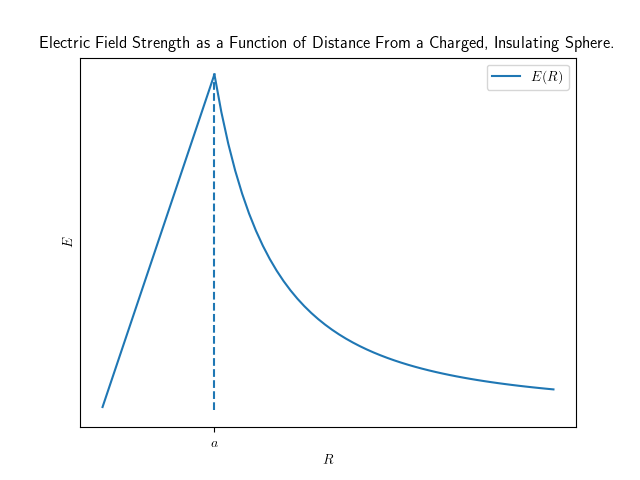
\includegraphics[scale=0.4]{electric_field_insulating_sphere.png}
            \caption{The electric field strength as a function of distance from the centre of a charged insulating sphere.}
            \label{fig:electric field strength insulating sphere}
        \end{subfigure}
        \begin{subfigure}{0.4\textwidth}
            \centering
            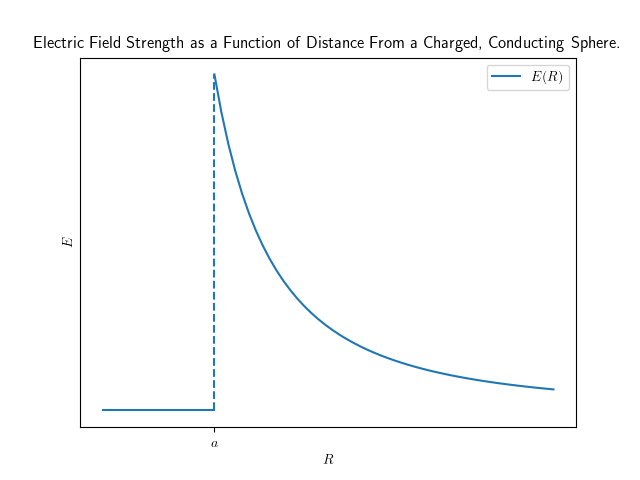
\includegraphics[scale=0.4]{electric_field_conducting_sphere.png}
            \caption{The electric field strength as a function of distance from the centre of a charged conducting sphere.}
            \label{fig:electric field strength conducting sphere}
        \end{subfigure}
        \caption{Electric field strength due to insulating and conducting spheres.}
    \end{figure}
    \subsubsection{Conducting Sphere}
    Consider now the same set up as above but the sphere is made of a conductor.
    Outside of the sphere all of the same logic applies and so for \(R > a\) we have
    \[E(R) = \frac{Q}{4\pi\varepsilon_0}\frac{1}{R^2} = \frac{\rho a^3}{3\varepsilon_0 R^2}.\]
    Inside the sphere the electric field is zero so we have \(E(R) = 0\) for \(R < a\).
    This is plotted in figure~\ref{fig:electric field strength conducting sphere}.
    
    \subsection{Cylindrical Symmetry}
    Take an infinitely long, thin wire with uniform charge density, \(\lambda\).
    We argue that by the symmetry of the situation the electric field must be
    \[\vv{E}(\vv{r}) = E(\rho)\ve{\rho}\]
    where we are working in cylindrical coordinates, \((\rho, \varphi, z)\).
    The argument for this is similar to the spherical case.
    If we place the origin on the wire, this is the only sensible choice for the location of the origin, then we are free to place it anywhere along the wire and we can define \(\varphi = 0\) as any position around the wire.
    This means that the field cannot depend on \(z\) or \(\varphi\) as then the origin position we pick would effect the field strength which is non-physical.
    Similarly if there is a component in the \(\ve{\varphi}\) direction then it must be the same all the way around the cylinder which means that there is a closed loop in the electric field meaning that \(\curl\vv{E} \ne \vv{0}\) which cannot be the case in an electrostatics situation.
    Finally the field can't have a component in the \(\ve{z}\) direction as this would cause motion of charge along the wire which would result in the charge distribution not being uniform.
    Therefore we are left only with dependence on \(\rho\) and a component in the direction \(\ve{\rho}\).
    
    Now construct a Gaussian surface of a cylinder of radius \(\rho\) which shares an axis with the wire.
    The field is always normal to this surface over the curved part so
    \[\vv{E}\cdot\dd{\vv{S}} = E(\rho)\ve{\rho}\cdot\dd{S}\ve{\rho} = E(\rho)\dd{S}.\]
    Over the flat ends of the cylinder the field is parallel to the surface so for the top surface
    \[\vv{E}\cdot\dd{\vv{S}} = E(\rho)\ve{\rho}\cdot\dd{S}\ve{z} = 0,\]
    the case of the bottom surface is the same but \(\dd{S}\) is negative.
    From Gauss' law we then have
    \begin{align*}
        \frac{Q_\mathrm{enc}}{\varepsilon_0} &= \oint_A \vv{E}\cdot\dd{\vv{S}}\\
        &= E(\rho)\int_{\mathrm{CSA}}\dd{S}\\
        &= E(\rho)2\pi\rho L
    \end{align*}
    where \(\mathrm{CSA}\) is the curved surface area of the cylinder and \(L\) is the length of the cylinder.
    The charge enclosed is simply \(Q_\mathrm{enc} = \lambda L\) so rearranging the above equation gives us
    \[E(\rho) = \frac{\lambda L}{\varepsilon}\frac{1}{2\pi\rho L} = \frac{\lambda}{2\pi\rho\varepsilon_0}.\]
    This is plotted in figure~\ref{fig:electric field strength of a charged wire}.
    \begin{figure}[ht]
        \centering
        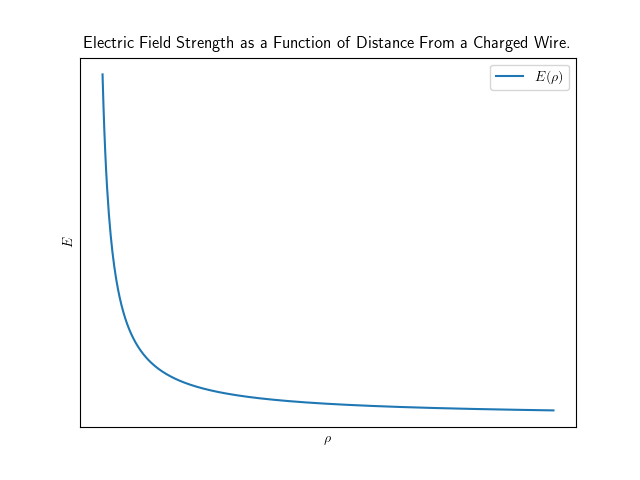
\includegraphics[scale=0.6]{electric_field_wire.png}
        \caption{The electric field strength due to a charged wire.}
        \label{fig:electric field strength of a charged wire}
    \end{figure}
    
    \subsection{Planar Symmetry}
    \subsubsection{Insulating Plane}
    Take an infinite plane with uniform charge density \(\sigma\).
    By symmetry we argue that
    \[\vv{E}(\vv{r}) = E(z)\ve{z}\]
    where we define \(\ve{z}\) as normal to the plane and place the origin in the plane.
    The argument for this is, again, similar to the previous arguments.
    Since we are free to place the origin anywhere in the plane there can be no \(x\) or \(y\) dependence in the field.
    We are also free to rotate the axis around the \(z\) axis which means that any component in the \(\ve{x}\) or \(\ve{y}\) direction must form a complete loop in the electric field which would mean \(\curl\ve{E} \ne \vv{0}\), this is not possible in electrostatics so there must be no \(\ve{x}\) or \(\ve{y}\) components.
    
    We choose a Gaussian surface that is a cylinder of radius \(R\).
    We place it so that its flat faces are parallel to the plane and one is above the plane and the other below.
    As well as this we have both faces the same distance from the plane.
    
    Along the curved surface the field is parallel to the surface so \(\vv{E}\cdot\dd{\vv{S}} = 0\).
    On the top face
    \[\vv{E}\cdot\dd{\vv{S}} = E(z)\ve{z}\cdot\dd{S}\ve{z} = E(z)\dd{S}.\]
    For the bottom case we have \(z < 0\).
    Since we are free to define \(z\)-axis in either direction we must have mirror symmetry in the \((x, y)\)-plane meaning that \(E(-z) = -E(z)\).
    This means that for the bottom face of the cylinder we have
    \[\vv{E}\cdot\dd{\vv{S}} = E(z)\ve{e}\cdot(-\dd{S}\ve{e}) = -E(z)\dd{S}.\]
    However since \(z < 0\) we have \(E(z) = E(-\abs{z}) = -E(\abs{z})\) so
    \[\vv{E}\cdot\dd{\vv{S}} = E(\abs{z})\dd{S}.\]
    This means that the contribution from the two faces is equal to twice the contribution from the top face.
    Applying Gauss' law we have
    \begin{align*}
        \frac{Q_\mathrm{enc}}{\varepsilon_0} &= \oint_A\vv{E}\cdot\dd{\vv{S}}\\
        &= E(z)\int_{2\circ}\dd{S}\\
        &= 2\pi R^2E(z)
    \end{align*}
    where \(2\circ\) is the two circular faces.
    The charge enclosed is \(Q_\mathrm{enc} = \pi R^2\sigma\) so rearranging the above equation gives us
    \[E(z) = \sgn(z)\frac{Q_\mathrm{enc}}{2\pi R^2\varepsilon_0} = \sgn(z)\frac{\pi R^2\sigma}{2\pi R^2\varepsilon_0} = \sgn(z)\frac{\sigma}{2\varepsilon_0},\]
    where
    \[
        \sgn(z) = 
        \begin{cases}
            1, & z > 0,\\
            0, & z = 0,\\
            -1, & z < 0.
        \end{cases}
    \]
    Notice that the only dependence on \(z\) is which side of the plane we are on as that affects the direction of the field.
    The field strength is constant.
    There is a discontinuous jump of \(\sigma/\varepsilon_0\) as we move from one side of the plane to the other.
    This is plotted in figure~\ref{fig:electric field insulated plane}
    \begin{figure}[ht]
        \centering
        \begin{subfigure}{0.4\textwidth}
            \centering
            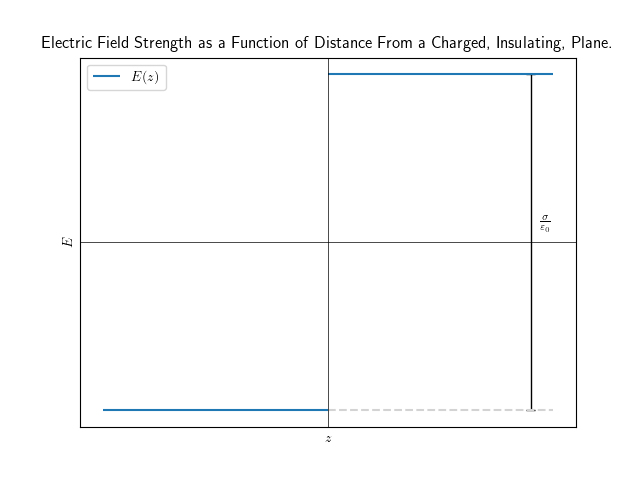
\includegraphics[scale=0.4]{electric_field_insulating_plane.png}
            \caption{Electric field strength as a function of distance from an insulating charged plane.}
            \label{fig:electric field insulated plane}
        \end{subfigure}
        \begin{subfigure}{0.4\textwidth}
            \centering
            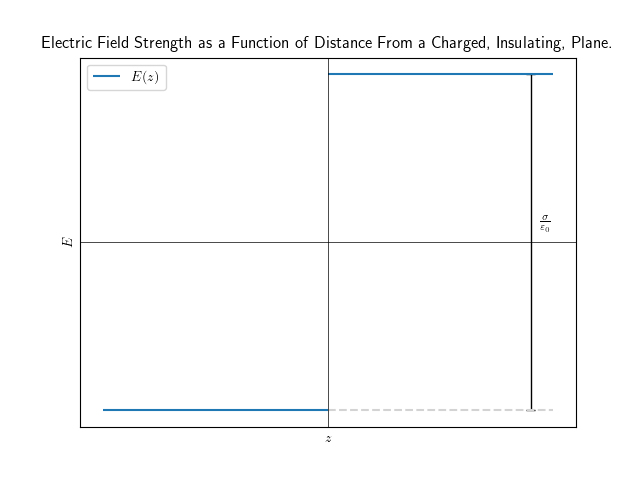
\includegraphics[scale=0.4]{electric_field_insulating_plane.png}
            \caption{Electric field strength as a function of distance from an insulating charged plane.}
            \label{fig:electric field conducting plane}
        \end{subfigure}
        \caption{Electric field strength due to insulating and conducting spheres.}
    \end{figure}
    If instead we have a conducting, charged, plane then the situation is a little different.
    By a conducting plane what we mean is that the plane is the surface of a conductor that continues on below the plane forever.
    The same logic as before works above the plane but now we have that the electric field below the plane is zero as it is inside a conductor.
    Thus
    \begin{align*}
        \frac{Q_\mathrm{enc}}{\varepsilon_0} &= \oint_A\vv{E}\cdot\dd{\vv{S}}\\
        &= E(z)\int_\circ \dd{S},\qquad z > 0\\
        &= E(z)\pi R^2\\
    \end{align*}
    So the electric field strength is
    \[
        E(z) = \begin{cases}
            \frac{\sigma}{\varepsilon_0}, & z > 0,\\
            0, & z \le 0.
        \end{cases}
    \]
    This is plotted in figure~\ref{fig:electric field conducting plane}.
    Note that in both cases there is a discontinuity of \(\sigma/\varepsilon_0\) when passing from one side of the plane to the other.
    
    \section{Poisson's Equation}
    \acrfull{pe} is a \acrfull{pde} of the form
    \[\laplacian\varphi = f\]
    where \(\varphi, f\colon\reals^3\to\reals\).
    The specific case of \(f(\vv{r}) = 0\) gives us
    \[\laplacian\varphi = 0\]
    which is \acrfull{le}.
    This crops up a lot in \acrshort{em} as the electrostatic potential and electric field are connected by
    \[\vv{E} = -\grad V\]
    and the electric field and charge density are related by Gauss' law:
    \[\div\vv{E} = \frac{\rho}{\varepsilon_0}.\]
    Combining these we get
    \[\div(\grad V) = \laplacian V = -\frac{\rho}{\varepsilon_0}.\]
    This simplifies to \acrshort{le} if \(\rho = 0\) everywhere in the region of interest.
    
    The most obvious solution to Laplace's equation is a potential of \(V(\vv{r}) = V_0\) for some constant \(V_0\).
    However as with all \acrshort{pde} there will be a set of \acrfull{bc} and typically \(V(\vv{r}) = V_0\) won't satisfy these \acrshort{bc}.
    Both \acrshort{pe} and \acrshort{le} are among the most important \acrshort{pde} in physics and appear in many scenarios.
    
    \subsection{Properties of Poisson's Equation}
    If \(V(\vv{r})\) is known then it is trivial to compute \(\rho(\vv{r}) = -\varepsilon\laplacian V\) or \(\vv{E}(\vv{r}) = -\grad V\).
    The more likely scenario however is that we know \(\rho(\vv{r})\) and we want to find the electric field.
    The first thing we should attempt should be to use Gauss' law, however this requires high levels of symmetry to be the most useful method.
    Lacking this symmetry the next thing that we can try to do is solve \acrshort{pe} for the potential.
    There is an explicit solution, given by the original definition of the potential:
    \[V(\vv{r}) = \frac{1}{4\pi\varepsilon_0}\int\frac{\rho(\vv{r'})}{\abs{\vv{r} - \vv{r'}}}\dd[3]{r'}.\]
    However this integral often has no analytic solution.
    There are methods for solving it numerically but this is not a numerical methods course so we won't discuss them.
    
    There are two useful properties of \acrshort{pe} that we use to find solutions:
    \begin{enumerate}
        \item The first useful property is linearity.
        If \(V_1\) and \(\rho_1\) satisfy \acrshort{pe} and \(V_2\) and \(\rho_2\) satisfy \acrshort{pe} then \(V_1 + V_2\) and \(\rho_1 + \rho_2\) satisfy \acrshort{pe}.
        That is
        \[\laplacian(V_1 + V_2) = -\frac{1}{\varepsilon_0}(\rho_1 + \rho_2).\]
        This follows trivially from the linearity of \(\laplacian\) as an operator which in turn follows from the linearity of partial derivatives as operators.
        In terms of \acrshort{em} this is just a restatement of the superposition principle.
        One use of this is if we have a shaped charge distribution, \(\rho\), that can be created from simpler shaped charged distributions, \(\rho_i\), then we can find the potential of each individual charge distribution and sum them together to get the potential of the entire charge distribution.
        For example a charged plane with a circular hole can be thought of as a plane without a hole and a charged disc the size of the hole, at the same position but with the opposite charge to the plane over he same area.
        
        \item The second useful property is that the solution to \acrshort{pe} is unique (possibly up to a constant term) for a given set of \acrshort{bc}.
        There are two common ways that \acrshort{bc} are given:
        \begin{itemize}
            \item \(V\) is specified on the boundary -- known as Dirichlet \acrshort{bc}.
            The solution will be unique.
            \item \(\vv{E}\) is specified on the boundary -- known as Neumann \acrshort{bc}.
            The solution will be unique up to a constant term.
        \end{itemize}
    \end{enumerate}
    
    \subsubsection{Proof of Uniqueness}
    \begin{theorem}
        Consider a region, \(\region\), with boundary, \(\boundary\)\footnote{It is possible that the boundary could be at infinity.}.
        Let \(\rho(\vv{r})\) be specified within \(\region\).
        Let the \acrshort{bc} be given by either
        \begin{enumerate}
            \item \(V\) is specified on \(\boundary\).
            \item \(\vv{E} = -\grad V\) is specified on \(\boundary\).
        \end{enumerate}
        Then any solution of \acrfull{pe},
        \[\laplacian V = -\frac{\rho}{\varepsilon_0},\]
        which satisfies the boundary conditions is unique (up to a constant term in the case of the second set of boundary conditions.)
    \end{theorem}
    \begin{proof}
        Suppose that \(V_1\) and \(V_2\) are two distinct solutions to \(\laplacian V = -\rho/\varepsilon_0\).
        Define \(\psi = V_1 - V_2\).
        Then
        \begin{align*}
            \laplacian \psi &= \laplacian(V_1 - V_2)\\
            &= \laplacian V_1 - \laplacian V_2\\
            &= \rho - \rho\\
            &= 0.
        \end{align*}
        Thus \(\psi\) is a solution to \acrshort{le}.
        Multiplying by \(\psi\) we have
        \[\psi\laplacian\psi = \psi\cdot0 = 0.\]
        Consider the following:
        \[\div(\psi\grad\psi) - (\grad\psi)\cdot(\grad\psi)\]
        Applying the product rule for the divergence of the product of a scalar field and vector field to the first term we get
        \[(\div\psi)\cdot(\div\psi) - \psi(\div(\grad\psi) - (\grad\psi)\cdot(\grad\psi).\]
        The first and last terms cancel and we are left with
        \[\psi(\div(\grad\psi)) = \psi\laplacian\psi = 0.\]
        So the whole term is zero over the whole of \(\region\).
        This means that integrating this term over \(\region\) will also be zero:
        \[\int_\region \div(\psi\grad\psi) - (\grad\psi)\cdot(\grad\psi)\dd{V} = 0.\]
        Applying the divergence theorem to the first term this becomes
        \[\int_\boundary \psi\grad\psi\cdot\dd{\vv{S}} - \int_\region (\grad\psi)\cdot(\grad\psi) \dd{V} = 0.\]
        For either set of boundary conditions the first term is zero.
        The second term is nonnegative everywhere as the integrand is the norm of a vector.
        Therefore for the integral to be zero we must have that the integrand is zero.
        The norm of a vector is only zero when that vector is zero therefore
        \[\grad\psi = 0.\]
        This means that \(\psi = V_1 - V_2\) is constant.
        So \(V_1\) and \(V_2\) differ by at most a constant.
        If the boundary conditions were given in terms of \(V\) at \(\boundary\) then we know that \(V_1 = V_2\) at the boundaries so this constant is zero.
    \end{proof}
    
    \begin{example}
        Consider a cavity, \(\region\), in a conductor.
        We claim that if \(\rho = 0\) in the cavity then \(\vv{E} = \vv{0}\) inside the cavity.
        
        The inner surface of the conductor is an equipotential since it is conducting.
        This means that \(V = V_0\) for some constant \(V_0\).
        This is our \acrshort{bc}.
        Inside the cavity we have \(\laplacian V = 0\) since there is no charge.
        Thus we have to solve \acrshort{le} subject to the condition that \(V = V_0\) on the boundary.
        One solution to this is \(V = V_0\) everywhere in \(\region\).
        By the uniqueness theorem above we know that this is the only solution.
        Now we simply compute \(\vv{E} = -\grad V = -\grad V_0 = \vv{0}\).
    \end{example}
    
    \subsection{The Method of Images}
    The method of images is a method for solving \acrshort{pe} by placing `image charges' outside of the region, \(\region\), such that they reproduce the required \acrshort{bc}.
    These charges don't affect \acrshort{pe} inside \(\region\) as they aren't in the region so don't change \(\rho\) in the region.
    However the field that results from the superposition of these image charges as well as any pre-existing charges is the correct solution to \acrshort{pe}.
    
    \begin{example}
        Consider a conducting plane with a point charge, \(Q\), placed a distance \(a\) above the plane.
        What is the potential in the region, \(\region\), above the plane?
        
        The charge density above the plane is
        \[\rho(\vv{r}) = Q\delta(z - a)\delta(x)\delta(y)\]
        where we have placed the origin in the plane directly below the charge and have the \(z\)-axis normal to the plane.
        Our boundary condition is that \(V(x, y, 0) = 0\) as at the plane \(\vv{E} = 0\) so \(V = V_0\) and we choose \(V_0 = 0\) for simplicity.
        
        Unfortunately \(V = V_0\) is not a solution to \acrshort{pe} here as we know that the potential from a point charge falls away as \(1/r\) so at the origin (in the plane directly below the charge) we expect the potential to be \(V = 1/a\) of what it is at the point charge.
        We need to solve
        \[\laplacian V(\vv{r}) = -\frac{\rho(\vv{r})}{\varepsilon_0}.\]
        To do this we can add a homogenous solution, \(V_\text{im}\) to \acrshort{pe}.
        By homogenous here we mean that \(\laplacian V_\text{im} = 0\), i.e. a solution to \acrshort{le}.
        This solution only needs to be homogeneous for \(z \ge 0\) since this is the region of interest.
        We know that the potential due to the point charge is
        \[V_Q(\vv{r}) = \frac{Q}{r\pi\varepsilon_0}\frac{1}{\sqrt{x^2 + y^2 + (z - a)^2}}.\]
        We place an image charge, \(-Q\), at \(z = -a\) which gives us an image potential of
        \[V_\text{im}(\vv{r}) = -\frac{Q}{r\i\varepsilon_0}\frac{1}{\sqrt{x^2 + y^2 + (z + a)^2}}.\]
        At every point on the plane we have
        \[V_Q + V_\text{im} = \frac{Q}{r\i\varepsilon_0}\frac{1}{\sqrt{x^2 + y^2 + (0 - a)^2}} - \frac{Q}{r\i\varepsilon_0}\frac{1}{\sqrt{x^2 + y^2 + (0 + a)^2}} = 0\]
        so the boundary conditions are satisfied.
        Thus \(V = V_Q + V_\text{im}\) is the solution and gives the potential everywhere.
        
        In reality this potential isn't caused by two point charges.
        Rather the real point charge causes the charge density of the plane to become non-uniform in a way that the final potential is as given above.
    \end{example}
    
    \section{Electric Dipoles and Multipoles}
    The motivation behind this section is to study a general, non-trivial, charge distribution, \(\rho(\vv{r})\), and in particular find an approximation of the potential,
    \[V(\vv{r}) = \frac{1}{4\pi\varepsilon_0}\int\frac{\rho(\vv{r'})}{\abs{\vv{r} - \vv{r'}}}\dd[3]{r'},\]
    which applies to points, \(\vv{r}\), far from where \(\rho(\vv{\vv{r'}}) \ne 0\).
    
    \subsection{Electric Dipoles}
    An \define{electric dipole} is formed from two charges, \(\pm q\), fixed distance \(a\) apart.
    The vector from \(q\) to \(-q\) is defined to be \(\vv{a}\).
    The \define{electric dipole moment} is then defined to be \(\vv{p} = q\vv{a}\).
    An electric dipole is shown in figure~\ref{fig:electric dipole}.
    \begin{figure}[ht]
        \centering
        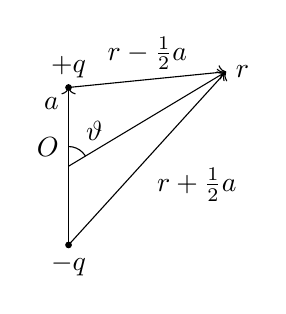
\begin{tikzpicture}
            \draw[fill=black] (0, 1) circle[radius=0.035cm];
            \draw[fill=black] (0, -1) circle[radius=0.035cm];
            \node[above] at (0, 1) {\(+q\)};
            \node[below] at (0, -1) {\(-q\)};
            \node[above left] at (0, 0) {\(O\)};
            \draw[->] (0, -1) -- (0, 1);
            \node[below left] at (0, 1) {\(\vv{a}\)};
            \draw[->] (0, 1) -- (2, 1.2);
            \draw[->] (0, -1) -- (2, 1.2);
            \draw[->] (0, 0) -- (2, 1.2);
            \node[right] at (2, 1.2) {\(\vv{r}\)};
            \begin{scope}
                \clip (0, 0) -- (0, 1) -- (2, 1.2) -- cycle;
                \draw (0, 0) circle[radius=0.25cm];
            \end{scope}
            \node[above right] at (0.1, 0.2) {\(\vartheta\)};
            \node[above] at (1, 1.1) {\(\vv{r} - \frac{1}{2}\vv{a}\)};
            \node[below right] at (1, 0.1) {\(\vv{r} + \frac{1}{2}\vv{a}\)};
        \end{tikzpicture}
        \caption{An electric dipole.}
        \label{fig:electric dipole}
    \end{figure}
    Dipoles like this are important because many molecules, such as \ce{H2O} and \ce{CO} have permanent dipoles and all molecules/atoms acquire an induced dipole in an external field.
    
    \subsubsection{Field of an Electric Dipole}
    The electric potential of an electric dipole is simply the superposition of the potential due to the two point charges:
    \[V(\vv{r}) = \frac{q}{4\pi\varepsilon_0}\left(\frac{1}{r_+} - \frac{1}{r_-}\right)\]
    where 
    \[\vv{r_{\pm}} = \vv{r} \mp \frac{1}{2}\vv{a}.\]
    That is \(\vv{r_\pm}\) is the vector from \(\pm q\) to \(\vv{r}\).
    The next question that we ask is what is the field like for \(r \gg a\)?
    This is known as the far field approximation.
    We can Taylor expand the \(1/r_\pm\) terms in the potential.
    To do this we first note that
    \begin{align*}
        r_\pm^2 &= \vv{r_\pm}\cdot\vv{r_\pm}\\
        &= \left(\vv{r} \mp \frac{1}{2}\vv{a}\right)\cdot\left(\vv{r} \mp \frac{1}{2}\vv{a}\right)\\
        &= r^2 \mp \vv{a}\cdot\vv{r} + \frac{1}{4}a^2\\
        &= r^2 \mp  ar\cos\vartheta + \frac{1}{4}a^2\\
        &= r^2\left(1 \mp \frac{a}{r}\cos\vartheta + \frac{a^2}{4r^2}\right).
    \end{align*}
    Hence
    \[\frac{1}{r_\pm} = \left[r^2\left(1 \mp \frac{a}{r}\cos\vartheta + \frac{a^2}{4r^2}\right)\right]^{-1/2} = \frac{1}{r}\left[\left(1 \mp \frac{a}{r}\cos\vartheta + \frac{a^2}{4r^2}\right)\right]^{-1/2}.\]
    For \(r > a\) this is of the form \((1 + \varepsilon)^p\) with \(\abs{\varepsilon} < 1\) needed to use
    \[(1 + \varepsilon)^p = 1 + p\varepsilon + \order{\varepsilon^2}.\]
    Doing this gives
    \begin{align*}
        \frac{1}{r_\pm} &= \frac{1}{r}\left[1 - \frac{1}{2}\left(\mp\frac{a}{r}\cos\vartheta + \frac{a^2}{4r^2}\right) + \order{\frac{a^2}{r^2}}\right]\\
        &= \frac{1}{r} \pm \frac{a}{2r^2}\cos\vartheta + \order{\frac{a^2}{r^3}}.
    \end{align*}
    Substituting this into the potential gives
    \begin{align*}
        V(\vv{r}) &= \frac{q}{4\pi\varepsilon_0}\left(\frac{1}{r_+} - \frac{1}{r_-}\right)\\
        &\approx \frac{q}{4\pi\varepsilon_0}\left(\frac{1}{r} + \frac{a}{2r^2}\cos\vartheta - \frac{1}{r} + \frac{a}{2r^2}\cos\vartheta\right)\\
        &= \frac{qa\cos\vartheta}{r^2\pi\varepsilon_0}\\
        &= \frac{\vv{p}\cdot\vh{r}}{4\pi\varepsilon_0r^2}.
    \end{align*}
    Notice that this drops off as \(1/r^2\) whereas the potential from a point charge drops off slower as \(1/r\).
    You can think of this as the fact that there are positive and negative charges close together causing parts of the potential to cancel.
    What we have derived here is the far field limit, in that it is only valid for \(r \gg a\).
    It is also known as the `ideal dipole' potential which is what we would get if we too a limit as \(a \to 0\), and \(q\to\infty\) in such a way that \(\vv{p}\) remains constant.
    
    \subsubsection{Dipole Interaction With an External Electric Field}
    The electrostatic energy of a point charge, \(q\), in a potential, \(V\), is \(U = qV\).
    The energy of a dipole is then the superposition of the two point charges:
    \[U_\text{dip} = qV_\text{ext}(\vv{a}/2) - qV_\text{ext}(-\vv{a}/2).\]
    Here \(V_\text{ext}\) is the external potential.
    Taking a Taylor series gives
    \begin{align*}
        U_\text{dip} &\approx q\left[V_\text{ext}(0) + \frac{1}{2}\vv{a}\cdot\grad V_\text{ext}\right] - q\left[V_\text{ext}(0) - \frac{1}{2}\vv{a}\cdot\grad V_\text{ext}\right]\\
        &= q\vv{a}\cdot\grad V_\text{ext}\\
        &= -q\vv{a}\cdot\vv{E_\mathrm{ext}}\\
        &= -p\cdot\vv{E_\mathrm{ext}}
    \end{align*}
    We see that the dipole energy is minimised if \(\vv{p}\) is parallel to \(\vv{E_\mathrm{ext}}\) and the energy is maximised when they are antiparallel.
    The change in energy to change between parallel and antiparallel is
    \[\Delta U = 2p\abs{E_\mathrm{ext}}.\]
    The force experienced by the dipole is
    \[\vv{F} = -\grad U_\text{dip} = \grad(\vv{p\cdot\vv{E_\mathrm{ext}}}).\]
    If \(\vv{E_\mathrm{ext}}\) is a uniform field (doesn't depend on \(\vv{r}\)) then the force is zero.
    This is because the two charges experience equal and opposite forces.
    However there is still a torque because the two charges aren't in the same location.
    This torque acts to align the dipole with \(\vv{E_\mathrm{ext}}\) and is given by:
    \[\vv{\tau} = \frac{1}{2}\vv{a}\times q\vv{E_\mathrm{ext}} - \frac{1}{2}\vv{a}\times(-q\vv{E_\mathrm{ext}}) = \vv{p}\times\vv{E_\mathrm{ext}}.\]
    The work done by the torque to rotate the dipole from aligned with the field to an angle \(\vartheta\) from the field is
    \[W = \int_0^\vartheta \tau\dd{\vartheta} = \int_0^\vartheta qE_\mathrm{ext}\dd{\vartheta} = pE_\mathrm{ext}(1 - \cos\vartheta).\]
    In a non-uniform field the force is generally more complex.
    It acts to move the dipole along the gradient of the field.
    
    \subsection{Multipole Expansion}
    Given a charge distribution \(\rho\) we say that \(\rho\) is bounded inside a region, \(\region\), if, for \(\vv{r}\notin\region\), \(\rho(\vv{r}) = 0\).
    Let \(\rho\) be a charge distribution that is bounded inside the region \(\region\).
    Then from the definition of the potential we know that
    \[V(\vv{r}) = \frac{1}{4\pi\varepsilon_0} \int_\region \frac{\rho(\vv{r'})}{\abs{\vv{r} - \vv{r'}}}\dd[3]{r'}.\]
    This holds for all \(\vv{r}\).
    However if \(\vv{r}\notin\region\), that is \(r \gg r'\), then we can make use of a Taylor expansion.
    Following the same steps as we did for a dipole we see that
    \[\frac{1}{\abs{\vv{r} - \vv{r'}}} = \frac{1}{r}\left[1 - \frac{2\vv{r}\cdot\vv{r'}}{r^2} + \frac{r'^2}{r^2}\right]^{-1/2}.\]
    We now Taylor expand this but keep higher order terms:
    \begin{align*}
        \left[1 - \frac{2\vv{r}\cdot\vv{r'}}{r^2} + \frac{r'^2}{r^2}\right]^{-1/2} &= 1 - \frac{1}{2}\left(-\frac{2\vv{r}\cdot\vv{r'}}{r^2} + \frac{r'^2}{r^2}\right) + \frac{3}{8}\left(-\frac{2\vv{r}\cdot\vv{r'}}{r^2} + \frac{r'^2}{r^2}\right)^2 + \order{\frac{1}{r^3}}\\
        &= 1 + \frac{\vv{r}\cdot\vv{r'}}{r^2} - \frac{1}{2}\frac{r'^2}{r^2} + \frac{3}{2}\frac{(\vv{r}\cdot\vv{r'})^2}{r^4} - \frac{3}{2}\frac{r'^2(\vv{r}\cdot\vv{r'})}{r^4} - \frac{3}{8}\frac{r'^4}{r^4} + \order{\frac{1}{r^3}}\\
        &= 1 + \frac{\vh{r}\cdot\vv{r'}}{r} - \frac{1}{2}\frac{r'^2}{r^2} + \frac{3}{2}\frac{(\vh{r}\cdot\vv{r'})^2}{r^2} - \frac{3}{2}\frac{r'^2(\vh{r}\cdot\vv{r})}{r^3} - \frac{3}{8}\frac{r'^4}{r^4} + \order{\frac{1}{r^3}}
        \shortintertext{keeping only terms of order \(1/r^2\) or lower}
        &\approx 1 + \frac{\vh{r}\cdot\vv{r'}}{r} - \frac{1}{2}\frac{r'^2}{r^2} + \frac{3}{4}\frac{(\vh{r}\cdot\vv{r'})^2}{r^2}\\
        &= 1 + \frac{\vh{r}\cdot\vv{r'}}{r} + \frac{3(\vh{r}\cdot\vv{r'}) - r'^2}{2r^2}
    \end{align*}
    Using this in the definition of the potential gives
    \begin{align*}
        V(\vv{r}) &\approx \frac{1}{4\pi\varepsilon_0}\int_\region \dd[3]{r'} \rho(\vv{r'})\frac{1}{r}\left[1 + \frac{\vh{r}\cdot\vv{r'}}{r} + \frac{3(\vh{r}\cdot\vv{r'}) - r'^2}{2r^2}\right]\\
        &= \frac{1}{4\pi\varepsilon_0}\int_\region \dd[3]{r'} \rho(\vv{r'})\left[\frac{1}{r} + \frac{\vh{r}\cdot\vv{r'}}{r^2} + \frac{3(\vh{r}\cdot\vv{r'}) - r'^2}{2r^3}\right].
    \end{align*}
    Defining some new terms this becomes
    \[V(\vv{r}) \approx \frac{1}{4\pi\varepsilon_0}\frac{Q}{r} + \frac{1}{r\pi\varepsilon_0}\frac{\vh{r}\cdot\vv{P}}{r^2} + \frac{1}{4\pi\varepsilon_0}\frac{1}{r^3}\frac{1}{2}\sum_{i, j}\quadrupole_{ij}\hat{r}_i\hat{r}_j.\]
    Where
    \[Q = \int_\region \dd[3]{r'}\rho(\vv{r'})\]
    is the total charge,
    \[\vv{P} = \int_\region \dd[3]{r'}\vv{r'}\rho(\vv{r'})\]
    is the net dipole moment, a vector with Cartesian components
    \[P_i = \int_\region \dd[3]{r'}r'_i\rho(\vv{r'}),\]
    and \(\quadrupole\) is the quadrupole tensor which has Cartesian components
    \[\quadrupole_{ij} = \int_\region\dd[3]{r'}(3r'_ir'_j - r'^2\delta_{ij})\rho(\vv{r'}).\]
    This representation of \(V\) is the \define{multipole expansion} of \(V\) in Cartesian coordinates.
    The first term is the monopole term.
    It is dominant when \(Q\ne 0\) and reasonably approximates the far field charge distribution as a point charge at the origin.
    When the total charge, \(Q\), is zero then the second term, the dipole term, dominates.
    If this term also vanishes then the third term, the quadrupole term, dominates.
    Note that another way of writing this terms is
    \[\frac{1}{4\pi\varepsilon_0}\frac{1}{r^3}\frac{1}{2} \vh{r}\trans\quadrupole\vh{r} = \frac{1}{4\pi\varepsilon_0}\frac{1}{r^5}\frac{1}{2} \vv{r}\trans\quadrupole\vv{r}.\]
    It is possible to take even more terms of the Taylor series and end up with more terms, however we will stop at three.
    Note that each term of the expansion is a solution to \gls{le} and therefore we can use the method of images with image dipoles and quadrupoles as well as image charges.
    
    \begin{example}\label{exa:dipole moment}
        \begin{figure}[ht]
            \centering
            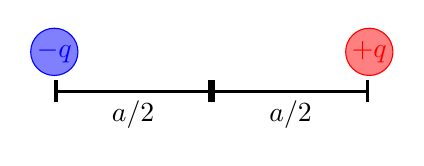
\begin{tikzpicture}
                \draw[color=red, fill=red!50!white] (2, 0) circle[radius=0.3cm];
                \draw[color=blue, fill=blue!50!white] (-2, 0) circle[radius=0.3cm];
                \draw[very thick, |-|] (-2, -0.5) -- (0, -0.5);
                \draw[very thick, |-|] (0, -0.5) -- (2, -0.5);
                \node[red] at (2, 0) {\(+q\)};
                \node[blue] at (-2, 0) {\(-q\)};
                \node[below] at (-1, -0.5) {\(a/2\)};
                \node[below] at (1, -0.5) {\(a/2\)};
            \end{tikzpicture}
            \caption{The dipole setup used in example~\ref{exa:dipole moment}}
        \end{figure}
        A dipole formed of two charges, \(\pm q\), aligned along the \(x\)-axis so that \(q\) is at \((a/2, 0, 0)\) and \(-q\) is at \((-a/2, 0, 0)\) has a charge density given by
        \[\rho(\vv{r}) = q[\delta(x - a/2) - \delta(x + a/2)]\delta(y)\delta(z).\]
        Clearly \(Q = 0\).
        The \(x\) component of the dipole moment is
        \begin{align*}
            P_x &= \int x\rho(\vv{r})\dd{V}\\
            &= q\int x[\delta(x - a/2) - \delta(x + a/2)]\dd{x}\int\delta(y)\dd{y}\int\delta(z)\dd{z}\\
            &= q\frac{a}{2} - q\left(\frac{a}{2}\right)\\
            &= qa.
        \end{align*}
        The \(y\) component is
        \begin{align*}
            P_y &= \int y\rho(\vv{r})\dd{V}\\
            &= \int[\delta(x - a/2) - \delta(x + a/2)]\dd{x}\int y\delta(y)\dd{y}\int \delta(z)\dd{z}\\
            &= 0
        \end{align*}
        since the middle integral is zero.
        Similarly we can show that \(P_z = 0\).
        This means that \(\vv{P} = q\vv{a}\), so we are justified in calling \(\vv{P}\) the dipole moment.
    \end{example}
    \begin{example}\label{exa:quadrupole moment}
        \begin{figure}[ht]
            \centering
            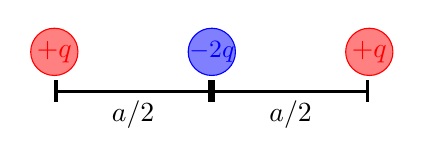
\begin{tikzpicture}
                \draw[color=red, fill=red!50!white] (-2, 0) circle[radius=0.3cm];
                \draw[color=red, fill=red!50!white] (2, 0) circle[radius=0.3cm];
                \draw[color=blue, fill=blue!50!white] (0, 0) circle[radius=0.3cm];
                \node[color=red] at (-2, 0) {\(+q\)};
                \node[color=red] at (2, 0) {\(+q\)};
                \node[color=blue] at (0, 0) {\small\(-2q\)};
                \draw[very thick, |-|] (-2, -0.5) -- (0, -0.5);
                \draw[very thick, |-|] (0, -0.5) -- (2, -0.5);
                \node[below] at (-1, -0.5) {\(a/2\)};
                \node[below] at (1, -0.5) {\(a/2\)};
            \end{tikzpicture}
            \caption{The quadrupole setup used in example~\ref{exa:quadrupole moment}}
        \end{figure}
        Three charges are placed in a line along the \(x\)-axis.
        Two of the charges have charge \(q\) and are at \(\pm a/2\).
        The third charge is at the origin and has charge \(-2q\).
        The charge density is
        \[\rho(\vv{r}) = q[\delta(x - a/2) + \delta(x + a/2) - 2\delta(x)]\delta(y)\delta(z).\]
        Again, \(Q = 0\).
        The \(x\) component of the dipole moment is
        \begin{align*}
            P_x &= \int x\rho(\vv{r})\dd{V}\\
            &= q\int x[\delta(x - a/2) + \delta(x + a/2) - 2\delta(x)]\int\delta(y)\dd{y}\int\delta(z)\dd{z}\\
            &= q\left[\frac{a}{2} - \frac{a}{2} + 0\right]\\
            &= 0
        \end{align*}
        In a similar way to the previous example \(P_y = P_z = 0\).
        Thus the dipole moment vanishes.
        
        Next we calculate the quadrupole moment.
        In general
        \[\quadrupole_{ij} = \int(3x_ix_j - r^2\delta_{ij})\rho(\vv{r})\dd{V}.\]
        The \(\quadrupole_{xx}\) component is
        \begin{align*}
            \quadrupole_{xx} &= \int(3x^2 - r^2)q[\delta(x - a/2) + \delta(x + a/2) - 2\delta(x)]\delta(y) \delta(z)\dd{V}\\
            &= \int(3x^2 - (x^2 + y^2 + z^2))q[\delta(x - a/2) + \delta(x + a/2) - 2\delta(x)]\delta(y) \delta(z)\dd{V}\\
            &= 3q\left(\frac{a}{2}\right)^2 - q\left(\frac{a}{2}\right)^2 + 3q\left(-\frac{a}{2}\right)^2 - q\left(-\frac{a}{2}\right)^2\\
            &= qa^2
        \end{align*}
        Next we will calculate \(\quadrupole_{xy}\):
        \begin{align*}
            \quadrupole_{xy} &= \int 3xyq[\delta(x - a/2) + \delta(x + a/2) - 2\delta(x)]\delta(y) \delta(z)\dd{V}\\
            &= \int 3xq[\delta(x - a/2) + \delta(x + a/2) - 2\delta(x)]\dd{x}\int y\delta(y)\dd{y} \int\delta(z)\dd{z}\\
            &= 0
        \end{align*}
        If we calculated every component we would find that
        \[
            \quadrupole = qa^2
            \begin{pmatrix}
                1 & 0 & 0\\
                0 & -\frac{1}{2} & 0\\
                0 & 0 & -\frac{1}{2}
            \end{pmatrix}
            .
        \]
        We can then approximate the potential as
        \begin{align*}
            V(\vv{r}) &= \frac{1}{8\pi\varepsilon_0} \frac{1}{r^5}\vv{r}\trans\quadrupole\vv{r}\\
            &= \frac{qa^2}{8\pi\varepsilon_0}\frac{1}{r^5}
            \begin{pmatrix}
                x & y & z
            \end{pmatrix}
            \begin{pmatrix}
                1 & 0 & 0\\
                0 & -\frac{1}{2} & 0\\
                0 & 0 & -\frac{1}{2}
            \end{pmatrix}
            \begin{pmatrix}
                x\\ y\\ z
            \end{pmatrix}
            \\
            &= \frac{qa^2}{8\pi\varepsilon_0}\frac{1}{r^5}
            \begin{pmatrix}
                x & y & z
            \end{pmatrix}
            \begin{pmatrix}
                x\\ -\frac{1}{2}y\\ -\frac{1}{2}z
            \end{pmatrix}
            \\
            &= \frac{qa^2}{8\pi\varepsilon_0}\frac{1}{r^5}
            \left[x^2 - \frac{1}{2}(y^2 + z^2)\right].
        \end{align*}
    \end{example}
    \begin{example}\label{exa:quadrupole moment 2}
        \begin{figure}[ht]
            \centering
            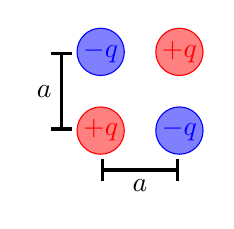
\begin{tikzpicture}
                \draw[color=red, fill=red!50!white] (0, 0) circle[radius=0.3cm];
                \draw[color=blue, fill=blue!50!white] (1, 0) circle[radius=0.3cm];
                \draw[color=blue, fill=blue!50!white] (0, 1) circle[radius=0.3cm];
                \draw[color=red, fill=red!50!white] (1, 1) circle[radius=0.3cm];
                \node[color=red] at (0, 0) {\(+q\)};
                \node[color=blue] at (1, 0) {\(-q\)};
                \node[color=blue] at (0, 1) {\(-q\)};
                \node[color=red] at (1, 1) {\(+q\)};
                \draw[very thick, |-|] (0, -0.5) -- (1, -0.5);
                \draw[very thick, |-|] (-0.5, 0) -- (-0.5, 1);
                \node[below] at (0.5, -0.5) {\(a\)};
                \node[left] at (-0.5, 0.5) {\(a\)};
            \end{tikzpicture}
            \caption{The quadrupole setup used in example~\ref{exa:quadrupole moment 2}}
        \end{figure}
        Four charges \(\pm q\) are placed on the corners of a square in the \((x, y)\)-plane with side length \(a\) with the origin at the centre of the square.
        They are arranged such that diagonally opposite charges have the same sign and charges connected by an edge have opposite signs.
        The charge density is
        
        \begin{multline*}
            \rho(\vv{r}) = q[\delta(x - a/2)\delta(y - a/2) - \delta(x + a/2)\delta(y - a/2) \\- \delta(x - a/2)\delta(y + a/2) + \delta(x + a/2)\delta(y + a/2)]\delta(z).
        \end{multline*}
        Again it can be shown that \(\vv{P} = \vv{0}\) and clearly \(Q = 0\).
        If we calculate the quadrupole components then we find that
        \[
            \quadrupole = qa^2
            \begin{pmatrix}
                0 & 3 & 0\\
                3 & 0 & 0\\
                0 & 0 & -2
            \end{pmatrix}
            .
        \]
        The potential can then be approximated as
        \[V(\vv{r}) = \frac{qa^2}{8\pi\varepsilon_0}\frac{1}{r^5}[6xy - 2z^2].\]
    \end{example}

    \section{Electrostatic Energy and Capacitors}
    \subsection{Electrostatic Energy of a General Charge Distribution}\label{sec:energy electric field}
    If we start with an assembly of \(n - 1\) point charges, \(q_i\), at position \(\vv{r_i}\) then the potential at \(\vv{r}\) is given by the superposition of the potentials of each particle:
    \[V(\vv{r}) = \frac{1}{4\pi\varepsilon_0}\sum_{j=1}^{n-1}\frac{q_i}{\abs{\vv{r} - \vv{r_j}}}.\]
    If we then bring another charge, \(q_n\), from infinity to \(\vv{r_n}\) then the work required to do so is
    \[W_n = q_nV(\vv{r_n}) = \frac{q_n}{\frac{q_n}{4\pi\varepsilon_0}} \sum_{j=1}^{n-1}\frac{q_j}{\abs{\vv{r_n} - \vv{r_j}}}.\]
    We can write out this sum for the first few values of \(n\) to see how it progresses:
    \begin{align*}
        W_1 &= 0\\
        W_2 &= \frac{q_2q_1}{4\pi\varepsilon_0}\frac{1}{\abs{\vv{r_2} - \vv{r_1}}}\\
        W_3 &= \frac{q_3q_1}{4\pi\varepsilon_0}\frac{1}{\abs{\vv{r_3} - \vv{r_1}}} + \frac{q_3q_2}{4\pi\varepsilon_0}\frac{1}{\abs{\vv{r_3} - \vv{r_2}}}
    \end{align*}
    In general the total work required to assemble \(n\) charges, which is the electrostatic energy, \(U_E\), is given by
    \begin{align*}
        U_E &= \sum_{i=1}^{n}W_i\\
        &= \frac{1}{4\pi\varepsilon_0}\sum_{i=1}^{n}\sum_{j=1}^{i - 1}\frac{q_iq_j}{\abs{\vv{r_i} - \vv{r_j}}}\\
        &= \frac{1}{8\pi\varepsilon_0}\sum_{\stackrel{i, j}{i\ne j}}^{n}\frac{q_iq_j}{\abs{\vv{r_i} - \vv{r_j}}}.
    \end{align*}
    In the last step we collapsed two sums into one by noting that a sum over \(i\) and \(j\) with \(i > j\) is equivalent to a sum over \(i\) and \(j\) with \(i \ne j\) except that the second allows for \((i,j) = (2,1)\) and \((i,j)=(1,2)\).
    Due to symmetry the value of both of these terms is the same so we end up double counting the allowed states where \(i > j\) if we include all \(j \ne i\).
    For this reason we have to divide by 2 which explains the factor of \(8\) in the denominator.
    
    In the limit of a continuous charge density, \(\rho\), the electrostatic energy is
    \[U_E = \frac{1}{2}\int\rho(\vv{r})V(\vv{r})\dd[3]{r}.\]
    Using Maxwell's first law this becomes
    \[U_E = \frac{\varepsilon_0}{2}\int V(\vv{r})(\div\vv{E})\dd[3]{r}.\]
    We then use the product rule,
    \[\div(V\vv{E}) = V\div\vv{E} + (\grad V)\cdot\vv{E} = V\div\vv{E} - \vv{E}\cdot\vv{E} = V\div\vv{E} - E^2,\]
    to change the integrand to
    \[U_E = \frac{\varepsilon_0}{2}\int \div[V(\vv{r})\vv{E}(\vv{r})] + E^2\dd[3]{r}.\]
    Splitting the integral at the addition and applying the divergence theorem to the first integral we get
    \[U_E = \frac{\varepsilon_0}{2}\oint_SV(\vv{r})\vv{E}(\vv{r})\cdot\dd{\vv{S}} + \frac{\varepsilon_0}{2}\int E^2\dd[3]{r}.\]
    So far we have made no assumptions about the volume over which our integration occurs.
    This means we are free to pick any boundary, \(S\).
    We choose \(S\) to be at infinity.
    Assuming that our charge distribution is bound we know that outside of the region containing it \(V\) drops of as at least \(1/r\) and \(E\) drops off as at least \(1/r^2\).
    Thus \(VE\) drops of as at least \(1/r^3\).
    The area of the surface however only grows as \(1/r^2\) so the first integral must be zero.
    Thus the internal energy is
    \[U_E = \frac{\varepsilon_0}{2}\int \abs{\vv{E}(\vv{r})}^2\dd[3]{r} = \int u_E \dd[3]{r},\]
    where
    \[u_E = \frac{\varepsilon_0}{2}\abs{\vv{E}(\vv{r})}^2\]
    is the energy density.
    
    Note that this derivation started from a continuous charge distribution.
    This does not apply to point charges.
    If we were to apply it to point charges there are self interaction terms that we would have to exclude.
    We can see this form the point charge equations, if we try to include the interaction of a point charge with itself we get \(\abs{\vv{r_i} - \vv{r_i}} = 0\) so we end up dividing by zero.
    We are now assuming that the integral is over all space, if we wish to only consider a small volume we either require that \(E = 0\) outside of that area or we have to consider the first integral that we reasoned to be zero for an infinite volume.
    As a final warning the electrostatic energy is quadratic in field strength so the superposition principle \emph{does not} apply to energy densities.
    
    \subsection{Capacitors}
    A capacitor comprises of two neighbouring conducting bodies with equal and opposite charges, \(\pm Q\).
    The capacitance is defined to be
    \[C = \frac{Q}{V}\]
    where \(V\) is the potential difference between the two bodies.
    This is well defined as the surfaces of the conductors are equipotentials so it doesn't matter where we select on each conductor to measure the potential difference.
    
    \subsubsection{Parallel Plate Capacitors}
    The simplest capacitor is a parallel plate capacitor where we model the two conductors as thin, infinite, parallel, planes a distance \(d\) apart.
    We can easily calculate the field from the superposition of the fields from two charged planes.
    The set up and electric field from each plate is shown in figure~\ref{fig:parallel plate capacitor electric field}.
    The magnitude of the field from each plate is the same and equal to \(\sigma/2\varepsilon_0\), it is also the same everywhere.
    This is important because it means that between the plates where the fields align the net field is \(\sigma/\varepsilon_0\).
    However outside of the plates the fields are anti-aligned and cancel so the net field is 0.
    \begin{figure}[ht]
        \centering
        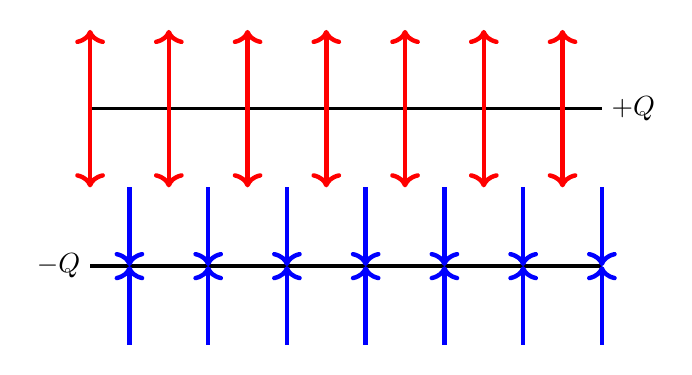
\begin{tikzpicture}
            \draw[very thick] (0, 0) -- (6.5, 0);
            \draw[very thick] (0, 2) -- (6.5, 2);
            \foreach \x in {0,...,6} {
                \begin{scope}[color=red, ultra thick]
                    \draw[->] (\x, 2) -- (\x, 1);
                    \draw[->] (\x, 2) -- (\x, 3);
                \end{scope}
                \begin{scope}[xshift=0.5cm, color=blue, ultra thick]
                    \draw[->] (\x, 1) -- (\x, 0);
                    \draw[->] (\x, -1) -- (\x, 0);
                \end{scope}
            }
            \node[right] at (6.5, 2) {\(+Q\)};
            \node[left] at (0, 0) {\(-Q\)};
        \end{tikzpicture}
        \caption{Parallel plate capacitor electric field.}
        \label{fig:parallel plate capacitor electric field}
    \end{figure}
    The potential difference between the fields is given by
    \[V = -\int_0^d E_z\dd{z} = \frac{\sigma}{\varepsilon_0}d = \frac{Qd}{A\varepsilon_0}\]
    where we have chosen a coordinate system such that \(\ve{z}\) is normal to the plates and points from the negative to the positive plate.
    The origin is also chosen to be in the negative plate.
    The area of each plate is \(A\).
    The capacitance is then given by
    \[C = \frac{Q}{V} = \frac{A\varepsilon_0}{d}.\]
    Notice that the capacitance depends only on the geometry of the plates (their area and the distance between) it is independent of the charge and potential difference.
    It turns out that in general capacitance is a purely geometric property.
    
    We can use the charge distribution to calculate the electrostatic energy of the charged capacitor.
    \begin{align*}
        U_E &= \frac{1}{2}Q(V_1 - V_2)\\
        &= \frac{1}{2}QV\\
        &= \frac{1}{2}\frac{Q^2}{E}
    \end{align*}
    We can also use the fact that the electric field vanishes outside of the plates to calculate the electrostatic energy of the charged capacitor.
    \begin{align*}
        U_E &= \frac{\varepsilon_0}{2}\int E^2\dd[3]{r}\\
        &= \frac{\varepsilon_0}{2} \left(\frac{\sigma}{\varepsilon_0}\right)^2 \int\dd[3]{r}\\
        &= \frac{\sigma^2}{2\varepsilon_0}dA\\
        &= \frac{dQ^2}{2\varepsilon_0A}\\
        &= \frac{1}{2}\frac{Q^2}{E}.
    \end{align*}
    Here we have used that the empty integral is just the volume which in this case since \(E = 0\) outside of the capacitor is just the volume between the plates, \(dA\).
    
    \subsubsection{Edge Effects}
    \textit{This section is non-examinable}
    
    So far we have assume that the plates are infinite and therefore the fields are uniform between the plates.
    However in reality the plates cannot be infinite.
    For a finite sized capacitor the field bulges out of the capacitor and isn't uniform between the plates.
    
    Suppose that instead of infinite planes the capacitor is made from two discs of radius \(R\).
    We can perform an integral over the charge distribution to obtain the potential a height \(z\) above the disc:
    \[V(z) = \frac{1}{4\pi\varepsilon_0}\int_S\frac{\sigma}{(\rho^2 + z^2)^{1/2}}\dd{S}.\]
    In plane polar coordinates \(\dd{S} = \rho\dd{\rho}\dd{\varphi}\) so
    \begin{align*}
        V(z) &= {\sigma}{4\pi\varepsilon_0} \int_{0}^{2\pi} \dd{\varphi} \int_0^R \dd{\rho} \frac{\rho}{(\rho^2 + z^2)^{1/2}}\\
        &= \frac{\sigma}{4\pi\varepsilon_0}2\pi\left[(\rho + z^2)^{1/2}\right]_{\rho=0}^{\rho=R}\\
        &= \frac{\sigma}{2\varepsilon_0}\left[(R^2 + z^2)^{1/2} - z\right].
    \end{align*}
    This means that the \(z\) component of the electric field is
    \[E_z = -\pdv{V}{z} = -\frac{\sigma}{2\varepsilon_0}\left[\frac{z}{(R^2 + z^2)^{1/2}} - 1\right].\]
    This depends on \(z\) so the field is not uniform between the plates.
    There are two interesting limiting cases.
    First \(R \ll z\):
    \begin{align*}
        \vv{E}(R) &= \frac{\sigma}{2\varepsilon_0}\left[1 - \left(1 + \frac{R^2}{z^2}\right)^{-1/2}\right]\ve{z}
        \shortintertext{Taylor expanding the binomial term gives}
        &\approx \frac{\sigma}{2\varepsilon_0}\left[1 - \left(1 - \frac{1}{2}\frac{R^2}{z^2}\right)\right]\ve{z}\\
        &= \frac{\sigma R^2}{4\varepsilon_0 z^2}\ve{z}\\
        &= \frac{Q}{4\pi\varepsilon_0 z^2}\ve{z}
    \end{align*}
    where \(Q = \sigma\pi R^2\) is the total charge.
    We see that in this limit we can essentially view the capacitors as a point charge when we are far enough away that we can approximate it as having no volume.
    
    The other interesting case is when \(R \gg z\).
    In this case the term \(z / (R^2 + z^2)^{-1/2}\approx 0\) so
    \[\vv{E}(R) = \frac{\sigma}{2\varepsilon_0}\ve{z}.\]
    So in the case that the discs are very large they approximate infinite planes.
    It is only when \(R\approx z\) (i.e. \(A\approx d^2\)) that we need to consider the edge effects of the capacitor.
    Fortunately in practice this is rarely necessary.
    \part{Magnetostatics}
    \section{The Magnetic Field}
    \subsection{The Magnetic Force}
    The \define{magnetic field}, \(\vv{B}\), is defined by the force, \(\vv{F}\), experienced by a charge, \(q\), with velocity \(\vv{v}\), in an external electric field \(\vv{E}\):
    \[\vv{F} = q(\vv{E} + \vv{v}\times\vv{B}).\]
    This is called the \define{Lorentz force law}.
    The units of \(\vv{B}\) are teslas, \si{\tesla}, defined by \(\SI{1}{\tesla} = \SI{1}{\newton.\ampere^{-1}.\metre^{-1}}\).
    This is quite a large unit and it is common to use an alternative unit called a gauss defined by \(\SI{e-4}{\tesla} = \SI{1}{\gauss}\) sometimes also denoted \(\SI{1}{\gaussAlternate}\).
    
    The important thing about this formula is that the force due to the magnetic field, \(\vv{v}\times\vv{B}\), is perpendicular to the velocity.
    This means that magnetic fields do no work as \(\vv{v}\cdot(\vv{v}\times\vv{B}) = \vv{0}\).
    
    \subsection{Current}
    A \define{current} is a moving density of charge.
    For a \define{steady current} at any point, \(\vv{r}\), a constant (time independent) density of charge moves past \(\vv{r}\) in a given time.
    Steady currents are important as if all currents are steady we will see that this leads to a constant magnetic field in the same way that stationary charges lead to a constant electric field.
    A current formed by \(n(\vv{r})\) charges, \(q\), moving past the point \(\vv{r}\) with average velocity \(\vv{v}(\vv{r})\) can be described by a \define{current density}
    \[\vv{J}(\vv{r}) = n(\vv{r})q\vv{v}(\vv{r}) = \rho(\vv{r})\vv{v}(\vv{r}).\]
    Here we have used \(n(\vv{r})q = \rho(\vv{r})\).
    The current density is to the magnetic field as the charge density is to the electric field.
    The units of \(\vv{J}\) are \(\si{\ampere.\metre^{-2}}\).
    We can similarly define a surface current density, usually denoted \(\vv{K}\) or \(\vv{j}\).
    This will have units of \(\si{\ampere.\metre^{-1}}\).
    We can also define a line current density, usually denoted \(\vv{I}\), which has units of \(\si{\ampere}\).
    
    The total current, \(I\), is the current density through a surface, \(A\):
    \[I = \int_A \vv{J}\cdot\dd{\vv{S}},\]
    where \(\dd{\vv{S}}\) is a surface element normal to \(A\).
    
    \begin{example}
        An insulating disc of radius \(R\) with uniform charge density, \(\sigma\), is rotated about its axis with an angular velocity, \(\vv{\omega} = \omega\ve{z}\).
        As a result the disc has a surface current density:
        \[\vv{K} = \sigma\vv{v} = \sigma\vv{\omega}\vv{r} = \sigma\omega\ve{z}\times r\ve{\rho} = \sigma\omega r\ve{\varphi}.\]
        Notice that this is a steady current even though the disc is moving faster towards the edge, hence scaling with \(r\).
        The important thing for a steady current is that the current is constant at any one point in space, not that it has the same value at all points of space.
    \end{example}
    
    \subsection{Conductivity}
    The \define{conductivity}, \(\sigma\), is an intrinsic bulk property of a material.
    It relates the current density to the electric field:
    \[\vv{J} = \sigma\vv{E}.\]
    This is \define{Ohm's law}.
    This assumes that \(\vv{J}\) and \(\vv{E}\) are parallel.
    This is only the case if the material is isotropic, that is all directions within the material are equivalent.
    If this isn't the case then we need to use the conductivity tensor, \(\sigma_{ij}\), instead.
    
    A typical value of \(\sigma\) for a metal is \(\SI{e9}{\ohm^{-1}.\metre^{-1}}\).
    We define the \define{resistivity} as
    \[\rho = \frac{1}{\sigma}.\]
    A typical value of \(\rho\) for an insulator is \(\SI{e16}{\ohm.\metre}\).
    In a superconductor \(\rho = 0\).
    
    Suppose a wire of cross sectional area \(A\) has a homogenous current density and electric field.
    The current in the wire is
    \[I = \int_A\vv{J}\cdot\dd{\vv{S}} = \int_A J\dd{S} = \int \sigma E\dd{S} = E\sigma A.\]
    The potential difference between two points on the wire a distance \(d\) apart is
    \[\Delta V = Ed.\]
    The current can then be written as
    \[I = \frac{A\sigma}{d}\Delta V.\]
    Rearranging we get
    \[\Delta V = IR,\qquad\text{where}\qquad R = \frac{d\rho}{A}.\]
    \(R\) here is what we define as the \define{resistance}.
    It has units of ohms, \(\si{\ohm}\).
    This equation is the more familiar form of Ohm's law.
    
    \subsection{Current Elements}
    A current element, \(\dd{\vv{\current}}\), is a vector defined by
    \begin{align*}
        \dd{\vv{\current}(\vv{r})} &= \vv{J}(\vv{r})\dd{V},\\
        \dd{\vv{\current}(\vv{r})} &= \vv{K}(\vv{r})\dd{S},\\
        \dd{\vv{\current}(\vv{r})} &= \vv{I}(\vv{r})\dd{l}.
    \end{align*}
    The units of a current element are \(\si{\ampere.\metre}\).
    Be careful, \(\vv{K}\dd{S} \ne K\dd{S}\), the first points in the direction of the surface current density, which is along the surface, and the second is normal to the surface.
    On the other hand \(\vv{I}\dd{l} = I\dd{\vv{l}}\) since a line current element always points along the line and so does a line element.

    A current is a moving charge element.
    For a bulk current density we have
    \[\dd{\vv{\current}}(\vv{r}) = \vv{J}(\vv{r})\dd{V} = \rho(\vv{r})\vv{v}(\vv{r})\dd{V} = \vv{v}(\vv{r})\dd{q}.\]
    This means that we can work out the force, \(\dd{\vv{F}}\), on a current element, \(\dd{\vv{\current}}\), in a magnetic field, \(\vv{B}\):
    \[\dd{\vv{F}} = \dd{q}\vv{v}\times\vv{B} = \dd{\vv{\current}}\times\vv{B}.\]
    If the current comes from a bulk current density, \(\dd{\vv{\current}} = \vv{J}\dd{V}\) then
    \[\dd{\vv{F}} = \vv{J}\times\vv{B}\dd{V}.\]
    
    \subsection{Biot Savart Law}
    The Biot Savart law is an empirical law relating current elements to the magnetic field.
    It states that if a current element \(\dd{\vv{\current}}(\vv{r'})\) is at position \(\vv{r'}\) then the resulting magnetic field at \(\vv{r}\) is given by
    \[\dd{\vv{B}(\vv{r})} = \frac{\mu_0}{4\pi} \frac{\dd{\vv{\current}(\vv{r'})} \times (\vv{r - \vv{r'}})}{\abs{\vv{r} - \vv{r'}}^3}.\]
    The Biot Savart law is to magnetic fields as Coulomb's law is to electric fields.
    It states that charge elements create magnetic fields which shows that a steady current causes a constant magnetic field.
    Here \(\mu_0\) is a constant known as the permeability of free space, or the electric constant.
    It has a value of
    \[\mu_0 = 4\pi\cdot\SI{e-7}{\henry.\metre^{-1}} = 4\pi\cdot\SI{e-7}{\newton.\ampere^{-2}}.\]
    Here \(\si{\henry}\) is a henry defined as \(\SI{1}{\henry} = \SI{1}{\newton.\metre.\ampere^{-2}}\).
    
    Since the Biot Savart law is linear in \(\dd{\vv{\current}}\) the superposition of the magnetic fields of many current elements to get the total magnetic fields holds so
    \[\vv{B}(\vv{r}) = \frac{\mu_0}{4\pi}\int \frac{\dd{\vv{\current}(\vv{r'})} \times (\vv{r} - \vv{r'})}{\abs{\vv{r} - \vv{r'}}^3}.\]
    For a bulk current density this becomes
    \[\vv{B}(\vv{r}) = \frac{\mu_0}{4\pi} \int \frac{\vv{J}(\vv{r'})\times(\vv{r} - \vv{r'})}{\abs{\vv{r} - \vv{r'}}^3} \dd[3]{r'}.\]
    
    \subsection{Magnetic Force Between Currents}
    The force on the current element \(\dd{\vv{\current_1}}\) at position \(\vv{r_1}\) due to a current element, \(\dd{\vv{\current_2}}\), at \(\vv{r_2}\) is
    \[\dd{\vv{F_1}} = \dd{\vv{\current_1}}\times\dd{\vv{B_2}} = \frac{\mu_0}{4\pi r_{12}^2} \dd{\vv{\current_1}} \times (\dd{\vv{\current_2}}\times \vhsub{r}{_{12}}).\]
    Here \(\dd{\vv{B_2}}\) is the magnetic field due to the second current element and \(\vv{r_{12}} = \vv{r_1} - \vv{r_2}\).
    If the each current element, \(\dd{\vv{\current_i}}\) is due to a bulk current density \(\vv{J_i}\) then this becomes
    \[\dd{\vv{F_1}} = \frac{\mu_0}{4\pi r_{12}^2} \vv{J_1}\times (\vv{J_2} \times \vhsub{r}{_{12}}) \dd[3]{r_1}\dd[3]{r_2}.\]
    
    \begin{example}
        A long straight wire is aligned along the \(z\)-axis.
        It carries a current, \(I\), in the positive \(z\) direction.
        What is the magnetic field strength at a point a distance \(r\) from the wire?
        
        A current element is given by
        \[\dd{\vv{\current}} = I\dd{z}\ve{z} = I\dd{\vv{r'}}\]
        where \(\vv{r'}\) is the position of the current element along the wire.
        Choosing the origin to be in the same plane as the point at which we are evaluating the field we have
        \[\vv{r} = \rho\ve{\rho}\]
        for the position at which we want to know the field strength (note that \(\rho\) here is cylindrical coordinates, not charge density or resistivity).
        Applying the Biot Savart law we get
        \begin{align*}
            \vv{B}(\vv{r}) &= \frac{\mu_0}{4\pi} \int \frac{\dd{\vv{\current}} \times (\vv{r} - \vv{r'})}{\abs{\vv{r} - \vv{r'}}^3}\\
            &= \frac{\mu_0}{4\pi} \int \frac{I\ve{z}\times(\rho\ve{\rho} - r'\ve{z})}{\abs{\vv{r} - \vv{r'}}^3} \dd{z}\\
            &= \frac{\mu_0}{4\pi} I \left[ \int \frac{\ve{z}\times\rho\ve{\rho}}{\abs{\vv{r} - \vv{r'}}^3} \dd{z} - \int \frac{\ve{z}\times r'\ve{z}}{\abs{\vv{r} - \vv{r'}}^3} \dd{z} \right]\\
            &= \frac{\mu_0 I}{4\pi}\rho\ve{\varphi}\int (\rho^2 + z^2)^{-3/2} \dd{z}\\
            &= \frac{\mu_0 I}{2\pi\rho}\ve{\varphi}.
        \end{align*}
        We looked up the integral in the last step over all \(z\in\reals\) and found it to be \(2/\rho^2\).
    \end{example}

    \section{Divergence and Curl of the Magnetic Field}
    \subsection{Divergence of the Magnetic Field}
    The Biot Savart law for a bulk current density, \(\vv{J}(\vv{r'})\), is
    \begin{align*}
        \vv{B}(\vv{r}) &= \frac{\mu_0}{4\pi} \int \vv{J}(\vv{r'}) \times \frac{(\vv{r} - \vv{r'})}{\abs{\vv{r} - \vv{r'}}^3} \dd[3]{r'}\\
        &= -\frac{\mu_0}{4\pi} \int \vv{J}(\vv{r'}) \times \grad_{\vv{r}}\left(\frac{1}{\abs{\vv{r} - \vv{r'}}}\right) \dd[3]{r'}
    \end{align*}
    Here we use a notation where differential operators with a subscript \(\vv{r}\) act only on the components of \(\vv{r}\).
    We can take the divergence of this fairly easily if we recognise that \(\vv{J}(\vv{r'})\) is constant with respect to \(\vv{r}\) so \(\grad_{\vv{r}}\cdot\vv{J}(\vv{r'}) = 0\).
    \begin{align*}
        \grad_{\vv{r}}\cdot\vv{B}(\vv{r}) &= -\frac{\mu_0}{4\pi} \int \grad_{\vv{r}}\cdot \left[\vv{J}(\vv{r'}) \times \grad_{\vv{r}}\left(\frac{1}{\abs{\vv{r} - \vv{r'}}}\right)\right] \dd[3]{r'}\\
        &= -\frac{\mu_0}{4\pi} \int \vv{J}(\vv{r'}) \cdot\left[\grad_{\vv{r}} \times \grad_{\vv{r}}\left(\frac{1}{\abs{\vv{r} - \vv{r'}}}\right)\right] \dd[3]{r'}\\
        &= 0
    \end{align*}
    Here we have used the identity that grad curl is zero.
    Hence
    \[\div\vv{B} = 0.\]
    This is \define{Maxwell's second law}.
    It states that there are no sinks or sources of the magnetic field,
    there are no magnetic monopoles, there are no point sources of the magnetic field, there are no `magnetic charges'.
    The magnetic field always forms closed loops.
    
    Applying the divergence theorem we have
    \[\int_V \div\vv{B}(\vv{r})\dd[3]{r} = \oint_A\vv{B}\cdot\dd{\vv{S}}.\]
    Identifying the left hand side as an integral of zero we have
    \[\oint_a\vv{B}\cdot\dd{\vv{S}} = 0.\]
    This is \define{Gauss' law for magnetic fields}.
    
    \subsection{Magnetic Dipoles}
    Maxwell's second law rules out the existence of magnetic monopoles.
    Therefore a magnetic dipole is the most elementary magnetic pole.
    It turns out that a magnetic dipole can be formed from a current loop.
    
    Suppose we have a circular loop or radius \(a\) carrying current \(I\).
    If we align the axis of the loop with the \(z\) axis so that the current is going in the \(\ve{\varphi}\) direction then the magnetic field on the axis can be found from the Biot Savart law,
    \[\dd{\vv{B}(\vv{r})} = \frac{\mu_0}{4\pi} \frac{\dd{\vv{\current}(\vv{r'})} (\vv{r} - \vv{r'})}{\abs{\vv{r} - \vv{r'}}^3}.\]
    Here \(\vv{r} = z\ve{z}\), \(\vv{r'} = a\ve{\rho}\), and \(\dd{\vv{\current}} = I\dd{\ell}\ve{\varphi}\).
    Hence
    \begin{align*}
        \dd{\vv{\current}} \times (\vv{r} - \vv{r'}) &= I\dd{\ell}\ve{\varphi} \times (z\ve{z} - a\ve{\rho})\\
        &= I\dd{\ell}(z\ve{\varphi}\times\ve{z} - a\ve{\varphi}\times\ve{\rho})\\
        &= I\dd{\ell}(z\ve{\rho} + a\ve{z}).
    \end{align*}
    Radial from diametrically opposed sides of the loop will cancel leaving a net field only in the \(\ve{z}\) direction:
    \[\dd{B_z} = \frac{\mu_0}{4\pi}\frac{Ia\dd{\ell}}{(a^2 + z^2)^{3/2}}\]
    Integrating this we get
    \begin{align*}
        B_z &= \frac{\mu_0}{4\pi} \frac{Ia}{(a^2 + z^2)^{3/2}} \oint\dd{\ell}\\
        &= \frac{\mu_0}{4\pi} \frac{Ia}{(a^2 + z^2)^{3/2}}2\pi a\\
        &= \frac{\mu_0Ia^2}{2(a^2 + z^2)^{3/2}}.
    \end{align*}
    At \(z = 0\) (i.e. the centre of the loop)
    \[B_z = \frac{\mu_0Ia^2}{2a^3} = \frac{\mu_0I}{2a}.\]
    In the far field (i.e. \(z \gg a\))
    \[B_z \approx \frac{\mu_0Ia^2}{2z^3}.\]
    It can be shown that off-axis field is
    \[\vv{B_{\mathrm{dip}}}(\vv{r}) = \frac{\mu_0}{4\pi r^3} [3(\vv{m}\cdot\vh{r})\vh{r} - \vv{m}]\]
    in the far field.
    Here \(\vv{m}\) is the dipole moment defined as
    \[\vv{m} = IA\ve{z}\]
    where \(A\) is the area of a current loop, in the \((x, y)\)-plane, and \(I\) is the current it carries.
    In this case \(A = \pi a^2\) so
    \[\vv{m} = I\pi a^2\ve{z}.\]
    More generally we can define the dipole moment as
    \[\vv{m} = I\vv{A} = I\int_A\dd{\vv{S}}\]
    where \(\vv{A}\) is the vector area of the loop defined by an integral over the entire loop, which may not be planar, and has surface elements \(\dd{\vv{S}}\).
    
    In an external magnetic field, \(\vv{B_\mathrm{ext}}\), a magnetic dipole has energy
    \[U = -\vv{m}\cdot\vv{B_\mathrm{ext}}.\]
    There is also a torque
    \[\vv{\tau} = \vv{m}\times\vv{B_\mathrm{ext}}.\]
    
    \subsection{Curl of the Magnetic Field}
    Starting again from the Biot Savart law for a bulk current density and this time taking the curl we have
    \[\grad_{\vv{r}} \times \vv{B}(\vv{r}) = -\frac{\mu_0}{4\pi} \int \grad_{\vv{r}} \times \left[\vv{J}(\vv{r'}) \times \grad_{\vv{r}}\left(\frac{1}{\abs{\vv{r} - \vv{r'}}}\right)\right] \dd[3]{r'}\]
    Looking just at the integrand we have
    \begin{align*}
        \grad_{\vv{r}} \times \left[\vv{J}(\vv{r'}) \times \grad_{\vv{r}}\left(\frac{1}{\abs{\vv{r} - \vv{r'}}}\right)\right] & = \vv{J}(\vv{r'})\laplacian_{\vv{r}}\left(\frac{1}{\abs{\vv{r} - \vv{r'}}}\right) - (\vv{J}(\vv{r'})\cdot\grad_{\vv{r}})\grad_{\vv{r}} \left(\frac{1}{\abs{\vv{r} - \vv{r'}}}\right)\\
        &= -4\pi\delta(\vv{r} - \vv{r'})\vv{J}(\vv{r'}) - (\vv{J}(\vv{r'})\cdot\grad_{\vv{r}}) \grad_{\vv{r}} \left(\frac{1}{\abs{\vv{r} - \vv{r'}}}\right).
    \end{align*}
    Hence the curl of the magnetic field is
    \begin{align*}
        \grad_{\vv{r}}\times\vv{B}(\vv{r}) &= \frac{\mu_0}{4\pi} \int 4\pi\delta(\vv{r} - \vv{r'})\vv{J}(\vv{r'}) \dd[3]{r'} + \frac{\mu_0}{4\pi} \int (\vv{J}(\vv{r'})\cdot\grad_{\vv{r}}) \grad_{\vv{r}} \left(\frac{1}{\abs{\vv{r} - \vv{r'}}}\right) \dd[3]{r'}
        \shortintertext{The second term can be shown to be zero by writing it as a boundary integral at infinity which must vanish to have finite energy}
        &= \frac{\mu_0}{4\pi} \int 4\pi\delta(\vv{r} - \vv{r'})\vv{J}(\vv{r'}) \dd[3]{r'}\\
        &= \mu_0\int \vv{J}(\vv{r'})\delta(\vv{r} - \vv{r'})\dd[3]{r'}\\
        &= \mu_0\vv{J}(\vv{r}).
    \end{align*}
    This is \define{Maxwell's fourth law}.
    Applying Stokes' theorem we have
    \[\int_S \curl\vv{B}\cdot\dd{\vv{S}} = \oint_C\vv{B}\cdot\dd{\vv{l}}.\]
    Looking at the left hand side we have
    \[\int_S \curl\vv{B}\cdot\dd{\vv{S}} = \mu_0 \int_S \curl\vv{J}\cdot\dd{\vv{S}} = \mu_0 I.\]
    Hence
    \[\oint_C\vv{B}\cdot\dd{\vv{l}} = \mu_0 I.\]
    This is \define{Ampere's law}.
    
    \begin{example}\label{exa:infinite wire magnetic field}
        Consider an infinite wire of radius \(a\) aligned along the \(\ve{z}\) direction carrying current density \(\vv{J}\propto\ve{z}\).
        We must have that \(B_z = 0\) as \(\vv{J}\) and \(\vv{B}\) must be perpendicular.
        Similarly we must have that \(B_\rho = 0\) as if there where radial components then \(\div\vv{B}\) would be non-zero violating the second of Maxwell's equations.
        Therefore \(\vv{B}\propto\ve{\varphi}\).
        Also \(B_\varphi\) cannot depend on \(z\) as we are free to place the origin anywhere along the wire and it cannot depend on \(\varphi\) as we are free to define any angle around the wire as \(\varphi = 0\).
        Thus we are left with
        \[\vv{B} = B_\varphi(\rho)\ve{\varphi}.\]
        For \(\rho > a\) we have
        \[\oint_C \vv{B}\cdot\dd{l} = B_\varphi 2\pi\rho = \mu_0 I_{\mathrm{enc}} = \mu_0 J\pi a^2.\]
        Hence
        \[B_\varphi = \frac{\mu_0 J}{2} \frac{a^2}{\rho}.\]
        For \(\rho < a\) we still have
        \[\oint_C \vv{B}\cdot\dd{\vv{l}} = B_\varphi 2\pi\rho\]
        but now
        \[\mu_0I_{\mathrm{enc}} = \mu_0J\pi\rho^2\]
        so
        \[B_\varphi = \frac{\mu_0J}{2}\rho.\]
        This is shown in figure~\ref{fig:magnetic field strength wire}.
        \begin{figure}[ht]
            \centering
            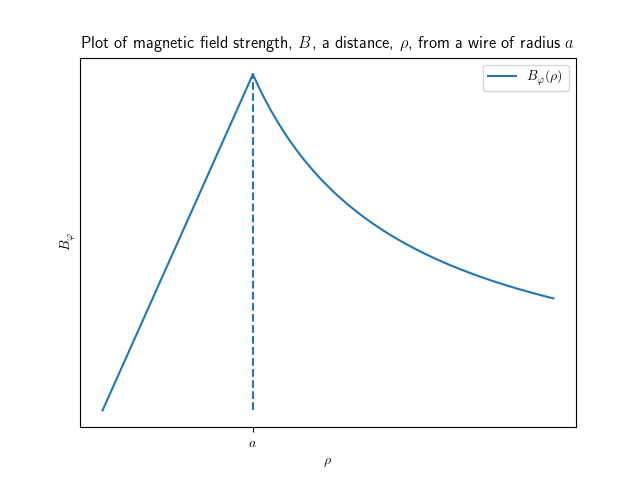
\includegraphics[scale=0.5]{magnetic_field_wire.png}
            \caption{The magnetic field strength a distance \(\rho\) from a wire.}
            \label{fig:magnetic field strength wire}
        \end{figure}
    \end{example}

    \section{Amp\`ere's Law and Vector Potentials}
    \subsection{Applications of Amp\`ere's Law}
    Amp\`ere's Law states
    \[\oint_C \vv{B}\cdot\dd{\vv{l}} = \mu_0 \int_A\vv{J}\cdot\dd{S} = \mu_0 I_\enc.\]
    Here \(\vv{B}\) is the magnetic field due to a current density \(\vv{J}\).
    \(C\) is some closed curve, called an Amp\`erian loop, bounding a surface \(A\) which has surface normals \(\dd{\vv{S}}\).
    \(I_\enc\) is the current that passes through the surface.
    The integration is performed along the curve in such a way that the surface normals and direction of integration agree with the right hand grip rule.
    Symmetry permitting Amp\`ere's law is usually the fastest way to calculate the magnetic field for a given current density.
    We look for cases where the Amp\`erian loop is either parallel or perpendicular to the magnetic field.
    The cases where this is possible and the Amp\`erian loops to use are
    \begin{itemize}
        \item Infinite straight line -- coaxial circles (see example~\ref{exa:infinite wire magnetic field})
        \item Infinite plane -- rectangular loop
        \item Infinite solenoid -- rectangular loop
        \item Toroid -- circle
    \end{itemize}
    \subsubsection{Infinite Slab of Current}
    An infinite slab of thickness \(d\) has a current density, \(\vv{J}\).
    Define the \(x\) direction to be the direction of this current density and the \(y\) direction to be in the slab but perpendicular to the current density and the \(z\) direction to be normal to the slab.
    
    The magnetic field cannot have an \(x\) component as the current density must be perpendicular to the magnetic field.
    The magnetic field cannot have a \(z\) component as if it did we could place a Gaussian surface with a section of the slab in it and the integral over it would be non-zero meaning that we would have non-vanishing divergence.
    This is forbidden by Maxwell's second law.
    This leaves us with a magnetic field that can only be in the \(y\) direction.
    
    If we choose to put the origin a distance \(d/2\) into the slab then since we can pick any point at this depth in the slab to place the origin we must have that \(B_y\) is independent of \(x\) and \(y\) and so \(B_y = B_y(z)\).
    
    We choose an Amp\`erian loop that is rectangular with two sides in the \(z\) direction and two in the \(y\) direction.
    The field is perpendicular to the sides in the \(z\) direction.
    The field is aligned with the sides in the \(y\) direction.
    Say that the length of these sides is \(b\), then
    \[\oint_C \vv{B}\cdot\dd{\vv{l}} = 2b\abs{B_y} = \mu_0I_\enc = \mu_0 bdJ\]
    \[\implies \abs{B_y} = \frac{1}{2}\mu_0 Jd.\]
    We know that \(\dd{\vv{\current}}\propto\ve{x}\) so for \(\vv{r}\propto\ve{z}\) we have, by the Biot Savart law, that
    \[\vv{B} \propto \vv{J}\times\vv{r} \propto \ve{x}\times\ve{z} = -\ve{y}\]
    This means that, outside of the slab, the magnetic field is
    \[
        \vv{B} =
        \begin{cases}
            -\frac{1}{2}\mu_0 Jd\ve{y}, & z > \frac{1}{2}d,\\
            +\frac{1}{2}\mu_0 Jd\ve{y}, & z < -\frac{1}{2}d.
        \end{cases}
    \]
    \begin{figure}[ht]
        \centering
        \tikzsetnextfilename{current-slab}
        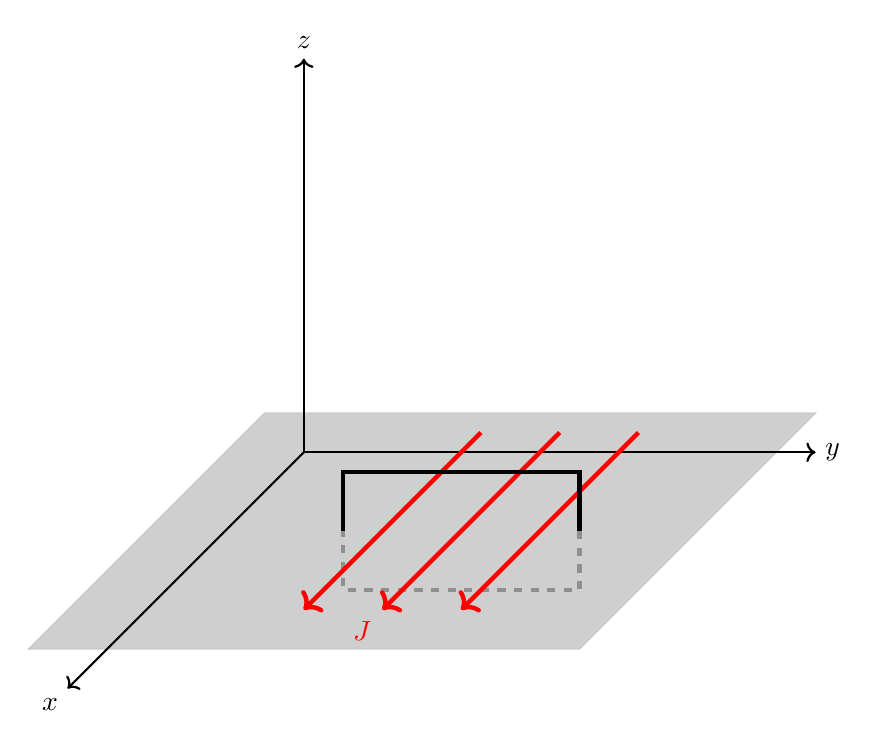
\begin{tikzpicture}
            \tikzstyle{current} = [color=red, ultra thick]
            \tikzstyle{axis} = [thick]
            \tikzstyle{conductor} = [color=lightgray, fill=lightgray, opacity=0.75]
            \tikzstyle{loop} = [ultra thick]
            \draw[dashed, loop] (3, -0.5) -- (3, -1.25) -- (0, -1.25) -- (0, -0.5);
            \draw[conductor] (-4, -2) -- (3, -2) -- (6, 1) -- (-1, 1) -- cycle;
            \begin{scope}[xshift=-0.5cm, yshift=0.5cm]
                \draw[axis, ->] (0, 0) -- (6.5, 0);
                \node[right] at (6.5, 0) {\(y\)};
                \draw[axis, ->] (0, 0) -- (0, 5);
                \node[above] at (0, 5) {\(z\)};
                \draw[axis, ->] (0, 0) -- (-3, -3);
                \node[below left] at (-3, -3) {\(x\)};
            \end{scope}
            \foreach \x in {0, 1, 2} {
                \draw[current, ->] (1.75 + \x, 0.75) -- (-0.5 + \x, -1.5);
            }
            \node[below left, current] at (0.5, -1.5) {\(\vv{J}\)};
            \draw[loop] (3, -0.5) -- (3, 0.25) -- (0, 0.25) -- (0, -0.5);
        \end{tikzpicture}
        \caption{Infinite slab of current}
    \end{figure}
    \begin{figure}[ht]
        \centering
        \tikzsetnextfilename{current-slab-2}
        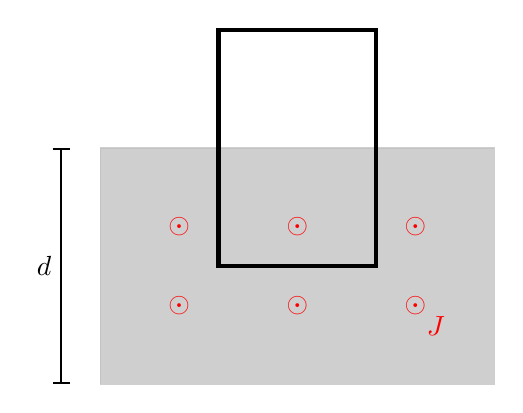
\begin{tikzpicture}
            \tikzstyle{current} = [color=red, ultra thick]
            \tikzstyle{conductor} = [color=lightgray, fill=lightgray, opacity=0.75]
            \tikzstyle{loop} = [ultra thick]
            \draw[conductor] (0, 0) rectangle (5, 3);
            %\draw (0, 0) grid (5, 3);
            \foreach \x in {1, 2.5, 4} {
                \foreach \y in {1, 2} {
                    \node[current] at (\x, \y) {\(\bm{\odot}\)};
                }   
            }
            \node[below right, current] at (4, 1) {\(\vv{J}\)};
            \draw[loop] (1.5, 1.5) rectangle (3.5, 4.5);
            \draw[thick, |-|] (-0.5, 0) -- (-0.5, 3);
            \node[left] at (-0.5, 1.5) {\(d\)};
        \end{tikzpicture}
        \caption{Finding the magnetic field inside a slab of current}
    \end{figure}
    If we want to know the magnetic field inside the slab then the set up for the Amp\'erian loop is similar but now one of the sides in the \(y\) direction should be inside the slab.
    We then use the field outside the loop that we already know to integrate along this loop.
    We find that
    \[B_{y,\text{in}} = -\mu_0Jz.\]
    \begin{figure}[ht]
        \centering
        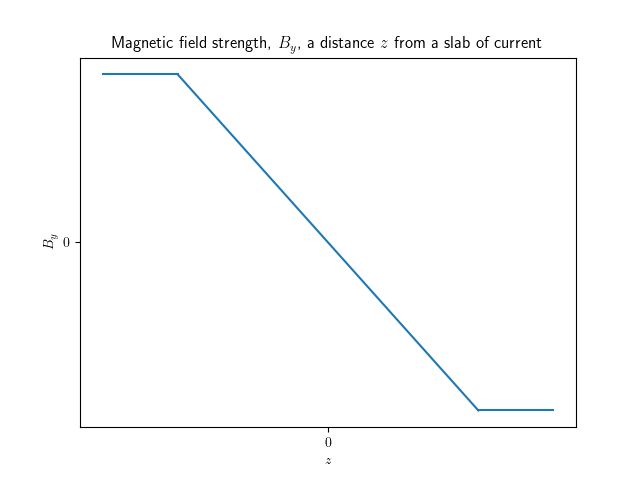
\includegraphics[scale=0.6]{magnetic_field_slab.png}
        \caption{The magnetic field strength, \(B_y\), a distance, \(z\), from a slab carrying current density, \(\vv{J}\).}
    \end{figure}

    \subsection{Toroid}
    A wire is curled up into a solenoid with \(n\) coils per unit length and radius \(R\).
    The solenoid is the curled up into a toroid of radius \(a > R\).
    \begin{figure}
        \centering
        \tikzsetnextfilename{toroid}
        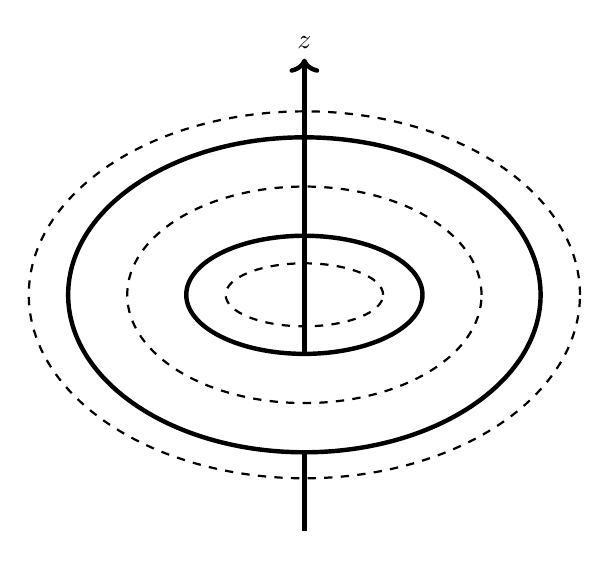
\begin{tikzpicture}
            \tikzstyle{axis} = [ultra thick]
            \tikzstyle{loop} = [thick, dashed]
            \tikzstyle{toroid} = [ultra thick]
            \draw[toroid] (0, 0) circle[x radius=3cm, y radius=2cm];
            \draw[toroid] (0, 0) circle[x radius=1.5cm, y radius=0.75cm];
            \draw[axis, ->] (0, -0.75) -- (0, 3);
            \draw[axis] (0, -2) -- (0, -3);
            \node[above] at (0, 3) {\(z\)};
            \draw[loop] (0, 0) circle[x radius=2.25cm, y radius=1.375cm];
            \draw[loop] (0, 0) circle[x radius=3.5cm, y radius=2.33cm];
            \draw[loop] (0, 0) circle[x radius=1cm, y radius=0.4cm];
        \end{tikzpicture}
        \caption{Finding the magnetic field inside a toroid}
        \label{fig:toroid}
    \end{figure}
    Figure~\ref{fig:toroid} shows a toroid (normal lines) with three possible Amp\'erian loops (dashed lines).
    The easiest loop to consider is the one that is entirely inside the hole of the toroid.
    Clearly there is no current enclosed in this so the magnetic field in the hole must be zero.
    Next we consider the outer most loop.
    At first it may seem like current does pass trough this but we must remember that the direction is important and therefore the \emph{net} current is zero as there is just as much current in both directions since the current is forming loops in the coil.
    Therefore outside of the toroid the magnetic field must be zero.
    The only Amp\'erian loop with a net current enclosed is the one that is in the toroid.
    
    All of the current element that pass through it are in the \((\rho, z)\)-plane, this means that \(\vv{B}\) can only be in the \(\ve{\varphi}\) direction.
    If the loop has radius \(\rho\) then we find that
    \[\oint_C\vv{B}\cdot\dd{\vv{l}} = 2\pi\rho B_\varphi = \mu_0I_\enc = \mu_0n2\pi aI\]
    where \(I\) is the current carried by the wire.
    Rearranging this we get
    \[B_\varphi = \frac{\mu_0nIa}{\rho}.\]
    
    \subsection{Magnetic Vector Potential}
    \begin{theorem}{}{}
        The following are equivalent for a vector field, \(\vv{B}\colon\reals^3 \to \reals^3\):
        \begin{enumerate}
            \item \(\div\vv{B} = 0\), in which case we call the field \define{solenoidal}.
            \item There exists a vector field, \(\vv{A}\colon\reals^3\to\reals^3\) such that \(\vv{B} = \curl\vv{A}\), in which case we call \(\vv{A}\) the \define{vector potential} of \(\vv{B}\).
            \item The surface integral
            \[\int_S\vv{B}\cdot\dd{\vv{S}}\]
            is independent of the shape of the surface, \(S\), for a given boundary curve.
            In particular
            \[\oint_S\vv{B}\cdot\dd{\vv{S}} = 0\]
            for any closed surface \(S\).
        \end{enumerate}
    \end{theorem}
    Maxwell's second equation tells us that \(\div\vv{B} = 0\) so there must exist \(\vv{A}\) such that
    \[\vv{B} = \curl\vv{A}.\]
    We call \(\vv{A}\) the \define{magnetic vector potential}.
    Compare this to the scalar electric potential, \(\varphi\) for a stationary electric field where we have
    \[\vv{E} = -\grad\varphi.\]
    
    \subsubsection{Poisson's Equation for the Vector Potential}
    Amp\`ere's law is
    \[\curl\vv{B} = \curl(\curl\vv{A}) = \mu_0\vv{J}.\]
    Applying a vector calculus identity we have
    \begin{equation}\label{eqn:curl A = laplacian A - grad div A = -mu0 J}
        -\curl(\curl\vv{A}) = \laplacian\vv{A} - \grad(\div\vv{A}) = -\mu_0\vv{J}.
    \end{equation}
    This is the most general form that we can find making no assumptions about the potential.
    However we have a \define{gauge freedom} that allows us to modify the potentials in a certain way without effecting the physics.
    That is the modified potentials given the same electric and magnetic fields.
    We have already seen this for the electric field.
    If we have two potentials, \(V(\vv{r})\) and \(\tilde{V}(\vv{r}) = V(\vv{r}) + C\) where \(C\in\reals\) then
    \[-\grad V(\vv{r}) = \vv{E}\]
    by definition but also
    \[-\grad\tilde{V} = -\grad(V + C) = -\grad V - \grad C = -\grad V = \vv{E}.\]
    Thus the field is unchanged by the addition of a constant to the potential.
    Similarly with the vector potential if we have two potentials, \(\vv{A}(\vv{r})\) and \(\vv{\tilde{A}}(\vv{r}) = \vv{A}(\vv{r}) + \grad\varphi(\vv{r})\) where \(\varphi\colon\reals^3\to\reals\) then
    \[\curl\vv{A} = \vv{B}\]
    by definition but also
    \[\curl\vv{\tilde{A}} = \curl(\vv{A} + \grad\varphi) = \curl\vv{A} + \curl\grad\vv{A} = \curl\vv{A} = \vv{B}.\]
    Thus the field is unchanged by the addition of a gradient field to the potential.
    
    We use this gauge freedom to select a gauge (a condition on the potential) that simplifies equations.
    One of the most common gauges to choose is the \define{Coulomb gauge}:
    \[\div\vv{A} = 0.\]
    For all magnetic fields, \(\vv{B}\), it is always possible to define a potential, \(\vv{A}\), such that
    \[\curl\vv{A} = \vv{B},\qquad\text{and}\qquad \div\vv{A} = 0.\]
    Given a potential \(\vv{A'}\) that satisfies the first of these condition then \(\vv{A} = \vv{A'} + \grad\varphi\) also satisfies the first condition.
    We can also require that
    \[\div\vv{A} = \div\vv{A'} + \div\grad\varphi = \div\vv{A} + \laplacian\varphi = 0 \implies \laplacian\varphi = -\div\vv{A}.\]
    This is simply \gls{pe} for \(\varphi\).
    We know that this has a solution
    \[\varphi(\vv{r}) = \frac{1}{4\pi}\int\frac{\div\vv{A}(\vv{r'})}{\abs{\vv{r} - \vv{r'}}^3}\dd[3]{r'}.\]
    
    In the Coulomb gauge equation~\ref{eqn:curl A = laplacian A - grad div A = -mu0 J} becomes
    \[\laplacian\vv{A} = -\mu_0\vv{J}.\]
    This is actually three equations, one for each component:
    \[\laplacian A_i - -\mu_0 J_i.\]
    So we have reduced equation~\ref{eqn:curl A = laplacian A - grad div A = -mu0 J} to \gls{pe} by carefully choosing a gauge.
    This means that we can use all of the methods we have already developed for \gls{pe}.
    In particular we have the explicit solution
    \[\vv{A}(\vv{r}) = \frac{\mu_0}{4\pi}\int\frac{\vv{J}(\vv{r'})}{\abs{\vv{r} - \vv{r'}}}\dd[3]{r'}.\]
    For example using this we can find that the magnetic dipole has a potential of
    \[\vv{A} = \frac{\,u_0}{4\pi}\frac{\vv{m}\times\vv{r}}{r^3}.\]
    
    \subsection{Summary of Statics}
    The electric field, \(\vv{E}\), and magnetic field, \(\vv{B}\), are defined such that for a charge, \(q\), moving at velocity \(\vv{v}\), the force on the charge is given by the Lorentz force law:
    \[\vv{F} = q(\vv{E} + \vv{v}\times\vv{B}).\]
    
    \subsubsection{Electrostatics}
    A static electric field is created by a stationary charge distribution, \(\rho\), meaning \(\partial_t\rho = 0\).
    The empirical law from which we derive everything else is Coulomb's law:
    \[\vv{F} = \frac{1}{4\pi\varepsilon_0}\frac{qQ}{r^2}.\]
    From this we can derive Maxwell's first and third laws, which are
    \[\div\vv{E} = \frac{\rho}{\varepsilon_0} \iff \oint_S\vv{E}\cdot\dd{\vv{S}} = \frac{Q_\enc}{\varepsilon_0},\tag{MI}\]
    and
    \[\curl\vv{E} = \vv{0} \iff \oint_C\vv{E}\cdot\dd{\vv{l}} = 0.\tag{MIII static}\]
    This last equation allows us to define an electrostatic potential, \(V\), such that
    \[\vv{E} = -\grad V.\]
    Combining this with Maxwell's first equation we get \gls{pe}:
    \[\laplacian V = -\frac{\rho}{\varepsilon}.\]
    
    \subsubsection{Magnetostatics}
    A static magnetic field is created by a steady current density, \(\vv{J}\), meaning \(\partial_t\vv{J} = \vv{0}\).
    The empirical law from which we derive everything else is the Biot Savart law:
    \[\dd{\vv{B}}(\vv{r}) = \frac{\mu_0}{4\pi}\frac{\dd{\vv{\current}}(\vv{r'})\times(\vv{r} - \vv{r'})}{\abs{\vv{r} - \vv{r'}}^3}.\]
    From this we can derive Maxwell's second and fourth laws, which are
    \[\div\vv{B} = 0 \iff \oint_S\vv{B}\cdot\dd{\vv{S}} = 0,\tag{MII}\]
    and
    \[\curl\vv{B} = \mu_0\vv{J} \iff \oint_C\vv{B}\cdot\dd{l} = \mu_0\int_S\vv{J}\cdot\dd{\vv{S}}.\tag{MIV static}\]
    The first of these allows us to define a vector potential, \(\vv{A}\), such that
    \[\vv{B} = \curl\vv{A}.\]
    Combining both of these equations, and working in the Coulomb gauge, \(\div\vv{A} = 0\), we get \gls{pe}:
    \[\laplacian\vv{A} = -\mu_0\vv{J}.\]
    \part{Electromagnetism}
    \section{Electromotance and Faraday's law}
    \subsection{Sources of Steady Current}\label{sec:sources of steady current}
    Consider a conducting loop where Ohm's law, \(\vv{J} = \sigma\vv{E}\), holds.
    Then integrating along the loop with Stokes' theorem we have
    \[\oint_C\vv{J}\cdot\dd{\vv{l}} = \sigma\oint_C\vv{E}\cdot\dd{\vv{l}} = \int_S\curl\vv{E}\cdot\dd{\vv{S}}.\]
    Here \(C\) is the loop and \(S\) is the disc it encloses.
    So far we have seen that \(\curl\vv{E} = \vv{0}\) and therefore we must have that \(\vv{J} = \vv{0}\).
    However this is clearly not true so \(\curl\vv{E} = \vv{0}\) must not always be correct.
    
    Similarly
    \[\oint_C\vv{J}\cdot\dd{\vv{l}} = \sigma\oint_C\vv{E}\cdot\dd{\vv{l}} = -\sigma\oint_C\grad V\cdot\dd{\vv{l}} = -\sigma [V(2\pi) - V(0)] = 0.\]
    Again this seems to imply that \(\vv{J} = \vv{0}\).
    The only assumption made here was that \(\vv{E} = -\grad V\) which is only valid if \(\curl\vv{E} = \vv{0}\).
    So it seems that \(\vv{E} = -\grad V\) also doesn't hold all the time.
    The question is what do we have to do to fix these equations so that they apply all the time.
    
    Imagine inserting a battery between the points \(B\) and \(A\) in the loop such that it creates a potential difference of \(\Delta V\).
    If we then integrate over the whole loop but \emph{not} the battery then we have
    \[\Delta V = \emf = \int_A^B \vv{E}\cdot\dd{\vv{l}}.\]
    Here \(\emf\) is known as the \define{electromotance}, or \define{\acrfull{emf}}.
    If we assume a unit test charge then we see that
    \[\emf = \oint\vv{F}\cdot\dd{\vv{l}}.\]
    
    \subsection{Induced EMF}
    We introduce here the \define{magnetic flux},
    \[\Phi_B = \int_A\vv{B}\cdot\dd{\vv{S}} = \oint_C\curl\vv{B}\cdot\dd{\vv{l}} = \oint_C\vv{A}\cdot\dd{\vv{l}}.\]
    
    Suppose a loop of wire is placed partly in a magnetic field as shown in figure~\ref{fig:induced emf in a loop moving through a magnetic field}.
    \begin{figure}[ht]
        \centering
        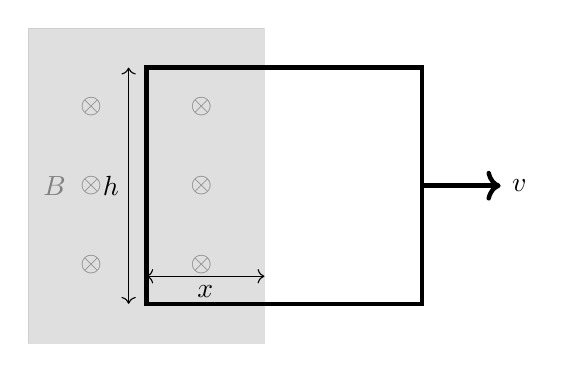
\begin{tikzpicture}
            \tikzstyle{magnetic field} = [color=lightgray, fill=lightgray, draw opacity=0.5, fill opacity=0.5]
            \tikzstyle{magnetic field label} = [color=gray]
            \tikzstyle{line} = [ultra thick]
            \draw[magnetic field] (0, 0) rectangle (3, 4);
            \foreach \x in {0.8, 2.2} {
                \foreach \y in {1, 2, 3} {
                    \node[magnetic field label] at (\x, \y) {\(\otimes\)};
                }
            }
            \node[magnetic field label, left] at (0.6, 2) {\(\vv{B}\)};
            \draw[line] (1.5, 0.5) rectangle (5, 3.5);
            \draw[line, ->] (5, 2) -- (6, 2) node[right] {\(\vv{v}\)};
            \draw[<->] (1.275, 0.5) -- (1.275, 3.5) node[midway, left] {\(h\)};
            \draw[<->] (1.5, 0.85) -- (3, 0.85) node[midway, below] {\(x\)};
        \end{tikzpicture}
        \caption{Wire loop moving through a magnetic field inducing an \gls{emf}.}
        \label{fig:induced emf in a loop moving through a magnetic field}
    \end{figure}
    The loop is dragged out of the field with a velocity \(\vv{v}\).
    The force on a charge carrier in the loop due to the magnetic field is given by
    \[\vv{F_M} = q\vv{v}\times\vv{B}.\]
    The \gls{emf} is
    \[\emf = \oint\vv{F_M}\cdot\dd{\vv{l}} = hvB.\]
    Here we have used that the force along the top and bottom parts of the loop are in opposite directions so cancel, meaning we only need to consider the contribution to the \gls{emf} of the force along the vertical section in the field.
    
    We can also calculate the magnetic flux:
    \[\Phi_B = \int\vv{B}\cdot\dd{\vv{S}} = Bhx\]
    where we define the surface normal so that the right hand rule with the current direction is satisfied.
    The flux is clearly not constant as the area of the loop that is in the field is changing:
    \[\dv{\Phi_B}{t} = \dv{t}Bhx = Bh\dv{x}{t} = -Bhx = -\emf.\]
    Note the minus sign as the area is decreasing.
    In fact the statement,
    \[\emf = -\dv{\Phi_B}{t},\]
    holds in general.
    This is called \define{Faraday's law of induction}.
    We say that this \gls{emf} is an induced \gls{emf} as it doesn't come from a normal source of \gls{emf} but rather the interaction of electric and magnetic fields.
    
    \subsection{Faraday's Law}
    Experimentally Faraday showed that altering \(\Phi_B\) by any of the following:
    \begin{enumerate}
        \item moving the surface,
        \item moving the field region,
        \item varying the field strength,
    \end{enumerate}
    produced an induced \gls{emf} in accordance with Faraday's law of induction.
    
    Note that in the last two of these the charges don't move so \(\vv{v} = 0\) meaning \(\vv{F_M} = \vv{0}\).
    Assuming that the Lorentz force law is correct there must be an induced electric field which creates a current.
    
    Faraday;s law has a differential form:
    \[\emf = -\dv{\Phi_B}{t} \implies \oint_C\vv{E}\cdot\dd{\vv{l}} = -\dv{t}\int_S\vv{B}\cdot\dd{\vv{S}}.\]
    Here \(C\) is the loop, \(S\) is the surface it encloses, and we have simply replaced \(\emf\) and \(\Phi_B\) with their definitions.
    We assume that the surface is constant so
    \[\dv{t}\int_S\vv{B}\cdot\dd{\vv{S}} = \int_S\partial_t\vv{B}\cdot\dd{\vv{S}}.\]
    We can also use Stokes' law to get
    \[\oint_C\vv{E}\cdot\dd{\vv{l}} = \int_S\curl\vv{E}\cdot\dd{\vv{S}}.\]
    Hence
    \[\int_S\curl\vv{E}\cdot\dd{\vv{S}} = -\int_S\partial_t\vv{B}\cdot\dd{\vv{S}}.\]
    Since both integrals are over the same area we must have that
    \[\curl\vv{E} = -\partial_t.\]
    We see that \(\curl\vv{E} = \vv{0}\) only holds for static magnetic fields.
    This is the full version of this law and is Maxwell's third equation.
    \[\emf = \oint_C\vv{E}\cdot\dd{\vv{l}} = -\dv{\Phi_B}{t} = -\dv{t}\int_S\vv{B}\cdot\dd{\vv{S}} \iff \curl\vv{E} = -\partial_t\vv{B}. \tag{MIII}\]
    
    \subsection{Connection to the Magnetic Vector Potential}
    If we combine \(\curl\vv{E} = -\partial_t\vv{B}\) and \(\vv{B} = \curl\vv{A}\) then we have
    \[\curl\vv{E} = -\partial_t(\curl\vv{A}) = -\curl(\partial_t\vv{A})\]
    which means
    \[\curl(\vv{E} - \partial_t\vv{A}) = \vv{0}.\]
    This means that there must exist a scalar field, \(V\), such that
    \[\vv{E} - \partial_t = -\grad V.\]
    Rearranging this we have
    \[\vv{E} = -\grad V - \partial_t\vv{A}.\]
    This is the most general way to write \(\vv{E}\) in terms of potentials, it reduces to \(\vv{E} = -\grad V\) if \(\vv{B}\) is time independent.
    We have now fixed the two equations that we showed weren't correct in section~\ref{sec:sources of steady current}.
    We see that there are two sources of the electric field:
    \begin{itemize}
        \item A stationary charge distribution, \(\rho\), which gives a contribution \(-\grad V\).
        \item A time dependent magnetic field, \(\vv{B}\), which gives a contribution \(-\partial_t\vv{A}\).
    \end{itemize}

    \subsection{Lenz's Law}
    \define{Lenz's law} is a rule of thumb that allows us to decide the sign of the flux.
    It states that the induced \gls{emf}, \(\emf\), acts in a way as to oppose the change that created it.
    For example in the case of removing a wire from a magnetic field the \gls{emf} causes a current in the wire in a direction such that the force due to the magnetic field's interaction with this current is in the opposite direction to the direction which the wire is being pulled.
    This is useful as it is often not that easy to see what the direction of the flux is and hence the direction of the induced \gls{emf} and induced current.
    
    \section{Induction}
    \subsection{Induction Examples}
    \subsubsection{AC Generator}
    A current loop, initially the \((x, z)\)-plane, with area \(A\) is placed in a uniform magnetic field, \(\vv{B}\).
    The loop is rotated at an angular velocity \(\vv{\omega} = \omega\ve{z}\).
    Since the loop is rotating the flux through the loop is time dependent:
    \[\Phi_B = \int_A\vv{B}\cdot\dd{\vv{S}} = B\cos(\omega t)\int_A\dd{S} = AB\cos(\omega t).\]
    Therefore there is an induced \gls{emf}:
    \[\emf = -\dv{\Phi_B}{t} = AB\omega\sin(\omega t).\]
    The induced current will be an AC current with a frequency \(\omega\).
    The current is \(\pi/2\) out of phase with the flux in a way that means that the peak current occurs when the flux is zero.
    
    \subsubsection{Rotating Disc of Charge}
    An insulating disc of radius \(a\) with a uniform surface charge density, \(\sigma\), is rotated around its axis.
    There is a uniform magnetic field parallel to the axis of the disc.
    The magnetic force on a charge element, \(\dd{q}\), on the disc at a radius \(r\), is
    \[\dd{\vv{F}} = \dd{q}vB\ve{\rho} = \dd{q}r\omega B\ve{\rho}.\]
    This magnetic force is equivalent to a radial electric field:
    \[\vv{E'} = \frac{1}{q}\vv{F} = r\omega B\ve{\rho}.\]
    The induced \gls{emf} between the centre and edge of the disc is then
    \[\emf = \int_{0}^a\vv{E'}\cdot\ve{\rho}\dd{\rho} = \frac{\omega Ba^2}{2}.\]
    This acts outwards to move the charge to the outside of the disc.
    If the disc were a conductor then this would actually happen.
    
    While the flux rule,
    \[\emf = -\dv{\Phi_B}{t},\]
    is still valid there is not a useful current loop to compute the flux through so it isn't of much help in this problem.
    
    \subsection{Mutual Inductance}
    Two current loops, \(C_1\) and \(C_2\) are carrying currents \(I_1\) and \(I_2\) in directions \(\dd{\vv{l_1}}\) and \(\dd{\vv{l_2}}\) respectively at positions \(\vv{r_1}\) and \(\vv{r_2}\).
    Current \(I_1\) creates a magnetic field, \(\vv{B_1}\), which passes through loop 2.
    Therefore a current is induced in loop 2.
    The induced flux in loop 2 is
    \[\Phi_2 = \int_{S_2}\vv{B_1}\cdot\dd{\vv{S_2}} = M_{21}I_1\]
    where we have used that \(\abs{\vv{B_1}}\propto I_1\) and \(M_{21}\) is just a constant of proportionality called the \define{mutual inductance}.
    If we substitute the vector potential, \(\vv{A_1}\), such that \(\vv{B_1} = \curl\vv{A_1}\), we get
    \begin{align*}
        \Phi_2 &= \int_{S_2} \vv{B_1}\cdot\dd{\vv{S_2}}\\
        &= \int_{S_2} (\curl\vv{A_1})\cdot\dd{\vv{S_2}}\\
        &= \oint_{C_2} \vv{A_1}\cdot\dd{\vv{l_1}}\\
        &= \frac{\mu_0 I_1}{4\pi} \oint_{C_2}\oint_{C_1} \frac{\dd{\vv{l_1}}\cdot\dd{\vv{l_2}}}{\abs{\vv{r_1} - \vv{r_2}}}.
    \end{align*}
    In the last step we have used the explicit solution to \gls{pe}, \(\laplacian\vv{A} = -\mu_0\vv{J}\).
    This gives us that
    \[M_{21} = \frac{\mu_0}{4\pi}\oint_{C_2}\oint_{C_1} \frac{\dd{\vv{l_1}}\cdot\dd{\vv{l_2}}}{\abs{\vv{r_1} - \vv{r_2}}}.\]
    This is called the Neumann formula.
    It isn't that useful, as it is pretty hard to calculate for arbitrary geometries, it is important to note that it is symmetric in 1 and 2, that is if we perform the equivalent calculation but completely swap the two loops we will get the same answer so
    \[M_{21} = M_{12} = M.\]
    The flux through loop 1 due to a current \(I\) in loop 2 is the same as the flux through loop 2 due to a current \(I\) in loop 1.
    
    The induced \gls{emf} in loop 2 due to current \(I_2\) is
    \[\emf_2 = -\dv{\Phi_2}{t} = -\dv{t}[MI_1] = -M\dv{I_1}{t}.\]
    We can then use Lenz's law to calculate the direction of the current noting that it must oppose any change in \(I_1\).
    
    One application of this is a spark plug in a car.
    In this loop 1 is wrapped around a core a few times and loop 2 is wrapped around the same core many many times.
    This leads to a very large value of \(M\) and so a small current in loop 1 can create a very large current in loop 2 which is large enough to spark across an air gap and ignite the fuel.
    
    \subsection{Self Inductance}
    If a loop carries a current then it generates a magnetic field.
    This magnetic field creates a flux through the loop.
    Therefore if the current is time dependent there will be an induced \gls{emf} and induced current in the loop that acts to oppose the change in the initial current.
    The \gls{emf} will be
    \[\emf = -\dv{\Phi_B}{t} = -L\dv{I}{t},\]
    where we have defined \(L\), the \define{self inductance}, to be such that \(\Phi_B = LI\).
    
    For example a solenoid of length \(\ell\) and radius \(a\) with \(n\) loops per unit length has an interior magnetic field of
    \[\vv{B} = B_z\ve{z} = \mu_0 nI\ve{z}.\]
    Each loop is approximately a closed circle of area \(A = \pi a^2\) and so the total flux through all \(n\ell\) loops is
    \[\Phi_B = \int \vv{B}\cdot\dd{\vv{S}} = An\ell B_z = \mu_0I\pi a^2n^2\ell.\]
    We can then identify the self inductance as
    \[L = \mu_0 \pi a^2n^2\ell = \mu_0n^2V_s\]
    where \(V_s = \pi a^2\ell\) is the volume of the solenoid.
    
    \subsection{Electronics}
    \textit{This section is non-examinable}
    
    We have introduced three material properties which all relate a voltage, \(\Delta V\), to the charge, \(Q\), in a different way:
    \begin{itemize}
        \item Resistance, \(R\):
        \[\Delta V \sim I \sim \dv{Q}{t}.\]
        \item Capacitance, \(C\):
        \[\Delta V\sim Q.\]
        \item Inductance, \(L\):
        \[\Delta V \sim \dv{I}{t} \sim \dv[2]{Q}{t}.\]
    \end{itemize}
    By constructing a circuit with two of these in series we can model differential equations.
    Since they are in series the voltage in all components will be the same.
    We start with a resistor and capacitor.
    From the fact that the voltages are equal we have that
    \[\dv{Q}{t} \sim Q \implies Q = Q_0e^{-\alpha t}\]
    for some constants \(Q_0\) and \(\alpha\).
    If we swap the capacitor for an inductor then we will have
    \[\dv{I}{t} \sim I \implies I = I_0e^{-\beta t}\]
    for some constants \(I_0\) and \(\beta\).
    Finally if we have a capacitor and inductor in series then
    \[\dv[2]{Q}{t} \sim Q \implies Q = Q_0'\sin(\omega t + \varphi) \implies I = Q_0'\omega\cos(\omega t + \varphi)\]
    for some constants \(Q_0'\), \(\omega\), and \(\varphi\).
    
    In the first case the charge on the capacitor decays away exponentially.
    In the second case the current that is initially induced by the inductor decays away exponentially.
    In the last case if initially we start with a charged capacitor and with no current (\(\varphi = \pi/2\)) then as the capacitor discharges a current is is induced and this charges the capacitor and we get an oscillating charge and current.
    
    \subsection{Magnetic Energy in Inductors}\label{sec:energy magnetic field}
    In electrostatics the electrostatic energy is due to the work done to create a charge distribution, done against Coulomb repulsion.
    Similarly in magnetostatics the magnetostatic energy is due to the work done to create a steady current, done against the induced \gls{emf} which opposes the creation of any current.
    
    If we try to create a current, \(\dd{I}\), in a loop in time \(\dd{t}\) we need to do work against the induced \gls{emf}, \(\emf\):
    \[\dd{U_M} = -\emf I\dd{t} = LI\dv{I}{t}\dd{t} = LI\dd{I},\]
    where \(L\) is the self inductance of the loop and we have used that
    \[-\emf = \dv{\Phi_B}{t} = \dv{t}[LI] = LI\dv{I}{t}.\]
    Integrating the energy with time we get
    \[U_M = \frac{1}{2}LI^2.\]
    Compare this to the equivalent statement in electrostatics that
    \[U_E = \frac{1}{2}\frac{Q^2}{C}.\]
    For two loops with inductances \(L_1\) and \(L_2\) carrying currents \(I_1\) and \(I_2\) with mutual inductance \(M\) then the energy becomes
    \[U_M = \frac{1}{2}L_1I_1^2 + \frac{1}{2}L_2I_2^2 + MI_1I_2.\]
    We can generalise the energy to any current arrangement:
    \begin{align*}
        U_M = \frac{1}{2}LI^2\\
        &= \frac{1}{2}\Phi_BI\\
        &= \frac{1}{2}I\oint_C \vv{A}\cdot\dd{\vv{l}}\\
        &= \frac{1}{2}\oint_C \vv{A}\cdot\vv{I}
    \end{align*}
    for a single loop.
    Notice that \(\oint_C \vv{A}\cdot\vv{I}\) is effectively a volume integral over all space of \(\vv{J}\) since this is only non-zero where there is a current, which in the case of a single loop reduces to a contour integral.
    Hence
    \[U_M = \frac{1}{2}\int\vv{A}\cdot\vv{J}\dd{V}.\]
    Where the integral is performed over all space.
    Using Amp\`ere's law we have
    \begin{align*}
        \mu_0\vv{A}\cdot\vv{J} &= \vv{A}\cdot(\curl\vv{B})\\
        &= \abs{\vv{B}}^2 - \div(\vv{A}\times\vv{B})
    \end{align*}
    where we have used the vector identity
    \begin{align*}
        \div(\vv{A}\times\vv{B}) &= \vv{B}\cdot\underbrace{(\curl\vv{A})}_{=\vv{B}} - \vv{A}\cdot(\curl\vv{B})\\
        &= \vv{B}\cdot\vv{B} - \vv{A}\cdot(\curl\vv{B})\\
        &= \abs{\vv{B}}^2 - \vv{A}\cdot(\curl\vv{B}).
    \end{align*}
    Hence the energy is
    \[U_M = \frac{1}{2}\vv{A}\cdot\vv{J}\dd{V} = \frac{1}{2\mu_0}\int\abs{\vv{B}}^2\dd{V} - \frac{1}{2\mu_0}\int\div(\vv{A}\times\vv{B})\dd{V}.\]
    We can write this last integral as a surface integral using the divergence theorem:
    \[\int\div(\vv{A}\times\vv{B})\dd{V} = \oint_S(\vv{A}\times\vv{B})\cdot\dd{\vv{S}}.\]
    If \(A\sim 1/r\) and \(B\sim 1/r^2\), as is the case for steady, finite, localised currents, then \(\abs{\vv{A}\times\vv{B}}\sim 1/r^3\).
    The surface area, \(S\sim r^2\).
    Since the volume integral is over all space the surface integral is over a boundary at infinity and so
    \[\int(\vv{A}\times\vv{B})\cdot\dd{\vv{S}} \sim \frac{1}{r^3}r^2 = \frac{1}{r}\]
    which becomes zero as \(r\to\infty\).
    Hence the energy is
    \[U_M = \frac{1}{2\mu_0}\int\abs{\vv{B}}^2\dd{V}.\]
    We can define an energy density, \(u_M\), such that
    \[u_m = \frac{\abs{\vv{B}}^2}{2\mu_0} \implies U_M = \int u_m\dd{V}.\]
    Compare this to the electrostatic case
    \[u_E = \frac{1}{2}\varepsilon\abs{\vv{E}}^2.\]
    
    \section{Displacement Current}
    \subsection{The Continuity Equation}
    The global electric charge is conserved.
    This means that the only way that the charge contained in a volume, \(V\), can change is if charge enters or leaves the volume.
    In the case that this happens there will be a current \(\vv{J}\) associated with the charge moving.
    The charge enters the volume at a rate of
    \[\pdv{Q}{t} = -\oint_S\vv{J}\cdot\dd{\vv{S}}.\]
    The minus sign accounts for the fact the surface normal, \(\dd{\vv{S}}\), points out of the volume so \(\vv{J}\cdot\dd{\vv{S}}\) is the charge leaving the volume through the surface \(\dd{\vv{S}}\), on the other hand \(\partial_t\) is the rate of increase of charge.
    Substituting in the charge density and applying the divergence theorem we have
    \[-\pdv{t}\int_{V}\rho\dd{V} = \int_V \div\vv{J}\dd{V}.\]
    Since this holds for all volumes we must have
    \[-\pdv{\rho}{t} = -\div\vv{J}.\]
    This is the \define{continuity equation}.
    It actually applies to any conserved quantity with an associated density and current.
    For example if \(\rho\) is mass density and \(\vv{J}\) is mass current which describes how mass is moving, for example it may describe fluid flow, then the continuity equation applies.
    Another important application is in quantum mechanics where \(\rho\) is the probability density and \(\vv{J}\) is a probability current which describes how the probability of different states changes with time.
    
    \subsection{Displacement Current}
    Amp\`ere's law is
    \[\curl\vv{B} = \mu_0\vv{J}.\]
    Taking the divergence of this we have
    \[\div(\curl\vv{B}) = \mu_0\div\vv{J}.\]
    The left hand side is identically zero by a vector calculus identity.
    For the right hand side we apply the continuity equation and get
    \[0 = -\mu_0\pdv{\rho}{t}.\]
    This is obviously wrong for a non-static charge distribution, \(\rho(\vv{r}, t)\), which we know can exist and would expect \(\rho\) not to be constant with time.
    Using the continuity equation we can known
    \[\div\vv{J} + \pdv{\rho}{t} = 0\]
    and so
    \[\div(\curl\vv{B}) = \mu_0(\div\vv{J} + \partial_t\rho)\]
    From Maxwell's first law we know that
    \[\rho = \varepsilon_0\div\vv{E}\]
    so
    \[\div(\curl\vv{B}) = \mu_0(\div\vv{J} + \varepsilon_0\partial_t\div\vv{E}) = \mu_0 \div(\vv{J} + \varepsilon_0\partial_t\vv{E})\]
    Since \(\div(\curl\vv{K}) = 0\) for all vector fields, \(\vv{K}\), we must have
    \[\curl\vv{B} = \mu_0(\vv{J} + \varepsilon_0\partial_t\vv{E} + \curl\vv{K}).\]
    It turns out that \(\vv{K} = \vv{0}\), this is required so that in the static case this equation reduces to \(\curl\vv{B} = \mu_0\vv{J}\).
    Therefore
    \[\curl\vv{B} = \mu_0(\vv{J} + \varepsilon_0\partial_t\vv{E}).\]
    This is the \define{Amp\`ere--Maxwell law} and is the full version of Maxwell's fourth equation with time dependent fields.
    It also has an integral form, using Stoke's theorem we have
    \[\int_S(\curl\vv{B})\cdot\dd{\vv{S}} = \oint_C \vv{B}\cdot\dd{\vv{l}}\]
    also
    \[\mu_0\int_S \vv{J}\cdot\dd{\vv{S}} + \varepsilon_0\int_S \pdv{t}\vv{E}\cdot\dd{\vv{S}} = \mu_0\int_S \vv{J}\cdot\dd{\vv{S}} + \mu_0\varepsilon_0\dv{t}\int\vv{E}\cdot\dd{\vv{S}}\]
    so
    \[\oint_C\vv{B}\cdot\dd{\vv{l}} = \mu_0\int_S \vv{J}\cdot\dd{\vv{S}} + \mu_0\varepsilon_0\dv{t}\int\vv{E}\cdot\dd{\vv{S}}\]
    What this law tells us is that magnetic fields can originate from two sources:
    \begin{itemize}
        \item Steady currents, \(\vv{J}\)
        \item Time dependent electric fields, \(\vv{E}\) (which themselves are created by time dependent charge densities or time dependent magnetic fields that change at a non-constant rate).
    \end{itemize}
    We call \(\varepsilon_0\partial_{t}\vv{E}\) the \define{displacement current} because it has dimensions of current density and creates a magnetic field.
    It is not a real current however.
    
    \subsubsection{Capacitor Paradox and Resolution}
    The capacitor paradox is another example of why Amp\`ere's law alone is not quite correct.
    The capacitor paradox is as follows.
    Consider a capacitor charging/discharging with a time dependent current, \(I(t)\),
    What is the magnetic field?
    Since the current is time dependent then so is the field.
    By Amp\`ere's law we have
    \[\oint_C\vv{B}\cdot\dd{\vv{l}} = \mu_0\int_S\vv{J}\cdot\dd{\vv{S}}.\]
    The paradox arises in the right hand side of this equation.
    If we take the surface \(S\) to cut through the wire then the right hand side is equal to \(\mu_0I(t)\).
    It is also possible to construct a surface with the same boundary in a way such that the surface goes in between the plates of the capacitor without ever intersecting any of the circuit.
    Then the right hand side of this equation is zero.
    
    We fix the supposed paradox by using the full Amp\`ere--Maxwell law.
    We known that for an ideal parallel plate capacitor the electric field is entirely constrained to be between the plates and in this volume it is normal to the plates and the field strength is
    \[E(t) = \frac{Q(t)}{\varepsilon_0 A}\]
    where \(A\) is the area of the plates.
    If we define the direction of \(\vv{E}\) to be the \(z\) direction then
    \[\varepsilon_0\partial_t\vv{E} = \frac{1}{A}\pdv{Q}{t}\ve{z} = \frac{I(t)}{A}\ve{z}.\]
    If we also choose to construct the surface so that it is parallel to the plates of the capacitor when it is between them then
    \[\mu_0\int_{S_2}(\vv{J} + \varepsilon_0\partial_t\vv{E})\cdot\dd{\vv{S}} = \frac{I(t)}{A}\int_{S_2}\dd{S} = \mu_0I(t)\]
    where we have used the fact that the field is zero outside of the capacitors so the surface integral is equivalent to an integral over the area of the capacitor.
    This is exactly the same result that we get using the other surface so we have fixed the paradox.
    \begin{figure}[ht]
        \centering
        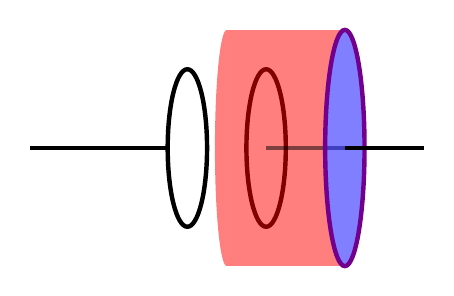
\begin{tikzpicture}
            \tikzstyle{line} = [ultra thick]
            \draw[line] (0, 0) -- (1.75, 0);
            \draw[line] (2, 0) circle[x radius=0.25cm, y radius=1cm];
            \draw[line] (3, 0) circle[x radius=0.25cm, y radius=1cm];
            \fill[color=red, opacity=0.5] (2.5, -1.5) rectangle (4, 1.5);
            \begin{scope}
                \clip (2.5, -1.5) rectangle (0, 1.5);
                \fill[color=red, opacity=0.5] (2.5, 0) circle[x radius=0.15cm, y radius=1.5cm];
            \end{scope}
            \draw[color=red, opacity=0.25] (2.5, -1.5) -- (2.5, 1.5);
            \fill[white] (4, 0) circle[x radius=0.25cm, y radius=1.5cm];
            \draw[line, opacity=0.5] (3, 0) -- (5, 0);
            \fill[color=blue, opacity=0.5] (4, 0) circle[x radius=0.25cm, y radius=1.5cm];
            \draw[color=red!45!blue, line] (4, 0) circle[x radius=0.25cm, y radius=1.5cm];
            \draw[line] (4, 0) -- (5, 0);
        \end{tikzpicture}
        \caption{The capacitor paradox. The two surfaces used in the capacitor paradox. \(S_1\) in blue goes through the wire and \(S_2\) in red goes through the gap in the capacitor. They share the boundary, \(C\), shown in purple.}
    \end{figure}
    
    \subsection{Maxwell's Equations}
    Maxwell's equations in differential form are
    \begin{align*}
        \div \vv{E} &= \frac{\rho}{\varepsilon_0},\tag{MI}\\
        \div \vv{B} &= 0,\tag{MII}\\
        \curl\vv{E} &= -\partial_t\vv{B},\tag{MIII}\\
        \curl\vv{B} &= \mu_0(\vv{J} + \varepsilon_0\partial_t\vv{E}).\tag{MIV}\\
    \end{align*}
    In integral form these are
    \begin{align*}
        \oint_S \vv{E}\cdot\dd{\vv{S}} &= \frac{Q_\enc}{\varepsilon_0}, \tag{MI}\\
        \oint_S \vv{B}\cdot\dd{\vv{S}} &= 0, \tag{MII}\\
        \oint_C \vv{E}\cdot\dd{\vv{l}} &= -\dv{t}\int_S \vv{B}\cdot\dd{\vv{S}} = -\dv{\Phi_B}{t} = \emf, \tag{MIII}\\
        \oint_C \vv{B}\cdot\dd{\vv{l}} &= \mu_0\int_S\vv{J}\cdot\dd{\vv{S}} + \mu_0\varepsilon_0\dv{t}\int_S \vv{E}\cdot\dd{\vv{S}} = \mu_0I_{\enc} + \mu_0\varepsilon_0\dv{\Phi_E}{t}. \tag{MIV}
    \end{align*}
    The first two equations are Gauss' laws for electric and magnetic fields, the third is Faraday's law of induction and the fourth is the Amp\`ere--Maxwell law.
    Combining Maxwell's first and fourth laws as well as the fact that the divergence of a curl is zero we get
    \[0 = \div(\curl\vv{B}) = \mu_0\left[\div\vv{J} + \varepsilon_0 \partial_t\div\vv{E} \right] = \mu_0\left[\div\vv{J} + \partial_t\rho\right]\]
    which is the continuity equation again.
    \subsubsection{Solutions to Maxwell's Equation}
    We will look for non-trivial solutions to Maxwell's equations in free space, that is with \(\rho = 0\) and \(\vv{J} = \vv{0}\).
    In this case Maxwell's equations become
    \begin{align*}
        \div\vv{E} &= 0\tag{MI in free space}\\
        \div\vv{B} &= 0\tag{MII}\\
        \curl\vv{E} &= -\partial_t\vv{B}\tag{MIII}\\
        \curl\vv{B} &= \mu_0\varepsilon_0\partial_t\vv{E}\tag{MIV in free space}
    \end{align*}
    Taking the curl of the third equation we have
    \[\curl(\curl\vv{E}) = -\curl(\partial_t\vv{B}) = -\partial_t\curl\vv{B} = -\mu_0\varepsilon_0\partial_t^2\vv{E}.\]
    Similarly taking the curl of the fourth equation we have
    \[\curl(\curl\vv{B}) = \mu_0\varepsilon_0\curl(\partial_t\vv{E}) = \mu_0\varepsilon_0\partial_t\curl\vv{E} = -\mu_0\varepsilon_0\partial_t^2\vv{B}.\]
    Or we can use the vector identity
    \[\curl(\curl\vv{K}) = \grad(\div\vv{K}) - \laplacian\vv{K}\]
    and we get
    \[\curl(\curl\vv{E}) = \grad(\div\vv{E}) - \laplacian\vv{E} = -\laplacian\vv{E},\]
    and
    \[\curl(\curl\vv{B}) = \grad(\div\vv{B})  -\laplacian\vv{B} = -\laplacian\vv{E}.\]
    Thus
    \[\partial_t^2\vv{E} = \frac{1}{\mu_0\varepsilon_0}\laplacian\vv{E}\qquad\text{and}\qquad \partial_t^2\vv{B} = \frac{1}{\mu_0\varepsilon_0}\laplacian\vv{B}.\]
    Thus we have turned four coupled first order \glspl{pde} into two seemingly uncoupled second order \glspl{pde}.
    They are only seemingly uncoupled as Maxwell's laws always apply.
    We can identify these equations as wave equations, which have the general form
    \[\partial_t^2\vv{u} = v^2\laplacian\vv{u}\]
    where \(v\) is the speed of waves in the vector field \(\vv{u}\).
    We see that for the waves in the electric and magnetic fields
    \[v = \frac{1}{\sqrt{\mu_0\varepsilon_0}} = c\]
    and indeed these equations relate to electromagnetic waves.
    
    \section{Electromagnetic Waves}
    \subsection{The Wave Equation in One Dimension}
    The wave equation for a scalar field, \(u\), with a wave propagating at speed \(c\), is
    \[\pdv[2]{u}{x} = \frac{1}{c^2}\pdv[2]{u}{t}.\]
    This is a second order \gls{pde} and typically we have initial conditions of \(u(x, 0)\) and \(\dot{u}(x, 0)\).
    Any twice differentiable function, \(u\), of the form
    \[u(x, t) = f(kx - \omega t),\]
    or equivalently
    \[u(x, t) = g(x - ct),\]
    satisfies this equation and represents a wave moving in the \(x\) direction at speed
    \[c = \frac{\omega}{k},\]
    with frequency \(\omega\) and wave number \(k\).
    For example,
    \[u(x, t) = u_0\exp\left[-\frac{(x - ct)^2}{2\sigma^2}\right]\]
    describes a Gaussian wave packet moving in the \(x\) direction at speed \(c\).
    The most important function of this form is
    \[u(x, t) = A\exp[i(kx - \omega t)] = A\cos(kx - \omega t) + iA\sin(kx - \omega t).\]
    Here \(A\) is the amplitude of the waves (it is possible that this is complex).
    We can see that this is made of two sinusoidal waves which are independent of each other.
    This wave, \(u\), is monochromatic because, although it is a superposition of two waves, both have the same frequency, \(\omega\).
    Sine and cosine form a basis for a Fourier expansion of some arbitrary solution, \(u(x, t)\).
    By this we mean that given a solution, \(u\), to the wave equation it is always possible to write it as a superposition of sinusoids.
    It is often convenient to work with complex expressions and then take the real part when we need to get a physical solution.
    For example,
    \begin{align*}
        u(x, t) &= \Re[A\exp(i(kx - \omega t))]\\
        &= \Re[A\cos(kx - \omega t) + iA\sin(kx - \omega t)]\\
        &= \Re[A\cos(kx - \omega t)] + \Im[A\sin(kx - \omega t)].
    \end{align*}
    Here we have used that if \(z = a + bi\) for \(a, b\in\reals\) then 
    \[\Re[iz] = \Re[ia] - \Re[b] = -b.\]
    To solve the wave equation we start by writing the initial conditions as inverse Fourier transforms:
    \[u(x, 0) = \int_{-\infty}^{\infty} \tilde{g}(k)e^{ikx}\dd{k}\]
    and
    \[\dot{u}(x, 0) = \int_{-\infty}^{\infty} \tilde{h}(k)e^{ikx}\dd{k}\]
    where \(g(x) = u(x, 0)\) and \(h(x) = \dot{u}(x, 0)\) and \(\tilde{g}\) and \(\tilde{h}\) are the Fourier transforms of \(g\) and \(h\) respectively.
    We then solve the wave equation for the initial conditions
    \[f(x, 0) = \tilde{g}(k)e^{ikx},\qquad\text{and}\qquad \dot{f}(x, 0) = \tilde{h}(k)e^{ikx}.\]
    We obtain the monochromatic solution
    \[f(kx - \omega t) = \left[\tilde{g}(k) + \frac{i}{\omega}\tilde{h}(k)\right]\exp[i(kx - \omega t)].\]
    The full solution, \(u = u(x, t)\), is then a superposition of all frequencies/wave numbers which we can write as an integral over one of these:
    \[u(x, t) = \int_{-\infty}^{\infty} f(kx - \omega t)\dd{k} = \int_{-\infty}^{\infty} \left[\tilde{g}(k) + \frac{i}{\omega}\tilde{h}(k)\right]\exp[i(kx - \omega t)]\dd{k}.\]
    
    \subsection{The Wave Equation in Three Dimensions}
    In three dimensions the wave equation for a scalar field, \(u\), with a wave propagating at speed \(c\), is
    \[\laplacian u = \frac{1}{c^2}\pdv[2]{u}{t}.\]
    Again any twice differentiable function of the form
    \[u(\vv{r}, t) = f(\vv{k}\cdot\vv{r} - \omega t)\]
    is a solution.
    Here \(\vv{k}\) is the wave vector which points in the direction of propagation and is such that \(c = \omega / k\) still.
    A similar form that is still a solution is
    \[u(\vv{r}, t) = g(\vh{k}\cdot\vv{r} - ct).\]
    We will show here that a plane wave,
    \[u(\vv{r}, t) = A\exp[i(\vv{k}\cdot\vv{r} - \omega t)],\]
    is a solution.
    \begin{align*}
        \grad u(\vv{r}, t) &= \grad A\exp[i(\vv{k}\cdot\vv{r} - \omega t)]\\
        &= \ve{j}\partial_j A\exp[i(k_jx_j - \omega t)]\\
        &= \ve{j}k_jk A\exp[i(k_jx_j - \omega t)]\\
        &= i\vv{k} A\exp[i(\vv{k}\cdot\vv{r} - \omega t)]\\
        &= i\vv{k} u(\vv{r}, t).
    \end{align*}
    We see here the reason that this is called a plane wave.
    The gradient gives the direction of fastest increase and in this case \(\grad u\) is parallel to \(\vv{k}\).
    This means that in a plane normal to \(\vv{k}\), that is for the plane
    \[\vv{k}\cdot\vv{r} = \omega t + a,\]
    for some \(a\in\reals\), \(u(\vv{r}, t)\) has the same value everywhere in the plane.
    Continuing on with showing that this is indeed a wave:
    \begin{align*}
        \laplacian u(\vv{r}, t) &= \div\grad u(\vv{r}, t)\\
        &= \div [i\vv{k}u(\vv{r}, t)]\\
        &= i\vv{k}\cdot\grad u(\vv{r}, t)\\
        &= i\vv{k}\cdot i\vv{k}u(\vv{r}, t)\\
        &= -k^2u(\vv{r}, t).
    \end{align*}
    Also
    \begin{align*}
        \frac{1}{c^2}\pdv[2]{t}u(\vv{r}, t) &= \frac{1}{c^2}\pdv[2]{t}A\exp[i(\vv{k}\cdot\vv{r} - \omega t)]\\
        &= -\frac{1}{c^2}\omega^2A\exp[i(\vv{k}\cdot\vv{r} - \omega t)]\\
        &= -\frac{\omega^2}{c^2}u(\vv{r}, t)
    \end{align*}
    so we see that \(u\) is a solution as long as \(k = \omega/c\).
    
    \subsection{The Wave Equation for a Vector Field}
    The wave equation for a vector field, \(\vv{F}\), is
    \[\laplacian\vv{F}(\vv{r}, t) = \frac{1}{c^2}\pdv[2]{t}\vv{F}(\vv{r}, t).\]
    This has the expected plane wave solution:
    \[\vv{F}(\vv{r}, t) = \vv{F_0}\exp[i(\vv{k}\cdot\vv{r} - \omega t)].\]
    Here \(\vv{F_0}\) is a constant (possibly complex) vector.
    In a similar way to the previous section we can show that for a plane wave \(\vv{F}(\vv{r}, t)\)
    \[\div\vv{F} = i\vv{k}\cdot\vv{F}, \qquad\text{and}\qquad \laplacian\vv{F} = -k^2\vv{F}.\]
    We also have that
    \[\curl\vv{F} = i\vv{k}\times\vv{F}.\]
    
    \subsection{Electromagnetic Plane Waves}
    The wave equations for the electric and magnetic fields in free space are
    \[\laplacian\vv{E} = \mu_0\varepsilon_0\pdv[2]{t}\vv{E}, \qquad\text{and}\qquad \laplacian\vv{B} = \mu_0\varepsilon_0 \pdv[2]{t}\vv{B}.\]
    The plane wave solutions to these are
    \[\vv{E} = \vv{E_0}\exp[i(\vv{k}\cdot\vv{r} - \omega t)], \qquad\text{and}\qquad \vv{B} = \vv{B_0}\exp[i(\vv{k}\cdot\vv{r} - \omega t)].\]
    In free space we know that \(\div\vv{E} = \div\vv{B} = 0\).
    We also know the divergence of a plane wave, \(\vv{F}\), is \(\div\vv{F} = i\vv{k}\cdot\vv{F}\), so we must have
    \[0 = i\vv{k}\cdot\vv{E}.\]
    This implies that \(\vv{k}\cdot\vv{E} = 0\) which means that \(\vv{k}\) and \(\vv{E}\) are perpendicular.
    The exact same logic shows us that \(\vv{k}\) and \(\vv{B}\) must be perpendicular.
    For this reason we call electromagnetic waves transverse because their amplitude is in a plane perpendicular to the direction of propagation, which is along \(\vv{k}\).
    
    Maxwell's third law in free space gives us \(\curl\vv{E} = -\partial_t\vv{B}\).
    We also know that the curl of a plane wave, \(\vv{F}\), is \(\curl\vv{F} = i\vv{k}\times\vv{F}\), and the time derivative of a plane wave, \(\vv{F}\), is \(\partial_t\vv{F} = -i\omega\vv{F}\).
    Thus
    \[-i\omega\vv{B} = i\vv{k}\times\vv{E}.\]
    This means that \(\vv{B}\) and \(\vv{E}\) are perpendicular, further
    \[E = \frac{\omega}{k}B = cB.\]
    So not only are \(\vv{E}\) and \(\vv{B}\) perpendicular to the direction of propagation, \(\vv{k}\), they are also perpendicular to each other with proportional field strengths with \(c\) as the constant of proportionality.
    
    \subsection{Polarisation}
    Let \(\vv{k} = k\ve{z}\).
    Then the amplitudes of electromagnetic plane waves, \(\vv{E_0}\) and \(\vv{B_0}\), are in the \((x, y)\)-plane.
    The most general electromagnetic plane wave has
    \[\vv{E_0} = E_0e^{i\varphi}(\alpha\ve{x} + i\beta\ve{y})\]
    where \(\varphi\) is some phase and \(\alpha^2 + \beta^2 = 1\).
    We can parametrise this as \(\alpha = \cos\zeta\) and \(\beta = \sin\zeta\) for some angle \(\zeta\).
    We say that this wave is elliptically polarised as plotting this of \(\zeta\in[0, 2\pi]\) gives an ellipse.
    
    \subsubsection{Linear Polarisation}
    If \(\abs{\alpha} = 1\) and \(\beta = 0\) (or \(\alpha = 0\) and \(\abs{\beta} = 1\)) then the plane wave solution reduces to
    \[\vv{E_0} = E_0e^{i\varphi}\ve{x}.\]
    To get the wave we take the real part of \(\vv{E}\):
    \[\Re[\vv{E}] = \Re[\vv{E_0}e^{i\varphi}e^{i(kz - \omega t)}\ve{x}] = E_0\cos(kz - \omega t + \varphi)\ve{x}.\]
    Notice that \(\vv{k}\cdot\vv{r}\) reduces to \(kz\) as \(k_x = k_y = 0\).
    We see that \(\vv{E}\) is polarised along the \(\ve{x}\) direction.
    This means that \(\vv{B}\) must be polarised along the \(\ve{y}\) direction.
    
    \subsubsection{Circular Polarisation}
    If \(\abs{\alpha} = \abs{\beta} = \sqrt{2}/2\) then
    \[\vv{E_0} = E_0\frac{\sqrt{2}}{2}e^{i\varphi}(\ve{x} \pm i\ve{y}).\]
    Again we take the real part to get the actual wave:
    \[\Re[\vv{E}] = \Re\left[\vv{E_0}\frac{\sqrt{2}}{2}e^{i\varphi} (\ve{x} \pm i\ve{y})\right] = E_0\frac{\sqrt{2}}{2}[\cos(kz - \omega t + \varphi) \mp \sin(kz - \omega t - \varphi)\ve{y}].\]
    This corresponds to circular polarisation.
    The solution with the minus sign gives anticlockwise polarisation, also known as positive helicity or left circular polarisation.
    The solution with the plus sign gives clockwise polarisation, also known as negative helicity or right circular polarisation.
    
    Both linearly and circularly polarised waves provide a basis from which any general (elliptical) polarisation can be described as a superposition of linearly/circularly polarised waves.
    
    \section{Energy and the Poynting Vector}
    Recall that the total energy stored in a static electromagnetic field is
    \[U_{EM} = U_E + U_B = \frac{1}{2}\int \varepsilon_0\abs{\vv{E}(\vv{r})}^2 \dd[3]r + \frac{1}{2}\int \frac{1}{\mu_0}\abs{\vv{B}(\vv{r})}^2\dd[3]{r}.\]
    This is simply the sum of the energy stored in the electric field and the magnetic field which were derived in sections~\ref{sec:energy electric field} and \ref{sec:energy magnetic field} respectively.
    We will find a general (non-static) expression for \(U_{EM}\) in this section using the full version of Maxwell's equations.
    
    Suppose we have a general charge density, \(\rho(\vv{r}, t)\), and current density, \(\vv{J}(\vv{r}, t)\).
    What is the work done on a moving charge, \(q\)?
    If the charge has velocity \(\vv{v}\) then in time \(\dd{t}\) the charge is displaced by \(\dd{\vv{\ell}} = \vv{v}\dd{t}\).
    The Lorentz force law still holds for non-static fields as it is how we define the fields.
    Thus the work done on the charge is
    \[\dd{U} = \vv{F}\cdot\dd{\vv{\ell}} = q(\vv{E} + \vv{v}\times\vv{B}) \cdot \vv{v}\dd{t} = q\vv{E}\vv{v}\dd{t}.\]
    Where we have used that \(\vv{v}\times\vv{B}\) is orthogonal to \(\vv{v}\) so the dot product gives zero and no work is done by the magnetic field.
    Now let \(q = \rho\dd{V}\)  and \(\vv{J} = \rho\vv{v}\).
    Then dividing by \(\dd{t}\) and integrating in a limiting process we have
    \[\dv{U}{t} = \int_V\vv{E}\cdot\vv{J}\dd{V}.\]
    This is the power delivered to the volume, \(V\), so \(\vv{E}\cdot\vv{J}\) is the power delivered per unit volume.
    From Maxwell's fourth law we have
    \[\curl\vv{B} = \mu_0(\vv{J} + \varepsilon_0\partial_t\vv{E}) \implies  \vv{J} = \frac{1}{\mu_0}\curl\vv{B} - \varepsilon_0\partial_t\vv{E}\]
    so
    \[\vv{E}\cdot\vv{J} = \frac{1}{\mu_0}\vv{E}\cdot(\curl\vv{B}) - \varepsilon_0\vv{E}\cdot\partial_t\vv{E}.\]
    Next we use the product rule,
    \[\div(\vv{K}\times\vv{V}) = \vv{V}\cdot(\curl\vv{K}) - \vv{K}\cdot(\curl\vv{V}),\]
    to write
    \[\vv{E}\cdot(\curl\vv{B}) = \vv{B}\cdot(\curl\vv{E}) - \div(\vv{E\times\vv{B}}).\]
    Using Maxwell's third law this gives
    \[\vv{E}\cdot(\curl\vv{B}) = -\vv{B}\cdot\partial_t\vv{E} - \div(\vv{E}\times\vv{B}).\]
    Next we use the normal product rule:
    \[\pdv{t}(\vv{V}\cdot\vv{V}) = \pdv{\vv{V}}{t}\cdot\vv{V} + \vv{V}\cdot\pdv{\vv{V}}{t} = 2\vv{V}\cdot\pdv{\vv{V}}{t}\ \implies \vv{V}\cdot\pdv{\vv{V}}{t} = \frac{1}{2}\left(\pdv{V}{t}\right)^2.\]
    Combining these we have
    \[\vv{E}\cdot\vv{J} = -\frac{1}{2}\pdv{t}\left[\varepsilon_0E^2 + \frac{1}{\mu_0}B^2\right] - \frac{1}{\mu_0}\div(\vv{E}\times\vv{B}).\]
    Thus
    \[\dv{U}{t} = \int_V\vv{E}\cdot\vv{J}\dd{V} = -\frac{1}{2}\pdv{t}\int_V \left(\varepsilon_0E^2 + \frac{1}{\mu_0} B^2\right) \dd{V} - \frac{1}{\mu_0}\oint_A(\vv{E}\times\vv{B})\cdot\dd{\vv{A}}.\]
    This is known as \define{Poynting's theorem}.
    The left hand side is the power delivered to charge carriers in \(V\), which is the rate of energy gain of these charges.
    The first term on the right hand side is the loss rate of electromagnetic energy stored in the electric and magnetic fields in \(V\).
    The second term on the right hand side is the flux rate of energy out of the volume.
    From this we see that the energy lost by the fields is equal to the energy gained by the charges plus the the energy that leaves \(V\).
    We introduce the energy flux density,
    \[\vv{S} = \frac{1}{\mu_0}\vv{E}\times\vv{B},\]
    called the \define{Poynting vector} and we have
    \[\dv{U}{t} = \dv{U_{EM}}{t} - \oint_A \vv{S}\cdot\dd{\vv{A}} \implies \dv{t}(U + U_{EM}) = -\oint_A\vv{S}\cdot\dd{\vv{A}}.\]
    Defining energy density of the charges, which is the mechanical energy density, \(u_{\text{mech}}\), and energy density of the fields, \(u_{EM}\), applying the divergence theorem, we have
    \[\dv{t}(U + U_{EM}) = \dv{t}\int_V(u_{\text{mech}} + u_{EM})\dd{V} = -\int_V\div\vv{S}\dd{V}.\]
    Thus
    \[\pdv{t}(u _{\text{mech}} + u_{EM}) = -\div\vv{S}.\]
    This is an energy continuity equation (that is it implies conservation of energy):
    \[\pdv{u}{t} + \div\vv{S} = 0\]
    where \(u = u_{\text{mech}} + u_{EM}\).
    
    \subsection{Energy of Electromagnetic Waves}
    Choosing axis such that \(\varphi = n\pi\) and \(\vv{k} = k\ve{z}\) for linearly polarised electromagnetic waves we have
    \[\vv{E} = E_0\ve{x}\cos(kz - \omega t)\]
    and
    \[\vv{B} = B_0\ve{y}\sin(kz - \omega t).\]
    Recall also that \(B_0 = E_0/c\).
    The electromagnetic energy density stored is thus
    \begin{align*}
        u_EM &= \frac{1}{2}\left(\frac{1}{\mu_0}B^2 + \varepsilon_0E^2\right)\\
        &= \frac{1}{2}\left(\frac{1}{\mu_0}\frac{1}{c^2}E^2 + \varepsilon_0E^2\right)\\
        &= \frac{1}{2}\left(\frac{1}{\mu_0}\mu_0\varepsilon_0E^2 + \varepsilon_0E^2\right)\\
        &= \frac{1}{2}\left(\varepsilon_0E^2 + \varepsilon_0E^2\right)\\
        &= \varepsilon_0E^2\\
        &= \varepsilon_0E_0\cos^2(kz - \omega t).
    \end{align*}
    We see that the energy is split evenly between \(\vv{E}\) and \(\vv{B}\) for an electromagnetic wave.
    The Poynting vector is then
    \[\vv{S} = \frac{1}{\mu_0}(\vv{E}\times\vv{B}) = \varepsilon_0cE_0^2\cos^2(kz - \omega t)\ve{z} = u_{EM}c\ve{z}.\]
    This makes sense as we can think of the product on the right as the amount of energy that can move through a certain area per unit time, consider a pipe of fluid of mass density \(\rho\) flowing at velocity \(v\), in time \(t\) a mass of \(\rho vt\) would pass through a cross section of the pipe.
    This generalises to a wave with general \(\vv{k}\), we then have
    \[\vv{S} = u_{EM}c\vh{k}.\]
    
    The time average of the energy density is defined as the average over one period, \(T\), it is given by
    \begin{align*}
        \expected{u_{EM}} &= \frac{\varepsilon_0E_0^2}{T} \int_0^T \cos^2(kz - \omega t)\dd{t}\\
        &= \frac{\varepsilon_0E_0^2}{T}\frac{T}{2}\\
        &= \frac{1}{2}\varepsilon_0E_0^2\\
        &= \frac{1}{2}\frac{B_0^2}{\mu_0}.
    \end{align*}
    So we see that the energy density of an electromagnetic wave is proportional to the square of the electric or magnetic field.
    
    \subsection{Energy of Discharging Capacitor}
    Consider a circular parallel plate capacitor, \(C\), with plate area \(A\), being discharged through a resistor, \(R\).
    From Ohm's law we know that
    \[V = \frac{Q}{C} = IR,\]
    using the fact that
    \[I = -\dv{Q}{t} = \frac{Q}{RC}\]
    we have
    \[Q = Q_0e^{-t/RC} = Q_0e^{-t/\tau}\]
    and
    \[I = I_0e^{-t/RC} = \frac{Q_0}{RC}e^{-t/\tau}.\]
    We assume a quasistatic approximation where we treat the fields as static at any one instant.
    Thus
    \[\vv{E} = \frac{Q}{A\varepsilon_0}\vh{n} = \frac{Q_0}{A\varepsilon_0}e^{-t/\tau}\vh{n},\]
    where \(\vh{n}\) is normal to the plates.
    We can compute \(\vv{B}\) from the Amp\`ere--Maxwell law.
    The cylindrical symmetry means that the magnetic field must be circumferential.
    The Amp\'erian loop that we choose is a circle of radius \(r\) between the plates where \(\vv{J} = \vv{0}\).
    Thus
    \[\oint\vv{B}\cdot\dd{\vv{l}} = \mu_0 \int_S \left(\vv{J} + \varepsilon_0\partial_t\vv{E}\right)\cdot\dd{\vv{S}} = \mu_0\pi r^2\varepsilon_0\partial_t \left(\frac{Q_0}{A\varepsilon_0}e^{-t/\tau}\right).\]
    The left hand side of this is \(2\pi rB_{\varphi}\) so
    \[\vv{B} = -\frac{\mu_0 I(t)r}{2A}\ve{\varphi}.\]
    Hence
    \[\vv{S} = \frac{1}{\mu_0}\vv{E}\times\vv{B} = -\frac{Q_0}{A\varepsilon_0}e^{-t/\tau}I_0\frac{r}{2A}e^{-t/\tau}\ve{z}\times\ve{\varphi} = \frac{I_0^2CR}{2A^2\varepsilon_0}re^{-2t/\tau}\ve{r}.\]
    So the Poynting vector, and hence energy flow, points radially out of the capacitor.
    
    \subsection{Momentum of Electromagnetic Radiation}
    \textit{This section is non-examinable.}
    
    We can interpret the Poynting vector from a quantum mechanical perspective.
    Electromagnetic radiation can be viewed as photons travelling with speed \(c\), energy
    \[\varepsilon = \hbar\omega = h\nu,\]
    and momentum
    \[\vv{p} = \hbar\vv{k} = \frac{\varepsilon}{c}\vh{k}.\]
    For \(n\) photons per unit volume travelling at speed \(c\) we can interpret the average Poynting vector as the average energy density, \(n\varepsilon\), multiplied by the velocity vector, \(c\vh{k}\):
    \[\expected{\vv{S}} = n\varepsilon c\vh{k} = \expected{u_{EM}}c\vh{k}.\]
    Thinking of energy transport by photons we have an accompanying momentum flux, \(\vv{\tilde{P}}\).
    This is defined as the momentum carried across a plane normal to the propagation per unit area and per unit time.
    For each photon \(p = \varepsilon/c\) along the \(\vh{k}\) direction so
    \[\vv{\tilde{P}} = \frac{1}{c}\vv{S}.\]
    If light is absorbed on a surface normal to its propagation then this momentum is transferred to the surface which creates a force per unit area equal to the incoming momentum flux.
    This is called the radiation pressure:
    \[p_{\text{rad}} = \vv{\tilde{P}}\cdot\vh{n} = \frac{S}{c} \implies p_{\text{rad}} = \expected{u_{EM}}.\]
    If instead the light is reflected then twice the momentum is transferred to the surface to conserve total momentum.
    However \(\expected{u_{EM}}\) also doubles so the result holds.
    
    For a classical understanding of radiation pressure we consider a linear polarised wave with \(\vv{k} = k\ve{z}\).
    The electric field moves charges on the surface where the radiation is absorbed.
    For a particular charge, \(q\), that ends up moving at velocity \(\vv{v}\) in the \(\vv{E}\) direction the force due to the magnetic field is then \(q\vv{v}\times\vv{B}\).
    Since \(\vv{E}\) is perpendicular to \(\ve{z}\) the force is parallel to \(\ve{z}\) and this is what we can view as creating the radiation pressure.
    
    \section{The Electric Field in Media}
    \subsection{Motivation}
    The electric field in a vacuum is described by Maxwell's equations, in particular
    \[\div\vv{E} = \frac{\rho}{\varepsilon_0}, \qquad\text{and}\qquad \curl\vv{B} = \mu_0\left(\vv{J} + \varepsilon_0\partial_t\vv{E}\right).\]
    To use these equations we need to know \(\rho\) and \(\vv{J}\) with atomic precision.
    This is not possible in reality, even before we consider quantum effects important on this scale it is simply impractical to make these measurements.
    In real materials we have approximately an Avagadro's number of particles which may all have charge and be moving creating currents.
    It would be better to have a macroscopic effective theory, meaning that it can be used to make predictions without necessarily knowing the underlying mechanism, for \gls{em} fields interacting with matter.
    
    We classify most materials as one of two types, conductors and insulators.
    Up until now we have considered conductors to have an unlimited supply of free charge carriers which can move unimpeded.
    One of the most important consequences of this assumption is that an electric field will create a surface charge density and there will be no field inside the material.
    On the other hand insulators have been assumed to have no charge carriers.
    In the context of \gls{em} in media we call insulators dielectrics.
    The assumptions made about conductors and insulators are only an approximation and we will now give a more full treatment of \gls{em} in media.
    
    \subsection{Dielectric Materials}\label{sec:dielectric materials}
    If we have a dielectric and we apply an electric field then an electric dipole will be created in response.
    The mechanism and hence exact details of the dipole depend on the nature of the dielectric.
    An ionic solid can be viewed as a lattice of positive and negative charges on the grid points.
    The electric field will cause the positive charges to move slightly in the direction of the field and the negative charges in the opposite direction.
    This causes a charge imbalance which results in a dipole aligned with the electric field.
    
    A single atom can be polarised as an electric field will cause the positive nucleus to move in the direction of the field and the negative electrons to move in the opposite direction.
    This again causes a charge imbalance which causes a dipole parallel to the electric field.
    
    A polar molecule, such as water, \ce{H2O}, has a natural dipole anyway.
    Applying an external electric field will cause these dipoles to align causing a net dipole parallel to the electric field.
    
    In all three cases detailed above an external electric field causes a dipole aligned with the external field.
    While the exact details on the atomic scale are, at least in practice, unknowable, we can work with averages and other macroscopic quantities.
    The average polarisation of a single atom or molecule in an external electric field, \(\vv{E}\), is
    \[\expected{\vv{p_{at}}} = \alpha\vv{E},\]
    where \(\expected{\cdot}\) denotes a time average which accounts for thermal fluctuations.
    \(\alpha\) is the atomic/molecular polarisability.
    In general \(\alpha\) is a tensor and therefore \(\expected{\vv{p_{at}}}\) is not necessarily parallel to \(\vv{E}\).
    In practice for small \(E\) we can usually approximate \(\alpha\) as a scalar.
    The effect of each individual atom/molecule being polarised is a net dipole moment per unit volume, or \define{polarisation}, \(\vv{P} = n\expected{\vv{p_at}}\) where \(n\) is the number density of the atom/molecule.
    More generally we can define the polarisation field, \(\vv{P}\), through the net dipole moment, \(\dd{\vv{p}}\), in a small volume, \(\dd{V}\), by
    \[\dd{\vv{p}} = \vv{P}\dd{V}.\]
    
    Suppose now that we have a polarised material.
    What is the field due to this polarisation.
    Recall that for a dipole at \(\vv{r'}\) the potential at \(\vv{r}\) is
    \[V(\vv{r}) = \frac{1}{4\pi\varepsilon_0} \frac{(\vv{r} - \vv{r'})\cdot\vv{p}}{\abs{\vv{r} - \vv{r'}}^3}.\]
    This generalises by superposition to the potential due to the polarisation field, \(\vv{P}\), in volume \(V\):
    \[V(\vv{r}) = \frac{1}{4\pi\varepsilon_0} \int_V \frac{(\vv{r} - \vv{r'})\cdot\vv{P}(\vv{r'})}{\abs{\vv{r} - \vv{r'}}^3}\dd[3]{r}.\]
    If \(\grad'\) is the normal gradient operator that acts only on \(\vv{r'}\) then
    \[\grad'\left(\frac{1}{\abs{\vv{r} - \vv{r'}}}\right) = \frac{\vv{r} - \vv{r'}}{\abs{\vv{r} - \vv{r'}}}.\]
    Thus
    \begin{align*}
        V(\vv{r}) &= \frac{1}{4\pi\varepsilon_0} \int_V \vv{P}(\vv{r'})\cdot\grad'\left(\frac{1}{\abs{\vv{r} - \vv{r'}}}\right)\dd[3]{r'}\\
        &= \frac{1}{4\pi\varepsilon_0} \int_V \grad' \cdot \left(\frac{\vv{P}(\vv{r'})}{\abs{\vv{r} - \vv{r'}}}\right)\dd[3]{r'} - \frac{1}{4\pi\varepsilon_0} \int_V \frac{1}{\abs{\vv{r} - \vv{r'}}} \grad'\cdot\vv{P}(\vv{r'}) \dd[3]{r'}\\
        &= \frac{1}{4\pi\varepsilon_0} \oint_S \frac{1}{\abs{\vv{r} - \vv{r'}}}\vv{P}(\vv{r'}) \cdot \dd{\vv{S'}} - \frac{1}{4\pi\varepsilon_0}\int_V \frac{1}{\abs{\vv{r} - \vv{r'}}} \grad'\cdot\vv{P}(\vv{r'})\dd[3]{r'}.
    \end{align*}
    The first term can be viewed as the potential due to a surface charge distribution, \(\sigma_b\), defined by
    \[\sigma_b = \vv{P}\cdot\vh{n}\]
    where \(\vh{n}\) is the surface normal.
    The second term can be viewed as the potential due to a volume charge density, \(\rho_b\), given by
    \[\rho_b = -\div\vv{P}.\]
    The subscript \(b\)s in these terms refers to the fact that these charge distributions are `bound' to the atoms.
    
    From this analysis we see that \(\vv{P}\) is both a result of an electric field and a source of an electric field.
    This causes a recursive problem as to find \(\vv{P}\) we need \(\vv{E}\) and to find \(\vv{E}\) we need to know \(\vv{P}\).
    We fix this problem by defining a new macroscopic field.
    
    \subsection{Electric Displacement Field}
    We can divide a charge distribution, \(\rho\), into two parts, \(\rho = \rho_f + \rho_b\).
    Here \(\rho_f\) is the free charge with which we have dealt in the first part of this course, and \(\rho_b\) is the bound charge as defined in the previous section.
    Maxwell's first equation then becomes
    \[\div\vv{E} - \frac{\rho}{\varepsilon_0} = \frac{\rho_f}{\varepsilon_0} + \frac{\rho_b}{\varepsilon_0} = \frac{\rho_f}{\varepsilon_0} - \frac{1}{\varepsilon_0}\div\vv{P}.\]
    Rearranging this we have
    \[\div(\varepsilon_0\vv{E} + \vv{P}) = \rho_f.\]
    We define the \define{electric displacement field} as
    \[\vv{D} = \varepsilon_0\vv{E} + \vv{P}.\]
    Thus Maxwell's first law in media is
    \[\div\vv{D} = \rho_f,\]
    of in integral form,
    \[\oint_S \vv{D}\cdot\dd{\vv{S}} = Q_{f,\enc}\]
    where
    \[Q_{f,\enc} = \int_V \rho_f\dd{V}\]
    is the free charge enclosed in the volume \(V\), which is bounded by the surface \(S\).
    
    It is important to note that \(\vv{D}\) is \emph{not} an electric field, despite its seeming similarity.
    For example there is no equivalent of Coulomb's law for \(\vv{D}\).
    Also for a static field
    \[\curl\vv{D} = \varepsilon\curl\vv{E} + \curl\vv{P} = \curl\vv{P}\]
    which is in general non-zero.
    This means that there is no scalar potential for \(\vv{D}\).
    
    \subsection{Linear Isotropic Homogenous Media}
    A \gls{lih} media is perhaps the simplest media that we may consider.
    The three key properties of \gls{lih} media are
    \begin{itemize}
        \item Linearity -- \(E\propto P\), specifically \(P = \chi_E\varepsilon_0E\) where \(\chi_E\) is the (scalar) \define{electric susceptibility}.
        \item Isotropy -- There is no preferred direction, so by symmetry \(\vv{P}\) is parallel to \(\vv{E}\).
        \item Homogeneity -- The medium is the same everywhere, which means that \(\chi_E\) has no position dependence.
    \end{itemize}
    The displacement field in \gls{lih} media is
    \[\vv{D} = \varepsilon_0\vv{E} + \vv{P} = \varepsilon_0\vv{E} + \varepsilon_0\chi_E\vv{E} =  \varepsilon_0(1 + \chi_E)\vv{E} = \varepsilon_0\varepsilon_r\vv{E} = \varepsilon\vv{E}.\]
    where \(\varepsilon_r = \chi_E + 1\) is the \define{relative permittivity}, also known as the \define{dielectric constant}, and \(\varepsilon = \varepsilon_0\varepsilon_r\) is the \define{absolute permittivity}.
    In a vacuum \(\varepsilon_r = 1\) so \(\varepsilon = \varepsilon_0\).
    For an insulator \(\varepsilon_r = \)\SIrange{1.05}{1.3}{}, mica has \(\varepsilon_r = 7\), and a polar fluid such as deionised water has \(\varepsilon_r = 80\).
    
    \subsection{Dielectric In a Capacitor}
    A parallel plate capacitor with plate separation \(d\) is filled with an \gls{lih} dielectric with relative permittivity \(\varepsilon_r\).
    The capacitor is charged so that each plate has a charge of magnitude \(Q\).
    What is the effect of the dielectric compared to a vacuum?
    
    The charge distribution on the capacitor plates causes a charge separation in the dielectric with a slight positive charge on the side of the dielectric nearest to the negative plate of the capacitor.
    For a parallel plate capacitor the electric field is simply the superposition of the field due to the free charges on the plate and the bound charges on the surface of the dielectric:
    \[\vv{E} = \vv{E_0} + \vv{E_P} = \frac{1}{\varepsilon_0}(\sigma_f - \sigma_b)\vh{n}.\]
    Here \(\vv{E_0}\) is the field that we would have from the capacitor without the dielectric, \(\vv{E_P}\) is the field due to the polarisation of the dielectric, \(\sigma_f\) is the surface charge density on the capacitor plates and \(\sigma_b\) is the surface charge density on the dielectric.
    The negative in this case accounts for the fact that the dipole due to the dielectric is anti-parallel to the dipole due to the charged plates.
    Finally \(\vh{n}\) is normal to the plates and points from the positive plate to the negative plate.
    We see that the effect of the dielectric is to reduce the net electric field strength in the capacitor.
    
    The displacement field is
    \[\vv{D} = \varepsilon_0\vv{E} + \vv{P} = \sigma_f\vh{n}.\]
    This can be shown by using Gauss' law for the displacement field,
    \[\oint_S \vv{D}\cdot\dd{\vv{S}} = \int_V \rho_f \dd{V} = Q_{f,\enc},\]
    and the fact that \(Q_{f,\enc} = A\sigma_f\) where \(A\) is the area of the plate.
    We use a Gaussian pillbox with area \(A\) and we find that \(A\abs{\vv{D}} = A\sigma_f\).
    The direction is the deduced from the way the charges in the dielectric distribute.
    The capacitance of the capacitor is then given in terms of the potential difference, 
    \[V_d = -\int_{1}^{2} \vv{E}\cdot\dd{\vv{l}},\]
    where the bounds are taken to be the two plates.
    We integrate along the normal to the plates and we get
    \[V_d = Ed = \frac{Dd}{\varepsilon_0\varepsilon_r}\]
    so
    \[C = \frac{Q}{Ed} = \frac{A\sigma_f}{Ed} = \frac{AD}{Ed} = \frac{A\varepsilon_r\varepsilon_0}{d} = \varepsilon_rC_0\]
    where \(C_0\) is the capacitance of the capacitor without the dielectric.
    Since \(\chi_E \ge 0\) we know that \(\varepsilon_r = \chi_E + 1 \ge 1\) and therefore the capacitance increases when we add a dielectric.
    It turns out that for all capacitor geometries the capacitance will increase upon addition of a dielectric however for different geometries the increase may be by an amount other than \(\varepsilon_r\).
    
    \subsubsection{Partially Filled Capacitors}
    Suppose we only partially fill the capacitor with dielectric.
    There are two interesting ways to do this, shown in figure~\ref{fig:half filled capacitor}.
    \begin{figure}[ht]
        \centering
        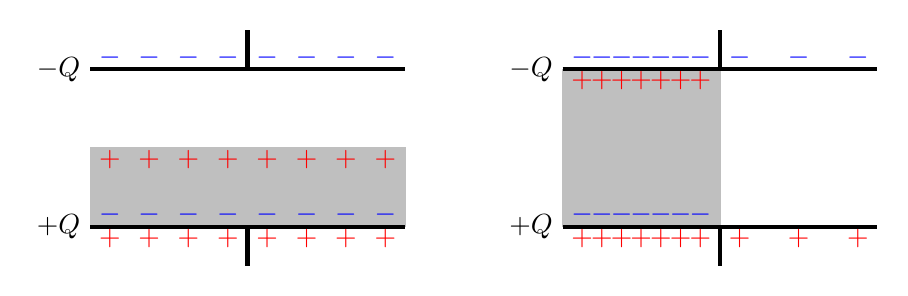
\begin{tikzpicture}
            \tikzstyle{wire} = [ultra thick]
            \tikzstyle{dielectric} = [fill=lightgray, color=lightgray]
            \tikzstyle{positive} = [color=red]
            \tikzstyle{negative} = [color=blue]
            \draw[dielectric] (0, 0) rectangle (4, 1);
            \draw[wire] (0, 0) -- (4, 0);
            \draw[wire] (0, 2) -- (4, 2);
            \draw[wire] (2, 0) -- (2, -0.5);
            \draw[wire] (2, 2) -- (2, 2.5);
            \node[left] at (0, 0) {\(+Q\)};
            \node[left] at (0, 2) {\(-Q\)};
            \foreach \x in {0.25, 0.75, ..., 3.75} {
                \node[positive] at (\x, 0.85) {\(+\)};
                \node[positive] at (\x, -0.15) {\(+\)};
                \node[negative] at (\x, 0.15) {\(-\)};
                \node[negative] at (\x, 2.15) {\(-\)};
            }
            
            \begin{scope}[xshift=6cm]
                \draw[dielectric] (0, 0) rectangle (2, 2);
                \draw[wire] (0, 0) -- (4, 0);
                \draw[wire] (0, 2) -- (4, 2);
                \draw[wire] (2, 0) -- (2, -0.5);
                \draw[wire] (2, 2) -- (2, 2.5);
                \node[left] at (0, 0) {\(+Q\)};
                \node[left] at (0, 2) {\(-Q\)};
                \foreach \x in {0.25, 0.5, ..., 1.75} {
                    \node[positive] at (\x, 1.85) {\(+\)};
                    \node[positive] at (\x, -0.15) {\(+\)};
                    \node[negative] at (\x, 0.15) {\(-\)};
                    \node[negative] at (\x, 2.15) {\(-\)};
                }
                \foreach \x in {2.25, 3, 3.75} {
                    \node[positive] at (\x, -0.15) {\(+\)};
                    \node[negative] at (\x, 2.15) {\(-\)};
                }
            \end{scope}
        \end{tikzpicture}
        \caption{The two interesting ways to half fill a capacitor with dielectric.}
        \label{fig:half filled capacitor}
    \end{figure}
    For the case of the capacitor half filled as shown on the left the addition of the dielectric does not break the planar symmetry of the situation and therefore \(\sigma_f\) is homogeneous.
    The high symmetry allows us to apply Gauss' law in media and from this we can get the displacement field and then from that we can get quantities of interest such as the electric field, polarisation field, bound charge density, potential, etc.
    For the case of the capacitor half filled as shown on the right the planar symmetry is broken and this means that Gauss' law is not as useful.
    By the symmetry of the situation we know that within the two regions, in the dielectric and outside the dielectric, the electric field is homogeneous.
    The free charge density, \(\sigma_f\), is inhomogeneous as the polarisation field distorts it.
    We therefore need to take a different approach to find the electric field we can construct equipotentials and then from the electric field we can find the displacement field and other interesting quantities.
    
    \section{The Magnetic Field in Media}
    \subsection{Types of Magnetisation}
    When an external magnetic field is applied to a material it will produce a magnetisation response.
    There are three mechanisms by which this can happen:
    \begin{itemize}
        \item Diamagnetism -- All materials have a diamagnetic response but it is only important in materials without an intrinsic magnetic moment as it is such a weak effect.
        What happens is the external magnetic field alters the angular momentum of the electrons which induces a field that opposes the external field.
        
        \item Paramagnetism -- This effect is important in materials in which each atom/molecule has an intrinsic magnetic moment and they are free to move.
        When an external field is applied these individual magnetic moments align with the field and create an induced field parallel to the applied field.
        
        \item Ferromagnetism -- This effect occurs in only a few materials.
        In these materials the intrinsic magnetic moments of individual species can align and stay aligned.
        However this is a local effect and the material will become a mosaic of `domains' where in each domain the magnetic moments of all species are aligned.
        When an external field is applied the domain boundaries will change in a way that favours domains where the magnetic moment is aligned with the external field.
        When the magnetic field is removed the domain boundaries do not return to where they where.
        This is the process by which a permanent magnet can be created.
    \end{itemize}
    
    \subsection{Magnetisation Field}
    The \define{magnetisation field}, \(\vv{M}\), is the net magnetisation dipole density in volume \(\dd{V}\):
    \[\dd{\vv{m}} = \vv{M}\dd{V}\]
    where \(\dd{\vv{m}}\) is the neg magnetic dipole moment due to the material in \(\dd{V}\).
    This is analogous to the definition of \(\vv{P}\) in section~\ref{sec:dielectric materials}.
    
    We can think of the magnetic dipole at a point as being the result of a small current loop.
    These then combine to give a macroscopic effect.
    \begin{figure}
        \centering
        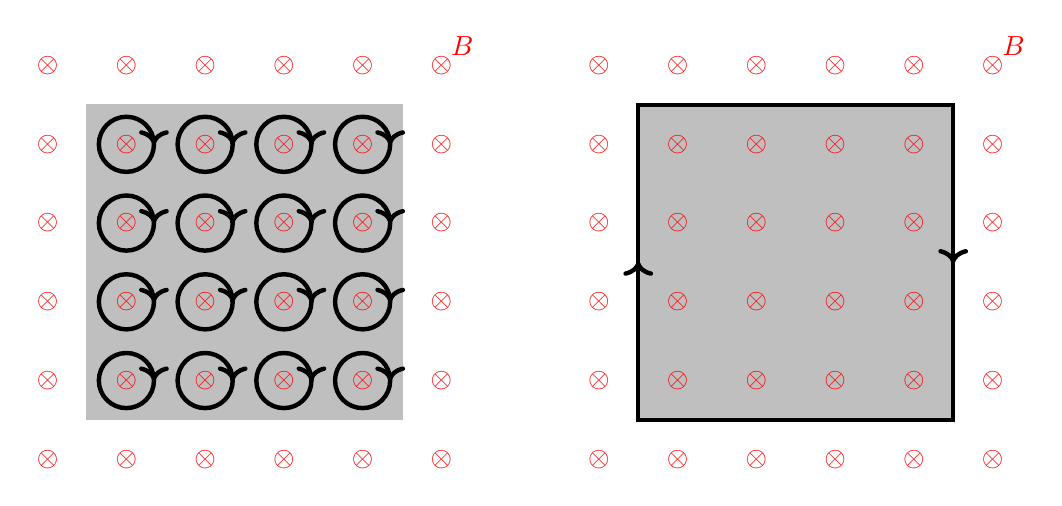
\begin{tikzpicture}
            \draw[fill=lightgray, color=lightgray] (0, 0)  rectangle (4, 4);
            \foreach \x in {0, 1, 2, 3} {
                \foreach \y in {0, 1, 2, 3} {
                    \draw[ultra thick] ($(\x, \y) + (0.5, 0.5)$) circle[radius=0.35cm];
                    \draw[ultra thick, ->] ($(\x, \y) + (0.85, 0.501)$) -- ($(\x, \y) + (0.85, 0.499)$);
                }
            }
            \foreach \x in {-0.5, 0.5, ..., 4.5} {
                \foreach \y in {-0.5, 0.5, ..., 4.5} {
                    \node[color=red] at (\x, \y) {\(\otimes\)};
                }
            }
            \node[color=red, above right] at (4.5, 4.5) {\(\vv{B}\)};
            
            \begin{scope}[xshift=1cm]
                \draw[fill=lightgray, ultra thick] (6, 0) rectangle (10, 4);
                \draw[ultra thick, ->] (10, 2.01) -- (10, 1.99);
                \draw[ultra thick, ->] (6, 1.99) -- (6, 2.01);
                \foreach \x in {5.5, 6.5, ..., 10.5} {
                    \foreach \y in {-0.5, 0.5, ..., 4.5} {
                        \node[color=red] at (\x, \y) {\(\otimes\)};
                    }
                }
                \node[color=red, above right] at (10.5, 4.5) {\(\vv{B}\)};
            \end{scope}
        \end{tikzpicture}
        \caption{Individual magnetic moments viewed as microscopic current loops vs. the net magnetic moment viewed as a macroscopic current loop.}
        \label{fig:magnetisation due to homogenous magnetic field}
    \end{figure}
    Figure~\ref{fig:magnetisation due to homogenous magnetic field} shows the net effect of many individual magnetic moments.
    In this case the magnetic field is homogenous and this results in there being no current in the material, \(\vv{J_M} = \vv{0}\).
    There is only a surface current, \(\vv{j_M}\).
    If the field were not homogenous then there would be an internal current.
    The magnetic moments for an inhomogeneous magnetic field are shown in figure~\ref{fig:magnetisation due to inhomogeneous magnetic field}
    \begin{figure}[ht]
        \centering
        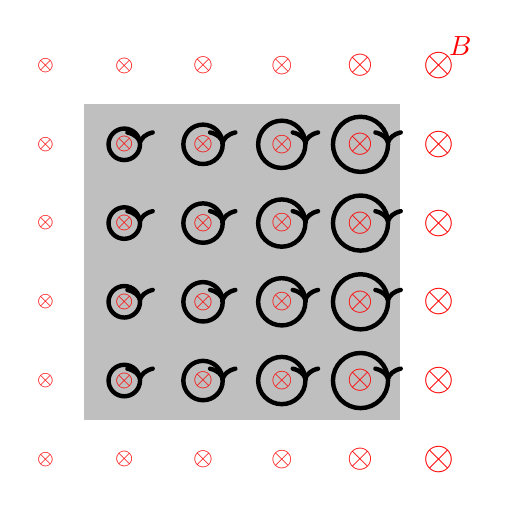
\begin{tikzpicture}
            \draw[color=lightgray, fill=lightgray] (0, 0) rectangle (4, 4);
            \foreach \y in {-0.5, 0.5, ..., 4.5} {
                \node[color=red] at (-0.5, \y) {\scriptsize \(\otimes\)};
                \node[color=red] at (0.5, \y) {\footnotesize \(\otimes\)};
                \node[color=red] at (1.5, \y) {\small \(\otimes\)};
                \node[color=red] at (2.5, \y) {\normalsize \(\otimes\)};
                \node[color=red] at (3.5, \y) {\large \(\otimes\)};
                \node[color=red] at (4.5, \y) {\Large \(\otimes\)};
            }
            \node[above right, color=red] at (4.5, 4.5) {\(\vv{B}\)};
            \foreach \y in {0.5, 1.5, ..., 3.5} {
                \draw[ultra thick] (0.5, \y) circle[radius=0.2cm];
                \draw[ultra thick, ->] ($(0.7, \y) + (0, 0.001)$) -- ($(0.7, \y) - (0, 0.001)$);
                \draw[ultra thick] (1.5, \y) circle[radius=0.25cm];
                \draw[ultra thick, ->] ($(1.75, \y) + (0, 0.001)$) -- ($(1.75, \y) - (0, 0.001)$);
                \draw[ultra thick] (2.5, \y) circle[radius=0.3cm];
                \draw[ultra thick, ->] ($(2.8, \y) + (0, 0.001)$) -- ($(2.8, \y) - (0, 0.001)$);
                \draw[ultra thick] (3.5, \y) circle[radius=0.35cm];
                \draw[ultra thick, ->] ($(3.85, \y) + (0, 0.001)$) -- ($(3.85, \y) - (0, 0.001)$);
            }
        \end{tikzpicture}
        \caption{Individual magnetic moments due to an inhomogeneous magnetic field.}
        \label{fig:magnetisation due to inhomogeneous magnetic field}
    \end{figure}
    In this case the eddy currents do not cancel and we have an internal current, \(\vv{J_M}\), as well as the surface current, \(\vv{j_M}\).
    
    We now want to quantify these effects.
    To do this we use the magnetic vector potential at \(\vv{r}\) due to an ideal magnetic dipole, \(\vv{m}\), at \(\vv{r'}\):
    \[\vv{A}(\vv{r}) = \frac{\mu_0}{4\pi} \frac{\vv{m}\times (\vv{r} - \vv{r'})}{\abs{\vv{r} - \vv{r'}}^3}.\]
    This generalises by superposition to
    \[\vv{A}(\vv{r}) = \frac{\mu_0}{4\pi} \int_V \frac{\vv{M}\times (\vv{r} - \vv{r'})}{\abs{\vv{r} - \vv{r'}}^3}\dd[3]{r'}.\]
    We then use the identity
    \[\frac{\vv{r} - \vv{r'}}{\abs{\vv{r} - \vv{r'}}^3} = \grad' \frac{1}{\abs{\vv{r} - \vv{r'}}}\]
    where \(\grad'\) is the gradient operator that acts only on \(\vv{r'}\).
    Hence
    \[\vv{A}(\vv{r}) = \frac{\mu_0}{4\pi} \int_V \vv{M}(\vv{r'}) \times \grad'\left[\frac{1}{\abs{\vv{r} - \vv{r'}}}\right] \dd[3]{r'}.\]
    We then use the product rule, \(\curl(f\vv{K}) = f\curl\vv{K} - \vv{K}\times\grad f\), to get
    \begin{align*}
        \vv{A}(\vv{r}) &= \frac{\mu_0}{4\pi} \int_V \frac{\grad'\times\vv{M}(\vv{r'})}{\abs{\vv{r} - \vv{r'}}} \dd[3]{r'} - \frac{\mu_0}{4\pi} \int_V \curl\left[\frac{\vv{M}(\vv{r'})}{\abs{\vv{r} - \vv{r'}}}\right] \dd[3]{r'}\\
        &= \frac{\mu_0}{4\pi} \int_V \frac{\grad'\times\vv{M}(\vv{r'})}{\abs{\vv{r} - \vv{r'}}} \dd[3]{r'} - \frac{\mu_0}{5\pi} \oint_S \left[\frac{\vv{M(\vv{r'})}}{\abs{\vv{r} - \vv{r'}}}\right]\times \dd{\vv{S'}}.
    \end{align*}
    Recall that
    \[\laplacian\vv{A} = \mu_0\vv{J} \implies \vv{A} = \frac{\mu_0}{4\pi} \int_V \frac{\vv{J}(\vv{r'})}{\abs{\vv{r} - \vv{r'}}}\dd[3]{r'}.\]
    This allows us to interpret the numerators of both integrands as currents.
    First
    \[\vv{J_M} = \curl\vv{M}\]
    is the bulk magnetisation current density, second
    \[\vv{j_M} = \vv{M}\times\vh{n}\]
    is the surface current density where \(\vh{n}\) is normal to the surface \(S'\) which bounds the volume \(V'\).
    
    \begin{example}
        A cylindrical bar magnet has uniform magnetisation, \(M\), along its axis.
        To what current distribution is this equivalent?
        
        \(\vv{M}\) is uniform so \(\curl\vv{M} = \vv{0}\) meaning \(\vv{J_M} = 0\).
        The surface current density is then
        \[\vv{j_M} = \vv{M}\times\vh{n} = M\ve{z}\times\ve{\rho} = M\ve{\varphi}.\]
        This has magnitude \(M\) and is `solenoidal', i.e. it resembles a solenoid with current flow around the circumference of a cylinder.
    \end{example}
    \begin{example}
        A long cylindrical bar magnet of uniform magnetisation is bent into a loop.
        To what current distribution is this equivalent?
        
        The curl in cylindrical coordinates is
        \[\curl\vv{M} = \left[\frac{1}{\rho}\pdv{M_z}{\varphi} - \pdv{M_\varphi}{z}\right]\ve{\rho} + \left[\pdv{M_\rho}{z} - \pdv{M_z}{\rho}\right]\ve{\varphi} + \frac{1}{\rho}\left[\pdv{\rho}(\rho M_\varphi) - \pdv{M_\rho}{\varphi}\right]\ve{z}.\]
        With this setup \(\vv{M}\) is circumferential so \(\vv{M} = M\ve{\varphi}\) so \(M_\rho = M_z = 0\) meaning that the curl reduces to
        \[\curl\vv{M} = \frac{1}{\rho}\pdv{\rho}(\rho M) = \frac{M}{\rho}\ve{z} = \vv{J_M}.\]
        The surface current has magnitude \(M\) and wraps around the cylinder still.
        The surface current is `toroidal', i.e. it resembles a toroidal solenoid with current flow over the surface.
        The bulk current density makes up for the fact that due to the geometry the net surface current is greater on the outside of the torus than the inside due to the greater surface area.
    \end{example}
    
    \subsection{Amp\`ere's Law in Media}
    The Amp\`ere--Maxwell law in a vacuum is
    \[\curl\vv{B} = \mu_0(\vv{J} + \varepsilon\partial_t\vv{E}).\]
    We divide \(\vv{J}\) into three parts: \(\vv{J_f}\) which is the current due to free charges, this is the normal current with which we have dealt so far, \(\vv{J_M} = \curl\vv{M}\) which is the magnetisation current as defined in the previous section, and \(\vv{J_P}\) which is the polarisation current which accounts for the movement of electric dipoles.
    To rationalise the introduction of \(\vv{J_P}\) we define a new charge density, \(\rho_P = -\div\vv{P}\), which follows the continuity equation
    \[\partial_t \rho_P + \div\vv{J_P} = 0.\]
    From this we have
    \[\vv{J_P} = \partial_t\vv{P}.\]
    We aim to write the Amp\`ere--Maxwell law in terms of \(\vv{J_f}\) only:
    \begin{align*}
        \curl\vv{B} &= \mu_0 (\vv{J_f} + \vv{J_M} + \vv{J_P} + \varepsilon_0\partial_t\vv{E})\\
        &= \mu_0(\vv{J_f} + \curl\vv{M} + \partial_t\vv{P} + \varepsilon_0\partial_t\vv{E})\\
        &= \mu_0(\vv{J_f} + \curl\vv{M} + \partial_t\vv{D})
    \end{align*}
    From this we have
    \[\curl\left[\frac{1}{\mu_0}\vv{B} - \vv{M}\right] = \vv{J_f} + \partial_t\vv{D}.\]
    We then define
    \[\vv{H} = \frac{1}{\mu_0}\vv{B} - \vv{M}\]
    so
    \[\curl\vv{H} = \vv{J_f} + \partial_t\vv{D}.\]
    This is the Amp\`ere--Maxwell law in media.
    In integral form it reads
    \[\oint_C \vv{H}\cdot\dd{\vv{l}} = \int_S (\vv{J_f} + \partial_t\vv{D})\cdot\dd{\vv{S}} = I_{f, \enc},\]
    where \(C\) is the contour bounding the surface \(S\).
    
    Confusingly \(\vv{H}\) is often referred to as the `magnetic field' and so is \(\vv{B}\).
    In some texts \(\vv{B}\) is the `magnetic flux density' and \(\vv{H}\) is the `magnetic field strength' but in other texts \(\vv{B}\) is the `magnetic field' and \(\vv{H}\) is the `auxiliary field'.
    For this reason it is best to specify `the magnetic \(\vv{B}\) field' or `the magnetic \(\vv{H}\) field'.
    
    Maxwell's second and third laws do not need modification in media as they contain no source terms, \(\rho\) or \(\vv{J}\).
    This means that we now have the four Maxwell equations in media:
    \begin{align*}
        \div\vv{D} &= \rho_f \tag{MI in media}\\
        \div\vv{B} &= 0 \tag{MII}\\
        \curl\vv{E} &= -\partial_t\vv{B} \tag{MIII}\\
        \curl\vv{H} &= \vv{J_f} + \partial_t\vv{D} \tag{MIV in media}
    \end{align*}
    
    We define the \define{magnetic susceptibility}, \(\chi_M\), to describe the relationship between \(\vv{M}\) and \(\vv{H}\):\footnote{some texts use \(\chi_B\vv{B} = \mu_0\vv{M}\) instead, these are related by \(\chi_B = \chi_M/(1 + \chi_M)\)}
    \[\vv{M} = \chi_M\vv{H}.\]
    In general \(\chi_M\) is a tensor however in \gls{lih} media it is a scalar.
    From this we also have
    \[\vv{B} = \mu_r\mu_0\vv{H} = \mu_0(1 + \chi_M)\vv{H} = \mu\vv{H}\]
    where \(\mu_r = 1 + \chi_M\) is the \define{relative permeability} and \(\mu = \mu_0\mu_r\) is the \define{absolute permeability}.
    In the absence of magnetisation \(\chi_M = 0\) and \(\mu_r = 1\).
    Unlike with dielectrics \(\chi_M\) can be positive or negative and consequently \(\mu_r\) is unbounded.
    For example a diamagnetic material will have \(\chi_M < 0\) whereas a paramagnetic material will have \(\chi_M > 0\) which corresponds to the fact that the fields induced in these two materials will be in opposite directions.
    
    \subsection{Media in Solenoids}
    A solenoid is filled with \gls{lih} medium with magnetic susceptibility \(\chi_M\).
    What is the effect compared to a solenoid containing a vacuum?
    
    The magnetisation field is given by \(\vv{M} = \chi_M\vv{H}\).
    The inductance of a solenoid is given by \(L = \Phi_B/I\).
    We first get \(\vv{H}\) from
    \[\curl\vv{H} = \vv{J_f} + \partial_t\vv{D} \implies \oint_C \vv{H}\cdot\dd{\vv{l}} = I_{f, \enc}.\]
    By symmetry we know that \(\vv{H}\) is axial and constant inside the solenoid and zero outside the solenoid.
    Thus if we define an Amp\'erian loop we only need integrate along the part inside the solenoid parallel to the axis.
    If this part has length \(l\) then
    \[\oint_C\vv{H}\cdot\dd{\vv{l}} = Hl = I_{f, \enc} = nlI \implies H_z = nI\]
    where \(n\) is the number of loops the solenoid has per unit length.
    From this we have
    \[\vv{B} = \mu_0\mu_r\vv{H} = \mu_0(1 + \chi_M)hI\ve{z}.\]
    This allows us to calculate the flux through the inductor treating the inductor as \(n\) loops of area \(A\) per unit length we have
    \[\Phi_B = ABnl = \mu_0(1 + \chi_M)n^2AlI\]
    where \(A\) is the cross sectional area of the solenoid.
    So the inductance is
    \[L = \frac{\Phi_B}{I} = \mu_0(1 + \chi_M)n^2Al = \mu_0(1 + \chi_M)n^2V_s\]
    where \(V_s = Al\) is the volume of the solenoid.
    
    \subsubsection{Partially Filled Solenoids}
    There are two interesting ways to half fill a solenoid.
    The first is with a cylindrical core which has a radius smaller than the solenoid.
    This preserves the cylindrical symmetry and therefore we can use Amp\`ere's law with two different cases, one that reaches all the way to the media and the other which stops in the vacuum.
    
    The second is with a cylindrical core that is of the same radius as the solenoid but doesn't extend for the solenoids entire length.
    This breaks the cylindrical symmetry.
    We can view this as two contributions, one from the filled section and one from the empty section.
    We cannot use Amp\`ere's law in this scenario to find the field.
    
    \section{Electromagnetism in Media}
    \subsection{Summary}
    Maxwell's equations for the macroscopic fields, \(\vv{D}\), \(\vv{B}\), \(\vv{E}\), and \(\vv{H}\), in media with free charge density, \(\rho_f\), and free current density, \(\vv{J_f}\), are
    \begin{align*}
        \div\vv{D} &= \rho_f, \tag{MI in media}\\ 
        \div\vv{B} &= 0, \tag{MII}\\
        \curl\vv{E} &= -\partial_t\vv{B},\tag{MIII}\\
        \curl\vv{H} &= \vv{J_f} + \partial_t\vv{D},\tag{MIV in media}
    \end{align*}
    Where the fields, \(\vv{D}\) and \(\vv{H}\), are defined as
    \[\vv{D} = \varepsilon_0\vv{E} + \vv{P},\qquad\text{and}\qquad \vv{B} = \mu_0(\vv{H} + \vv{M}).\]
    The free charges and currents satisfy the continuity equation
    \[\partial_t\rho_f + \div\vv{J_f} = 0.\]
    In \gls{lih} media the relations between the fields are
    \[\vv{P} = \chi_E\varepsilon_0\vv{E}, \qquad \vv{M} = \chi_M\vv{H}, \qquad \vv{D} = \varepsilon_0\varepsilon_r\vv{E} = \varepsilon\vv{E},\]
    \[\text{and}\qquad \vv{B} = \mu_0\mu_r\vv{H} = \mu\vv{H}.\]
    Where \(\varepsilon_r = 1 + \chi_E\) and \(\mu_r = 1 + \chi_M\).
    
    \subsection{Energy Density and the Poynting Vector}
    The power delivered by an \gls{em} field to a system of charge carriers is \(\vv{E}\cdot\vv{J_f}\) per unit volume.
    This means that the energy density, \(u\), obeys
    \[\dv{u}{t} = \vv{E}\cdot\vv{J_f}.\]
    We aim to express \(\vv{J_f}\) in field related quantities.
    First we use Maxwell's fourth law to write
    \[\vv{E}\cdot\vv{J_f} = \vv{E}\cdot\left[\curl\vv{H} - \partial_t\vv{D}\right] = \vv{E}\cdot(\curl\vv{H}) - \vv{E}\cdot\partial_t\vv{D}.\]
    We then use the product rule,
    \[\div(\vv{E}\times\vv{H}) = \vv{H}\cdot(\curl\vv{E}) - \vv{E}\cdot(\curl\vv{H}) \implies \vv{E}\cdot(\curl\vv{H}) - \vv{E}\cdot(\curl\vv{H}) - \div(\vv{E}\times\vv{H}),\]
    to get
    \[\vv{E}\cdot\vv{J} = \vv{H}\cdot(\curl\vv{E}) - \div(\vv{E}\times\vv{H}) - \vv{E}\cdot\partial_t\vv{D}.\]
    Using Maxwell's third law this becomes
    \[\vv{E}\cdot\vv{J_f} = -\vv{H}\cdot\partial_t\vv{B} - \div(\vv{E}\times\vv{H}) - \vv{E}\cdot\partial_t\vv{D}.\]
    Next we use that in \gls{lih} media
    \[\vv{E}\cdot\partial_t\vv{D} = \vv{E}\cdot\partial_t(\varepsilon\vv{E}) = \varepsilon\vv{E}\cdot\partial_t\vv{E} = \vv{D}\cdot\partial_t\vv{E}\]
    and
    \[\vv{H}\cdot\partial_t\vv{B} = \mu\vv{B}\cdot\partial_t\vv{B} = \vv{B}\cdot\partial_t(\mu\vv{B}) = \vv{B}\cdot\partial_t\vv{H}.\]
    This gives us
    \[\vv{E}\cdot\vv{J_f} = -\vv{B}\cdot\partial_t\vv{H} - \vv{D}\cdot\partial_t\vv{E} - \div(\vv{E}\times\vv{H}).\]
    Recognising the standard product rule
    \[\partial_t(\vv{E} \cdot \vv{D}) = \vv{D}\cdot\partial_t\vv{E} + \vv{E}\cdot\partial_t\vv{D} = 2\vv{D}\cdot\partial_t\vv{E}\]
    and similarly for the magnetic fields this becomes
    \[\vv{E}\cdot\vv{J_f} = \frac{1}{2}\partial_t(\vv{E}\cdot\vv{D} + \vv{B}\cdot\vv{H}).\]
    We then integrate over a volume, \(V\), to get the energy from the energy density.
    Using the divergence theorem on the second term we get
    \[\dv{U}{t} = -\frac{1}{2}\dv{t}\int_V (\vv{E}\cdot\vv{D} + \vv{B}\cdot\vv{H})\dd{V} - \oint_A(\vv{E}\times\vv{H})\cdot\dd{\vv{A}}.\]
    We now identify the electric and magnetic energy densities as
    \[u_E = \frac{1}{2}\vv{E}\cdot\vv{D}, \qquad\text{and}\qquad u_M = \frac{1}{2}\vv{B}\cdot\vv{H}\]
    respectively.
    From the second term we identify the macroscopic Poynting vector as
    \[\vv{S} = \vv{E}\times\vv{H}\]
    so the power delivered to the charges can be written as
    \[\dv{U}{t} = -\dv{t}[U_E + U_M] - \oint_A\vv{S}\cdot\dd{\vv{A}}.\]
    
    \subsection{Boundary Conditions}
    \subsubsection{Qualitatively}
    Now that we have characterised fields in and out of media we want to know how the fields behave at the boundary between media.
    To do this we use the work we have done already with half filled capacitors/inductors and we make the unjustified assumption that the same analysis holds outside of a capacitor/inductor.
    Figure~\ref{fig:fields at boundaries} shows qualitatively what happens at a boundary for the four fields, this figure assumes that \(\chi_M > 0\).
    The two cases we consider for each field are what happens to the tangential component and the normal component at the boundary.
    \begin{figure}[ht]
        \centering
        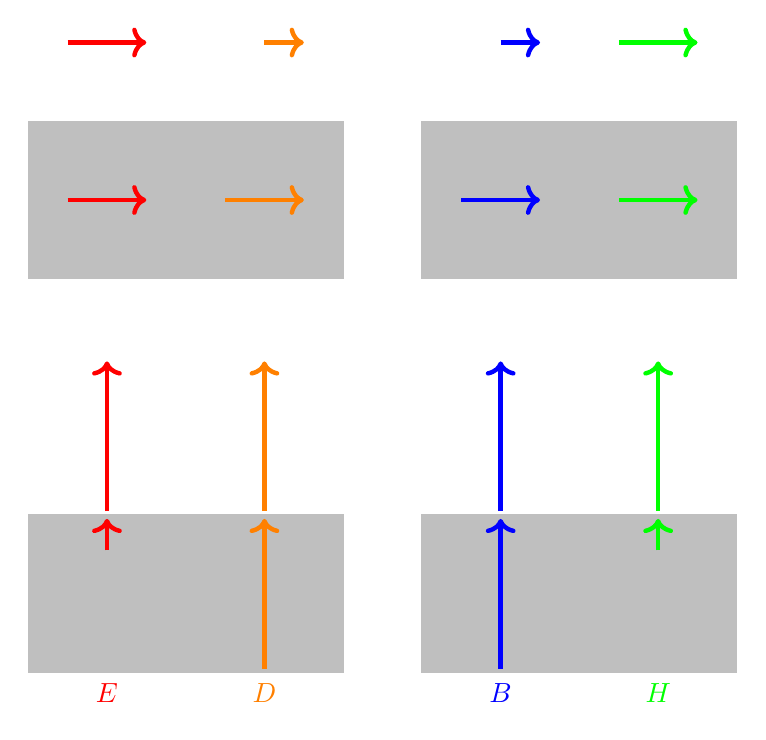
\begin{tikzpicture}
            \tikzstyle{media} = [fill=lightgray, color=lightgray]
            \tikzstyle{field} = [ultra thick, ->]
            \tikzstyle{E} = [field, color=red]
            \tikzstyle{B} = [field, color=blue]
            \tikzstyle{D} = [field, color=orange]
            \tikzstyle{H} = [field, color=green]
            \draw[media] (0, 0) rectangle (4, 2);
            \draw[media] (5, 0) rectangle (9, 2);
            \draw[media] (0, 5) rectangle (4, 7);
            \draw[media] (5, 5) rectangle (9, 7);
            \draw[E] (1, 1.55) -- (1, 1.95);
            \draw[E] (1, 2.05) -- (1, 3.95);
            \draw[D] (3, 0.05) -- (3, 1.95);
            \draw[D] (3, 2.05) -- (3, 3.95);
            \draw[E] (0.5, 6) -- (1.5, 6);
            \draw[E] (0.5, 8) -- (1.5, 8);
            \draw[D] (2.5, 6) -- (3.5, 6);
            \draw[D] (3, 8) -- (3.5, 8);
            \draw[B] (6, 0.05) -- (6, 1.95);
            \draw[B] (6, 2.05) -- (6, 3.95);
            \draw[H] (8, 1.55) -- (8, 1.95);
            \draw[H] (8, 2.05) -- (8, 3.95);
            \draw[B] (5.5, 6) -- (6.5, 6);
            \draw[B] (6, 8) -- (6.5, 8);
            \draw[H] (7.5, 6) -- (8.5, 6);
            \draw[H] (7.5, 8) -- (8.5, 8);
            
            \node[below, E] at (1, 0) {\(\vv{E}\)};
            \node[below, D] at (3, 0) {\(\vv{D}\)};
            \node[below, B] at (6, 0) {\(\vv{B}\)};
            \node[below, H] at (8, 0) {\(\vv{H}\)};
        \end{tikzpicture}
        \caption{The qualitative behaviour of fields at a boundary between media. The normal and tangential components of the four fields are shown both in the media and outside.}
        \label{fig:fields at boundaries}
    \end{figure}
    \subsubsection{Quantitatively}
    We can be much more rigorous if we use Maxwell's laws.
    We assume we have a plane and above and below the plane are two different media, media 1 below and media 2 above.
    We use a Gaussian surface that is a cylindrical pill box of height \(h\) with the flat faces parallel to the plane, and a rectangular Amp\'erian loop of height \(h\) with two sides running parallel to the plane.
    We also define two vectors, \(\vh{n}\), and \(\vh{t}\), which are normal and tangential to the plane respectively.
    
    The first condition we consider is Maxwell's first law,
    \[\div\vv{D} = \rho_f.\]
    From this and the divergence theorem we have
    \[\oint_S\vv{D}\cdot\dd{\vv{S}} = Q_{f, \enc}.\]
    pill box has a surface normal, on the flat faces, of \(\dd{\vv{S}} = \vh{n}\dd{S}\).
    Allowing \(h\to 0\) we can ignore the contribution to the integral from the sides of the pill box and we get
    \[\int\vv{D}\cdot\dd{\vv{S}} = \int(\vv{D_2} - \vv{D_1})\cdot\vh{n}\dd{S} = \int \sigma_f \dd{S}\]
    where the last equality arises from the definition of a surface charge density.
    Note that \(\vv{D_1}\) is the \(\vv{D}\) field below the plane and \(\vv{D_2}\) is the \(\vv{D}\) field above the plane.
    Since both integrals are over the same area we can conclude that
    \[(\vv{D_2} - \vv{D_1})\cdot\vh{n} = \sigma_f.\]
    Taking the scalar product with \(\vh{n}\) picks out the scalar component of \(\vv{D_2} - \vv{D_1}\) and so \(\vv{D_{\mathrm{normal}}}\) is continuous \emph{if and only if} \(\sigma_f = 0\).
    
    The second condition we consider is Maxwell's second law,
    \[\div\vv{B} = 0 \implies \oint_S \vv{B}\cdot\dd{\vv{S}} = 0.\]
    Using the same Gaussian surface and again allowing \(h\to 0\) we have
    \[\int\vv{B}\cdot\dd{\vv{S}} = \int (\vv{B_2} - \vv{B_1})\cdot\vh{n}\dd{S} = 0.\]
    This holds for any similarly defined surface so
    \[(\vv{B_2} - \vv{B_1})\cdot\vh{n} = 0\]
    meaning that \(\vv{B_{\mathrm{normal}}}\) is \emph{always} continuous.
    
    The third condition we consider is Maxwell's third law,
    \[\curl\vv{E} = -\partial_t\vv{B} \implies \oint_C\vv{E}\cdot\dd{\vv{l}} = -\partial_t\Phi_B.\]
    We use an Amp\'erian loop of length \(\ell\) and height \(h\).
    Allowing \(h\to -\) we also have \(\Phi_B\to 0\) as long as \(B\) is finite.
    Therefore
    \[\int \vv{E}\cdot\dd{\vv{l}} = \int(\vv{E_2} - \vv{E_1})\cdot\vh{t} \dd{l} = 0\]
    where \(\vh{t}\) is tangential to the surface meaning that \(\vh{t}\cdot\vh{n} = 0\).
    Since this holds no matter where we put the Amp\'erian loop, or define \(\vh{t}\) we have
    \[(\vv{E_2} - \vv{E_1})\cdot\vh{t} = 0\]
    meaning that \(\vv{E_{\mathrm{tangential}}}\) is \emph{always} continuous.
    
    The final condition that we consider is Maxwell's fourth law
    \[\curl\vv{H} = \vv{J_f} + \partial_t\vv{D}\]
    in integral form this becomes
    \[\oint_{C}\vv{H}\cdot\dd{\vv{l}} = \vv{j_f} \cdot \vh{s}\ell + (\partial_t\vv{D})\cdot\vh{s}\ell h\]
    where \(\vv{j_f}\) is the free surface current per unit area and \(\vh{s} = \vh{t}\times\vh{n}\) is the surface unit vector perpendicular to the Amp\'erian loop.
    Now allowing \(h\to 0\) we have
    \[\int\vv{H}\cdot\dd{\vv{l}} = \vv{H_1} - \vv{H_2})\cdot\vh{t}\ell = \vh{j_f}\cdot\vh{s}\ell.\]
    Since \(\vh{n}\) is normal to the plane \(\vh{s}\) is tangential to the plane so \(\vv{H_\mathrm{tangential}}\) is continuous \emph{if and only if} \(\vv{j_f} = \vv{0}\).
    This general form can be written in other ways, including
    \begin{align*}
        (\vv{H_1} - \vv{H_2})\cdot\vh{t} &= \vv{j_f}\cdot\vh{s},\\
        (\vv{H_{2, \mathrm{tangential}}} - \vv{H_{1, \mathrm{tangential}}}) &= \vv{j_f}\times\vh{n},\\
        (\vv{H_2} - \vv{H_1})\times\vh{n} &= -\vv{j_f}.
    \end{align*}

    In summary at a boundary between media
    \begin{itemize}
        \item \(\vv{D_{\mathrm{normal}}}\) is continuous if and only if \(\sigma_f = 0\).
        \item \(\vv{B_{\mathrm{normal}}}\) is continuous always.
        \item \(\vv{E_{\mathrm{tangential}}}\) is continuous always.
        \item \(\vv{H_{\mathrm{tangential}}}\) is continuous if and only if \(\vv{j_f} = \vv{0}\).
    \end{itemize}

    \section{Continuity Conditions and Waves in Media}
    \subsection{Applications of Continuity Conditions}
    \subsubsection{Inclined Dielectric}
    Consider the setup in figure~\ref{fig:refraction}.
    \begin{figure}[ht]
        \centering
        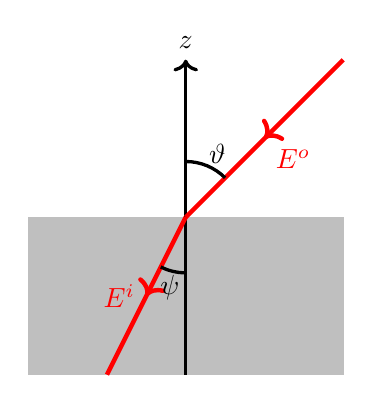
\begin{tikzpicture}
            \tikzstyle{mid arrow} = [postaction={decorate, decoration={markings, mark=at position .5 with {\arrow{>}}}}]
            \tikzstyle{E base} = [ultra thick, color=red]
            \tikzstyle{E} = [E base, mid arrow]
            \tikzstyle{angle} = [very thick]
            \tikzstyle{media} = [color=lightgray, fill=lightgray]
            \tikzstyle{axis} = [very thick, ->]
            \draw[media] (-2, -2) rectangle (2, 0);
            \draw[axis] (0, -2) -- (0, 2) node[above] {\(z\)};
            \draw[E] (2, 2) -- (0, 0);
            \draw[E] (0, 0) -- (-1, -2);
            \draw[angle] (0.5, 0.5) arc[start angle=45, end angle=90, radius=0.707cm];
            \draw[angle] (0, -0.707) arc[start angle=-90, end angle=-116.6, radius=0.707cm];
            \node[below right, E base] at (1, 1) {\(\vv{E^o}\)};
            \node[left, E base] at (-0.5, -1) {\(\vv{E^i}\)};
            \node at (0.4, 0.8) {\(\vartheta\)};
            \node at (-0.2, -0.9) {\(\psi\)};
        \end{tikzpicture}
        \caption{An inclined dielectric with an incident electric field.}
        \label{fig:refraction}
    \end{figure}
    It shows a uniform electric field, \(\vv{E^o}\), incident on a dielectric at an angle \(\vartheta\).
    The field is then refracted and the field in the dielectric is at an angle \(\psi\).
    We want to know what the field, \(\vv{E^i}\), inside the dielectric is.
    
    Outside the dielectric we define the displacement field as
    \[\vv{D^o} = \varepsilon_0\vv{E^o}.\]
    Inside the dielectric the displacement field is
    \[\vv{D^i} = \varepsilon_0\varepsilon_r\vv{E^i}.\]
    We apply the boundary condition that the normal component of the displacement field, \(D_n\), is continuous at the boundary, since there is no surface charge.
    This means that \(D^o_z = D^i_z\).
    The second boundary condition is that the tangential components of the electric field, \(E_t\), are continuous at the boundary.
    This means that \(E^o_x = E^i_x\) and \(E^o_y = E^i_y\).
    We choose a coordinate system such that \(E^o_y = E^i_y = 0\) meaning that we can work in the two-dimensional \((x, z)\)-plane.
    In this plane the full fields are
    \[\vv{E^o} = (E^o\sin\vartheta, E^o\cos\vartheta), \qquad\text{and}\qquad \vv{E^i} = (E^i\sin\psi, E^i\cos\psi).\]
    Applying the first continuity condition we have
    \[D^o_z = D_i^z \implies \varepsilon_0E^o\cos\vartheta = \varepsilon_0\varepsilon_rE^i\cos\psi \implies E^i = \frac{1}{\varepsilon_r}E^o\frac{\cos\vartheta}{\cos\psi}.\]
    Applying the second continuity condition we have
    \[E^o_x = E^i_x \implies E^o\sin\vartheta = E^i\sin\psi \implies E^i = E^o\frac{\sin\vartheta}{\sin\psi}.\]
    Combining these we have
    \[\frac{1}{\varepsilon_r}\frac{\cos\vartheta}{\cos\psi} = \frac{\sin\vartheta}{\sin\psi} \implies \frac{\sin\psi}{\cos\psi} = \tan\psi = \varepsilon_r\frac{\sin\vartheta}{\cos\vartheta} = \varepsilon_r\tan\vartheta \implies \psi = \arctan(\varepsilon_r\tan\vartheta).\]
    It is worth checking two basic case here.
    First we consider the case when \(\vartheta = 0\).
    In this case \(\psi = \arctan(\varepsilon_r\tan 0) = \arctan 0 = 0\) and so there is no refraction which is what we would expect.
    Going a step further back in the calculation if \(\psi = \vartheta = 0\) then we recover that \(D^o_z = D^i_z\).
    The second case we consider is \(\vartheta = \pi/2\).
    In this case \(\psi = \arctan(\varepsilon_r\tan(\pi/2)) = \arctan(\infty) = \pi/2\) and so there is no refraction as the field travels along the boundary.
    Going a step further back in the calculation if \(\psi = \vartheta = \pi/2 \) then we recover \(E^o = E^i\).
    
    \subsubsection{Spherical Cavity in a Dielectric}
    Suppose we have a large block of \gls{lih} dielectric which contains a spherical cavity.
    The electric field far from the cavity is uniform and has magnitude \(E_0\).
    What are \(\vv{E}\) and \(\vv{D}\) in the cavity?
    
    We will use spherical coordinates with their origin at the centre of the cavity and aligned so that the \(z\)-axis is parallel to the field at large \(r\).
    See figure~\ref{fig:spherical cavity} for a diagram.
    \begin{figure}[ht]
        \centering
        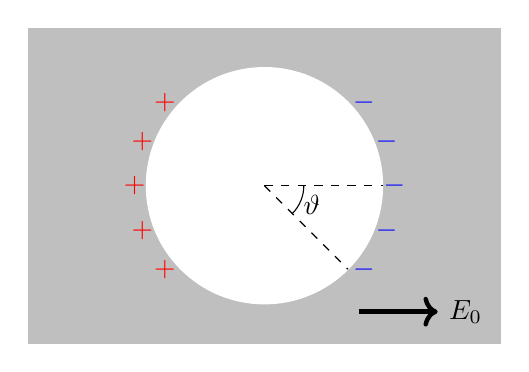
\begin{tikzpicture}
            \tikzstyle{media} = [color=lightgray, fill=lightgray]
            \tikzstyle{E} = [->, ultra thick]
            \draw[media] (-3, -2) rectangle (3, 2);
            \draw[fill=white, color=white] (0, 0) circle[radius=1.5cm];
            \draw[dashed] (0, 0) -- (1.5, 0);
            \draw[dashed] (0, 0) -- (1.06, -1.06);
            \draw (0.5, 0) arc[start angle=0, end angle=-45, radius=0.5cm];
            \node at (-22.5:0.65) {\(\vartheta\)};
            \foreach \x in {0, -20, 20, 40, -40} {
                \node[color=red] at ($({-1*cos(\x)*1.65}, {sin(\x)*1.65})$) {\(+\)};
                \node[color=blue] at ($({cos(\x)*1.65}, {sin(\x)*1.65})$) {\(-\)};
            }
            \draw[E] (1.2, -1.6) -- (2.2, -1.6) node[right] {\(\vv{E_0}\)};
        \end{tikzpicture}
        \caption{A spherical cavity in a dielectric}
        \label{fig:spherical cavity}
    \end{figure}
    At the surface of the cavity a charge distribution, \(\sigma_P = \vv{P}\cdot\vh{n}\) forms.
    Note that \(\vh{n}\) is the outward normal of the dielectric, meaning it points \emph{towards} the origin.
    Since this is an \gls{lih} media \(\vv{P}\) is parallel to \(\vv{E}\) and so the field inside is enhanced by the charge distribution which is a function of the angle, \(\vartheta\), since \(r = 1.5\) on the surface of the cavity and the symmetry under changing \(\varphi\) means that \(\sigma_P\) cannot depend on \(\varphi\).
    
    The charge distribution, \(\sigma_P(\vartheta)\), forms an effective dipole.
    Outside of the cavity the field lines are locally distorted by this charge distribution.
    We want to determine \(V\), the electrostatic potential, and from this we can calculate \(\vv{E}\).
    Within the cavity we assume a uniform \(\vv{E}\) field in the \(z\) direction.
    This corresponds to a potential
    \[V(r) = -E_{\text{in}}z = -E_{\text{in}}r\cos\vartheta\]
    for \(r < a\) where \(a\) is the radius of the cavity.
    Outside of the cavity we use a superposition of a uniform \(\vv{E_0}\) field plus a dipole field so
    \[V(r) = -E_0r\cos\vartheta + \frac{A\cos\vartheta}{r^2}.\]
    Here \(A\) is a constant to be found which gives the relative strength of the dipole field.
    
    Thanks to the uniqueness theorem for Poisson's equation we need only show that this potential fulfils the boundary conditions and Poisson's equation and then we know that the electric field derived from this potential is unique.
    Since the charges are only on the boundary away from the boundary we only need the potential to satisfy Laplace's equation, \(\laplacian V = 0\).
    We then only need to check that the boundary conditions are satisfied.
    In spherical coordinates
    \[\grad V = \ve{r}\pdv{V}{r} + \ve{\vartheta}\frac{1}{r}\pdv{V}{\vartheta} + \ve{\varphi}\frac{1}{r\sin\vartheta}\pdv{V}{\vartheta} = -\vv{E}.\]
    The first boundary condition we check is that \(E_t\) is continuous.
    This requires \(E_\vartheta\) to be continuous at \(r = a\).
    So
    \[-E_0a\sin\vartheta + \frac{A\sin\vartheta}{a^2} = -E_{\text{in}}a\sin\vartheta.\]
    The second boundary condition is that \(D_n\) is continuous (note the surface density is due to polarisation, there is no free charge distribution).
    This requires \(D_r = \varepsilon_rE_r = -\varepsilon_r\partial_rV\) to be continuous.
    So
    \[\varepsilon_rE_o\cos\vartheta + \frac{2A\varepsilon_r\cos\vartheta}{a^3} = E_{\text{in}}\cos\vartheta.\]
    Combining these we have
    \[E_{\text{in}} = \varepsilon_r\left(E_0 + \frac{2A}{a^3}\right) = E_0 - \frac{A}{a^3}.\]
    Thus
    \[E_{\text{in}} = E_0\frac{3\varepsilon_r}{1 + 2\varepsilon_r}.\]
    Combining this with the requirement that \(\vv{E_{\mathrm{in}}} = E_{\mathrm{in}}\ve{z}\) and \(\vv{D_{\mathrm{in}}} = \varepsilon_0\vv{E_{\mathrm{in}}}\) (since inside the cavity \(\varepsilon_r = 1\)), we have the full field.
    Notice that \(E_{\text{in}} > E_0\) so the field in the cavity is stronger than the field outside.
    
    \subsection{Waves in Media}
    \subsubsection{Non-conduction Media}
    In a non-conducting media \(\rho_f = 0\) and \(\vv{J_f} = 0\).
    Thus
    \[\vv{D} = \varepsilon\vv{E}, \qquad\text{and}\qquad \vv{B} = \mu\vv{H}.\]
    We can derive macroscopic wave equations as before:
    \[\laplacian\vv{E} = \varepsilon\mu \pdv[2]{\vv{E}}{t}, \qquad\text{and}\qquad \laplacian\vv{B} = \varepsilon\mu\pdv[2]{\vv{B}}{t}.\]
    Clearly these have the normal plane wave solutions
    \[\vv{E} = \vv{E_0}e^{i(\vv{k}\cdot\vv{r} - \omega t)}, \qquad\text{and}\qquad \vv{B} = \vv{B_0}e^{i(\vv{k}\cdot\vv{r} - \omega t)}.\]
    Where \(k^2 = \mu\varepsilon\omega^2\).
    We interpret this as the wave phase velocity being
    \[v = \frac{\omega}{k} = \frac{1}{\sqrt{\mu\varepsilon}}.\]
    Recall that \(c = (\mu_0\varepsilon_0)^{-1/2}\) so
    \[v^2 = \frac{1}{\mu_r\varepsilon_r}c^2 = \frac{1}{n^2}c^2\]
    where we have defined \(n = \mu_r\varepsilon_r\) which is called the \define{refractive index} and is a property of the medium.
    As we did with waves in a vacuum it can be shown that
    \[i\vv{k}\cdot\vv{E_0} = 0, \qquad\text{and}\qquad i\vv{k}\cdot\vv{B_0} = 0.\]
    This means that \(\vv{E}\) and \(\vv{B}\) are perpendicular to the direction of propagation, \(\vv{k}\), and therefore the wave is transverse.
    We see that for \gls{lih} media all of the extra complications that come with having media are neatly hidden away in \(\varepsilon\) and \(\mu\) and have the net effect of changing the velocity of the wave.
    
    \subsubsection{Waves in Conductors}
    In conductors in general \(\rho_f \ne 0\) and \(\vv{J_f} \ne \vv{0}\).
    We will start with Ohm's law, \(\vv{J} = \sigma\vv{E}\) and assume linear media so
    \[\vv{D} = \varepsilon\vv{E}, \qquad\text{and}\qquad \vv{B} = \mu\vv{H}.\]
    Combining these with Maxwell's fourth equation gives us
    \begin{equation}\label{eqn:curl B}
        \curl\vv{H} = \vv{J_f} + \partial_t\vv{D} \implies \curl\vv{B} = \mu\sigma\vv{E} + \mu\varepsilon\partial_t\vv{E}.
    \end{equation}
    Taking the curl of Maxwell's third equation we have
    \[\curl(\curl\vv{E}) = \grad(\div\vv{E}) - \laplacian\vv{E} = -\curl(\partial_t\vv{B}) = -\partial_t(\curl\vv{B}).\]
    Substituting for \(\curl\vv{B}\) from equation~\ref{eqn:curl B} we have
    \[\partial_t\left(\mu\sigma\vv{E} + \mu\varepsilon\partial_t\vv{E}\right) = \laplacian\vv{E} - \grad\left(\frac{\rho}{\varepsilon}\right) = \laplacian\vv{E}\]
    where in the last equality we assume a uniform charge density meaning that \(\grad\rho = 0\).
    Rearranging this we have
    \[\laplacian\vv{E} = \mu\varepsilon\pdv[2]{\vv{E}}{t} + \mu\sigma\pdv{\vv{E}}{t}.\]
    Notice that this is the wave equation with an additional term on the right.
    The origin of this additional term is the free current.
    
    Taking the curl of Maxwell's fourth equation gives us
    \[\curl(\curl\vv{B}) = \grad(\div\vv{B}) - \laplacian\vv{B} = \mu\sigma\curl\vv{E} + \mu\varepsilon\partial_t(\curl\vv{E}).\]
    Substituting for Maxwell's second and third laws we have
    \[\laplacian\vv{B} =  \mu\varepsilon\partial_t\pdv[2]{\vv{B}}{t} + \mu\sigma\pdv{\vv{B}}{t}.\]
    
    \section{Waves In Conductors}
    We saw in the last section that we could derive wave equations in conductors which, if we assume linear media, have the form
    \[\laplacian\vv{E} = \mu\varepsilon\pdv[2]{\vv{E}}{t} + \mu\sigma\pdv{\vv{E}}{t}.\]
    We make the ansatz that this has the plane wave solution
    \[\vv{E} = \tilde{\vv{E}}e^{i(\tilde{k}z - \omega t)}\]
    where we assume the wave is travelling in the \(z\) direction.
    If we substitute this into the wave equation we get
    \[\tilde{k}^2 = \mu\varepsilon\omega^2 + i\mu\sigma\omega.\]
    This is the \define{dispersion relation}.
    To solve this we clearly need to consider some complex numbers.
    Let \(\tilde{k} = k + i\kappa\) for some \(k, \kappa\in\reals\).
    Then if we equate real and imaginary parts in the dispersion relation we have
    \[k^2 - \kappa^2 = \mu\varepsilon\omega^2, \qquad\text{and}\qquad 2k\kappa = \mu\sigma\omega.\]
    The second of these has the solution \(\kappa = \mu\sigma\omega/2k\) which allows us to eliminate \(\kappa\) from the first giving
    \[k^4 - \left(\frac{\mu\sigma\omega}{2}\right)^2 = \mu\varepsilon\omega^2k^2.\]
    This is a quadratic in \(k^2\) and has the solution
    \[k^2 = \frac{1}{2}\mu\varepsilon\omega^2 = \frac{1}{2}\left[(\mu\varepsilon\omega^2)^2 + (\mu\sigma\omega)^2\right]^{1/2} = \frac{\mu\varepsilon\omega^2}{2}\left[\left(1 + \left[\frac{\sigma}{\varepsilon\omega}\right]^2\right)^{1/2} + 1\right],\]
    where we choose the positive square root so that \(k^2\) is positive, since \(k\in\reals\).
    We can then use this to obtain
    \[\kappa^2 = \frac{\mu\varepsilon\omega^2}{2}\left[\left(1 + \left[\frac{\sigma}{\varepsilon\omega}\right]^2\right)^{1/2} - 1\right].\]
    Hence
    \[\vv{E} = \tilde{\vv{E_0}}e^{-\kappa z}e^{i(kz - \omega t)}.\]
    This describes exponential decay of the wave along \(z\), which is the propagation direction.
    The wave is attenuated over a characteristic distance, called the \define{skin depth}, which is given by
    \[\delta = \frac{1}{\kappa}.\]
    This gives the depth at which the amplitude of the wave is \(e^{-1}\) times the amplitude at which the wave enters the conductor.
    
    A good check to do here is consider the case when \(\sigma = 0\), this corresponds to a vacuum.
    In this case \(k^2 = \varepsilon\mu\omega^2\) and \(\kappa^2 = 0\) so we revert to the vacuum solution.
    
    \subsection{Good and Poor Conductors}
    The ratio \(\sigma/\varepsilon\omega\) is important in this result.
    Both \(1/\omega\) and \(\varepsilon/\sigma\) have units of time so this quantity is a ratio of two timescales.
    The question now is what do these timescales represent?
    
    Consider the continuity equation for free charges,
    \[\partial_t\rho_f + \div\vv{J_f} = 0.\]
    Using Ohm's law, \(\vv{J_f} = \sigma\vv{E}\) we have 
    \[\div\vv{J_f} = \sigma\div\vv{E} = \frac{\sigma}{\varepsilon}\div\vv{D} = \frac{\sigma}{\varepsilon}\rho_f\]
    so the continuity equation becomes
    \[\partial_t\rho_f = -\frac{\sigma}{\varepsilon}\rho_f.\]
    This has as a solution
    \[\rho_f(t) = \rho_f(0)e^{-\sigma t/\varepsilon}.\]
    So \(\varepsilon/\sigma\) is the characteristic timescale for how fast charge decays in a conductor.
    This is known as the \define{relaxation time}, \(\tau\).
    This quantity tells us how fast charges migrate to the surface and how fast the electric field disappears in a conductor.
    In an ideal conductor \(\sigma \to \infty\) and \(\tau \to 0\) which corresponds to our assumption for an ideal conductor that charge is always concentrated on the surface and \(\vv{E} = \vv{0}\) inside an ideal conductor.
    
    The interpretation of \(1/\omega\) is, as one would expect, the period of the wave, \(T = 2\pi/\omega\).
    Thus \(\sigma/\varepsilon\omega = T/2\pi\tau\).
    We use this ratio to characterise conductors as ``good" and ``bad".
    For a ``good" conductor \(\sigma/\varepsilon\omega \gg 1\).
    For a ``bad" conductor \(\sigma/\varepsilon\omega \ll 1\).
    Notice that how ``good" a conductor is depends on the frequencies that we care about transmitting.
    For example it is possible that a conductor can be a good conductor of radio waves, which have a relatively small value of \(\omega\), and a bad conductor of ultraviolet, which has a large value of \(\omega\).
   
    
    It can be shown that for a good conductor
    \[\delta \approx \sqrt{\frac{2}{\mu\omega\sigma}},\]
    and for a bad conductor
    \[\delta \approx \sqrt{\frac{4\varepsilon}{\mu\sigma^2}}.\]
    Typical metals are good conductors up to about \SI{1}{\mega\hertz} with \(\delta \approx \SI{1}{\centi\meter}\) at \SI{50}{\hertz} (mains power frequency) and \(\delta \approx \SI{10}{\micro\meter}\) at \SI{50}{\mega\hertz}.
    
    Some consequences of the skin depth are
    \begin{itemize}
        \item Cables greater than about \SI{1}{\centi\meter} in width are wasted as the current is mostly in the skin layer around the outside and there is a `dead zone' in the centre.
        Cables that initially seem thicker than \SI{1}{\centi\meter} are often actually multiple narrower cables bound together.
        \item Submarines cannot use radio as at the typical depth of a submarine radio waves simply cannot penetrate the water.
        \item Mobile phones don't work inside metal boxes as they use radio waves which have frequencies in the gigahertz range and therefore don't penetrate very far through metal.
        \item Microwave oven doors have a metal mesh with holes much smaller than the wavelength of the microwaves.
        This allows visible light through but not microwaves.
    \end{itemize}

    \subsection{Phase Relations of Fields}
    As with waves in a vacuum or insulator Maxwell's first and second laws imply that
    \[i\tilde{\vv{k}}\cdot\tilde{\vv{E_0}} = 0, \qquad\text{and}\qquad i\tilde{\vv{k}}\cdot\tilde{\vv{B_0}} = 0\]
    so the waves are transverse.
    In the case that \(\tilde{\vv{k}} = \tilde{k}\ve{z}\) and \(\tilde{\ve{E_0}} = \tilde{E_0}\ve{x}\) if we substitute into Maxwell's third equation we get
    \[i\tilde{\vv{k}}\times\tilde{\vv{E_0}} = i\omega\tilde{\vv{B_0}}\]
    hence
    \begin{equation}\label{eqn:B0 = kE0/omega ey}
        \tilde{\vv{B_0}} = \frac{\tilde{k}\tilde{E_0}}{\omega}\ve{y}.
    \end{equation}
    In general \(\tilde{k}\) is complex and therefore so are \(\tilde{E_0}\) and \(\tilde{B_0}\).
    We write
    \[\tilde{k} = Re^{i\varphi}, \qquad\text{where}\qquad R = \sqrt{k^2 + \kappa^2}, \qquad\text{and}\qquad \varphi = \arctan\left(\frac{\kappa}{k}\right).\]
    Then
    \[\tilde{E_0} = E_0e^{i\delta_E}, \qquad\text{and}\qquad \tilde{B_0} = B_0e^{i\delta_B}.\]
    Substituting these into equation~\ref{eqn:B0 = kE0/omega ey} we get
    \[B_0e^{i\delta_B} = \frac{Re^{i\varphi}}{\omega}E_0e^{i\delta_E} \implies \delta_B - \delta_E = \varphi.\]
    What this means is that the magnetic field has a phase of \(\varphi\) behind the electric field since when we take the real part to get the physical fields we get
    \begin{align*}
        \vv{E} &= E_0e^{-\kappa z}\cos(kz - \omega t + \delta_E)\ve{x},\\
        \vv{B} &= B_0e^{-\kappa z}\cos(kz - \omega t + \delta_E + \varphi)\ve{y}.
    \end{align*}
    In terms of physical constants we have
    \[R = \sqrt{k^2 + \kappa^2} = \omega\sqrt{\mu\varepsilon}\left[1 + \left(\frac{\sigma}{\varepsilon\omega}\right)^2\right]^{1/4},\]
    and
    \[\varphi = \arctan\left(\frac{\kappa}{k}\right)  = \arctan\left(\left[\frac{\sqrt{1 + (\sigma/\varepsilon\omega)^2 - 1}}{\sqrt{1 + (\sigma/\varepsilon\omega)^2} + 1}\right]^{1/2}\right).\]
    For a good conductor
    \[\varphi \to \arctan(1) = \frac{\pi}{4}\]
    and
    \[\tilde{k} \approx e^{i\pi/4}\sqrt{\mu\omega\sigma}.\]
    
    \subsection{Intrinsic Impedance}
    We define the \define{intrinsic impedence}, or \define{wave impedence} as the ratio
    \[Z = \frac{\tilde{E_0}}{\tilde{H_0}}.\]
    This is a property of the medium.
    It has dimensions of ohms.
    It can be thought of as a generalised resistance.
    In a vacuum
    \[\frac{E_0}{H_0} = \frac{E_0\mu_0}{B_0} = c\mu_0 = Z_{\text{vac}} = \SI{377}{\ohm}.\]
    This is the \define{vacuum impedance}.
    It is real as \(\vv{E}\) and \(\vv{H}\) are in phase in a vacuum.
    
    In a linear dielectric
    \[Z = \frac{E_0}{H_0} = \frac{E_0\mu}{B_0} = \sqrt{\frac{\mu_r}{\varepsilon_r}}Z_{\text{vac}}.\]
    In a good conductor \(\tilde{k} \approx e^{i\pi/4}\sqrt{\mu\omega\sigma}\) and so
    \[Z = \frac{\tilde{E_0}}{\tilde{H_0}} = \frac{\tilde{E_0}\mu}{\tilde{B_0}} = \frac{\omega\mu}{\tilde{k}} \approx e^{-i\pi/4}\sqrt{\frac{\mu\omega}{\sigma}}.\]
    This is complex as \(\vv{E}\) and \(\vv{H}\) are out of phase.
    
    \section{Waves at Interfaces}
    \subsection{Summary of Plane Waves and Interfaces}
    A plane polarised wave propagating in the \(\ve{z}\) direction will have
    \[\vv{E} = \vv{E_0}e^{i(kz - \omega t)}, \qquad\text{and}\qquad \vv{B} = \vv{B_0}e^{i(kz - \omega t)}.\]
    We have seen that combining this with Maxwell's third law gives us \(ik\ve{z}\times\vv{E_0} = i\omega\vv{B_0}\).
    We are often free to choose \(\vv{E_0} = E_0\ve{x}\) meaning that the waves are plane polarised in the \(\ve{x}\) direction.
    Thus
    \[\vv{B_0} = \frac{kE_0}{\omega}\ve{y}.\]
    In general \(E_0, B_0\in\complex\).
    Previously we drew attention to this with a tilde but we will drop that from here on referring to \(E_0\) (previously \(\tilde{E_0}\)) as the complex amplitude and the (real) amplitude as \(\abs{E_0}\) (previously \(E_0\)).
    
    Recall that the complex impedance of the medium is defined as
    \[Z = \frac{E_0}{H_0} = \frac{\mu E_0}{B_0}\]
    assuming a linear medium.
    A complex value of \(Z\) corresponds to a phase shift between \(\vv{E}\) and \(\vv{H}\).
    
    Consider a plane polarised wave, \(\vv{E_{\mathrm{inc}}}\), propagating in the \(\ve{z}\) direction and crossing between media at \(z = 0\) across a boundary that is orthogonal to the wave.
    Suppose the wave starts in a medium with impedance \(Z_1\) and ends in a medium with impedance \(Z_2\).
    We take \(\ve{x}\) to be along \(\vv{E_{\mathrm{inc}}}\) and \(\ve{y}\) to be along \(\vv{H_{\mathrm{inc}}}\) and \(\ve{z}\) to be along \(\ve{k_1}\).
    We expect that there will be three important waves, the incoming wave, the reflected part of the wave, and the transmitted part of the wave.
    
    \subsection{Interfaces Between Two Dielectric Media}
    In a linear dielectric media
    \[Z_i = v_i\mu_i\]
    is real and there is no phase lag between \(\vv{E}\) and \(\vv{H}\).
    We take the amplitude \(E_I\) to be real and we write
    \[\vv{E_{\mathrm{inc}}} = E_I\ve{x}e^{i(k_1z - \omega t)},\]
    and
    \[\vv{H_{\mathrm{inc}}} = \frac{E_I}{\mu_1v1}\ve{y}e^{i(k_1z - \omega t)}.\]
    For the transmitted wave the propagation is still in the \(\ve{z}\) direction and now
    \[\vv{E_{\mathrm{trans}}} = E_T\ve{x}e^{i(k_2z - \omega t)},\]
    and
    \[\vv{H_{\mathrm{trans}}} = \frac{E_T}{\mu_2v_2}\ve{y}e^{i(k_2z - \omega t)}.\]
    The reflected wave propagates in the \(-\ve{z}\) direction so
    \[\vv{E_{\mathrm{ref}}} = E_R\ve{x}e^{i(-k_1z - \omega_t)},\]
    and
    \[\vv{H_{\mathrm{ref}}} = -\frac{E_R}{\mu_1v_1}\ve{y}e^{i(-k_1z - \omega t)}.\]
    Note that \(\vv{H_{\mathrm{ref}}}\) has a minus sign to ensure that the three components, \(\vv{E_{\mathrm{ref}}}\), \(\vv{H_{\mathrm{ref}}}\), and \(-\ve{z}\), form a right handed system.
    
    We now apply continuity conditions.
    Both \(\ve{x}\) and \(\ve{y}\) are tangential to the boundary and therefore \(\vv{E}\) and \(\vv{H}\) are continuous at the boundary, since we are assuming no surface charges/currents.
    From the assumption that \(E_t = E_x\) is continuous we get
    \[E_I + E_R = E_T.\]
    From the assumption that \(H_t = H_y\) is continuous we get
    \[\frac{E_I - E_R}{\mu_1v_1} = \frac{E_T}{\mu_2v_2}.\]
    For a give \(E_I\) we can solve for \(E_T\) and \(E_R\) from which we define the \define{amplitude transmission coefficient},
    \[t = \frac{E_T}{E_I} = \frac{2}{1 + \beta},\]
    where
    \[\beta = \frac{\mu_1v_1}{\mu_2v_2} = \frac{Z_1}{Z_2},\]
    and the \define{amplitude reflection coefficient},
    \[r = \frac{E_R}{E_I} = \frac{1 - \beta}{1 + \beta}.\]
    If the media is non-magnetic, i.e. \(\mu_i = \mu_0\), which is often a good approximation, then \(\beta = v_1/v_2 = n_2/n_1\) where we have used \(v_i = 1/\sqrt{\mu_i\varepsilon_i} = c/n_i\).
    This allows us to write
    \[t = \frac{2v_2}{v_1 + v_2} = \frac{2n_1}{n_1 n_2}\]
    and
    \[r = \frac{v_2 - v_1}{v_1 + v_2} = \frac{n_1 - n_2}{n_1 + n_2}.\]
    A good sanity check here is if \(Z_1 = Z_2\) then \(t = 1\) and \(r = 0\) so the wave is \SI{100}{\percent} transmitted, which is what we would expect since \(Z_1 = Z_2\) means that there isn't really a boundary so there is no reason for the wave to be reflected.
    
    Notice that \(t\) can be greater than 1 and \(r\) can be negative.
    It is also possible that \(t > 1\) and \(r > 0\), this seems to be generating energy as the amplitude of both the transmitted and reflected waves is greater than the amplitude of the incoming wave.
    To show that this doesn't violate energy conservation we need to more carefully consider the energy.
    
    \subsubsection{Energy Flow Across a Boundary}
    The Poynting vector is
    \[\vv{S} = \vv{E}\times\vv{H} = \frac{1}{\mu}\vv{E}\times \vv{B}.\]
    This gives the energy flux across the boundary.
    The energy flux per unit volume, averaged over one period, is what we define as the \define{intensity} of the wave.
    It is given by
    \[\abs{\expected{\vv{S}}} = \frac{1}{\mu}\abs{\expected{\vv{E}\times\vv{B}}} = \frac{1}{2\mu v}E_0^2 = \frac{\varepsilon v}{2}E_0^2.\]
    Note that this is proportional to the square of the amplitude.
    We define the ratio of reflected to incident intensity, \(R\), and the ratio of transmitted to incident intensity, \(T\), as
    \[R = \frac{\abs{\expected{\vv{S_R}}}}{\abs{\expected{\vv{S_I}}}} = \frac{E_R^2}{E_I^2} = r^2 = \left(\frac{n_1 - n_2}{n_1 + n_2}\right)^2\]
    and
    \[T = \frac{\abs{\expected{\vv{S_T}}}}{\abs{\expected{\vv{S_I}}}} = \frac{\varepsilon_2v_2E_T^2}{\varepsilon_1v_1E_I^2} = \frac{\varepsilon_2v_2}{\varepsilon_1v_1}t^2 = \frac{4n_1n)2}{(n_1 + n_2)^2}.\]
    The fact that
    \[R + T = 1\]
    implies that energy is conserved.
    The paradox that arose before was because we considered the amplitude, not the square of the amplitude, as a measure of energy.
    
    \subsection{General Media}
    We repeat the above calculations but now allowing for a complex impedance, \(Z_i\), which may lead to a phase lag between \(\vv{E}\) and \(\vv{H}\).
    Now
    \begin{align*}
        \vv{E_{\mathrm{inc}}} &= E_I \ve{x} e^{i(k_1 z - \omega t)}\\
        \vv{H_{\mathrm{inc}}} &= \frac{E_I}{Z_1} \ve{y} e^{i(k_1 z - \omega t)}\\
        \vv{E_{\mathrm{trans}}} &= E_T \ve{x} e^{i(k_2 z - \omega t)}\\
        \vv{H_{\mathrm{trans}}} &= \frac{E_T}{Z_2} \ve{y} e^{i(k_2 z - \omega t)}\\
        \vv{E_{\mathrm{ref}}} &= E_R \ve{x} e^{i(-k_1 z - \omega t)}\\
        \vv{H_{\mathrm{ref}}} &= -\frac{E_R}{Z_1} \ve{y} e^{i(-k_1 z - \omega t)}\\
    \end{align*}
    Again assuming no surface currents/charges we have that \(E_t = E_x\) and \(H_t = H_y\) are continuous so
    \[E_I + E_R = E_T\]
    and
    \[\frac{E_I - E_R}{Z_1} = \frac{E_T}{Z_2}\]
    solving for a given \(E_I\) we have
    \[t = \frac{E_T}{E_I} = \frac{2Z_2}{Z_2 + Z_1}\]
    and
    \[r = \frac{E_R}{E_I} = \frac{Z_2 - Z_1}{Z_2 + Z_1}.\]
    Note that in general these will be complex.
    
    \subsubsection{Energy Flow Across a Boundary}
    We need to be slightly more careful with the Poynting vector when we have complex impedances involved.
    We work with the time averaged Poynting vector,
    \[\expected{\vv{S}} = \vh{k}\frac{1}{2}\Re\left[\frac{1}{Z}\right]\abs{E_0}^2.\]
    The intensity of the wave is then
    \[\abs{\expected{\vv{S}}} = \frac{1}{2}\Re\left[\frac{1}{Z}\right]\abs{E_0}^2.\]
    
    \subsection{Reflection at Conducting Surfaces, or Why are Metals Shiny?}
    Consider the same set up as before but now let the first medium be a vacuum, meaning \(Z_1 = Z_{\text{vac}} = \SI{377}{\ohm}\), and let the second medium be a conductor meaning
    \[Z_2 = e^{-i\pi/4}\sqrt{\frac{\mu\omega}{\sigma}} = \frac{1 - i}{\sigma\delta},\]
    where
    \[\delta = \sqrt{\frac{2}{\mu\sigma\omega}}\]
    is the skin depth.
    In general \(Z_2\) is complex and \(\omega\) dependant.
    However for a conductor the magnitude of \(Z_2\) is very small.
    For example for copper at \(\omega = \SI{10}{\giga\hertz}\) \(\abs{Z_2} = \SI{0.036}{\ohm} = 10^{-4}Z_{\text{vac}}\).
    At \(\SI{100}{\tera\hertz}\), visible light frequencies, \(\abs{Z_2} = \SI{3.6}{\ohm} = 10^{-2}Z_{\text{vac}}\).
    The amplitude reflection is then
    \[r = \frac{Z_2 - Z_1}{Z_2 + Z_1} = -0.98 \approx -1.\]
    This corresponds to almost \SI{100}{\percent} reflection with a phase reversal.
    The physical origin of shininess is skin effect.
    The transmitted wave decays as \(e^{-z/\delta}\) and almost all energy that is put in comes back out as \(\delta\) is so small.
    Notice that this is still \(\omega\) dependent, for example gamma radiation, with a very high frequency, can penetrate far into a metal and is therefore not reflected as much.
    
    \part{Electromagnetic Waves}
    \section{Waves Recap}
    \subsection{Waves in One Dimension}
    The archetypal one dimensional wave is a wave travelling along a string.
    We can characterise this wave by the displacement of the string from its start position.
    We will call this quantity \(\psi\) and in general it is a function of position and time.
    If the wave travels without changing shape then the wave can be written as
    \[\psi(x, t) = f(x - vt)\]
    for some arbitrary (twice differentiable) function \(f\).
    This corresponds to a wave travelling in the \(+x\) direction.
    A wave travelling in the \(-x\) direction will have the form
    \[\psi(x, t) = g(x + vt).\]
    This all assumes that the media (in this case the string) is `transparent' i.e. it doesn't absorb any energy, isotropic i.e. it doesn't favour any particular direction, and homogenous i.e. it is the same everywhere.
    
    It is easy to show that \(\psi\) satisfies
    \[\pdv[2]{\psi}{x} = \frac{1}{v^2}\pdv[2]{\psi}{t}.\]
    This is the wave equation in one dimension.
    In the future we will define a wave as something that satisfies this equation.
    
    \subsubsection{Pulse Wave}
    The simplest case we might consider is a single pulse that travels in the \(+x\) direction at some speed.
    This is shown in figure~\ref{fig:pulse wave} which shows a wave propagating in the \(+x\) direction at a speed of \(2\).
    \begin{figure}[ht]
        \centering
        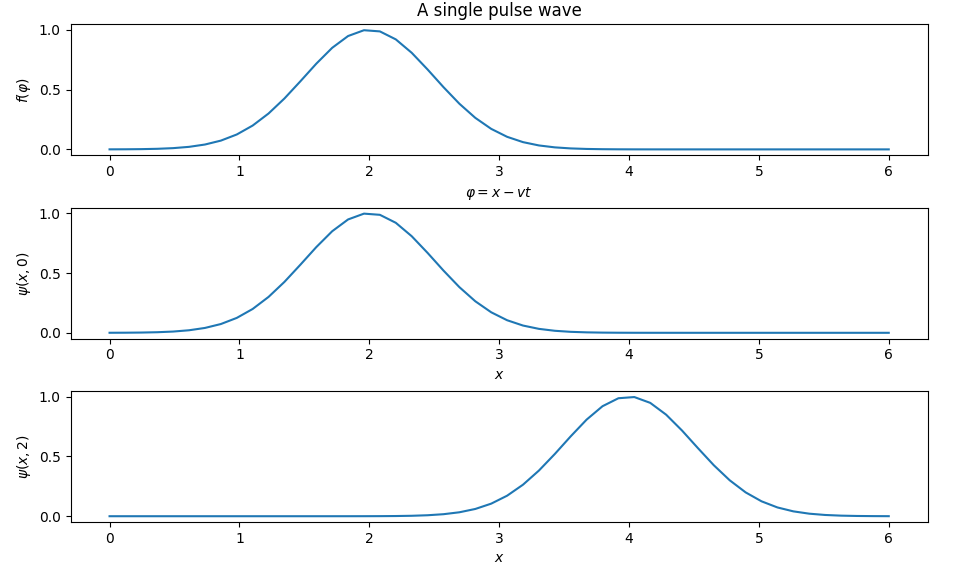
\includegraphics[scale=0.5]{pulse_wave.png}
        \caption{A function \(f\), the wave \(\psi(x, t) = f(x - vt)\) at times \(t = 0, 2\) for \(v = 1\).}
        \label{fig:pulse wave}
    \end{figure}
    The peak of \(f\) in this figure occurs at \(\varphi = x - vt = 2\).
    At \(t = 0\) we have \(\psi(x, 0) = f(x - 0)\) which has a peak at \(x = 2\).
    At \(t = 0\) we have \(\psi(x, 2) = f(x - 1\cdot 2)\) which still has a peak at \(\varphi = 2\) which means the peak is at \(x = 4\).
    We can also view this as a transformation of the original wave as \(x \to x - 2\) represents a translation \(+2\) units in the \(x\) direction.
    
    \subsubsection{Harmonic Wave}
    Often we think of waves as being periodic and repeating regularly.
    Of all the waves of this type the most important are the harmonic waves which are described mathematically by sines and cosines.
    We will see later that through Fourier series we can actually use a superposition of harmonic waves to describe any wave.
    
    The most simple harmonic wave is
    \[\psi(x, t) = A\sin(k(x - vt) - \Phi)\]
    where \(A\) is the amplitude, \(v\) is the velocity, and \(\Phi\) is some constant phase shift.
    The phase of this wave is \(\varphi = k(x - vt) - \Phi\).
    If we consider \(\psi\) at some fixed point as time varies we see it is periodic in time with period \(\tau\).
    We know that \(\sin\) is periodic with period \(2\pi\) so we must have that at \(x = x_0\)
    \[k(x_0 - vt_0) - \Phi - k(x_0 - v(t_0 + \tau)) + \Phi = 2\pi \implies kv = \frac{2\pi}{\tau} = \omega.\]
    \(\omega\) is the temporal angular frequency, or frequency for short.
    Similarly if we consider the wave at \(t = 0\) then we see that it is periodic in space with period \(\lambda\), known as the wavelength.
    Again \(\sin\) is periodic with period \(2\pi\) so
    \[k\lambda = 2\pi \implies k = \frac{2\pi}{\lambda}.\]
    \(k\) is the spatial angular frequency, or wave number for short.
    
    It is common to write waves in a way which explicitly gives \(k\) and \(\omega\), such as
    \[\psi(x, t) = A\sin(kx - kvt - \Phi) = A\sin(kx - \omega t - \Phi).\]
    This is beneficial as it puts space and time on an equal footing.
    We can easily recover \(v = \omega / k\).
    The relationship between spatial and temporal parts is called a \define{dispersion relation}.
    
    Another notational convenience is to use complex exponentials, such as
    \[\psi(x, t) = Ae^{i(kx - \omega t - \Phi)} = A\cos(kx - \omega t - \Phi) + i\sin(kx - \omega t - \Phi).\]
    The complex numbers simplify a lot of calculations but it is the real part of \(\psi\) that corresponds to the physical disturbance.
    
    \subsubsection{Phase Velocity}
    Strictly speaking the velocity of the wave that we have spoken of so far is the \define{phase velocity}.
    It is the velocity of a peak of the wave.
    For example the peak of our sinusoidal wave occurs at phase \(\varphi = \pi / 2\).
    If there is a crest at \((x_1, t_1)\) then we must have
    \[kx_1 - \omega t_1 - \Phi = \frac{\pi}{2}.\]
    At time \(t_1 + \delta t\) the crest must then be at \(x_1 + \delta x\) which satisfies
    \[k(x_1 + \delta x) - \omega(t_1 + \delta t) - \Phi = \frac{\pi}{2}.\]
    Subtracting the first of these from the second we get
    \[k\delta x - \omega\delta t = 0 \implies \frac{\delta x}{\delta t} = \frac{\omega}{k}.\]
    It is this velocity that we refer to when we say the phase velocity.
    Note that we don't have to use a crest here, we could just as well have used a trough or a point of zero displacement or any other condition of constant phase.
    
    \subsection{Waves in Three Dimensions}
    The wave equation generalises to three dimensions as
    \[\laplacian\psi = \frac{1}{v^2}\pdv[2]{\psi}{t},\]
    and the condition \(\psi(x, t) = f(kx - \omega t)\) becomes \[\psi(\vv{r}, t) = f(\vv{k}\cdot\vv{r} - \omega t),\]
    where \(\vv{k}\) is the \define{wave vector}.
    
    \subsubsection{Plane Waves}
    The quantity \(\vv{k}\cdot\vv{r}\) is the displacement in the direction \(\vv{k}\).
    There is a whole plane of points, \(\vv{r}\), which give the same value for \(\vv{k}\cdot\vv{r}\).
    These planes which satisfy \(\vv{k}\cdot\vv{r} = \text{const}\) are called wavefronts.
    These planes have the same phase everywhere on the plane at any given time.
    As well as the shape of the wavefronts we also have to consider the shape of the wave.
    one of the most common plane waves is
    \[\psi(\vv{r}, t) = Ae^{i(\vv{k}\cdot\vv{r} - \omega t - \Phi)}.\]
    
    Three-dimensional waves are hard to draw as we really need four dimensions to draw them, one for each spatial direction and one for the amplitude, even if we fix \(t\) as some constant value.
    Instead we will often consider a two-dimensional wave and use the third dimension for plotting the amplitude.
    For example see figure~\ref{fig:2d wave}.
    \begin{figure}[ht]
        \centering
        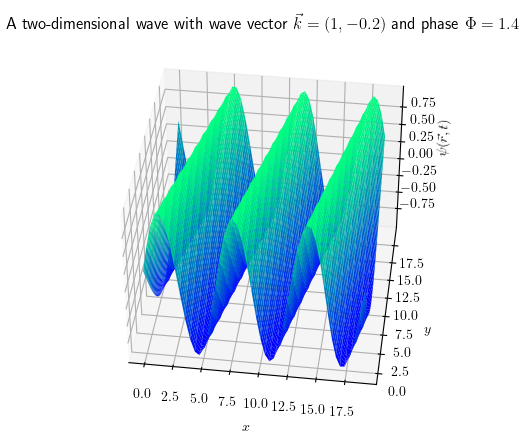
\includegraphics[scale=0.6]{2d_wave.png}
        \caption{A plane wave in two dimensions with \(\vv{k} = (1, -0.2)\) and \(\Phi = 1.4\). The wave is \(\psi(\vv{r}, t) = \exp(i[x - 0.2 y - 1.4])\).}
        \label{fig:2d wave}
    \end{figure}
    
    \subsubsection{Spherical Waves}
    Another common case of three-dimensional waves is something radiating from a point.
    In this case the wavefronts are spherical and we are best to work with spherical coordinates.
    The Laplacian of a central function in spherical coordinates is
    \[\laplacian\psi(r) = \frac{1}{r}\pdv{r}\left(r^2\pdv{\psi}{r}\right) = \pdv[2]{\psi}{r} + \frac{2}{r}\pdv{\psi}{r} = \frac{1}{r}\pdv[2]{r}(r\psi).\]
    Using the last version we find that \(r\psi\) satisfies the one-dimensional wave equation and therefore
    \[\psi(r, t) = \frac{1}{r}f(r - vt).\]
    For example a harmonic spherical wave might be given by
    \begin{equation}\label{eqn:harmonic spherical wave}
        \psi(r, t) = \frac{A}{r}\sin(k(r - vt)).
    \end{equation}
    The factor of \(1/r\) is important.
    It ensures that the intensity of the wave decreases as the wave spreads out.
    Far from the origin a spherical wave will approximate a plane wave.
    This can be seen in figure~\ref{fig:spherical wave approx plane wave}
    \begin{figure}[ht]
        \centering
        \tikzsetnextfilename{spherical-wave-approximates-plane-wave}
        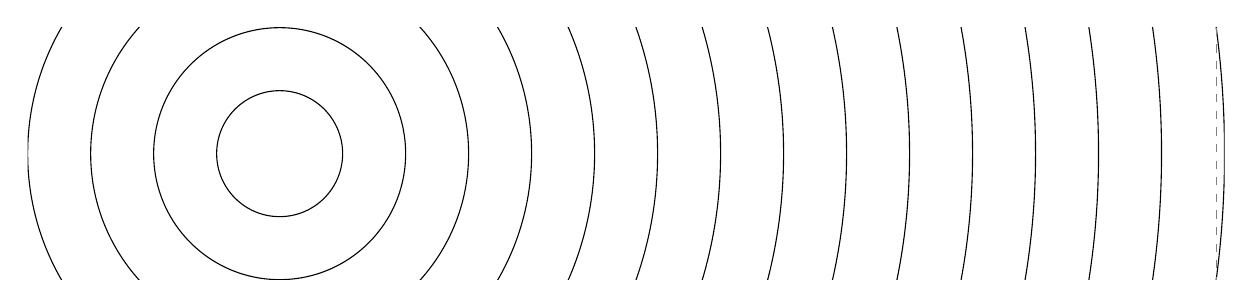
\begin{tikzpicture}
            \begin{scope}[scale=0.8]
                \clip (-3, 0) rectangle (16, 4);
                \foreach \r in {0, ..., 16} {
                    \draw (1, 2) circle[radius=\r];
                }
                \draw[gray, dashed] (15.874, 4) -- (15.874, 0);
            \end{scope}
        \end{tikzpicture}
        \caption{A spherical wave at large distances approximates a plane wave. Notice how at the far right the wavefront is almost parallel to the straight dashed line.}
        \label{fig:spherical wave approx plane wave}
    \end{figure}

    \section{Electromagnetic Waves}
    \subsection{Energy Density and Optical Intensity}
    Recall that the Poynting vector is defined as
    \[\vv{S} = \frac{1}{\mu_0}\vv{E}\times\vv{B},\]
    and that the energy density of an electromagnetic wave in a vacuum is
    \[u = \frac{1}{2}\varepsilon_0E^2 + \frac{1}{2\mu_0}B^2 \varepsilon_0E^2.\]
    For a harmonic wave polarised in the \(x\) direction (that is \(\vv{E}\propto\ve{x}\) so \(\vv{B}\propto\ve{y}\) and \(\vv{k}\propto\ve{z}\)) the energy density is
    \[u = \varepsilon_0E^2 = \varepsilon_0 E_0^2\cos^2(kz - \omega t - \Phi)\]
    and the Poynting vector is
    \[\vv{S} = c\varepsilon_0E_0^2\cos^2(kz - \omega 6 - \Phi)\ve{z} = cu\ve{z}.\]
    For an optical wave \(\omega \approx \SI{e15}{\second^{-1}}\).
    It is therefore not possible to measure an instantaneous value of \(\vv{E}\), \(\vv{B}\), \(\vv{S}\), or \(u\).
    Instead we can measure the rate of energy transferred over a long period.
    This corresponds to averaging over many periods.
    We define the \define{intensity} as
    \[I = \expected{S} = c\varepsilon_0\expected{E}\]
    where \(\expected{f}\) denotes an average of \(f\) over many periods which can be computed as
    \[\expected{f} = \frac{1}{t_{\max}} \int_0^{t_{\max}}f(t)\dd{t}\]
    where \(t_{\max}\gg T\) where \(T = 2\pi/\omega\) is the period of \(f\).
    
    \subsection{Violation of Newton's Third Law?}
    Consider the two charges shown in figure~\ref{fig:violation of N3 setup}.
    \begin{figure}[ht]
        \centering
        \tikzsetnextfilename{moving-charges-violate-N2}
        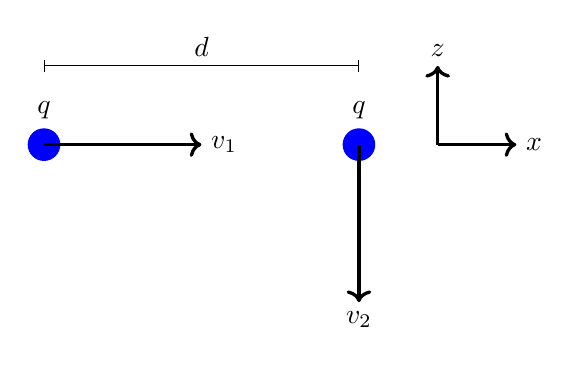
\begin{tikzpicture}
            \tikzstyle{charge} = [fill=blue, color=blue]
            \tikzstyle{vector} = [very thick, ->]
            \draw[charge] (0, 0) circle[radius=0.2cm];
            \draw[charge] (4, 0) circle[radius=0.2cm];
            \node[above] at (0, 0.2) {\(q\)};
            \node[above] at (4, 0.2) {\(q\)};
            \draw[vector] (0, 0) -- (2, 0);
            \draw[vector] (4, 0) -- (4, -2);
            \node[right] at (2, 0) {\(\vv{v_1}\)};
            \node[below] at (4, -2) {\(\vv{v_2}\)};
            \draw[vector] (5, 0) -- (5, 1);
            \draw[vector] (5, 0) -- (6, 0);
            \node[above] at (5, 1) {\(z\)};
            \node[right] at (6, 0) {\(x\)};
            \draw[|-|] (0, 1) -- (4, 1);
            \node[above] at (2, 1) {\(d\)};
        \end{tikzpicture}
        \caption{Two moving charges.}
        \label{fig:violation of N3 setup}
    \end{figure}
    It shows two charges of charge \(q\).
    One is moving horizontally along the \(x\)-axis with velocity \(\vv{v_1}\) and the other is moving in the \(-z\) direction with velocity \(\vv{v_2}\).
    Suppose that \(v_1 = v_2 = v\).
    The force due to the electric field from charge 1 on charge 2 is
    \[\vv{F_{E2}} = \frac{q^2}{4\pi\varepsilon_0d^2}\ve{x}.\]
    Similarly the force due to the electric field from charge 2 on charge 1 is
    \[\vv{F_{E1}} = -\frac{q^2}{4\pi\varepsilon_0d^2}\ve{x}.\]
    These forces are equal and opposite as Newton's third law would predict.
    
    The force due to the magnetic field from charge 1 on charge 2 is
    \[\vv{F_{B2}} = q\vv{v_2}\times\vv{B_1} = q\vv{v_2}\times\left[\frac{q}{4\pi\varepsilon_0c^2}\frac{\vv{v_1}\times\vv{r_2}}{r_2^3}\right] = \vv{0}.\]
    This is \(\vv{0}\) since \(\vv{r_2}\), the vector from charge 1 to charge 2, is parallel to \(\vv{v_1}\).
    The force due to the magnetic field form charge 2 on charge 1 is
    \[\vv{F_{B1}} = q\vv{v_1}\times\vv{B_2} = q\vv{v_1} \times \left[\frac{q}{4\pi\varepsilon_0c^2}\frac{\vv{v_2}\times\vv{r_1}}{r_1^3}\right]\ne \vv{0}.\]
    So the forces due to the magnetic fields are \emph{not} equal and opposite.
    This seems to violate Newton's third law.
    In the next system we will see why this is.
    
    \subsection{Radiation Pressure}
    Light incident on a positive charge, \(q\), at some moment when \(\vv{E}\) is in the positive \(x\) direction will initiate movement of the charge in the positive \(x\) direction doing work at a rate
    \[\dv{W}{t} = \vv{v}\cdot\vv{F_E} = v_xqE_x.\]
    At this point the charge is moving and therefore experiences a force due to the magnetic component of the light.
    At the same moment this component is in the positive \(y\) direction and the force is
    \[\vv{F_B} = q\vv{v}\times\vv{B} = qv_x\ve{x}\times B_y\ve{y} = qv_xB_y\ve{z}.\]
    At a later time when \(\vv{E}\) is in the negative \(x\) direction the rate of work that \(\vv{E}\) does will be
    \[\dv{W}{t} = \vv{v}\cdot\vv{F_E} = -v_xqE_x.\]
    At the same moment \(\vv{B}\) will be in the negative \(y\) direction and the charge will be moving now in the negative \(x\) direction so the force due to the magnetic field is
    \[\vv{F_B} = q\vv{v}\times\vv{B} = q(-v_x\ve{x})\times(-B_y\ve{y}) = qv_xB_y\ve{z}.\]
    Notice that one period the average force due to \(\vv{E}\) is 
    \[\expected{\vv{F_E}} = q\expected{\vv{E}} = \vv{0}.\]
    However the average net force is
    \[\expected{\vv{F}} = \expected{\vv{F_E} + \vv{F_B}} = \expected{\vv{F_B}} = q\expected{v_xB_y}\ve{z} = \frac{q}{c}\expected{v_xE_x}\ve{z},\]
    using the fact that for an electromagnetic wave \(B_y = E_x/c\).
    From this we see that there is a net force which does work at a rate
    \[\expectedResize{\dv{W}{t}} = \expected{\vv{v}\cdot\vv{F}} = \expected{\vv{v}\cdot(\vv{F_E}\cdot\vv{F_B}} = \expected{\vv{v}\cdot\vv{F_E}} = q\expected{v_xE_x},\]
    where we have used the fact that \(\vv{v}\cdot\vv{F_B} = \vv{v}\cdot(\vv{v}\times\vv{B}) = 0\).
    We see that there is a net gain in energy while the light is incident on the charge.
    Notice that
    \[\expectedResize{\dv{W}{t}}\ve{z} = c\expected{\vv{F}} = \expectedResize{\dv{\vv{p}}{t}}.\]
    So there is a net gain in momentum.
    This gain of momentum is inversely proportional to \(c\) so is often too small to notice.
    The pressure due to this force is called \define{radiation pressure}.
    For example on Earth the energy density from solar radiation is approximately \(\SI{1}{\kilo\watt.\meter^-2}\).
    This is an appreciable amount of energy, the sun feels warm.
    However the radiation pressure is then on the order of \(\SI{e-6}{\pascal}\) which is 11 orders of magnitude smaller than atmospheric pressure.
    
    While this effect is small it is still important.
    For example there have been a few space probes that use the radiation pressure of the sun to accelerate.
    To do this they use large sails to maximise the are over which sunlight is incident.
    Even traditionally driven probes have to account for the radiation pressure changing their course slightly.
    
    This effect also explains the seeming violation of Newton's third law earlier.
    If we properly account for the radiation pressure then we will find that Newton's third law is not violated.
    
    We saw with radiation pressure that the momentum is equal to the energy divided by \(c\).
    If we consider for a moment quantum mechanics then we have
    \[p = \frac{h}{\lambda}\qquad \text{and} E = hf = \frac{hc}{\lambda} = pc \implies p = \frac{E}{c}.\]
    If instead we consider special relativity then we have
    \[E^2 = m^2c^4 + p^2c^2\]
    if \(m = 0\) then we have
    \[E = pc \implies p = \frac{E}{c}.\]
    So we have agreement between electromagnetism, quantum mechanics, and special relativity as to \(p = E/c\).
    
    One experimental verification of radiation pressure comes from Compton scattering.
    This is a process by which an incoming photon of wavelength \(\lambda_i\) hits an electron which deflects away at angle \(\varphi\) and the photon deflects at angle \(\vartheta\).
    The wavelength of the scattered photon is \(\lambda_f\).
    It can be shown that
    \[\lambda_f - \lambda_i = \Delta \lambda = \frac{h}{m_ec}(1 - \cos\vartheta).\]
    Since some momentum must be transferred to the electron the momentum of the photon must decrease and therefore the wavelength changes.
    
    \section{Dipole Radiation}
    \subsection{Light From Maxwell's Equations}
    Recall that we can combine Maxwell's equations to get the wave equations
    \[\laplacian\vv{E} = \mu_0\varepsilon_0 \partial_t^2\vv{E}, \qquad\text{and}\qquad \laplacian\vv{B} = \mu_0\varepsilon_0\partial_t\vv{B}.\]
    We see that each component of the electric and magnetic fields must satisfy the three-dimensional wave equation for a wave travelling at speed \((\mu_0\varepsilon_0)^{-1/2}\), which is the speed of light.
    This was one of the facts that originally convinced Maxwell that light could be explained as an electromagnetic phenomenon.
    
    Suppose we have an electromagnetic wave which propagates such that
    \[E_i(\vv{r}, t) = f(\vv{k}\cdot\vv{r} - \omega t).\]
    These are plane waves propagating along \(\vv{k}\).
    Now we choose \(\ve{z}\) to be the same direction as \(\vv{k}\) so that \(E_i(\vv{r}, t) = f(kz - \omega t)\).
    We see that
    \[\div\vv{E} = \partial_z E_z\]
    if we further assume that the wave is propagating in free space then we have \(\div\vv{E} = 0 = \partial_z E_z\).
    This means that \(\vv{E}\) doesn't oscillate in the direction of propagation meaning that it is a transverse wave.
    Suppose at some point \(\vv{E}\) is aligned with \(\ve{x}\).
    Then We must have \(\vv{B}\) parallel to \(\ve{y}\) as we know that it is perpendicular to \(\vv{E}\).
    
    Suppose
    \[\vv{E} = E_x(\vv{r}, t)\ve{x} = E_{x0}\cos(kz - \omega t - \Phi)\ve{x}.\]
    That is \(\vv{E}\) is a harmonic wave polarised in the \(x\) direction.
    We then find from Faraday's law that
    \[-\partial_t B_y = \partial_z E_x = -E_{x0}k\sin(kz - \omega t - \Phi).\]
    From this we have
    \[B_y = E_{x0}k \int \sin(kz - \omega t - \Phi) \dd{t} = E_{x0}\frac{k}{\omega}\cos(kz - \omega t - \Phi) = \frac{1}{c}E_{x0}\cos(kz - \omega t - \Phi) = \frac{E_x}{c}.\]
    So the \(\vv{B}\) oscillates perpendicular to \(\vv{E}\) and has a magnitude \(B = E/c\).
    
    \subsection{Dipole Radiation}
    Suppose we have an atom at rest.
    If we displace the electron cloud slightly we will have an effective dipole.
    This dipole turns out to be critical to how light interacts with matter.
    Suppose that we distort an atom to create a dipole moment \(\vv{p_0}\).
    Approximating this as an ideal dipole the field we expect is
    \[E_r = \frac{2p_0\cos\vartheta}{4\pi\varepsilon_0r^3}, \qquad\text{and}\qquad E_\vartheta = \frac{p_0\sin\vartheta}{4\pi\varepsilon_0r^3}.\]
    Due to rotational symmetry about \(\vv{p_0}\) we expect that there will be no \(\varphi\) dependence of the field.
    
    If we slightly distort the dipole and then allow it to change freely then to second order we expect harmonic oscillation so we expect the dipole to vary as
    \[\vv{p}(t) = \vv{p_0}\cos(\omega t).\]
    However we cannot use this new dipole in the equations for a dipole field.
    The problem is that these equations assume the dipole is static, which is no longer the case.
    The reason this assumption is necessary is the finite speed of light.
    While the dipole oscillates it takes time for the change in the field to propagate and by the time it has the dipole is different again.
    There is a time lag in the response to the oscillation and the lag increases with distance.
    
    \subsubsection{Retarded Time}
    The solution to the dipole field of an oscillating dipole uses a concept called \define{retarded time}.
    The retarded time at a distance \(x\) from an accelerating charge is \(t' = t - x/c\) where \(t\) is the actual time.
    We use square brackets, \([\cdot]\), to denote a quantity that is to be calculated at the retarded time.
    For example if \(a = a(t)\)  is the acceleration of a charge then \([a] = a(t')\) is the acceleration of the charge at the retarded time.
    If we have a single charge accelerating along the \(z\)-axis then it can be shown that the electric field at some distance, \(x\), along the \(x\)-axis at time \(t\) is
    \[\vv{E}(x, y=0, z=0, t) = \ve{x}\frac{q}{4\pi\varepsilon_0 x^2} - \ve{z}\frac{q[a]}{4\pi\varepsilon_0 xc^2}.\]
    The first term is the normal Coulomb term due to the presence of the charge.
    The second term, called the retarded term, is due to the accelerating charge causing a changing magnetic field which in turn causes an electric field.
    We see that in the limit \(c\to\infty\) the retarded term disappears which makes sense since the retarded term only appears due to the fact that \(c\) is \emph{not} infinite.
    In the limit \(x\to\infty\) the retarded term dominates.
    
    \subsubsection{Full Dipole Radiation Equations}
    It can be shown that the electric and magnetic fields for a time dependent dipole, with magnitude \(p(t)\) oriented along the \(z\)-axis, are given by
    \begin{align*}
        E_r &= \frac{2}{4\pi\varepsilon_0} \left(\frac{[p]}{r^3} + \frac{[\inlinedv{p}{t}]}{cr^2}\right),\\
        E_\vartheta &= \frac{1}{4\pi\varepsilon_0} \left(\frac{[p]}{r^3} + \frac{[\inlinedv{p}{t}]}{cr^2} + \frac{[\inlinedv[2]{p}{t}]}{c^2r} \right) \sin\vartheta,\\
        B_\varphi &= \frac{1}{4\pi\varepsilon_0} \left(\frac{[\inlinedv{p}{t}]}{c^2r^2} + \frac{[\inlinedv[2]{p}{t}]}{c^3r}\right) \sin\vartheta
    \end{align*}
    and
    \[E_\varphi = B_r = B_\vartheta = 0.\]
    The terms including a factor of \([p]\) are the fields due to the static field.
    Again if we take the limit \(c\to\infty\) then this reduces to the equations for a static dipole as propagation time becomes zero.
    Far from the dipole the \(1/r^3\) terms dominate and we have
    \[E_r\approx 0, \qquad E_{\vartheta} \approx \frac{1}{4\pi\varepsilon_0} \frac{[\inlinedv[2]{p}{t}]}{c^2r}\sin\vartheta, \qquad\text{and}\qquad B_\varphi \approx \frac{1}{4\pi\varepsilon_0} \frac{[\inlinedv[2]{p}{t}]}{c^3r}\sin\vartheta.\]
    These equations are much simpler and we will work with them.
    We see that \(B = E/c\) as we would expect and also that \(\vv{E}\) and \(\vv{B}\) are perpendicular to each other and to \(\ve{r}\) which is the propagation direction.
    The two fields are in phase and the \(\sin\vartheta\) term means that the fields are strongest around the `equator' of the dipole and are zero along the \(z\) axis.
    The \(\vv{B}\) field is azimuthal (in the \(\ve{\varphi}\) direction) which is also the case with a current carrying wire along the \(z\)-axis.
    Far from the origin \(\vv{E}\) and \(\vv{B}\) have a form similar to  equation~\ref{eqn:harmonic spherical wave} which means that they look like harmonic spherical waves with an extra \(\sin\vartheta\) term which decreases the magnitude towards the poles.
    As one last observation note that the magnitude of the pointing vector is \(S = \abs{\mu_0^{-1}\vv{E}\times\vv{B}} \propto 1/r^2\), so intensity decays as \(I = \expected{S} \propto 1/r^2\) as we would expect for light which famously follows an inverse square law for intensity.
    
    All of these points hold for the approximate version of the equations `far' from the dipole.
    So when is this a good approximation?
    What counts as far?
    The answer turns out to be that far is not very far at all.
    In fact the \(1/r\) terms dominate enough that the approximation is valid for \(r\) being only a few wavelengths which is very small.
    Since the approximation is valid so close and we aren't doing quantum mechanics we really needn't consider anything other than the far field approximation here.
    
    \section{Electromagnetic Waves in Dielectrics}
    An electromagnetic field in a dielectric with permittivity \(\varepsilon = \varepsilon_0\varepsilon_r\) and permeability \(\mu = \mu_0\mu_r\) can be shown to lead to the wave equations
    \[\laplacian\vv{E} = \varepsilon\mu\partial_t^2\vv{E}, \qquad\text{and}\qquad \laplacian\vv{B} = \varepsilon\mu \partial_t^2\vv{B}.\]
    We assume that the dielectric is linear, isotropic and homogenous.
    That is the polarisation is linearly proportional to the applied electric field and the material properties are the same in all directions and everywhere in space.
    
    These corresponds to waves with phase velocity
    \[v_p = \frac{\omega}{k} = \frac{1}{\sqrt{\mu\varepsilon}} = \frac{c}{\sqrt{\mu_r\varepsilon_r}}.\]
    We see that the speed of light in the medium is attenuated by a factor of \(1/\sqrt{\mu_r\varepsilon_r}\).
    We call this factor, \(n = \sqrt{\mu_r\varepsilon_r}\), the \define{refractive index}.
    For a material that is not a ferromagnet we find that \(\mu_r \approx 1\) and so \(n = \sqrt{\varepsilon_r}\) is usually a good approximation for our purposes and
    \[v_p = \frac{c}{\sqrt{\mu_r\varepsilon_r}} = \frac{c}{n} \approx \frac{c}{\sqrt{\varepsilon_r}}.\]
    
    Recall that an electric field causes a polarisation \(\vv{P} = \chi_E\varepsilon_0\vv{E}\) where \(n^2 \approx \varepsilon_r = 1 + \chi_E\).
    Therefore if we can calculate the polarisation, \(\vv{P}\), we can find \(\varepsilon_r\) and from this we can find the refractive index, \(n\).
    We can calculate \(\vv{P}\) from the polarisation of a single molecule, \(\vv{p}\), and then \(\vv{P} = N\vv{p}\) where \(N\) is the number density of molecules.
    
    \subsection{Snell's Law Derivation From Fermat's Principle}\label{sec:snell's law fermat's principle}
    Fermat's principle of stationary time states that a light ray travelling between two points takes a path such that the time taken is stationary with respect to variations in the path.
    Roughly speaking this means that a slight variation in the path to a nearby path will cause, at most, second order changes in the traversal time.
    While the principle simply states `stationary' it is often assumed that the time taken is in fact minimal.
    After all there is an infinite number of paths that take arbitrarily long to reach the point.
    
    Fermat's principle makes no assumptions about light as an electromagnetic wave but we will see that it leads to many correct predictions.
    For example, we will use it here to derive Snell's law.
    This principle is the basis of geometric optics, which is the field of optics where light is treated as a ray and its path through space calculated based on various rules for how this ray interacts with the mediums it travels through.
    
    \begin{figure}[ht]
        \centering
        \tikzsetnextfilename{refraction-again}
        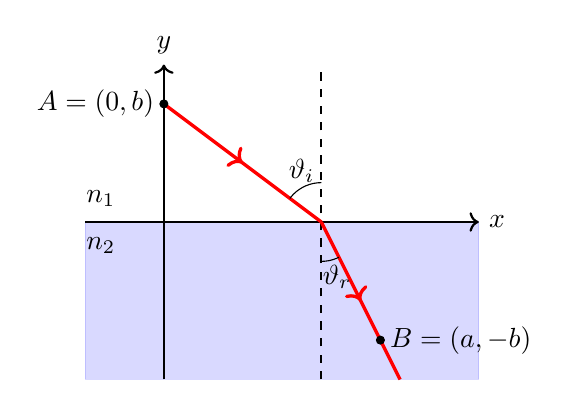
\begin{tikzpicture}
            \tikzstyle{glass} = [fill=blue!50, opacity=0.3, color=blue!50]
            \tikzstyle{ray} = [very thick, red, decoration={markings, mark=at position 0.5 with {\arrow{>}}}, postaction={decorate}]
            \draw[glass] (-2, -2) rectangle (3, 0);
            \draw[dashed, thick] (1, -2) -- (1, 2);
            \draw[thick, ->] (-1, -2) -- (-1, 2) node[above] {\(y\)};
            \draw[thick, ->] (-2, 0) -- (3, 0) node[right] {\(x\)};
            \node at (-1.8, 0.3) {\(n_1\)};
            \node at (-1.8, -0.3) {\(n_2\)};
            \draw[ray] (-1, 1.5) -- (1, 0);
            \draw[ray] (1, 0) -- (2, -2);
            \draw[fill=black] (1.75, -1.5) circle[radius=0.05cm] node[right] {\(B = (a, -b)\)};
            \draw[fill=black] (-1, 1.5) circle[radius=0.05cm] node[left] {\(A = (0, b)\)};
            \begin{scope}
                \clip (1, 0) -- (1, 2) -- (-1, 1.5) -- (1, 0);
                \draw (1, 0) circle[radius=0.5cm];
            \end{scope}
            \node at (0.75, 0.65) {\(\vartheta_i\)};
            \begin{scope}
                \clip (1, 0) -- (2, -2) -- (1, -2) -- (1, 0);
                \draw (1, 0) circle[radius=0.5cm];
            \end{scope}
            \node at (1.2, -0.7) {\(\vartheta_r\)};
        \end{tikzpicture}
        \caption{Light being refracted at the boundary between two media.}
        \label{fig:snell's law by fermat's principle}
    \end{figure}
    Consider light travelling from point \(A\) to \(B\) and along the way it changes from one medium with refractive index \(n_1\) to another with refractive index \(n_2\).
    Within a medium the only stationary path is a straight line, which is what we expect.
    What we don't know is what angles the light will meet the medium at.
    It is traditional to consider the angle to the normal with the incoming angle being called the angle of incidence, \(\vartheta_i\), and the outgoing angle being called the angle of refraction, \(\vartheta_r\)
    Set up coordinates as in figure~\ref{fig:snell's law by fermat's principle}.
    Notice that the diagram shows \(\vartheta_r < \vartheta_i\) but this is not necessarily the case.
    We can fix both angles by choosing the point \(C = (x, 0)\), along the \(x\)-axis at which the light passes from one medium to the other.
    
    The total time taken for the light to travel from \(A\) to \(B\) is \(T = T_1 + T_2\) where \(T_1\) is the time to travel the path in medium 1 and \(T_2\) is the time to travel the path in medium 2.
    Using the fact that the speed of light in a given medium is \(c/n_i\) and the fact that time is distance over speed we have
    \begin{align*}
        T &= T_1 + T_2\\
        &= \frac{\abs{\overrightarrow{AC}}}{c/n_1} + \frac{\abs{\overrightarrow{CB}}}{c/n_2}\\
        &= \frac{\sqrt{b^2 + x^2}}{c/n_1} + \frac{\sqrt{b^2 + (a - x)^2}}{c/n_2}.
    \end{align*}
    For the time to be stationary we require
    \[\dv{T}{x} = 0.\]
    Calculating the derivative we have
    \[\dv{T}{x} = \frac{n_1}{c} \frac{x}{\sqrt{b^2 + x^2}} - \frac{n_2}{c} \frac{a - x}{\sqrt{b^2 + (a - x)^2}} = 0.\]
    Hence
    \[\frac{n_1x}{\sqrt{b^2 + x^2}} = \frac{n_2(a - x)}{\sqrt{b^2 + (a - x)^2}}.\]
    Now simply applying the definition of \(\sin\vartheta\) as opposite over hypotenuse we have
    \[n_1\sin\vartheta_i = n_2\sin\vartheta_r.\]
    This is \define{Snell's law} of refraction.
    This derivation was based on geometric optics and Fermat's principle of stationary time.
    In later sections we will derive this same result with Huygen's principle and full electromagnetic theory.
    
    \subsection{Polarisation and Refractive Index}
    We can use Snell's law to measure the refractive index of a material.
    If we do this we find that \(n\) decreases as frequency decreases.
    If we ask why this is the first thing we may think of is since \(n^2 = \varepsilon_r\) is related to polarisation the polarisation must also be frequency dependent.
    To find out why we may ask what it is that causes polarisation.
    There are three components that we might consider:
    \begin{itemize}
        \item The orientation of polar molecules leads to polarisation when the molecules align their dipoles with the electromagnetic field.
        This requires the entire molecule to rotate so happens on the time scales of rotational frequencies.
        For example in water it takes approximately \SI{10}{\pico\second}.
        \item The polarisation of ions leads to polarisation when the molecules distort to align the resulting dipole with the electromagnetic field.
        This requires only part of the molecule to move and so happens on the time scale of vibrational frequencies.
        For example in water it takes approximately \SI{1}{\pico\second}.
        \item The polarisation of non-polar molecules leads to polarisation when the electron cloud is distorted to create a dipole aligned with the electromagnetic field.
        This requires only electrons to move and so happens on very short time scales of about \SI{1}{\femto\second}.
    \end{itemize}
    From all of these mechanisms the key point is that polarisation is not instantaneous.
    If the field is oscillating back and forth we expect the polarisation to lag behind.
    How much it lags behind will depend on how fast the field oscillates.
    There si just one problem.
    This explanation would lead to us expecting that refractive index decreases as frequency increases.
    This is the exact opposite of what we see experimentally.
    To find out why this isn't what happens we will need a more careful treatment of the oscillation of the dipoles with changes in the field.
    This is what we will do in the next section.
    
    \section{Oscillator Model}
    For simplicity we assume that interactions between electrons are negligible and that we can model the electron cloud as simply being stuck in a potential well caused by the Coulomb interaction with the nucleus.
    If we expand this potential to second order then, by definition, we have a quadratic potential.
    We can therefore model the motion of the electron cloud as a harmonic oscillator obeying
    \[\massElectron \dv[2]{x}{t} = \chargeElectron E_x - \massElectron\omega_0^2x - \massElectron\gamma \dv{x}{t}.\]
    Here \(\massElectron\) and \(\chargeElectron\) are the mass and charge of the electron cloud, \(x\) is the displacement of the centre of mass of the electron cloud from the centre of mass of the atom and \(\gamma\) is a damping coefficient.
    We also assume that any radiation is \(x\) polarised for simplicity so
    \[E_x = E_0\cos(\omega t).\]
    If we include this we then have a damped harmonic oscillator with resonant frequency \(\omega\) being driven at frequency \(\omega\).
    
    In the undamped (\(\gamma = 0\)) case this has the solution
    \[x(t) = x_0\cos(\omega t) = \frac{\chargeElectron/\massElectron}{\omega_0^2 - \omega^2}E_i\cos(\omega t) = \frac{\chargeElectron/\massElectron}{\omega_0^2 - \omega^2}E(t).\]
    Notice that this motion of the electron cloud sets up a dipole with dipole moment \(p = \chargeElectron x\).
    Notice also that \(\chargeElectron < 0\) and the dipole vector, \(\vv{p}\), is conventionally defined to point from negative to positive, meaning that \(\vv{p}\) points in the opposite direction to \(\vv{x}\).
    From this we can draw conclusions based on two different cases for the values of \(\omega\) and \(\omega_0\):
    \begin{itemize}
        \item For the case of \(\omega < \omega_0\), i.e. below the natural frequency, the electron shell oscillates exactly \(\pi\) out of phase with the electric field, \(\vv{E}(t)\).
        That is \(\vv{x}\) points in the opposite direction to \(\vv{E}\) and so \(\vv{p}\) points in the same direction to \(\vv{E}\).
        
        \item For the case of \(\omega > \omega_0\), i.e. above the natural frequency, the electron cloud oscillates exactly in phase with the electric field, \(\vv{E}(t)\).
        That is \(\vv{x}\) points in the same direction as \(\vv{E}\) and so \(\vv{p}\) points in the opposite direction to \(\vv{E}\).
    \end{itemize}
    We can use the solution for \(x(t)\) to find the atomic dipole moment, \(\vv{p_{\mathrm{atom}}}\) and the polarisation of the atom, which is simply the dipole moment per unit volume.
    From this we can calculate the refractive index:
    \begin{align*}
        n^2 &= \varepsilon_r\\
        &= 1 + \frac{P}{\varepsilon_0E}\\
        &= 1 + \frac{Np_{\mathrm{atom}}}{\varepsilon_0E}\\
        &= 1 + \frac{N\chargeElectron x}{\varepsilon_0E}\\
        &= 1 + \frac{N\chargeElectron^2}{\varepsilon_0\massElectron (\omega_0^2 - \omega^2)}
    \end{align*}
    where \(N\) is the number density (i.e. the number of atoms per unit volume).
    
    This is a simple model so it won't give exactly the right solution.
    In particular it has the following shortcomings:
    \begin{itemize}
        \item In reality there won't be one single resonant frequencies but different components of motion will have different resonant frequencies, \(\omega_{0i}\), and we will have to sum over these.
        
        \item We ignore the interaction between atoms and in particular the effect that atomic dipole has on its neighbours.
        This can be accounted for with something called the Claussius--Mossotti correction but we won't take it into account.
        
        \item There is a singularity at \(\omega = \omega_0\).
    \end{itemize}
    
    In the case where we have non-zero damping the mathematics is harder but we can still find a solution.
    The correct damping regime to consider is light damping where \(0 < \gamma \ll 1/(2\omega_0)\).
    Recall that \(\gamma = 2\omega_0\) leads to critical damping.
    For non-zero damping the initial displacement at \(t = 0\) has explicit \(\omega\) dependence and a phase shift as well.
    The solution turns out o be of the form \(x = x_0\cos(\omega t + \Phi)\) leading to an atomic dipole of the form
    \[p_x = \chargeElectron x = p_0\cos(\omega t + \Phi)\]
    which can be shown to give solutions of the form
    \[p_0(\omega) = \chargeElectron x_0(\omega) = \frac{\chargeElectron^2 E_0/\massElectron}{\sqrt{(\omega_0^2 - \omega^2)^2 + \gamma^2\omega^2}}\]
    and
    \[\Phi = \arctan\left[ \frac{-\gamma\omega}{\omega_0^2 - \omega^2} \right].\] 
    We can solve this for \(x\) and it is easier to do this using complex exponentials for trig and we simply implicitly take the real part when necessary.
    Using \(x = x_0\exp[-i(\omega t + \Phi)]\) we find that
    \[x(\omega) = x_0e^{-i(\omega t + \Phi)} = x_0e^{-i\Phi}e^{-i\omega t} = \left[ \frac{\chargeElectron E_0/\massElectron}{\omega_0^2 - \omega^2 - i\gamma\omega} \right]e^{-i\omega t}\]
    and the dipole moment is then
    \[p_x(\omega) = \frac{\chargeElectron^2 E_x/\massElectron}{\omega_0^2 - \omega^2 - i\gamma \omega}.\]
    We then have
    \begin{equation}\label{eqn:epsilon r oscillator model}
        \varepsilon_r = \varepsilon_r' + i\varepsilon_r'' = 1 + \frac{N\chargeElectron^2}{\varepsilon_0\massElectron (\omega_0^2 - \omega^2 - i\gamma\omega)}
    \end{equation}
    where \(\varepsilon_r'\) and \(\varepsilon_r''\) are the real and imaginary components of \(\varepsilon_r\).
    Using a similar notation for the refractive index, \(n = n' + in''\) we have
    \[\varepsilon_r = n^2 \implies \varepsilon_r' = n'{^2} - n''{^2}, \qquad\text{and}\qquad \varepsilon_r'' = 2n'n''.\]
    Since \(\varepsilon_r\) depends on the frequency, \(\omega\), of the radiation we find that the refractive index also depends on the frequency of the radiation meaning that different colours of light are diffracted/refracted/slowed down by a different amount.
    We can also replace \(\omega_0^2\) with \(\omega_{01}^2 + \omega_{02}^2 + \dotsb\) where \(\omega_{0i}\) are the relevant natural frequencies of the oscillations.
    
    A few features of this new equation show us that it is a good model or raise some more questions:
    \begin{itemize}
        \item If \(\gamma \ne 0\) then we don't have any singularities, even at \(\omega = \omega_0\).
        
        \item The real part of the refractive index, \(n'\), increases with the frequency as \(\omega\) becomes closer to \(\omega_{0i}\) which is what we observe experimentally.
        
        \item Ignoring increases for \(\omega \approx \omega_{0i}\) we have a general decreasing trend in \(n'\) with \(\omega\).
        
        \item For \(\omega > \max\{\omega_i\}\) we have \(n' < 1\) which means that light at these frequencies travels faster than \(\SI{3e8}{\metre.\second^{-1}}\).
        This seems initially like it breaks the rules of special relativity until you recall that the speed of light applies only in a vacuum.
        
        \item Using this model we can measure refractive index dependent things at some frequencies and extrapolate to other frequencies.
    \end{itemize}

    \subsection{Interpreting the Oscillator Model}
    Consider the case of a free electron.
    This corresponds to setting \(\omega_0 = 0\) and so \(\omega_0 < \omega\) which we saw in the previous section meant that the electron oscillates in phase with \(\vv{E}\).
    This initially seems incorrect as the electron has a negative charge and so should move in the \emph{opposite} direction to \(\vv{E}\).
    This would indeed be the case if \(\vv{E}\) was constant, but it isn't.
    The \emph{acceleration} of the electron is what must be in the opposite direction of \(\vv{E}\).
    The displacement is then given by integrating twice and integrating a sinusoid twice gives, up to a positive constant factor, the same sinusoid back but negative.
    So the acceleration is in the opposite direction to \(\vv{E}\) but the position is in the same direction as \(\vv{E}\).
    
    If instead \(\vv{E}\) is static, or equivalently \(\omega = 0\), then the electron is displaced in the opposite direction to \(\vv{E}\) which agrees with the case of \(\omega < \omega_0\) (even though \(\omega = \omega_0 = 0\)).
    
    For the case of \(\omega \approx \omega_0\) we have a large spike in amplitude.
    In the case of the undamped oscillator this is a singularity and the amplitude becomes infinite.
    In the lightly damped case the amplitude is finite but still much larger than in other regions.
    This is due to resonance, recall that a harmonic oscillator has its maximum amplitude at some resonant frequency, \(\omega_r\), which is just slightly lower than \(\omega_0\).
    
    Consider the case of very light damping such that \(\gamma\) becomes infinitesimal.
    In this case the imaginary part of \(x\) or \(\varepsilon_r\) becomes a delta distribution at \(\omega_0\) and the real part becomes discontinuous.
    This is because there is no limit on vibration amplitude in this mathematical model.
    In a real material there is damping as oscillating dipoles will lose energy due to random thermal collisions.
    The dipoles will also re-radiate energy.
    This gives a physical significance the the complex parts of \(\varepsilon_r\) and \(n\) which up until now we have treated purely as a mathematical convenience.
    These terms correspond to how much a given frequency is absorbed by the medium.
    For example glass has \(\omega_0 \approx \SI{e6}{\radian.\second^{-1}}\), which corresponds to light in the UV region of the spectrum.
    Glass also strongly absorbs UV radiation at this frequency which corresponds to the high peak at this point in \(\varepsilon_r''\) and \(n''\).
    
    For low frequencies, \(\omega \ll \omega_0\), \(\tan\Phi\) is small and negative, which means that \(\Phi\) is small and negative.
    This means that the oscillations have a negligible phase lag.
    For \(\omega = \omega_0\) we have \(\Phi = -\pi/2\) and for \(\omega \gg \omega_0\) we \(\Phi\) approaches \(-\pi\).
    So the phase lag increases as \(\omega\) increases.
    This corresponds to \(\varepsilon_r\) dropping from greater than 1 for \(\omega \ll \omega_0\) to being smaller than 1 for \(\omega \gg \omega_0\).
    At low frequencies the polarisation of matter opposes the changing electric field and at higher frequencies it reinforces the changing field.
    
    
    \section{Huygens' Principle and Colour}
    \subsection{Huygens' Principle}\label{sec:huygens principle}
    So far we have considered electromagnetic radiation at a point propagating outwards from a dipole.
    We haven't seen how the fields from many dipole oscillators can combine to form an electromagnetic wave that fills space.
    The simplest explanation is called \define{Huygens' principle}:
    \begin{displayquote}
        Every point on a primary wavefront serves as the source of spherical secondary wavelets which travel at the speed of light such that the primary wavefront at some time later is the envelope of these wavelets.
    \end{displayquote}
    What this means is that every point emits waves which combine to form a new wave front.
    \begin{figure}[ht]
        \centering
        \tikzsetnextfilename{huygens-principle}
        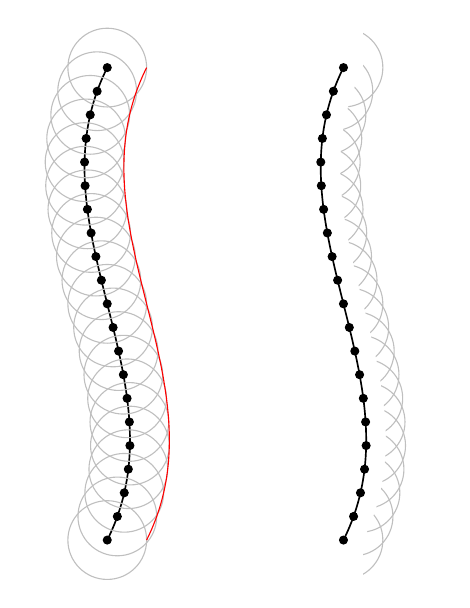
\begin{tikzpicture}
            \draw[semithick] (0, 0) .. controls (1, 2) and (-1, 4) .. (0, 6);
            \foreach \i in {0, 0.05, ..., 1.05} {
                \draw[draw=none] (0, 0) .. controls (1, 2) and (-1, 4) .. (0, 6) coordinate[pos=\i] (A) {};
                \draw[fill=black] (A) circle[radius=0.05cm];
                \draw[lightgray] (A) circle[radius=0.5cm];
            }
            \draw[red] (0.5, 0) .. controls (1.5, 2) and (-0.5, 4) .. (0.5, 6);
            
            \begin{scope}[xshift=3cm]
                \draw[semithick] (0, 0) .. controls (1, 2) and (-1, 4) .. (0, 6);
                \foreach \i in {0, 0.05, ..., 1.05} {
                    \draw[draw=none] (0, 0) .. controls (1, 2) and (-1, 4) .. (0, 6) coordinate[pos=\i] (A) {};
                    \draw[fill=black] (A) circle[radius=0.05cm];
                    \begin{scope}
                        \clip (0.25, -0.5) -- (0.25, 0) .. controls (1.25, 2) and (-0.75, 4) .. (0.25, 6) -- (0.25, 6.5) -- (1, 6.5) -- (1, -0.5) -- cycle;
                        \draw[lightgray] (A) circle[radius=0.5cm];
                    \end{scope}
                }
            \end{scope}
        \end{tikzpicture}
        \caption{Many points along a wavefront emit wavelets which form a new wavefront.}
        \label{fig:huygens principle}
    \end{figure}
    This can be seen in figure~\ref{fig:huygens principle}.
    What isn't clear is why we only consider wavelets propagating in the forward direction.
    The reason for this will be given later when we have discussed superposition and interference.
    
    \subsection{Colour}
    As human beings we give particular attention to the visible part of the spectrum because, well, we can see it.
    The physics isn't fundamentally different for the rest of the spectrum but it is worth spending some time considering the visible spectrum and how we see light.
    
    There are two types of colour.
    There are \define{pure}/\define{spectral}/\define{chromatic} colours such as red, blue, green, yellow, etc.\@ which are formed of a single wavelength and there are colours, such as purple or brown, which are a mixture of other colours.
    The pure colours are the ones we see when we pass light through a prism and split it up into a rainbow.
    
    \tikzexternaldisable
    \begin{table}[ht]
        \centering
        \definecolor{wavelengthViolet}{rgb}{0.356, 0, 0.75}
        \definecolor{wavelengthBlue}{rgb}{0.213, 0, 1}
        \definecolor{wavelengthGreenBlue}{rgb}{0, 0.622, 0.935}
        \definecolor{wavelengthBlueGreen}{rgb}{0, 0.898, 0.804}
        \definecolor{wavelengthGreen}{rgb}{0, 1, 0}
        \definecolor{wavelengthYellowGreen}{rgb}{0.93, 1, 0}
        \definecolor{wavelengthYellow}{rgb}{1, 0.725, 0}
        \definecolor{wavelengthOrange}{rgb}{1, 0.499, 0}
        \definecolor{wavelengthRed}{rgb}{0.818, 0, 0}
        \definecolor{wavelengthMagenta}{rgb}{1, 0, 1}
        \definecolor{wavelengthCyan}{rgb}{0, 1, 1}
        \begin{tabular}{cllll}\hline
            Wavelength (\si{\nano\metre}) & Colour & & & Complementary Colour\\\hline
            400--435 & Violet & \tikz{\fill[fill=wavelengthViolet] (0, 0) rectangle (0.25, 0.25);} & \tikz{\fill[fill=wavelengthYellowGreen] (0, 0) rectangle (0.25, 0.25);} & Yellow-Green\\
            435--480 & Blue & \tikz{\fill[fill=wavelengthBlue] (0, 0) rectangle (0.25, 0.25);} & \tikz{\fill[fill=wavelengthYellow] (0, 0) rectangle (0.25, 0.25);} & Yellow\\
            480--490 & Green-Blue & \tikz{\fill[fill=wavelengthGreenBlue] (0, 0) rectangle (0.25, 0.25);} & \tikz{\fill[fill=wavelengthOrange] (0, 0) rectangle (0.25, 0.25);} & Orange\\
            490--500 & Blue-Green & \tikz{\fill[fill=wavelengthBlueGreen] (0, 0) rectangle (0.25, 0.25);} & \tikz{\fill[fill=wavelengthRed] (0, 0) rectangle (0.25, 0.25);} & Red\\
            500--560 & Green & \tikz{\fill[fill=wavelengthGreen] (0, 0) rectangle (0.25, 0.25);} & \tikz{\fill[fill=wavelengthMagenta] (0, 0) rectangle (0.25, 0.25);} & Magenta\\
            560--580 & Yellow-Green & \tikz{\fill[fill=wavelengthYellowGreen] (0, 0) rectangle (0.25, 0.25);} & \tikz{\fill[fill=wavelengthViolet] (0, 0) rectangle (0.25, 0.25);} & Violet\\
            580--595 & Yellow & \tikz{\fill[fill=wavelengthYellow] (0, 0) rectangle (0.25, 0.25);} & \tikz{\fill[fill=wavelengthBlue] (0, 0) rectangle (0.25, 0.25);} & Blue\\
            595--605 & Orange & \tikz{\fill[fill=wavelengthOrange] (0, 0) rectangle (0.25, 0.25);} & \tikz{\fill[fill=wavelengthGreenBlue] (0, 0) rectangle (0.25, 0.25);} & Green-Blue\\
            605--700 & Red & \tikz{\fill[fill=wavelengthRed] (0, 0) rectangle (0.25, 0.25);} & \tikz{\fill[fill=wavelengthCyan] (0, 0) rectangle (0.25, 0.25);} & Cyan\\\hline
        \end{tabular}
    \end{table}
    \tikzexternalenable
    
    While many colours exist as a pure, single wavelength this is not how humans perceive colour.
    The human eye has three types of cones which are cells that can detect light.
    Each type preferentially detects light at one of three different wavelengths corresponding to red, green, and blue light.
    The brain then interprets both which cones are activated and also how much they are activated and combines this information to give us colour vision.
    For example if the red and green cones are activated a lot and the blue cones aren't activated at all then we see yellow:
    \tikzexternaldisable
    \definecolor{r}{rgb}{1,0,0}
    \definecolor{g}{rgb}{0,1,0}
    \definecolor{rg}{rgb}{1,1,0}
    \[\tikz{\fill[fill=r] (0, 0) rectangle (0.25, 0.25);} + \tikz{\fill[fill=g] (0, 0) rectangle (0.25, 0.25);} = \tikz{\fill[fill=rg] (0, 0) rectangle (0.25, 0.25);}.\]
    \tikzexternalenable
    If instead red is activated a lot and blue is activated about half as much then we see a sort of pink-purple colour:
    \tikzexternaldisable
    \definecolor{b}{rgb}{0,0,0.5}
    \definecolor{rb}{rgb}{1,0,0.5}
    \[\tikz{\fill[fill=r] (0, 0) rectangle (0.25, 0.25);} + \tikz{\fill[fill=b] (0, 0) rectangle (0.25, 0.25);} = \tikz{\fill[fill=rb] (0, 0) rectangle (0.25, 0.25);}.\]
    \tikzexternalenable
    We use this to produce colour in screens.
    Each pixel of a screen actually produces red, green, and blue, colour (RGB) in varying amounts which combine to give the colours we see.
    The standard way for this to happen is for the amount of each colour to be given by an 8 bit number which allows for values from 0 to 255.
    So for three different colours there are \(256^3 = 2^{8^3} = 2^{24} = 16777216\) different combinations that can be shown.
    This is just one of many ways of telling a computer what colour to show, an equivalent way uses hexadecimal instead and each colour is a six digit hexadecimal number ranging from \(\mathrm{\#000000} = 0\) for none of any colour (black) to \(\mathrm{\# FFFFFF} = 16777215\) for all of each colour (white).
    This isn't really that different as we can split the hexadecimal number into three two digit hexadecimal numbers each of which can be translated into binary to give the same three number RGB colour definition.
    
    Another aspect that needs to be considered is that the cones don't all only activate at a single wavelength but at a range of wavelengths and these ranges all overlap to some extent so light of a single wavelength can stimulate more than one type of cone at once which is how we see pure colours that aren't red, green, or blue.
    
    There are many mechanisms by which an object that doesn't produce its own light can become coloured in white light.
    We will discuss two right now.
    The simplest is colour by absorption.
    For example \ce{Cu^{2+}} absorbs most light except blue-green light and so when we see something with lots of \ce{Cu^{2+}} ions most of the light that bounces off of it is blue-green so this is the colour we see the object.
    The second mechanism is more complicated and involves scattering light at different wave lengths different amounts in such a way that most colours are scattered away before reaching us.
    This is the mechanism by which the sky appears blue.
    Scattering in the atmosphere scatters higher frequencies the most the light leaving the sun is pretty much white and so if you look directly at the sun\footnote{don't do this} you will see white light.
    Looking near the sun you see red/yellow light that has been scattered only a little bit.
    Looking far from the sun you see blue light which has been scattered far from the sun.
    The only reason that the sky isn't purple (as this light is the most scattered) is because the sun doesn't actually produce much purple light.
    
    \part[Light at Boundaries -- Reflection and Refraction]{Light at Boundaries\\{\LARGE Reflection and Refraction}}
    \section{Laws of Reflection and Refraction}
    We are mostly interested in this part in light incident on a sudden boundary between materials with different refractive indices.
    We will assume that the boundaries are smooth (on the scale of the wavelength).
    Recall that the angle of incidence is defined as the angle the incoming light makes to the surface normal pointing out of the surface.
    Similarly the angle of reflection is the angle that the reflected light makes to the same normal and the angle of transmission is the angle the transmitted light makes to the surface normal pointing into the surface.
    
    \subsection{Snell's Law}
    We have seen already in section~\ref{sec:snell's law fermat's principle} a derivation of Snell's law which depended on Fermat's principle---that light minimises the time taken to travel between points.
    We can also derive the same law with a full treatment of the equations for electromagnetic waves.
    
    Consider a boundary between two media with surface normal \(\vv{e}\).
    Incident on this surface is light with wave vector \(\vv{k_i}\).
    We would expect in general that there will be both reflection and transmission.
    The wave vector, \(\vv{k_i}\), and the surface normal, \(\vv{e}\), define a plane, called the plane of incidence.
    For a smooth surface all reflected and transmitted light will still be in this plane.
    The equation of the incoming light is
    \[\vv{E_i} = \vv{E_{0i}} \cos(\vv{k_i} \cdot \vv{r} - \omega t)\]
    where \(\vv{E_{0i}}\) is the amplitude and \(\omega\) is the frequency of the light.
    The energy of light is proportional to \(\omega\) and so to conserve energy the reflected and transmitted light must have the same frequency as the incident light.
    This means that we can express the electric field of the reflected light as
    \[\vv{E_r} = \vv{E_{0r}} \cos(\vv{k_r} \cdot \vv{r} 0 \omega t - \Phi_r)\]
    where \(\Phi_r\) is some phase difference to be calculated.
    Similarly the transmitted field is given by
    \[\vv{E_t} = \vv{E_{0t}} \cos(\vv{k_t} \cdot \vv{r} - \omega t - \Phi_t).\]
    We will start by computing the direction of propagation and the time dependence which means finding the wave vectors and phase factors.
    Later we will work out how the amplitudes are related.
    
    In order to satisfy Maxwell's equations the components of \(\vv{E}\) and \(\vv{H}\) which are parallel to the interface must be continuous across the boundary.
    We choose to define our coordinate system such that \(\ve{z} = \vv{e}\) is the surface normal and \(\ve{x}\) lies in the plane of incidence.
    This means that none of the wave vectors have a component in the \(\ve{y}\) direction.
    For example the incoming wave vector can be written as \(\vv{k_i} = k_i\sin\vartheta_i\ve{x} - k_i\cos\vartheta_i\ve{z}\) where \(\vartheta_i\) is the angle of incidence defined as the angle \(\vv{k_i}\) makes to \(\ve{z}\).
    In order for the boundary conditions at the surface to hold at all times we must have that
    \[\vv{k_i}\cdot\vv{r} = \vv{k_r}\cdot\vv{r} - \Phi_{r} = \vv{k_t}\cdot\vv{r} - \Phi_t.\]
    Rearranging this we have that \((\vv{k_i} - \vv{k_r})\cdot\vv{r} = \Phi_r\).
    Compare this to the equation \(\vv{n}\cdot\vv{r} = a\) for some constant \(a\) which defines a plane with surface normal \(\vv{n}\).
    Since we are considering the fields at the boundary we have already restricted \(\vv{r}\) to be on the surface which means that the surface normal to the plane we are defining with this equation is \(\vv{k_i} - \vv{k_r}\).
    This means that \(\vv{k_i} - \vv{k_r} \propto \ve{z}\).
    This means that the \(x\) and \(y\) components must cancel so \(k_{ix} = k_{rx}\) and \(k_{iy} = k_{ry}\).
    We know that \(k_{iy} = 0\) from how we define the coordinate system so \(k_{ry} = 0\) also.
    Simple geometry shows that \(k_{ix} = k_i\sin\vartheta_i\) and \(k_{rx} = k_i\sin\vartheta_r\).
    Converting wave numbers to wavelengths we have
    \[\frac{2\pi}{\lambda_i} \sin\vartheta_i = \frac{2\pi}{\lambda_r}\sin\vartheta_r.\]
    Since \(\omega\) is the same in all cases and the incident and reflected wave are in the same medium so they must have the same wavelength, \(\lambda_i = \lambda_r\).
    This means that \(\vartheta_i = \vartheta_r\).
    This is called the \define{law of reflection}, that the incident and reflected angle are the same.
    Similar calculations give imply that
    \[k_i\sin\vartheta_i = k_t\sin\vartheta_t.\]
    Introducing the refractive indices which relate the wavelengths by \(n_i\lambda_i = n_t\lambda_t\) and cancelling common factors we get
    \[n_i\sin\vartheta_i = n_t\sin\vartheta_t.\]
    This is \define{Snell's law} again.
    
    \subsection{Total Internal Reflection}
    Consider a light incident on a boundary from a high refractive index to a low refractive index.
    From Snell's law we have
    \[\sin\vartheta_l = \frac{n_h}{n_l}\sin\vartheta_h\]
    where subscript \(l\) and \(h\) refer to quantities measured in the low and high refractive index media respectively.
    We expect that \(\vartheta_l > \vartheta_h\) and this is indeed the case up to some critical angle \(\vartheta_l = \criticalAngle\) at which point \(\sin\criticalAngle = 1\) and instead of being transmitted the incident light is reflected.
    The critical angle is simply given by
    \[\criticalAngle = \arcsin\left( \frac{n_l}{n_h} \right).\]
    We call this total internal reflection.
    This is the mechanism by which an optical fibre works, light is shone in at one end at such an angle that it always meets the outside (or in real use the outer layer of cladding) above the critical angle and is reflected back inside the fibre.
    
    Another use of this effect is measuring the refractive index of a material as it is easy to measure the critical angle with \(n_l\) being some known value, such as air so \(n_l \approx 1\).
    For example if we measure the critical angle of a glass block to be \(42^\circ\) then
    \[n_h = \frac{1}{\sin\vartheta} = \frac{1}{\sin 42^\circ} = 1.5\]
    which is a fairly standard refractive index for glass.
    
    \subsection{Dispersion}
    We know that the refractive index of a material differs with frequency.
    This means that different colours of light are refracted a different amount.
    This is the mechanism by which a prism is able to split white light into a rainbow.
    This effect also allows us to see which wavelengths \emph{aren't} present in light which gives us the absorption spectra of a source which we can tell us about the chemical composition of the source.
    
    The dispersion of a material is simply how much \(n\) varies with \(\lambda\).
    For example diamond is highly dispersive and can also be cut to have lots of flat planes.
    If these planes are cut at the correct angles then we also get lots of total internal reflection.
    These two effects combine to mean that most light that enters a diamond leaves out the front and also is separated slightly into different colours.
    This makes diamonds very nice to look at.
    In part this is due to the high refractive index of diamond, \(n = 2.419\), which ensures a low critical angle.
    Thus light can only leave at certain angles which gives diamond its characteristic sparkle.
    
    \subsection{Lenses}
    Lenses rely on the refraction of light to bend incident light such that it converges on a focal point at focal length \(f\).
    Simple lenses can be described by three numbers.
    The refractive index of the material it is made from and the radius of curvature of the two faces.
    The radius of curvature is the radius of a sphere which has the same curvature as the lens and it is a signed number with the sign being positive if the edges of the lens bend in the positive direction along the optical axis and negative if the centre of the lens bulges along the optical axis (see figure~\ref{fig:radii of curvature}).
    We say that lens is thin if its thickness, \(\Delta\), satisfies \(\Delta < \abs{R_1}\) and \(\Delta < \abs{R_2}\) where \(R_i\) are the radii of curvature.
    For a thin lens the focal distance is given by the \define{lens makers formula}:
    \[\frac{1}{f} = (n - 1) \left[ \frac{1}{R_1} - \frac{1}{R_2} \right]\]
    One problem is that since \(n\) varies with wavelength the focal point also varies with wavelength.
    This is called a chromatic aberration.
    \begin{figure}[htb]
        \centering
        \tikzsetnextfilename{lens-radii-curvature}
        \begin{tikzpicture}
            \begin{scope}
                \clip (0, 0) -- (45:5) -- (-45:5) -- cycle;
                \draw[ultra thick] (0, 0) circle[radius=3cm];
            \end{scope}
            \begin{scope}
                \clip (0, 0) -- (135:5) -- (-135:5) -- cycle;
                \draw[ultra thick] (0, 0) circle[radius=3cm];
            \end{scope}
            \draw[very thick, ->, >=latex] (0, 0) -- (30:3) node[midway, above] {\(R_2\)};
            \draw[very thick, ->, >=latex] (0, 0) -- (150:3) node[midway, above] {\(R_1\)};
            \draw[->, >=latex] (-5, 0) -- (5, 0) node[right] {\(z\)};
        \end{tikzpicture}
        \caption{Two possible faces of a lens with the same absolute radius of curvature but different signs, \(R_1 > 1\) and \(R_2 < 1\).}
        \label{fig:radii of curvature}
    \end{figure}

    \subsection{Optical Illusions}
    \subsubsection{Snell's Window}
    Suppose that you are underwater and you look up.
    If the surface is sufficiently flat you will see only be able to see out of the water in some circle (see figure~\ref{fig:snell's window irl}).
    Outside of this circle the angle is such that instead total internal reflection would occur and you would see back down into the water.
    This is best demonstrated by looking at figure~\ref{fig:snell's window}.
    \begin{figure}[htbp!]
        \centering
        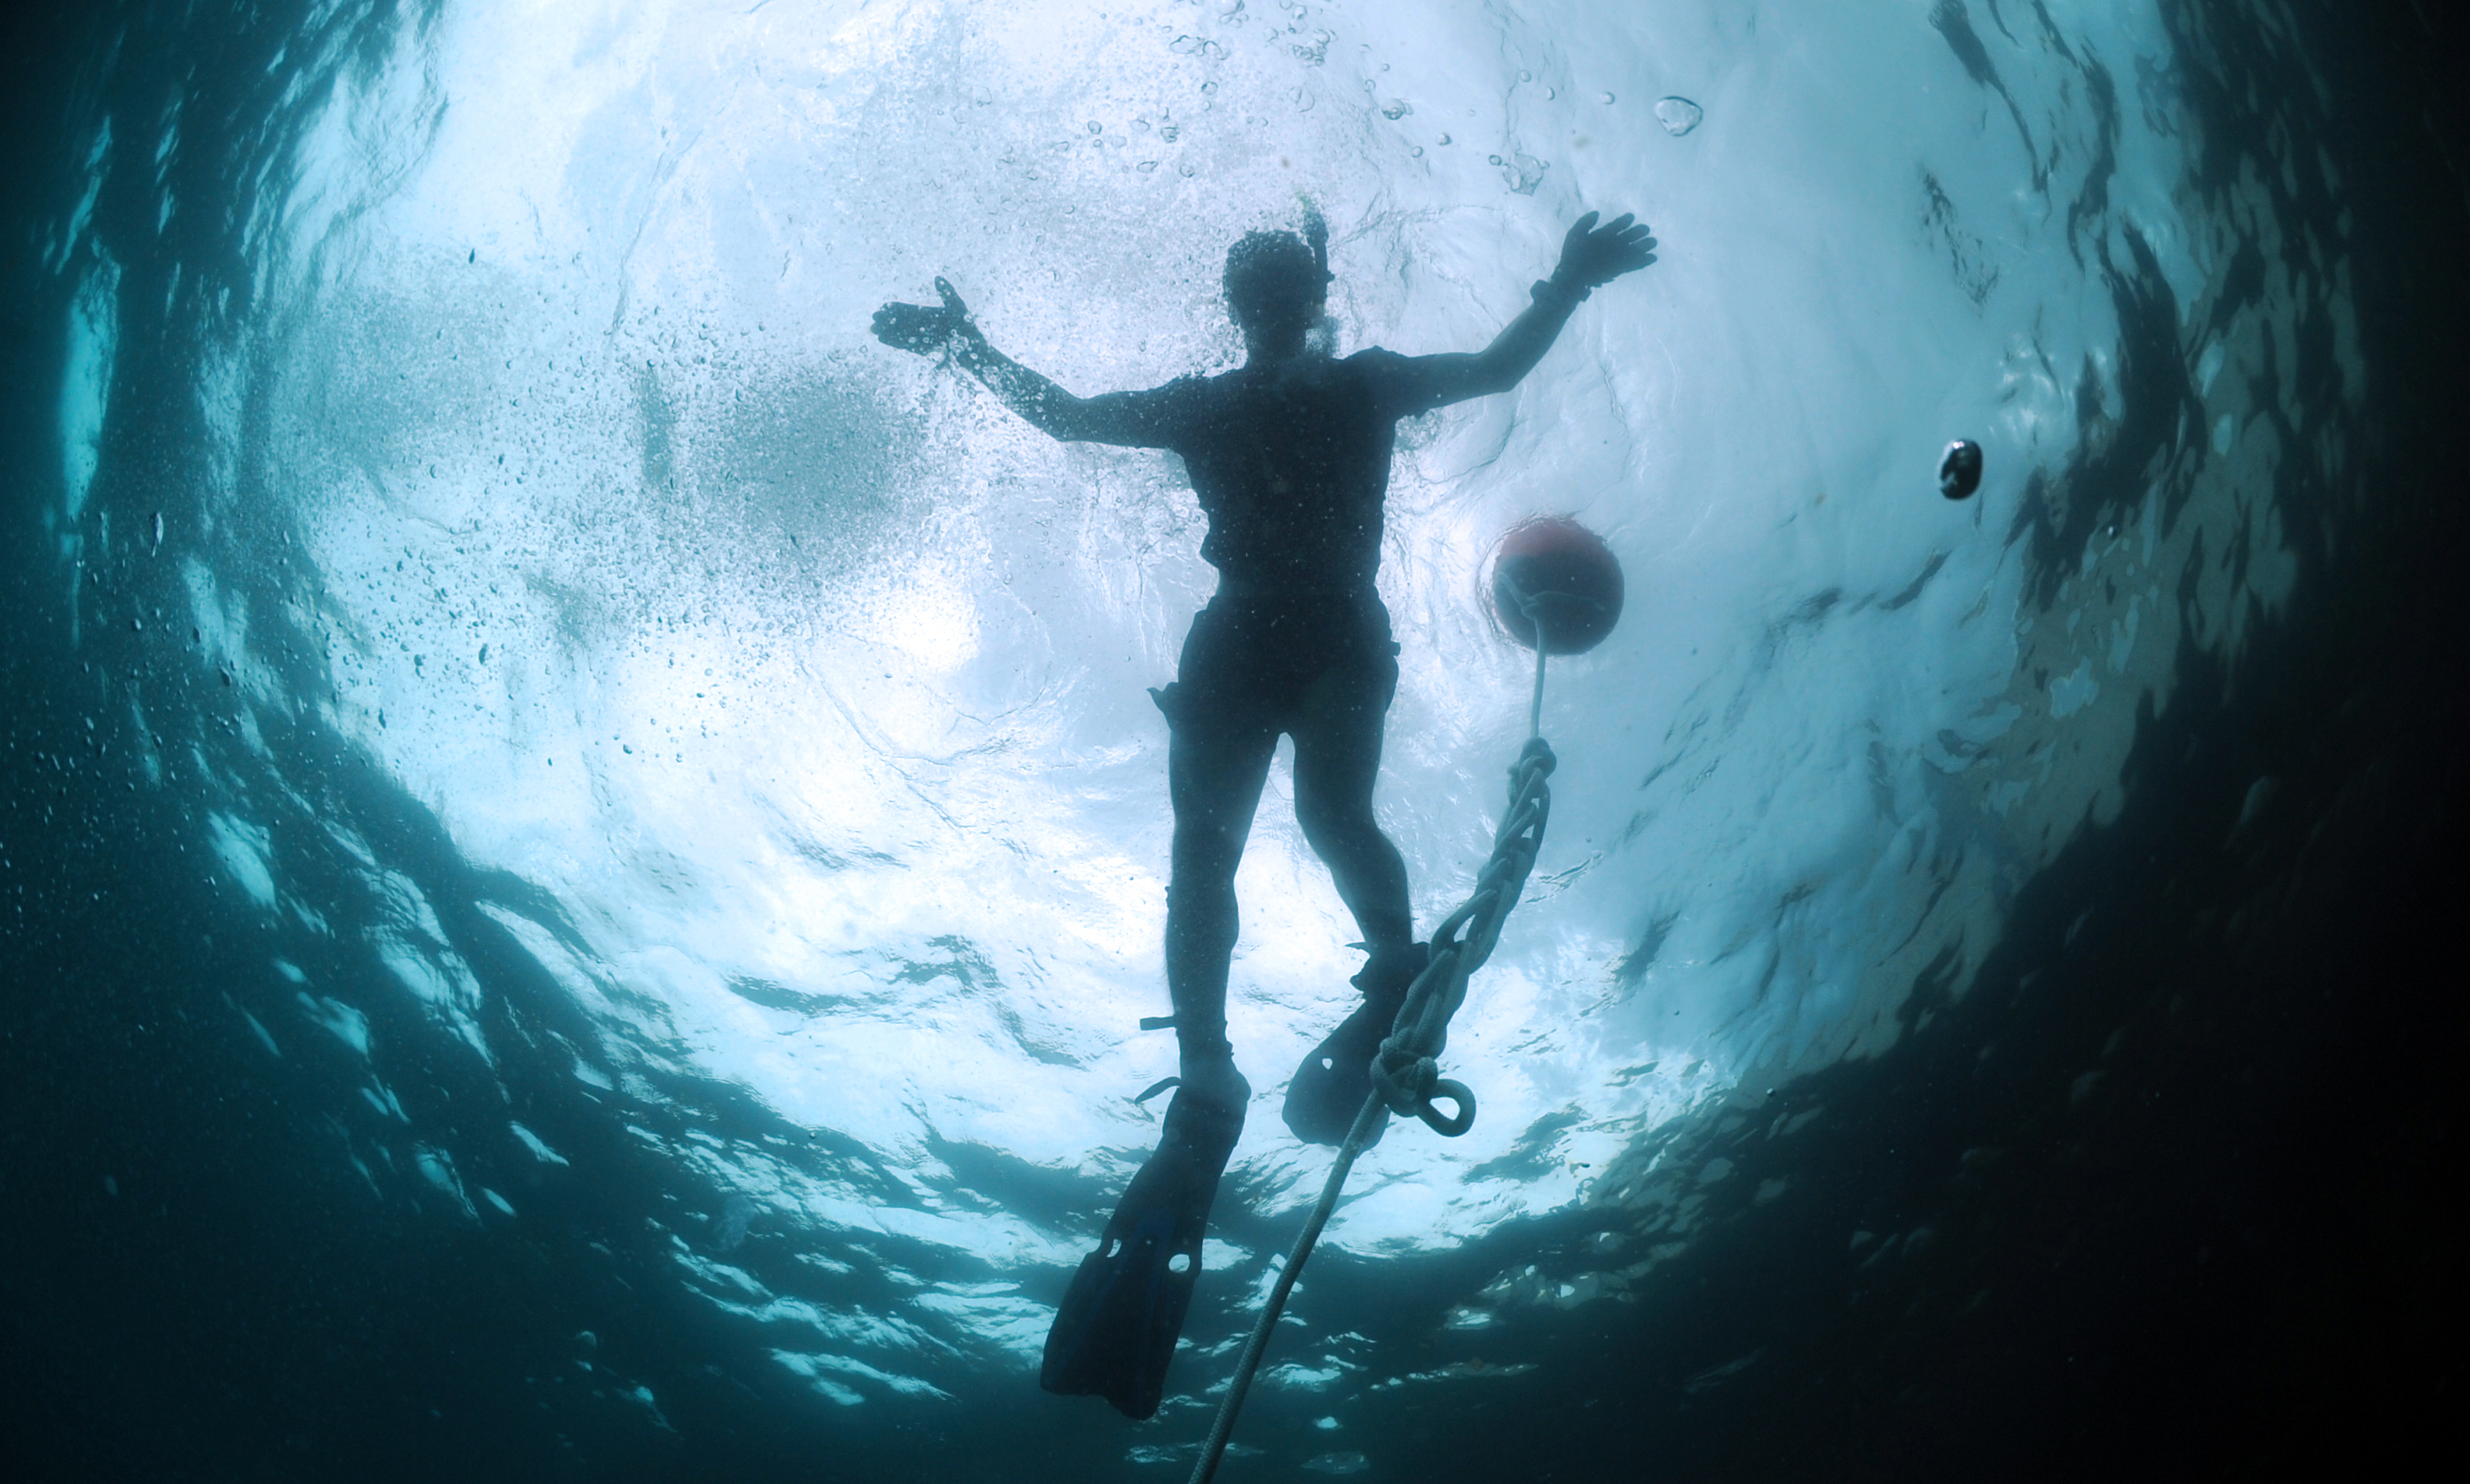
\includegraphics[scale=0.4]{snellswindow.jpg}
        \caption{Snell's window in real life. Image credit: \url{https://commons.wikimedia.org/wiki/File:US_Navy_110607-N-XD935-191_Navy_Diver_2nd_Class_Ryan_Arnold,_assigned_to_Mobile_Diving_and_Salvage_Unit_2,_snorkels_on_the_surface_to_monitor_multi.jpg} accessed on 27/04/2021.}
        \label{fig:snell's window irl}
    \end{figure}
    \begin{figure}[htbp!]
        \centering
        \tikzsetnextfilename{snells-window}
        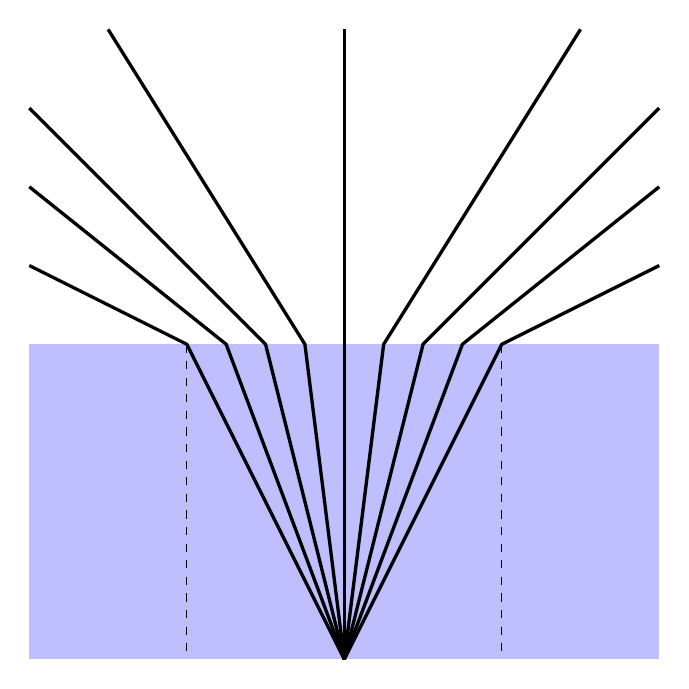
\begin{tikzpicture}
            \fill[blue!50, opacity=0.5] (-4, -4) rectangle (4, 0);
            \draw[very thick] (0, -4) -- (-2, 0) -- (-4, 1);
            \draw[very thick] (0, -4) -- (2, 0) -- (4, 1);
            \draw[very thick] (0, -4) -- (-1.5, 0) -- (-4, 2);
            \draw[very thick] (0, -4) -- (1.5, 0) -- (4, 2);
            \draw[very thick] (0, -4) -- (-1, 0) -- (-4, 3);
            \draw[very thick] (0, -4) -- (1, 0) -- (4, 3);
            \draw[very thick] (0, -4) -- (-0.5, 0) -- (-3, 4);
            \draw[very thick] (0, -4) -- (0.5, 0) -- (3, 4);
            \draw[very thick] (0, -4) -- (0, 0) -- (0, 4);
            \draw[dashed] (-2, 0) -- (-2, -4);
            \draw[dashed] (2, 0) -- (2, -4);
        \end{tikzpicture}
        \caption{Looking up from underwater you only see out of a circle, known as Snell's window. Outside of this circle total internal reflection occurs and you see back down into the water.}
        \label{fig:snell's window}
    \end{figure}
    
    \subsubsection{Mirages}
    The refractive index of air depends on its density and hence on the temperature of the air.
    This means that on a hot day the refractive index changes a non-negligible amount between the ground and a few metres up as the air is hotter higher up.
    Imagine light coming off the top of a tree towards the ground.
    We can consider each step along the path the light takes to be going through a boundary with two different refractive indexes.
    If the conditions are just right this can cause the light to refract slightly at each step until it is travelling upwards.
    If we see this light that came from the top of a tree but is travelling upwards towards us our brains are unable to comprehend the process that has actually taken place and instead assume that the light has reflected off of something.
    Our monkey brains are also trained to see anything reflective as a source of water and therefore it is common for it to look like there is water on the ground even though there isn't.
    This is the mechanism behind heat hazes and mirages.
    
    \section{The Fresnel Equations}
    In the last section we discussed reflection and refraction with a focus on the angles that the rays make to the surface normals.
    We found that an incident ray is reflected at the same angle it is incident and that the transmitted ray will be at an angle satisfying Snell's law:
    \[n_i\sin\vartheta_i = n_t\sin\vartheta_t.\]
    To find this we solved for the wave vectors \(\vv{k_r}\) and \(\vv{k_t}\).
    We didn't however, find the amplitudes of the reflected and transmitted waves.
    This is what we will do in this section.
    To find the amplitudes we need to be slightly more cautious in our calculations and consider the direction the waves oscillate.
    There are two linearly independent directions that an incident wave can oscillate and all other cases are simply a superposition of these two cases:
    \begin{itemize}
        \item If \(\vv{E_{0i}}\) is perpendicular to the plane of incidence then we call the wave \define{transverse electric} or S-polarised\footnote{S for \textit{senkrecht}, German for perpendicular.}.
        \item If \(\vv{E_{0i}}\) is parallel to the plane of incidence then we call the wave \define{transverse magnetic} or P-polarised\footnote{P for \textit{parallel}, German for parallel.}.
    \end{itemize}
    We will treat these two cases separately.
    
    \subsection{S-Polarised Light}
    The boundary conditions for \(\vv{E}\) are that the components parallel to the boundary are continuous across the boundary.
    For S-polarised light the incoming amplitudes are perpendicular to the plane of incidence which necessarily makes them parallel to the boundary.
    Thus we must have at the boundary that
    \begin{equation}\label{eqn:continuity of electric field at boundary}
        E_{0i} + E_{0r} = E_{0t}.
    \end{equation}
    The boundary conditions are slightly more tricky for \(\vv{H}\).
    It is conventional to define \(\vv{k}\), \(\vv{E}\), and \(\vv{H}\) such that they form a right handed system.
    Considering an incoming wave being reflected the direction of \(\vv{k}\) is set by the direction of travel and the direction of \(\vv{E}\) is set by demanding S-polarised light.
    The result is that we have to choose to define the direction of \(\vv{H}\) to keep a right handed system as shown in figure~\ref{fig:S-polarised light}.
    \begin{figure}[ht]
        \centering
        \tikzsetnextfilename{reflection-transmission-amplitude-s-polarised}
        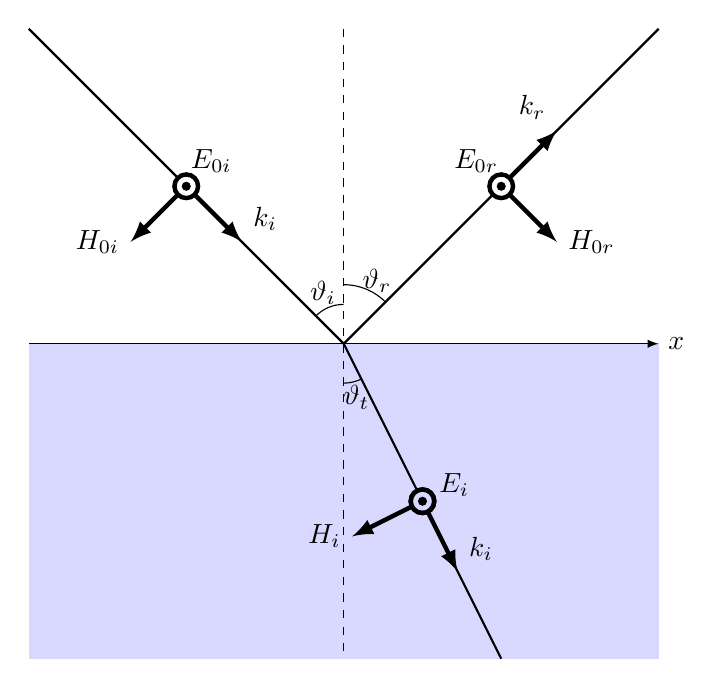
\begin{tikzpicture}
            \fill[blue!50, opacity=0.3] (-4, -4) rectangle (4, 0);
            \draw[thick] (-4, 4) -- (0, 0) -- (4, 4);
            \draw[thick] (0, 0) -- (2, -4);
            \draw[dashed] (0, 4) -- (0, -4);
            \draw[->, >=latex] (-4, 0) -- (4, 0) node[right] {\(x\)};
        
            \begin{scope}[xshift=-2cm, yshift=2cm]
                \draw[ultra thick, ->, >=latex] (0, 0) -- (-45:1) node[above right] {\(\vv{k_i}\)};
                \draw[ultra thick, ->, >=latex] (0, 0) -- (-135:1) node[left] {\(\vv{H_{0i}}\)};
                \draw[ultra thick, fill=white] (0, 0) circle[radius=0.15cm];
                \draw[fill=black] (0, 0) circle[radius=0.05cm];
                \node at (45:0.45) {\(\vv{E_{0i}}\)};
            \end{scope}
        
            \begin{scope}[xshift=2cm, yshift=2cm]
                \draw[ultra thick, ->, >=latex] (0, 0) -- (45:1) node[above left] {\(\vv{k_r}\)};
                \draw[ultra thick, ->, >=latex] (0, 0) -- (-45:1) node[right] {\(\vv{H_{0r}}\)};
                \draw[ultra thick, fill=white] (0, 0) circle[radius=0.15cm];
                \draw[fill=black] (0, 0) circle[radius=0.05cm];
                \node at (135:0.45) {\(\vv{E_{0r}}\)};
            \end{scope}
        
            \begin{scope}[xshift=1cm, yshift=-2cm]
                \draw[ultra thick, ->, >=latex] (0, 0) -- ({atan(1/2)-90}:1) node[above right] {\(\vv{k_i}\)};
                \draw[ultra thick, ->, >=latex] (0, 0) -- ({atan(1/2)+180}:1) node[left] {\(\vv{H_i}\)};
                \draw[ultra thick, fill=white] (0, 0) circle[radius=0.15cm];
                \draw[ultra thick, fill=blue!50, fill opacity=0.3] (0, 0) circle[radius=0.15cm];
                \draw[fill=black] (0, 0) circle[radius=0.05cm];
                \node at ({atan(1/2)}:0.45) {\(\vv{E_i}\)};
            \end{scope}
        
            \begin{scope}
                \clip (0, 0) -- (-4, 4) -- (0, 4) -- cycle;
                \draw (0, 0) circle[radius=0.5cm];
            \end{scope}
            \begin{scope}
                \clip (0, 0) -- (4, 4) -- (0, 4) -- cycle;
                \draw (0, 0) circle[radius=0.75cm];
            \end{scope}
            \begin{scope}
                \clip (0, 0) -- (2, -4) -- (0, -4) -- cycle;
                \draw (0, 0) circle[radius=0.5cm];
            \end{scope}
            \node at (112:0.7) {\(\vartheta_i\)};
            \node at (62:0.9) {\(\vartheta_r\)};
            \node at ({-90+atan(1/2)/2}:0.7) {\(\vartheta_t\)};
        \end{tikzpicture}
        \caption{S-polarised light reflection and transmission.}
        \label{fig:S-polarised light}
    \end{figure}
    In particular we have \(\vv{k}\times\vv{E} = v\vv{B}\).
    We can then show that the continuity equation for \(\vv{H}\) is
    \[H_{0i}\cos\vartheta_i - H_{0r}\cos\vartheta_r = H_{0t}\cos\vartheta_t.\]
    Writing \(H = B/\mu = E/(v\mu) = En/(c\mu)\) and \(\vartheta_r = \vartheta_i\) we have
    \begin{align*}
        \frac{B_{0i}}{\mu_i}\cos\vartheta_i - \frac{B_{0r}}{\mu_i}\cos\vartheta_i &= \frac{B_{0t}}{\mu_t}\cos\vartheta_t\\
        \frac{E_{0i}n_i}{c\mu_i}\cos\vartheta_i - \frac{E_{0r}n_i}{c\mu_i}\cos\vartheta_i &= \frac{E_{0t}n_t}{c\mu_t}\cos\vartheta_t\\
        (E_{0i} - E_{0r})\frac{n_i\cos\vartheta_i}{c\mu_i} = E_{0t}\frac{n_t\cos\vartheta_t}{c\mu_t} &= (E_{0i} + E_{0r})\frac{n_t\cos\vartheta_t}{c\mu_t}
    \end{align*}
    where in the last equality we have used the continuity equation for the electric field (equation~\ref{eqn:continuity of electric field at boundary}).
    Since we can link \(\vartheta_i\) and \(\vartheta_t\) by Snell's law and we can measure the material properties \(\mu_i\), \(\mu_t\), \(n_i\), and \(n_t\) this equation gives us a relationship between the amplitudes of the incident magnetic field, \(E_{0i}\), and the reflected field, \(E_{0r}\).
    
    We further assume that the magnetic field is not that strong and so it is a reasonable approximation to assume that \(\mu_i = \mu_t = \mu_0\).
    We define the \define{Fresnel reflection coefficient} as the ratio \(E_{0r}/E_{0i}\) which for S-polarised light we find to be
    \[\fresnelCoeff{r}{S} = \frac{E_{0r}}{E_{0i}} = \frac{n_i\cos\vartheta_{i} - n_t\cos\vartheta_{t}}{n_i\cos\vartheta_i + n_t\cos\vartheta_t}.\]
    We can use the same equations and instead eliminate \(E_{0r}\) leaving us with a relationship between \(E_{0t}\) and \(E_{0i}\).
    Similarly we can then define the \define{Fresnel trnasmission coefficeint} for S-polarised light:
    \[\fresnelCoeff{t}{S} = \frac{E_{0t}}{E_{0i}} = \frac{2n_{i}\cos\vartheta_{i}}{n_i\cos\vartheta_{i} + n_t\cos\vartheta_{t}}.\]
    
    \subsection{P-Polarised Light}
    The case of P-polarised light is very similar with slightly different boundary conditions.
    This time the \(\vv{H}\) continuity equation is simple:
    \[H_{0i} + H_{0r} = H_{0t}\]
    and the \(\vv{E}\) continuity equations are the more complicated
    \[E_{0i}\cos\vartheta_i - E_{0r}\cos\vartheta_i = E_{0t}\cos\vartheta_t.\]
    We can similarly define \define{Fresnel coefficients} for reflection and transmission of P-polarised light:
    \begin{align*}
        \fresnelCoeff{r}{P} &= \frac{E_{0r}}{E_{0i}} = \frac{n_t\cos\vartheta_i - n_i\cos\vartheta_t}{n_i\cos\vartheta_t + n_t\cos\vartheta_i},\\
        \fresnelCoeff{t}{P} &= \frac{E_{0t}}{E_{0i}} = \frac{2n_i\cos\vartheta_i}{n_i\cos\vartheta_t + n_t\cos\vartheta_i}.\\
    \end{align*}
    \begin{figure}[ht]
        \centering
        \tikzsetnextfilename{reflection-transmission-amplitude-p-polarised}
        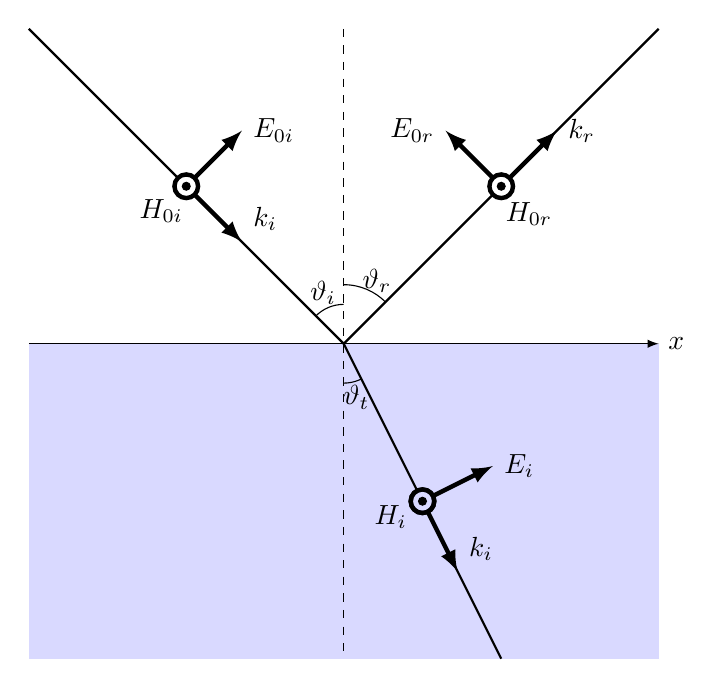
\begin{tikzpicture}
            \fill[blue!50, opacity=0.3] (-4, -4) rectangle (4, 0);
            \draw[thick] (-4, 4) -- (0, 0) -- (4, 4);
            \draw[thick] (0, 0) -- (2, -4);
            \draw[dashed] (0, 4) -- (0, -4);
            \draw[->, >=latex] (-4, 0) -- (4, 0) node[right] {\(x\)};
            
            \begin{scope}[xshift=-2cm, yshift=2cm]
                \draw[ultra thick, ->, >=latex] (0, 0) -- (-45:1) node[above right] {\(\vv{k_i}\)};
                \draw[ultra thick, ->, >=latex] (0, 0) -- (45:1) node[right] {\(\vv{E_{0i}}\)};
                \draw[ultra thick, fill=white] (0, 0) circle[radius=0.15cm];
                \draw[fill=black] (0, 0) circle[radius=0.05cm];
                \node at (-135:0.45) {\(\vv{H_{0i}}\)};
            \end{scope}
            
            \begin{scope}[xshift=2cm, yshift=2cm]
                \draw[ultra thick, ->, >=latex] (0, 0) -- (45:1) node[right] {\(\vv{k_r}\)};
                \draw[ultra thick, ->, >=latex] (0, 0) -- (135:1) node[left] {\(\vv{E_{0r}}\)};
                \draw[ultra thick, fill=white] (0, 0) circle[radius=0.15cm];
                \draw[fill=black] (0, 0) circle[radius=0.05cm];
                \node at (-45:0.5) {\(\vv{H_{0r}}\)};
            \end{scope}
            
            \begin{scope}[xshift=1cm, yshift=-2cm]
                \draw[ultra thick, ->, >=latex] (0, 0) -- ({atan(1/2)-90}:1) node[above right] {\(\vv{k_i}\)};
                \draw[ultra thick, ->, >=latex] (0, 0) -- ({atan(1/2)}:1) node[right] {\(\vv{E_i}\)};
                \draw[ultra thick, fill=white] (0, 0) circle[radius=0.15cm];
                \draw[ultra thick, fill=blue!50, fill opacity=0.3] (0, 0) circle[radius=0.15cm];
                \draw[fill=black] (0, 0) circle[radius=0.05cm];
                \node at ({180+atan(1/2)}:0.45) {\(\vv{H_i}\)};
            \end{scope}
            
            \begin{scope}
                \clip (0, 0) -- (-4, 4) -- (0, 4) -- cycle;
                \draw (0, 0) circle[radius=0.5cm];
            \end{scope}
            \begin{scope}
                \clip (0, 0) -- (4, 4) -- (0, 4) -- cycle;
                \draw (0, 0) circle[radius=0.75cm];
            \end{scope}
            \begin{scope}
                \clip (0, 0) -- (2, -4) -- (0, -4) -- cycle;
                \draw (0, 0) circle[radius=0.5cm];
            \end{scope}
            \node at (112:0.7) {\(\vartheta_i\)};
            \node at (62:0.9) {\(\vartheta_r\)};
            \node at ({-90+atan(1/2)/2}:0.7) {\(\vartheta_t\)};
        \end{tikzpicture}
        \caption{P-polarised light reflection and transmission.}
    \end{figure}

    \subsection{Fresnel Coefficients With Incidence Angle}
    Consider light incident on glass (\(n = 1.5\)) travelling from air (\(n = 1\)).
    For normal, or almost normal incidence (\(\vartheta_i \approx 0\)) we see that for both S and P-polarised light we have \(\abs{t} \gg \abs{r}\).
    Comparing this to our daily experiences this makes sense as we are used to light passing straight through glass.
    For grazing incidence (\(\vartheta_i \approx \pi/2\)) we see that \(\abs{t} \approx 0\) and \(\abs{r} \approx 1\).
    Again this should be familiar that glass viewed at a large incidence angle is almost entirely reflective.
    
    For all angles of incidence it turns out that \(\fresnelCoeff{r}{S} < 0\).
    This corresponds to the incident and reflected \(\vv{E}\) fields being antiparallel.
    That is S-polarised light undergoes a phase shift of \(\pi\) when reflecting off of a higher refractive index medium.
    
    For P-polarised light at some point \(\fresnelCoeff{r}{P}\) becomes zero.
    The angle, \(\brewstersAngle\), at which this occurs is called \define{Brewster's angle}.
    At this angle there is no reflection.
    
    The transmission coefficients are similar (but not identical, note the refractive indices in the denominator swap) for both S and P-polarised light.
    It is mostly in reflection where the polarisation is important.
    
    Now consider the opposite case of light incident on a glass-air boundary from within the glass.
    For near normal incidence almost all light is transmitted.
    For P-polarised light there is an angle at which no light is reflected.
    This is sometimes referred to as the \define{internal Brewster's angle}.
    Note that this angle is \emph{not} the same angle as for the air-glass boundary.
    
    There is no phase shift for reflection of S-polarised light (as opposed to the \(\pi\) phase shift for the air-glass case).
    
    Above some critical angle, \(\criticalAngle\), both \(\fresnelCoeff{r}{S}\) and \(\fresnelCoeff{r}{P}\) are 1 and \(\fresnelCoeff{t}{S}\) and \(\fresnelCoeff{t}{P}\) are 0.
    This corresponds to total internal reflection.
    
    Perhaps the seemingly weirdest thing is that \(t > 1\) which means that, even if some light is reflected, the incident electric field has a smaller amplitude than the transmitted electric field.
    We will see in the next section why this must be the case.
    
    \subsection{Energy Flow}
    The amplitude of the transmitted field being greater than the amplitude of the incident field initially seems to violate energy conservation.
    As is often the case in electromagnetism this is because energy scales with the \emph{square} of the amplitude.
    For an oscillating field the most useful quantity is the intensity, \(I\), defined as the time average of the magnitude of the Poynting vector, \(\vv{S}\):
    \[I = \expected{S} = \frac{v\varepsilon}{2}E_0^2.\]
    Here \(v = c/n\) and we replace \(\varepsilon_0\) with \(\varepsilon\) when inside a medium.
    This gives the power density per unit area normal to the Poynting vector.
    
    Suppose we illuminate an area, \(A\), on a surface.
    To conserve energy we have to have the energy in per unit time be equal to the energy out per unit time.
    That is
    \[I_iA\cos\vartheta_i = I_rA\cos\vartheta_r + I_tA\cos\vartheta_t\]
    where \(I_i\), \(I_r\), and \(I_t\) are the intensities of the incident, reflected, and transmitted, field respectively.
    We can rearrange this and use the fact that \(\vartheta_i = \vartheta_r\) to get
    \[\frac{I_r}{I_i} + \frac{I_t}{I_i} \frac{\cos\vartheta_t}{\cos\vartheta_i} = 1.\]
    The first term gives the fraction of incident energy that is reflected and the second gives the fraction of incident energy that is transmitted.
    We call the first fraction the \define{reflectivity}:
    \[R = \frac{I_r}{I_i} = \frac{E_{0r}^2}{E_{0i}^2} = r^2.\]
    The second term we call the \define{transmissivity}:
    \[T = \frac{I_t}{I_i}\frac{\cos\vartheta_t}{\cos\vartheta_i} = \frac{E_{0t}^2}{E_{0i}^2} \frac{\mu_{ri}^2}{\mu_{rt}^2}\frac{n_t}{n_i}\frac{\cos\vartheta_t}{\cos\vartheta_i} \approx \frac{E_{0t}^2}{E_{0i}^2}\frac{n_t}{n_i}\frac{\cos\vartheta_t}{\cos\vartheta_i} = t^2\frac{n_t}{n_i}\frac{\cos\vartheta_t}{\cos\vartheta_i}.\]
    It can be shown that \(R + T = 1\) for all incident angle and this is the condition that energy is conserved.
    This explains why we can have \(t > 1\) so long as \(r\) is such that \(R +  T = 1\).
    
    At normal incidence for an air-glass boundary \SI{4}{\percent} of the light is reflected.
    For a single boundary this is negligible and we treat it as pure transmission.
    The issue arises with multiple boundaries, such as in a telescope or microscope, where there are multiple lenses and therefore the light we get out will be of significantly lower intensity than the light that we put in.
    The way that the unwanted reflected beams affect the image we get out is also non-trivial.
    
    So far in this section we have assumed that no energy is absorbed by the medium.
    If this isn't the case then the quantities \(r\), \(t\), \(n\), and \(\varepsilon\) become complex.
    We will see this more later.
    
    For a glass-air boundary above the critical angle \(R\) becomes 1 and \(T\) becomes 0.
    This is due to total internal reflection.
    
    \section{Consequences of the Fresnel Equations}
    \subsection{Total Internal Reflection}
    In the calculation of the Fresnel coefficients the transmission angle, \(\vartheta_t\), appears explicitly.
    The problem is that we can't define \(\vartheta_t\) for incidence angles greater than the critical angle.
    The way we solve this is by using Snell's law and trig identities:
    \[
        \left.
        \begin{array}{r}
        n_i\sin\vartheta_i = n_t\sin\vartheta_t \implies \sin\vartheta_t =  \frac{n_i}{n_t}\sin\vartheta_i\\
        \\
        \sin^2\vartheta_t + \cos^2\vartheta_t \implies \cos\vartheta_t = \sqrt{1 - \sin^2\vartheta_t}
        \end{array}
        \right\} \implies
        \cos\vartheta_t = \sqrt{1 - \frac{n_i^2}{n_t^2} \sin^2\vartheta_i}.
    \]
    Using this we can write the reflection coefficient as
    \[\fresnelCoeff{r}{S} = \frac{\cos\vartheta_i - \sqrt{n_t^2/n_i^2 - \sin^2\vartheta_i}}{\cos\vartheta_i + \sqrt{n_t^2/n_i^2 - \sin^2\vartheta_i}}.\]
    For cases where we have total internal reflection we have \(n_t/n_i < \sin\vartheta_i\) which means that the square roots result in complex numbers.
    We can generalise the reflectivity and transmissivity from the last section.
    In doing so we have to treat the S and P-polarised cases differently:
    \[\fresnelCoeff{R}{S} = \fresnelCoeff{r}{S}^*\fresnelCoeff{r}{S}, \qquad\text{and}\qquad \fresnelCoeff{R}{P} = \fresnelCoeff{r}{P}^*\fresnelCoeff{r}{P}.\]
    It can be shown that both reflectivities become 1 above the critical angle.
    
    When total internal reflection occurs the transmitted field has intensity 0.
    However in order for the correct continuity rules to apply we need to have a wave still.
    It can be shown that the if the transmitted wave vector is \(\vv{k_t}\) then the component parallel to the boundary is \(k_t\sin\vartheta_t\) which can be expressed as \(k_t(n_i/n_t)\sin\vartheta_i\) using Snell's law.
    The component perpendicular to the boundary can be expressed as
    \[k_t\cos\vartheta = k_t\sqrt{1 - \frac{n_i^2}{n_t^2}\sin^2\vartheta_i}.\]
    For total internal reflection we can write this as \(\pm i\beta\).
    This imaginary component to the wave vector corresponds to exponential decay of this component of the \(\vv{E}\) field.
    So for total internal reflection the transmitted ray decays to zero.
    These are called \define{evanescent} or \define{boundary waves}.
    If we make the low refractive index layer very thin then it is possible to get the transmitted wave out the other side before it decays to zero.
    This is called \define{frustrated total internal reflection}.
    
    \subsection{Metals and Plasmas}
    We saw something similar to evanescent waves when we considered electromagnetic fields incident on metal.
    We saw that the fields penetrate only a small amount, called the skin depth.
    
    Equation~\ref{eqn:epsilon r oscillator model} gives the relative permittivity derived from the oscillator model.
    If we allow for free electrons as well then we get instead
    \[\varepsilon_r = \varepsilon_r' + i\varepsilon_r'' = 1 + \frac{N\chargeElectron^2}{\varepsilon_0\massElectron} \left[ \frac{f_{\mathrm{e}}}{-\omega^2 - i\gamma_{\mathrm{e}}} + \sum_{j} \frac{f_j}{\omega_{0j}^2 - \omega^2 - i\gamma_j\omega} \right]\]
    The second term corresponds to the bound electrons summing over all relevant natural frequencies and the first term is the same but for unbound electrons so \(\omega_0 = 0\).
    The numerators, \(f_{\mathrm{e}}\) and \(f_j\) give the fraction of electrons that fall into each of these categories.
    
    The addition of the extra term changes the optical behaviour of the materials.
    For transparent dielectrics, such as glass, the natural frequency is \(\omega_0 \sim \SI{e16}{\radian.s^{-1}}\), which corresponds to the UV part of the spectrum.
    This means that visible light has \(\omega < \omega_0\) which we saw corresponds to the electron cloud oscillating \(\pi\) out of phase with \(\vv{E}\) and so the dipoles oscillate in phase with \(\vv{E}\).
    For free electrons the frequency of the driving force is above \(\omega_0\), even for visible light, which means that the oscillating electrons radiate wavelets that cancel the incident wave.
    
    Ignoring the bound electron's contribution and neglecting damping, \(\gamma_{\mathrm{e}} = 0\), the relative permittivity is given by
    \[\varepsilon_r = 1 - \frac{N\chargeElectron^2}{\varepsilon_0\massElectron\omega^2} = 1 - \frac{\omega_p^2}{\omega^2}\]
    where this equation defines \(\omega_p\), called the \define{plasma frequency}.
    For \(\omega < \omega_p\) we have \(\varepsilon_r < 0\) and hence the refractive index is imaginary, \(n = i\sqrt{\omega_p^2/\omega^2 - 1}\).
    The reflectivity at normal incidence can then be shown to be 1.
    If instead \(\omega > \omega_p\) then \(\varepsilon_r > 0\) and \(n = \sqrt{1 - \omega_p^2/\omega^2} \in\reals\).
    The reflectivity falls rapidly to zero as \(\omega\) increases.

    While these results only apply exactly for free electrons (a plasma) lots of metals can be reasonably approximated as a plasma of free electrons and some bound electrons and these results still approximately apply.
    This means that metals are transparent to light with \(\omega > \omega_p\).
    For most metals \(\omega_p\) is in the deep-UV part of the spectrum.
    
    The upper atmosphere is subject to intense solar radiation and is therefore highly ionised.
    Calculating \(\omega_p\) based on the charge density of the ionosphere we predict \(\omega_p\) to be in the \si{\mega\hertz} range meaning that lower frequency electromagnetic waves should be reflected back down to Earth.
    This is indeed the case and we use it to send radio messages from one place to another without direct line of site.
    
    \part{Superposition}
    \section{Superposition of Waves with the Same Wave Vector}
    So far we have only considered one wave at a time.
    If we want to consider more complicated phenomena such as multiple reflections or interference we need a solid mathematical understanding of what happens when two waves occupy the same region of space.
    We need superposition.
    
    The simplest case is two waves with the same wave vector and frequency.
    These waves differ only in their amplitude, \(E_{0i}\), and phase, \(\Phi_{i}\).
    For simplicity we define our coordinate system such that the common wave vector, \(k\), is aligned with the \(z\)-axis.
    Then each wave has the functional form
    \[E_{i} = E_{0i}\cos(kz - \omega t - \Phi_i).\]
    The resulting field then has amplitude \(E = E_{1} + E_{2}\) given by
    \begin{align*}
        E &= E_{01}\cos(kz - \omega t - \Phi_1) + E_{02}\cos(kz - \omega t - \Phi_2)\\
        &= E_{01}[\cos(kz - \omega t)\cos\Phi_1 + \sin(kz - \omega t) \sin\Phi_1] + E_{02}[\cos(kz - \omega t)\cos\Phi_2 + \sin(kz - \omega t)\sin\Phi_2]\\
        &= [E_{01}\cos\Phi_1 + E_{02}\cos\Phi_2]\cos(kz - \omega t) + [E_{01}\sin\Phi_1 + E_{02}\sin\Phi_2]\sin(kz - \omega t).
    \end{align*}
    So we see that the resultant field, \(E\), is also a harmonic wave,
    \[E = E_{0}\cos(kz - \omega t - \Phi)\]
    where
    \[E_{0}\cos\Phi = E_{01}\cos\Phi_1 + E_{02}\cos\Phi_2, \qquad\text{and}\qquad E_{0}\sin\Phi = E_{01}\sin\Phi_1 + E_{02}\sin\Phi_2\]
    which can be achieved by setting
    \begin{equation}\label{eqn:E0 and Phi}
        E_{0}^2 = E_{01}^2 + E_{02}^2 + 2E_{01}E_{02}\cos(\Phi_1 - \Phi_2), \qquad\text{and}\qquad \Phi = \arctan\left[ \frac{E_{01}\sin\Phi_1 + E_{02}\sin\Phi_2}{E_{01}\cos\Phi_1 + E_{02}\cos\Phi_2} \right].
    \end{equation}
    See figure~\ref{fig:superposition same k and omega}.
    
    \begin{figure}[ht]
        \centering
        \tikzsetnextfilename{superposition-same-k-and-omega}
        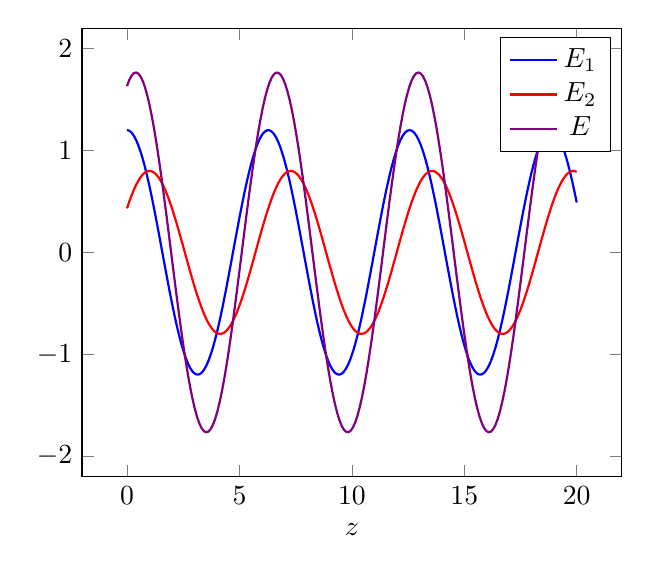
\begin{tikzpicture}
            \begin{axis}[
                xlabel=\(z\),
                domain=0:20,
                ymin=-2.2,
                ymax=2.2,
                samples=200
            ]
                \addplot[color=blue, thick] {1.2*cos(deg(x))};
                \addlegendentry{\(E_1\)}
                \addplot[color=red, thick] {0.8*cos(deg(x - 1))};
                \addlegendentry{\(E_2\)}
                \addplot[color=red!50!blue, thick] {1.2*cos(deg(x)) + 0.8*cos(deg(x - 1))};
                \addlegendentry{\(E\)}
            \end{axis}
        \end{tikzpicture}
        \caption{A snapshot at some fixed time \(t\) showing two harmonic waves, \(E_i\), with the same wave vector but different amplitudes and phases and their superposition, \(E\). Notice that \(E\) is a harmonic wave.}
        \label{fig:superposition same k and omega}
    \end{figure}

    Now that we have seen the superposition of two harmonic waves with the same frequency and wave vector the superposition of \(N\) harmonic waves all with the same frequency and wave vector is simply given by
    \[E = \sum_{i=1}^{N} E_{0i}\cos(kz - \omega t - \Phi_{i}) = E_0\cos(kz - \omega t - \Phi).\]
    
    \subsection{Alternative Computations}
    We computed the superposition using lots of trig identities.
    This is perhaps the slowest and least enlightening way to compute superpositions.
    The most efficient way is probably using complex exponentials and simply discarding the imaginary part when we need the actual physical wave.
    The starting waves are then given by
    \[E_i = E_{0i}\exp[i(kz - \omega t - \Phi_i)] = E_{01}\exp(-i\Phi_i)\exp[i(kz - \omega t)].\]
    The superposition of two waves is then
    \[E = E_1 + E_2 = E_0\exp(-i\Phi)\exp[i(kz - \omega t)]\]
    where \(E_0\) and \(\Phi\) are given in equation~\ref{eqn:E0 and Phi}.
    
    The same computation can also be done graphically with phasors which are simply vectors in the complex plane (viewed as a two dimensional real vector space) and we then simply perform normal vector addition to get the amplitude and phase which are simply the magnitude and angle of the resulting vector.
    See figure~\ref{fig:phasor addition}
    \begin{figure}[ht]
        \centering
        \tikzsetnextfilename{phasor-addition}
        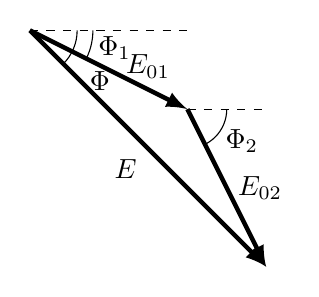
\begin{tikzpicture}
            \tikzset{vector/.style={ultra thick, ->, >=latex}}
            \draw[vector] (0, 0) -- (2, -1) node[pos=0.75, above] {\(E_{01}\)};
            \draw[vector] (2, -1) -- (3, -3) node[midway, right] {\(E_{02}\)};
            \draw[vector] (0, 0) -- (3, -3) node[midway, below left] {\(E\)};
            \draw[dashed] (0, 0) -- (2, 0);
            \draw[dashed] (2, -1) -- (3, -1);
            \begin{scope}
                \clip (0, 0) -- (2, -1) -- (2, 0) -- cycle;
                \draw (0, 0) circle[radius=0.8cm];
            \end{scope}
            \begin{scope}
                \clip (2, -1) -- (3, -3) -- (3, -1) -- cycle;
                \draw (2, -1) circle[radius=0.5cm];
            \end{scope}
            \begin{scope}
                \clip (0, 0) -- (3, -3) -- (3, 0);
                \draw (0, 0) circle[radius=0.6cm];
            \end{scope}
            \node at (-12:1.1) {\(\Phi_1\)};
            \begin{scope}[xshift=2cm, yshift=-1cm]
                \node at (-30:0.8) {\(\Phi_2\)};
            \end{scope}
            \node at (-36:1.1) {\(\Phi\)};
        \end{tikzpicture}
        \caption{Addition of two phasors.}
        \label{fig:phasor addition}
    \end{figure}
    
    \subsection{Intensities}
    The intensity of the field is proportional to the amplitude squared.
    In fact \(I = v\varepsilon E_0^2/2\) however it is common to just work with \(I = E_0^2\) when we only want to compare intensities within a single medium.
    From equation~\ref{eqn:E0 and Phi} we see that
    \[E_0^2 = E_{01}^2 + E_{02}^2 + 2E_{01}E_{02}^2\cos(\Phi_{1} - \Phi_{2}).\]
    So the total intensity is the sum of the intensities plus an interference term which may be positive or negative depending on how in phase the waves are.
    
    The maximum (resp. minimum) intensity is achieved when the phase difference \(\Phi_1 - \Phi_2\) is an even (resp. odd) multiple of \(\pi\) and we have
    \[E_{0}^2{_{\min\mkern-4mu/\mkern-4mu\max}} = E_{01}^2 + E_{02}^2 \pm 2E_{01}E_{02} = (E_{01} \pm E_{02})^2.\]
    So for the special case of \(E_{01} = E_{02}\) it is possible that the intensity of the resulting wave will be anywhere from 0 to \(4E_{01}\).
    
    \subsection{Phases}
    There are a few mechanisms by which a phase difference can appear:
    \begin{itemize}
        \item The first crests of the two waves leave the emitters at different times by a non-integer multiple of the period.
        \item The two emitters are a non-integer number of wavelengths apart.
        \item The two waves start in phase but then one passes through a more optically dense material.
    \end{itemize}
    To be rigorous about the third of these we introduce the idea of an \define{phase thickness} which is defined to be
    \[\delta = \frac{2\pi d}{\lambda}\]
    where \(d\) is the actual thickness of the material and \(\lambda\) is the wavelength of the light in the medium.
    In terms of the vacuum wavelength, \(\lambda_0\), we have
    \[\delta = \frac{2\pi nd}{\lambda_0}.\]
    This quantity is related to the optical thickness, \(nd\), but the phase thickness accounts for the phase difference between light that travels through the medium and the same light if it had been unimpeded.
    If the difference in phase thickness is caused purely by a difference in refractive indices then it is sometimes referred to as \define{retardation}.
    
    \subsection{Coherence}
    We have so far assumed that the phase difference, \(\Phi_1 - \Phi_2\), is constant.
    We will see later that this isn't always the case and we will introduce notions of coherence time and coherence length which are scales over which the phase difference is approximately constant.
    
    \section{More Superposition}
    \subsection{Standing Waves}
    Suppose two waves of the same frequency, \(\omega\), are travelling in opposite directions with different amplitudes.
    The resultant field has amplitude
    \[E(z, t) = E_{0L}\cos(kz - \omega t) + E_{0R}\cos(kz + \omega t).\]
    If \(E_{0L} = E_{0R}\) then some basic trig identities lead us to conclude that
    \[E(z, t) = 2E_{0L}\cos(kz)\cos(\omega t).\]
    This is different to waves we have studied so far in that it is not of the form \(f(z \pm vt)\) or \(f(kz \pm \omega t)\).
    Instead we have oscillations based on position, \(z\), and oscillations with time, \(t\).
    All points in the wave rise and fall at the same time.
    This is a \define{standing wave}.
    
    It can be shown that for a standing wave the magnetic field is
    \[B(z, t) = \frac{E(z', t')}{c}\]
    where \(z' = z - \lambda/4\) and \(t' = t - T/4\) which corresponds to \(\vv{B}\) and \(\vv{E}\) being perpendicular but put of phase by \(\pi/2\).
    An important quantity for standing waves is the Poynting vector, \(\vv{S} = \vv{E}\times\vv{B}\).
    This calculation is complicated by the fact that \(\vv{B} \ne \vv{E}/c\) which we have relied on in the past.
    It can be shown that
    \[\vv{S} = c\varepsilon_0E_0^2 \sin(2kz)\sin(2\omega t)\ve{z}.\]
    So \(\vv{S}\) is always along the \(z\) direction but its amplitude and sign oscillate in time and space in such a way that
    \[I = \expected{S} = 0.\]
    So for a standing wave there is no flow of energy.
    There is movement of energy but it moves forward and back so the net result is no energy flow.
    
    \subsection{Superposition with Similar Frequencies}
    Consider two waves that are \emph{almost} the same.
    For example these waves may be produced by the same source and have the same amplitude, \(E_{01}\), but slightly different wave vectors and frequencies.
    These waves are given by
    \[E_1 = E_{01}\cos(k_iz - \omega_i t).\]
    We can use the trig identity
    \[\cos\alpha + \cos\beta = 2 \cos\left( \frac{1}{2}(\alpha + \beta) \right)\cos\left( \frac{1}{2}(\alpha - \beta) \right).\]
    The superposition of these waves is then
    \[E = 2E_{01} \cos\left[ \left( \frac{k_1 + k_2}{2}z - \left( \frac{\omega_1 - \omega_2}{2} \right) \right) \right] \cos\left[ \left( \frac{k_1 - k_2}{2} \right)z - \left( \frac{\omega_1 - \omega_2}{2} \right)t \right].\]
    Notice that this appears to be the product of two different waves.
    We call the first the \define{carrier} wave and it has frequency and wave vector
    \[\omega_c = \frac{\omega_1 + \omega_2}{2}, \qquad\text{and}\qquad k_c = \frac{k_1 + k_2}{2}.\]
    The second is called the \define{modulation} wave and it has frequency and wave vector
    \[\omega_m = \frac{\omega_1 - \omega_2}{2}, \qquad\text{and}\qquad k_m = \frac{k_1 - k_2}{2}.\]
    So the resulting wave is
    \[E = 2E_{01}\cos(k_cz - \omega_ct)\cos(k_mz - \omega_t).\]
    Since \(\omega_1 \approx \omega_2\) and \(k_1 \approx k_2\) we have that \(\omega_c \gg \omega_m\) and \(k_c \gg k_m\).
    The result is a wave with approximate frequency and wave vector \(\omega_c\) and \(k_c\) which is attenuated by a wave with frequency \(\omega_m\) and wave vector \(k_m\).
    This can be seen in figure~\ref{fig:carrier and modulating wave}.
    
    \begin{figure}[htp]
        \centering
        \tikzsetnextfilename{superposition-carrier-and-modulating-wave}
        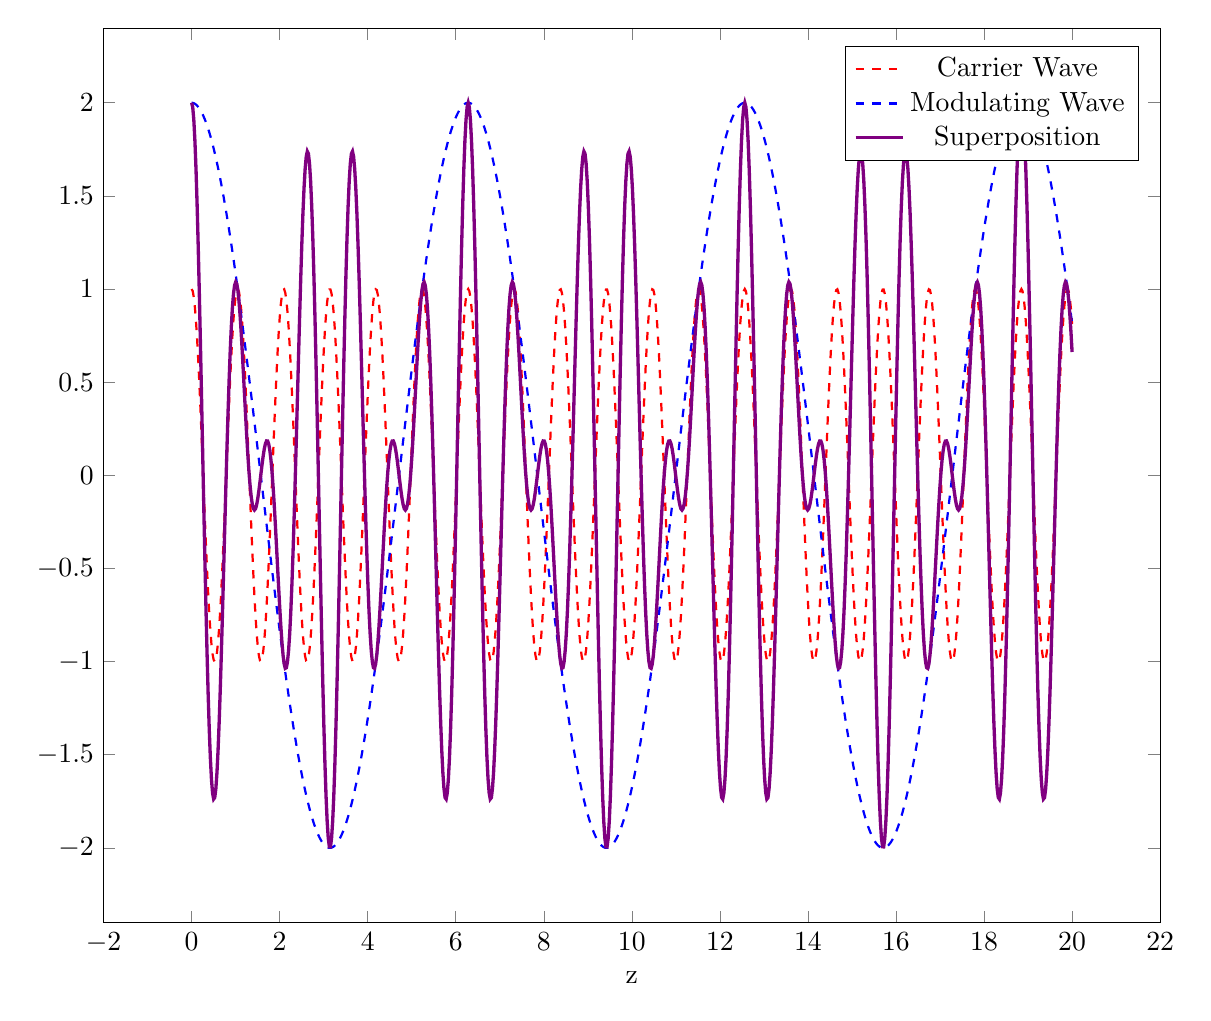
\begin{tikzpicture}
            \begin{axis}[
                domain=0:20,
                xlabel=z,
                samples=800,
                width=15cm
            ]
                \addplot[thick, red, dashed] {cos(deg(6*x))};
                \addlegendentry{Carrier Wave}
                \addplot[thick, blue, dashed] {2*cos(deg(x))};
                \addlegendentry{Modulating Wave}
                \addplot[very thick, red!50!blue] {2*cos(deg(6*x))*cos(deg(x))};
                \addlegendentry{Superposition}
            \end{axis}
        \end{tikzpicture}
        \caption{The superposition of two waves with similar frequency and wave vector results in a carrier wave attenuated by a lower frequency wave.}
        \label{fig:carrier and modulating wave}
    \end{figure}
    The intensity of this wave is found by averaging \(\abs{\vv{S}}\) over one period of the carrier wave.
    This gives
    \[I \propto 4E_{01}^2\cos^2(k_mz - \omega_mt) = 2E_{01}^2[1 + \cos(2(k_mz - \omega_mt))].\]
    We see that the intensity varies from 0 to \(4E_{01}^2\) with frequency \(2\omega_{m}\), which is known as the beats frequency.
    We can actually hear the beats frequency if we choose two notes close in frequency but differing by a few hertz.
    
    \subsubsection{Group and Phase Velocity}
    The dispersion of electromagnetic waves in media leads to different phase velocities at different frequencies.
    Notice we introduce the modifier here `phase' as we will see there is a second velocity of interest in this scenario.
    
    The modulation wave moves with velocity \(v_m\) given by the dispersion relationship:
    \[v_m = \frac{\omega_m}{k_m} = \frac{\omega_1 - \omega_2}{k_1 - k_2} = \frac{\Delta \omega}{\Delta k}.\]
    Assuming that \(\omega_c \gg \omega_m\), i.e. that \(\omega_1 \approx \omega_2\) and similarly \(k_c \gg k_m\) this ratio of differences can be approximated with a derivative:
    \[v_g = \dv{\omega}{k}\]
    where \(v_g\) is known as the \define{group velocity} and is the velocity of the envelope (modulation wave).
    We can relate the group velocity and the phase velocity (which up until this point we have simply referred to as velocity) by noting that \(\omega = ck/n\) and also refractive index depends on frequency so \(n = n(\omega)\) which means that
    \[\omega = \frac{ck}{n(\omega)} = v_p(\omega)k.\]
    Differentiating this and rearranging we get
    \[v_g = \dv{\omega}{k} = \frac{1}{n + \omega \inlinedv{n}{\omega}} = \frac{v_p}{1 - (\omega/v_p)\inlinedv{v_p}{\omega}}.\]
    One interesting consideration here is that it is possible that \(v_p\) can be greater than \(c\).
    This seems to disagree with special relativity but it turns out that no information can be transmitted at the phase velocity, the only way information can be sent in this case is in the resulting wave which travels at the group velocity, which is always lower than \(c\).
    So special relativity isn't violated.
    
    \section{Fourier Analysis}
    Up until now in this part we have taken two (or more) waves and computed the resulting field.
    In this section we will look at the resulting wave and attempt to recover the individual waves.
    Assuming that the only waves present are harmonic we can do this using Fourier analysis.
    
    
    Consider some periodic wave, \(f\), which is not necessarily harmonic.
    By periodic we mean there exists some \(\lambda\in\reals\) such that \(f(z) = f(z + \lambda)\).
    Then we can decompose \(f\) (under some fairly week conditions) as
    \[f(z) = \frac{A_0}{2} + \sum_{m=1}^{\infty} A_m\cos(mkz) + \sum_{m=1}^{\infty} \sin(mkz)\]
    where \(k = 2\pi/\lambda\), and \(A_m\) and \(B_m\) are real constants given by
    \[A_m = \frac{2}{\lambda} \int_{0}^{\lambda} f(z) \cos(mkz)\dd{z}, \qquad\text{and}\qquad B_m = \frac{2}{\lambda}\int_{0}^{\lambda} f(z)\sin(mkz)\dd{z}.\]
    
    For a non-periodic wave we can consider it to be a periodic function which repeats at infinity.
    A proper limiting process\footnote{See the Fourier analysis part of the Fourier analysis and statistics course} gives us
    \[f(z) = \frac{1}{\pi} \left[ \int_{0}^{\infty} A(k)\cos(kz)\dd{k} + \int_{0}^{\infty} B(k)\sin(kz)\dd{k} \right]\]
    where \(A\) and \(B\) are now functions of \(k\in\reals\)
    
    \begin{example}
        Consider the function \(f\), defined by
        \[
            f(z) =
            \begin{cases}
                1/L, & \text{if}~z\in[-L/2, L/2],\\
                0, & \text{else}.
            \end{cases}
        \]
        The Fourier transform of this is
        \begin{align*}
            \hat{f}(k) &= \FT[f](k) \\
            &= \int_{-\infty}^{\infty} f(z)e^{-ikz}\dd{z}\\
            &= \frac{1}{L}\int_{-L/2}^{L/2} [\cos(kz) + i\sin(kz)]\dd{z}\\
            &= \frac{1}{Lk}[\sin(kz)]_{-L/2}^{L/2}\\
            &= \frac{1}{Lk}\sin\left( \frac{kL}{2} \right) - \frac{1}{Lk}\sin\left( -\frac{kL}{2} \right)\\
            &= \frac{2}{Lk}\sin\left( \frac{kL}{2} \right)\\
            &=\sinc\left( \frac{kL}{2} \right)
        \end{align*}
        where \(\sinc\) is the un-normalised \(\sinc\) function defined as
        \[
            \sinc x =
            \begin{cases}
                \frac{\sin x}{x}, & x \ne 0,\\
                1, & x = 0.
            \end{cases}
        \]
        The untransformed function, \(f\), has width \(L\) and the transformed function, \(\hat{f}\), has width \(4\pi/L\) (width here being the distance between the first two zeros) so the width of \(f\) is inversely proportional to the width of \(\hat{f}\).
        This is known as the reciprocal relation and is common in Fourier analysis.
    \end{example}
    \begin{example}
        Another important example of a Fourier transform is a Gaussian with variance \(\sigma^2 = 2L\) and mean \(\mu = 0\).
        The Fourier transform is again a Gaussian with \(\mu = 0\) but now \(\sigma^2 = 2\pi/L\), which again shows the reciprocal relation.
    \end{example}
    \begin{example}
        The Dirac delta distribution is defined by
        \[
            \delta(x) =
            \begin{cases}
                0, & x \ne 0\\
                \infty, & x = 0,
            \end{cases}
        \]
        and\footnote{Here \(1_X\) is the indicator function defined by \(1_X(x) = 1\) if \(x \in X\) and \(1_X(x) = 0\) if \(x \notin X\).}
        \[
            \int_{a}^{b} \delta(x) \dd{x} = 1_{(a, b)}(0) =
            \begin{cases}
                1, & 0\in (a, b),\\
                0, & 0\notin (a, b).
            \end{cases}
        \]
        It has the property that
        \[
            \int_{a}^{b} f(x) \delta(x - x')\dd{x} = 
            \begin{cases}
                f(x'), & x'\in (a, b),\\
                0, & x'\notin (a, b).
            \end{cases}
        \]
        This sifting property makes it very easy to compute the Fourier transform:
        \begin{align*}
            \hat{\delta}(k) &= \FT[\delta](x - x')\\
            &= \int_{-\infty}^{\infty} \delta(x - x')e^{-ikx}\dd{x}\\
            &= e^{ikx'}.
        \end{align*}
        Notice that \(\delta\) has zero width and \(\hat{\delta}\) has infinite width.
    \end{example}

    Some useful properties of the Fourier transform that can simplify computations are
    \begin{itemize}
        \item If \(f\) is an even function then \(\FT[f]\) is real.
        \item If \(f\) is an odd function then \(\FT[f]\) is imaginary.
        \item The Fourier transform of the Fourier transform of \(f\) is the mirror image of \(f\).
        This means \(\FT\{f(z)\} = 2\pi\FT^{-1}\{f(-z)\}\).
        \item \(\FT\) is a linear operator so \(\FT\{af(z) + bg(z)\} = a\FT\{f(z)\} + b\FT\{g(z)\}\).
        \item If \(f\) is wide then \(\FT\{f\}\) is narrow.
        In particular if \(f\) has width \(L\) then \(\FT\{f\}\) has width proportional to \(1/L\).
        \item Convolution in real space becomes multiplication in Fourier space:
        \[h(z) = (f\convolution g)(z) = \int_{-\infty}^{\infty} f(x - x')g(x') \dd{x'} \iff h(z) = \FT{}^{-1}\{\FT[f]\FT[g]\}(z).\]
    \end{itemize}
    The linearity property and the inverse Fourier transform property allow us to identify
    \[\FT\{\cos(k_0z)\} = \delta(k - k_0) + \delta(k + k_0).\]
    We will use this later.
    
    \subsection{Wave Packets}
    Until now we have mostly considered harmonic waves that extend forever in time and space.
    This is unrealistic but good enough in some cases.
    A more realistic case would be a wave that starts and finishes at some fixed time.
    A snapshot of this wave may look like
    \begin{center}
        \tikzsetnextfilename{wave-with-finite-extent}
        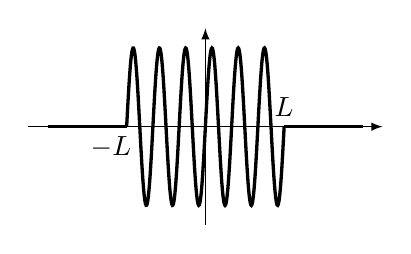
\begin{tikzpicture}
            \draw[->, >=latex] (-0.25, 0) -- (4.25, 0);
            \draw[->, >=latex] (2, -1.25) -- (2, 1.25);
            \draw[very thick] (0, 0) -- (1, 0);
            \draw[domain=0:2, xshift=1cm, samples=300, very thick] (0, 0) -- plot(\x, {sin(6*pi*\x r)}) -- (2, 0);
            \draw[very thick] (3, 0) -- (4, 0);
            \node[below] at (0.8, 0) {\(-L\)};
            \node[above] at (3, 0) {\(L\)};
        \end{tikzpicture}
    \end{center}
    We can consider this to be the product of a top hat and a harmonic wave:
    \[
        \tikzsetnextfilename{wave-with-finite-extent-1}
        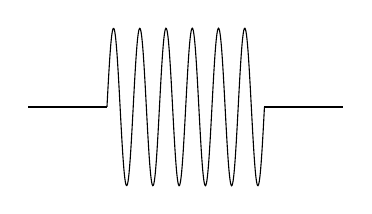
\begin{tikzpicture}[baseline=0, yshift=\axisht]
            \draw (0, 0) -- (1, 0);
            \draw[domain=0:2, xshift=1cm, samples=300] (0, 0) -- plot(\x, {sin(6*pi*\x r)}) -- (2, 0);
            \draw (3, 0) -- (4, 0);
        \end{tikzpicture}
        \quad=\quad
        \tikzsetnextfilename{wave-top-hat}
        \begin{tikzpicture}[baseline=0, yshift=\axisht]
            \draw (0, 0) -- (1, 0) -- (1, 1) -- (3, 1) -- (3, 0) -- (4, 0);
        \end{tikzpicture}
        \quad\times\quad
        \tikzsetnextfilename{wave-harmonic}
        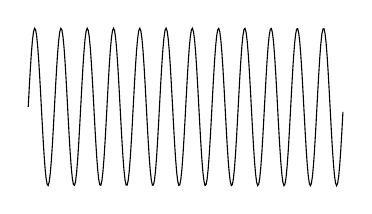
\begin{tikzpicture}[baseline=0, yshift=\axisht]
            \draw[domain=1:5, samples=300] plot(\x, {sin(6*pi*\x r)});
        \end{tikzpicture}
    \]
    The Fourier transform of this can then be computed using the convolution theorem:
    \begin{align*}
        \FT\,
        \tikzsetnextfilename{wave-with-finite-extent-2}
        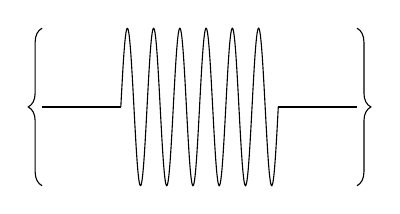
\begin{tikzpicture}[baseline=0, yshift=\axisht]
            \draw[decorate, decoration={brace, amplitude=5pt}] (0, -1) -- (0, 1);
            \draw (0, 0) -- (1, 0);
            \draw[domain=0:2, xshift=1cm, samples=300] (0, 0) -- plot(\x, {sin(6*pi*\x r)}) -- (2, 0);
            \draw (3, 0) -- (4, 0);
            \draw[decorate, decoration={brace, amplitude=5pt}] (4, 1) -- (4, -1);
        \end{tikzpicture}
        \quad&= \FT\,
        \tikzsetnextfilename{wave-top-hat-1}
        \begin{tikzpicture}[baseline=0, yshift=\axisht]
            \draw[decorate, decoration={brace, amplitude=5pt}] (0, -1) -- (-0, 1);
            \draw (0, 0) -- (1, 0) -- (1, 1) -- (3, 1) -- (3, 0) -- (4, 0);
        \end{tikzpicture}
        \quad\times\quad
        \tikzsetnextfilename{wave-harmonic-1}
        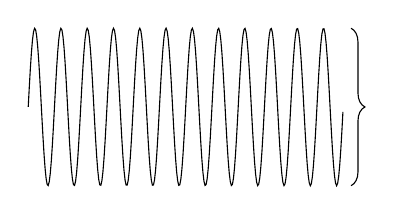
\begin{tikzpicture}[baseline=0, yshift=\axisht]
            \draw[domain=1:5, samples=300] plot(\x, {sin(6*pi*\x r)});
            \draw[decorate, decoration={brace, amplitude=5pt}] (5.1, 1) -- (5.1, -1);
        \end{tikzpicture}
        \\
        &= \FT\, \tikzsetnextfilename{wave-top-hat-2}
        \begin{tikzpicture}[baseline=0, yshift=\axisht]
            \draw[decorate, decoration={brace, amplitude=5pt}] (0, -1) -- (0, 1);
            \draw (0, 0) -- (1, 0) -- (1, 1) -- (3, 1) -- (3, 0) -- (4, 0);
            \draw[decorate, decoration={brace, amplitude=5pt}] (4, 1) -- (4, -1);
        \end{tikzpicture}
        \;\convolution\,\FT\,
        \tikzsetnextfilename{wave-harmonic-2}
        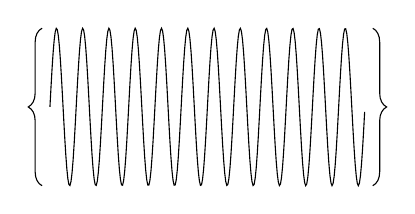
\begin{tikzpicture}[baseline=0, yshift=\axisht]
            \draw[decorate, decoration={brace, amplitude=5pt}] (-0.1, -1) -- (-0.1, 1);
            \draw[domain=1:5, samples=300, xshift=-1cm] plot(\x, {sin(6*pi*\x r)});
            \draw[decorate, decoration={brace, amplitude=5pt}] (4.1, 1) -- (4.1, -1);
        \end{tikzpicture}
    \end{align*}
    We can define units such that the wave starts at \(-L\) and ends at \(L\).
    We see that in the time it exists there are 6 full cycles of the wave.
    The wave length is \(\lambda_0 = 2L/6\).
    Hence the wave vector is \(k_0 = 2\pi/\lambda_0 = 6\pi/L\).
    Working in units of \(L\) we have
    \begin{align*}
        \hat{f}(k) &= \sinc(k) \convolution [\delta(k - k_0) + \delta(k + k_0)]\\
        &= \int_{-\infty}^{\infty} \sinc(k - k') \delta(k' - k_0)\dd{k'} + \int_{-\infty}^{\infty} \sinc(k - k') \delta(k' + k_0)\dd{k'}\\
        &= \sinc(k - k_0) + \sinc(k + k_0).
    \end{align*}
    
    We can similarly show that for a Gaussian wave packet, that is a wave of the form
    \[\cos(k_0z) \exp[-z^2/(2\sigma^2)]\]
    the Fourier transform is, up to a constant factor,
    \[\exp[-k^2\sigma^2/2].\]
    The important thing about both of these wave packets is that the Fourier transforms are \emph{not} delta distributions.
    This means that there is more than one frequency present.
    We conclude that a wave of finite extent cannot be monochromatic.
    Instead it has many wave vectors with the most important being those near \(k = k_0\) since this is where \(\sinc\)/the Gaussian peaks.
    
    \subsection{Band Width}
    The following result follows from the reciprocal relationship:
    \[\Delta x\Delta k \propto L \frac{1}{L} \propto 1.\]
    The more general relationship is
    \[\Delta x\Delta k \ge 1\]
    with equality only for Gaussians.
    This relationship appears all over the place in physics.
    For example the uncertainty principle is essentially the same with momentum, \(p = \hbar k\) replacing \(k\) and applied to the probability density, \(\abs{\psi}^2\).
    This is a consequence of the wavelike nature of matter.
    
    In the last section we considered a wave with finite extent in space.
    The exact same analysis applies to a wave with finite extent in time replacing \(x\) with \(t\) and \(k\) with \(\omega\) so we have
    \[\Delta t\Delta\omega \ge 1.\]
    The value \(\Delta t\) is known as the \define{coherence time} and \(\Delta x = c\Delta t\) is the \define{coherence length}.
    These quantities give the time scales and length scales over which the phase relationship between two waves is approximately constant.
    For larger time periods/lengths the phase relationship is essentially random.
    
    \subsection{Group Velocity Again}
    Consider a wave packet, \(\psi(z, t)\), with Fourier transform at time \(t = 0\) given by \(\Psi\) so
    \[\psi(z, 0) = \FT^{-1}\{\Psi(k)\} = \int_{-\infty}^{\infty} \Psi(k)e^{-ikz} \dd{k}.\]
    At some later time all components of the wave will have propagated at the phase velocity \(\omega(k)/k\) and so
    \[\psi(z, t) = \int_{-\infty}^{\infty} \Psi(k)e^{-i(kz - \omega t)} \dd{k}.\]
    As long as the wave packets all have wave vectors close to \(k_0\) we can approximate \(\omega(k)\) to first order by
    \[\omega(k) \approx \omega(k_0) + (k - k_0)\dvat{\omega}{k}{k_0} = \omega_0 + (k - k_0)v_g.\]
    Hence we have
    \begin{align*}
        \psi(z, t) &= e^{-i(v_gk_0 - \omega_0)t} \int_{-\infty}^{\infty} \Psi(k)e^{-i(kz - kv_g t)}\dd{k}\\
        &= e^{-i(v_gk_0 - \omega_0)t} \psi(z - v_gt, 0).
    \end{align*}
    So we see that wave packets with wave vectors centred on \(k_0\) travel at the group velocity, \(v_g\).
    
    \part{Polarisation}
    \section{Polarisation}
    So far we have considered superposition of waves travelling along the \(z\)-axis with \(\vv{E}\) aligned and \(\vv{B}\) aligned an perpendicular to \(\vv{E}\).
    This isn't always the case and to generalise we need to look at polarised light.
    
    \subsection{Linear Polarisation}
    Consider the two following waves
    \[\vv{E_1} = \ve{x}E_{0x}\cos(kz - \omega t - \Phi_1), \qquad\text{and}\qquad \vv{E_2} = \ve{y}E_{0y}\cos(kz - \omega t - \Phi_2).\]
    The first of these is \(x\)-polarised as the electric field oscillates only along the \(x\)-axis, the second is \(y\)-polarised.
    We can write these as complex exponentials discarding the imaginary parts for the final values:
    \[\vv{E_1} = \ve{x}E_{0x}\exp[i(kz - \omega t - \Phi_1)], \qquad\text{and}\qquad \vv{E_2} = \ve{y}E_{0y}\exp[i(kz - \omega t - \Phi_2)].\]
    The superposition is then given by the sum of these two vectors:
    \[\vv{E} = \vv{E_1} + \vv{E_2}= \ve{x}E_{0x}\exp[i(kz - \omega t - \Phi_1)] + \ve{y}E_{0y}\exp[i(kz - \omega t - \Phi_2)].\]
    We can write these in terms of column vectors with the first component giving the \(x\) component and the second the \(y\) component:
    \[
        \vv{E} =
        \begin{pmatrix}
            E_{0x}\exp[i(kz - \omega t - \Phi_1)]\\
            E_{0y}\exp[i(kz - \omega t - \Phi_2)]
        \end{pmatrix}
        =
        \begin{pmatrix}
            E_{0x}e^{-i\Phi_1}\\
            E_{0y}e^{-i\Phi_2}
        \end{pmatrix}
        \exp[i(kz - \omega t)].
    \]
    Notice that we separate the oscillatory term into the exponential outside the vector and the vector is constant in time.
    This vector is called the \define{Jones vector} for \(\vv{E}\).
    The Jones vector is simply the complex amplitudes of the components of the wave in the \(x\) and \(y\) directions.
    
    \subsubsection{No Phase Shift}
    Suppose there is no relative phase shift between the two components.
    That is \(\Phi_1 = \Phi_2 = \Phi\), then
    \[
        \vv{E} = 
        \begin{pmatrix}
            E_{0x}\\ E_{0y}
        \end{pmatrix}
        e^{-i\Phi}\exp[i(kz - \omega t)].
    \]
    We can then identify \(\vv{E}\) as another linearly polarised wave with amplitude
    \[E_{0} = \sqrt{E_{0x}^2 + E_{0y}^2}\]
    which is polarised at angle
    \[\vartheta = \arctan\left( \frac{E_{0y}}{E_{0x}} \right)\]
    to the \(x\)-axis.
    
    \subsubsection{Circularly Polarised Light}
    Suppose the two waves have a constant phase difference of \(\pi/2\) so \(\Phi_1 - \Phi_2 = \pi/2\).
    Suppose also that \(E_{0x} = E_{0y} = E_{01}\).
    Then
    \[
        \vv{E} = 
        \begin{pmatrix}
            E_{01}e^{-i(\Phi_2 + \pi/2)}\\
            E_{01}e^{-i\Phi_2}
        \end{pmatrix}
        \exp[i(kz - \omega t)] = 
        \begin{pmatrix}
            -i\\ 1
        \end{pmatrix}
        e^{-i\Phi_2}\exp[i(kz - \omega t)].
    \]
    It is fairly easy to show that as \(z\) increases \((E_x(z), E_y(z))\) maps out a clockwise circle completing one circle each time \(z\) increases by one wavelength.
    Similarly \((E_x(t), E_y(t))\) maps out an anticlockwise circle with angular frequency \(\omega\).
    This is a circularly polarised state.
    We call this \define{left hand circularly polarised}, or \(\mathcal{L}\).
    Similarly if \(\Phi_1 - \Phi_2 = -\pi/2\) then we have Jones vector
    \[
        \begin{pmatrix}
            i\\ 1
        \end{pmatrix}
    \]
    and the circles are in the opposite direction.
    We call this \define{right hand circularly polarised}, or \(\mathcal{R}\).
    
    \subsubsection{Elliptically Polarised}
    The most general case has no relationship between amplitudes or phases.
    Then \(\vv{E}\) both rotates and changes magnitude in the \((x, y)\)-plane tracing out an ellipse as it does so competing one rotation every wave length with angular frequency \(\omega\).
    We call this \define{elliptically polarised light}.
    
    \subsection{Normalisation}
    As is often the case with vectors we wish to work with orthonormal vectors as a basis.
    For this we need a well defined inner product.
    Since the polarisation vectors are two dimensional and contain complex values we can identify them with \(\complex^2\) and the correct inner product is then
    \[
        \vv{a} \cdot \vv{b} = \vv{a}\hermit\vv{b} =
        \begin{pmatrix}
            a_1\\ a_2
        \end{pmatrix}
        \hermit
        \begin{pmatrix}
            b_1\\ b_2
        \end{pmatrix}
        =
        \begin{pmatrix}
            a_1^* & a_2^*
        \end{pmatrix}
        \begin{pmatrix}
            b_1\\ b_2
        \end{pmatrix}
        = a_1^*b_1 + a_2^*b_2.
    \]
    In particular we say that \(\{\ve{i}\}\) are orthonormal if \(\ve{i}\cdot\ve{j} = \delta_{ij}\).
    
    Clearly the vectors denoting \(x\) and \(y\) polarised light,
    \[
        \ve{x} = 
        \begin{pmatrix}
            1\\ 0
        \end{pmatrix}
        , \qquad\text{and}\qquad \ve{y} = 
        \begin{pmatrix}
            0\\ 1
        \end{pmatrix}
    \]
    are orthonormal.
    The vectors that we found for describing circularly polarised light are orthogonal and can be normalised by a factor of \(1/\sqrt{2}\):
    \begin{equation}\label{eqn:circular basis}
        \ve{\mathcal{R}} = \frac{\sqrt{2}}{2}
        \begin{pmatrix}
            i\\ 1
        \end{pmatrix}
        , \qquad\text{and}\qquad \ve{\mathcal{L}} = \frac{\sqrt{2}}{2}
        \begin{pmatrix}
            i\\ -1
        \end{pmatrix}
        .
    \end{equation}
    In order to be a proper basis a set must span the space while being linearly independent.
    This is known to be true for \(\{\ve{x}, \ve{y}\}\) and is easy to show for \(\{\ve{\mathcal{R}}, \ve{\mathcal{L}}\}\) since \(\ve{\mathcal{R}} + \ve{\mathcal{L}} = i\sqrt{2}\ve{x}\) and \(\ve{\mathcal{R}} - \ve{\mathcal{L}} = i\sqrt{2}\ve{y}\) so as long as \(\{\ve{x}, \ve{y}\}\) spans the space \(\{\ve{\mathcal{R}}, \ve{\mathcal{L}}\}\) spans the space too meaning both are orthonormal bases.
    Which basis we use depends on the types of polarisation present.
    
    \subsection{Intensity}
    The electric field can be written as
    \[
        \vv{E} = 
        \begin{pmatrix}
            E_{0x}e^{-i\Phi_1}\\
            E_{0y}e^{-i\Phi_2}
        \end{pmatrix}
        \exp[i(kz - \omega t)] = \vv{E_0} \exp[i(kz - \omega t)].
    \]
    The intensity is given by the square of the magnitude of the electric field.
    Since we deal with the complex amplitude here this is
    \[I = \frac{1}{2}c\varepsilon_0E_0 \abs{E_0}^2 = \frac{1}{2}c\varepsilon_0\vv{E_0}\cdot\vv{E_0} = \frac{1}{2}c\varepsilon_0E_0^*E_0 = \frac{1}{2}c\varepsilon_0(E_{0x}^2 + E_{0y}^2).\]
    
    \section{Polarisers}
    Any individual wave has a polarisation however most light is formed of many different waves which are incoherent and, on average, have no net polarisation.
    For this reason we need a way to produce polarised light.
    
    \subsection{Linear Polarisers}
    A \define{linear polariser} (often just called a polariser) will only allow light polarised along a fixed axis to pass through.
    Natural (unpolarised) light has the form
    \[
        \begin{pmatrix}
            E_x(z, t)\\
            E_y(z, t)
        \end{pmatrix}
        =
        \begin{pmatrix}
            E_{0x}(t)\cos[kz - \omega t - \Phi_x(t)]\\
            E_{0y}(t)\cos[kz - \omega t - \Phi_y(t)]
        \end{pmatrix}
        .
    \]
    In general the two components are only coherent over short time scales, less than the coherence time, \(\Delta t\).
    Over time scales larger than this the ratio of the amplitudes, \(E_{0x}/E_{0y}\), and the relative phase, \(\Phi_y - \Phi_x\), will be unpredictable.
    If this light passes through a polariser then this forces a correlation between the amplitudes and phases and therefore the resulting light will be coherent and the output from the polarised behaves like an ideal harmonic wave.
    For this reason it is common to use a polariser as the first step in an optics experiment.
    
    \subsection{Malus's Law}
    Consider light from one polariser passing through a second polariser.
    If the axes of polarisation are aligned then we expect that all light from the first polariser will pass through the second.
    If the axes of polarisation are perpendicular then we expect the second polariser to block all of the light.
    What happens if the axes are not parallel or perpendicular?
    
    Suppose that the first polariser produces light, \(\vv{E_{\mathrm{in}}}\), and that the axis of the second polariser, \(\vh{p}\), is at angle \(\vartheta\) to the polarisation of the incoming light.
    The light transmitted through the second polariser, \(\vv{E_{\mathrm{out}}}\), is the component of \(\vv{E_{\mathrm{in}}}\) in the direction of \(\vh{p}\), and is polarised in the direction \(\vh{p}\).
    That is
    \[\vv{E_{\mathrm{out}}} = (\vv{E_{\mathrm{in}}}\cdot\vh{p})\vh{p} = E_{\mathrm{in}}\cos(\vartheta)\vh{p}.\]
    The intensity of the light coming from the second polariser is then
    \[I_{\mathrm{out}}(\vartheta) = \frac{1}{2}c\varepsilon_0E_{\mathrm{in}}^2\cos^2\vartheta = I_{\mathrm{in}}\cos^2\vartheta.\]
    So as the second polariser is rotated we expect the intensity of the output to go as \(\cos^2\vartheta\).
    This is \define{Malus's law}.
    Notice that in a whole rotation there are two maxima, \(\vartheta = 0, \pi\), which correspond to the polarisers being aligned and anti-aligned, and two minima, \(\vartheta = \pi/2, 3\pi/2\), which correspond to the two times the polarisers are perpendicular.
    
    \subsection{Jones Matrices}
    We managed to find the intensity in the last section by a logical argument.
    However there is a much more powerful mathematical framework that allows us to work with arbitrary combinations of polarisers.
    This framework, called Jones matrices, assigns to each polariser a matrix which then acts on the Jones vector of the incoming light.
    A linear polariser in the \(x\) direction has the Jones matrix
    \[
        \begin{pmatrix}
            1 & 0\\
            0 & 1
        \end{pmatrix}
    \]
    since
    \[
        \begin{pmatrix}
            1 & 0\\
            0 & 1
        \end{pmatrix}
        \begin{pmatrix}
            E_{x}\\ E_{y}
        \end{pmatrix}
        =
        \begin{pmatrix}
            E_x\\ 0
        \end{pmatrix}
        ,
    \]
    so we are left with only the \(x\) component.
    Similarly a linear polariser in the \(y\) direction has Jones matrix
    \[
        \begin{pmatrix}
            0 & 0\\
            0 & 1
        \end{pmatrix}
        .
    \]
    From here we can construct the matrix for a polariser at arbitrary angle \(\vartheta\) by realising that this is really just a rotated version of an \(x\) aligned polariser.
    This is best demonstrated by considering the same example of incoming polarised light, which without loss of generality we assume to be \(x\) polarised, and a polariser at angle \(\vartheta\).
    Then
    \begin{align*}
        \vv{E_{\mathrm{out}}} &= 
        \begin{pmatrix}
            1 & 0\\
            0 & 1
        \end{pmatrix}
        R(\vartheta)
        \begin{pmatrix}
            1\\ 0
        \end{pmatrix}
        \\
        &= 
        \begin{pmatrix}
            1 & 0\\
            0 & 1
        \end{pmatrix}
        \begin{pmatrix}
            \cos\vartheta & -\sin\vartheta\\
            \sin\vartheta & \cos\vartheta
        \end{pmatrix}
        \begin{pmatrix}
            1\\ 0
        \end{pmatrix}
        \\
        &= 
        \begin{pmatrix}
            1 & 0\\
            0 & 1
        \end{pmatrix}
        R(\vartheta)
        \begin{pmatrix}
            \cos\vartheta\\ \sin\vartheta
        \end{pmatrix}
        \\
        &=
        \begin{pmatrix}
            \cos\vartheta\\ 0
        \end{pmatrix}
        .
    \end{align*}
    From this we easily recover Malus's law for the intensity.
    
    This worked well for this simple case.
    For a more complicated case it would be better to have each polariser have a single matrix and not have to worry about rotating as we go.
    To do this we define a frame of reference for each individual polariser in which the \(x\) direction aligns with the polarisation axis.
    In the case of incoming polarised light have the un-primed frame have \(x\) be aligned with the initial polarisation.
    In this frame the input light has the Jones vector \(\left( \begin{smallmatrix} 1\\ 0 \end{smallmatrix} \right)\).
    We can be more general and assume that the incoming light has Jones vector \(\vv{u}\) and the output is light with Jones vector \(\vv{v}\).
    Let \(J\) be the Jones matrix of the polariser.
    Then we have \(\vv{v} = J\vv{u}\).
    This must also hold if we express all terms in the frame of the polariser, which is simply a rotated frame.
    Denote by a prime the same vectors and matrices but in this rotated frame.
    Then we have \(\vv{v'} = J'\vv{u'}\).
    We can convert between the two frames with a rotation matrix so \(\vv{u} = R(\vartheta)\vv{u'}\) and \(\vv{v} = R(\vartheta)\vv{v'}\).
    Noting that the inverse of a rotation is simply a rotation by the same amount in the opposite direction we have
    \[\vv{v'} = \ident \vv{v'} = R(-\vartheta)R(\vartheta)\vv{v'} = R(-\vartheta)\vv{v} = R(-\vartheta)J\vv{u} = R(-\vartheta)JR(\vartheta)\vv{u'} = J'\vv{u'}\]
    so we identify
    \[R(-\vartheta)JR(\vartheta) = J'.\]
    This is just the normal rule for transforming matrices between bases.
    
    We can repeat our calculation of the output but now in the primed frame:
    \begin{align*}
        \vv{E_{\mathrm{out}}'} &= R(-\vartheta)
        \begin{pmatrix}
            1 & 0\\
            0 & 1
        \end{pmatrix}
        R(\vartheta)
        \begin{pmatrix}
            1\\ 0
        \end{pmatrix}
        \\
        &= 
        \begin{pmatrix}
            \cos^2\vartheta & -\cos\vartheta\sin\vartheta\\
            -\cos\vartheta\sin\vartheta & \sin^2\vartheta\\
        \end{pmatrix}
        \begin{pmatrix}
            1\\ 0
        \end{pmatrix}
        \refstepcounter{equation}\tag{\theequation}\label{eqn:rotate matrix}\\
        &=
        \begin{pmatrix}
            \cos^2\vartheta\\
            -\cos\vartheta\sin\vartheta
        \end{pmatrix}
        .
    \end{align*}
    This gives the same \(\cos^2\vartheta\) relationship for the output intensity.
    
    The transformations can be easily remembered with a commutative diagram\footnote{the `commutative' part of this diagram is simply that any path between the same two points gives the same result. Matrix multiplication is non-commutative so the order arrows are traversed is important.}:
    \tikzexternaldisable
    \[
        \begin{tikzcd}[column sep=1cm, row sep=1cm]
            \vv{u}  \arrow{r}{J}  & \vv{v}\\
            \vv{u'} \arrow{r}[swap]{J'} \arrow{u}{R} & \vv{v'} \arrow{u}[swap]{R}
        \end{tikzcd}
    \]
    \tikzexternalenable
    To read this diagram simply pick the starting point and end point and find a path between them.
    Then traversing this path every arrow gives multiplication by the corresponding matrix if going in the direction of the arrow or the inverse of that matrix if going against the arrow.
    
    \section{More Polarisers}
    In a vacuum there is nothing to distinguish between different polarisations.
    Therefore anything that causes polarisation must have some level of anisotropy, it must preferentially select for one direction over the others.
    We have seen that result of light incident at an oblique angle (i.e. non-normal incidence) depends on the polarisation state and this can be used to create polarised light.
    This happens even if the medium is isotropic, it is the geometry of the experiment that introduces the anisotropy.
    We have been considering \gls{lih} materials so far.
    In this section we relax this and consider materials with some anisotropy (LH materials).
    
    \subsection{Wire Grid Polariser}
    The simplest polariser is a collection of wires running parallel with only a small amount of spacing between wires (small as usual compared to the wavelength).
    The gap can be on a visible scale if we are interested in microwaves which have wavelengths of a few centimetres.
    Oscillations of the electric field along the wires will lead to electrons moving along the wire.
    In a real metal this movement is damped by the resistance reducing the intensity of the field oscillating along that direction.
    Thus the field oscillating perpendicular to the wires is the field that passes through.
    This is somewhat counter-intuitive if we consider the slots between wires to be like holes one may expect the field oscillating across the wires to be blocked but this isn't the case.
    The property of strongly absorbing one polarisation and allowing another to pass is called \define{dichroism} and the effect in this case is to produce linearly polarised light so these are a form of \define{dichroic linear polaiser}.
    
    \subsection{Polaroid}
    Polaroid works similarly to a wire grid polariser but on an atomic scale.
    They are made by creating sheets of polymer and then stretching in one direction introducing anisotropy as the long chained molecules are aligned.
    The material is then treated with iodine which binds to the molecules and fixes them in place.
    Polaroids can be made to work well across the entire visible spectrum.
    
    The quality of a polariser is given by its \define{extinction ratio}.
    This is defined as the ratio \(R = I_0 / I_L\) where \(I_0\) is the intensity of light incident on polariser orthogonally polarised to the transmission axis and \(I_L\) is the intensity of light that it lets through which should have been blocked.
    For polaroid a typical value is \(R = 100\).
    For research a much higher value is needed.
    
    \subsection{Polarisation by Reflection}
    If a glass block is illuminated at Brewster's angle with unpolarised light then there is no reflection of P-polarised light and so the reflected light will be entirely S-polarised.
    For technical reasons it is often more convenient to work with the transmitted beam which is not entirely polarised but has far more P-polarised light than the incident beam.
    
    \subsection{Polarisation by Scattering}
    Recall that when a dipole absorbs light it re-emits it at the same frequency and the intensity is not spherically symmetrical.
    No light is emitted along the dipole vector and the highest intensity is in a plane normal to the dipole axis.
    Thus light which is scattered in this plane at a right angle to the incoming light will be scattered with oscillation only in the plane as oscillation perpendicular to the plane and along the dipole is not allowed.
    
    The intensity of such scattered light is
    \[I = \frac{\omega^4 p_0^2\sin^2\vartheta}{32\pi^2\varepsilon_0r^2c^3}.\]
    The factor of \(\omega^4\) means that blue light is scattered far more than red light.
    This is the reason that the sky is blue.
    Light from the sun, which is approximately white, is scattered when it passes through the atmosphere with blue being scattered far from the sun (so into the rest of the sky) and red light passing straight through without much scattering making the sun appear slightly red/yellow.
    This is called \define{Rayleigh scattering}.
    
    \section{Birefringence}
    \define{Birefringence} is the property by which the refractive index depends on the polarisation.
    A birefringent material is necessarily anisotropic.
    In this case the permittivity is a tensor but some simple cases can still be considered without needing tensors which is what we will do here.
    
    \subsection{Uniaxial Birefringence}
    A material is uniaxially birefringent if there exists a basis in which the permittivity tensor, \(\varepsilon\), is diagonal and \(\varepsilon_x = \varepsilon_y \ne \varepsilon_z\).
    Thus a ray travelling along the optical axis (that is the \(z\)-axis) will behave the same for any polarisation.
    If \(n_x\) (resp. \(n_y\)) is the refractive index for light polarised in the \(x\) direction (resp. \(y\) direction) then for uniaxial birefringence we have \(n_x = n_y\).
    
    If we consider Huygen's principle then each wavelet that sets out travels in all directions.
    Since the refractive index depends on the direction of polarisation (for travel not along the \(z\)-axis) this means that instead of spherical wave fronts we get ellipsoids but the net wave front still progresses forwards as normal.
    
    For propagation perpendicular to the optical axis we instead get two wave fronts, one for light that with polarisation along the optical axis and one for light with polarisation perpendicular to the optical axis.
    Let \(n_o\) be the refractive index for light polarised perpendicular the optical axis and \(n_e\) be the refractive index for light with polarisation parallel to the optical axis.
    The \(o\) stands for ordinary as this wave propagates as we would expect for any material and the \(e\) stands for extraordinary.
    Let \(\Delta n = n_e - n_o\).
    If \(\Delta n > 0\) then we say that the material is \define{positive uniaxial} and if \(\Delta n < 0\) we say it is \define{negative uniaxial}.
    The extraordinary thing about waves polarised parallel to the optical axis is that the wave vector, \(\vv{k}\), which gives the direction of propagation of the wave, doesn't necessarily align with the ray direction which is given by the Poynting vector, \(\vv{S}\).
    
    \subsection{Biaxial Birefringence}
    A biaxial crystal has a different refractive index along each axis and is therefore characterised by three separate refractive indices, \(n_\alpha\), \(n_\beta\), and \(n_\gamma\).
    The biaxial part here is due to the fact that such crystals actually have two optical axis along which the refractive index is independent of polarisation (as opposed to the single axis of a uniaxial crystal).
    
    \subsection{Birefringence from the Oscillator Model}
    The oscillator model assumes that only the magnitude of the displacement of the electron cloud is important for the response of the system.
    We can picture this as the electron cloud being held in place by six springs (two along each axis) all of which are the same strength.
    If instead we take some of the springs to be of different strengths then the direction of displacement matters.
    This means that the natural frequency of oscillations will depend on the direction of displacement and therefore the polarisation of the electric field.
    This also explains dichroism as the different springs sill absorb energy at different rates and therefore the energy absorbed also depends on the polarisation.
    
    \subsection{Retarders}
    Consider linearly polarised light incident on a uniaxial material but such that the optical axis is not necessarily parallel or perpendicular to the incident polarisation.
    Suppose also that this light is monochromatic with frequency \(\omega\) and wavelength in air, \(\lambda_{\mathrm{air}}\).
    Further assume that the material is transparent in the relevant region of the \gls{em} spectrum and we can ignore the small fraction of light that is reflected.
    
    When the light enters the medium the component parallel to the optical axis experiences refractive index \(n_e\) and travels at speed \(c/n_e\) whereas the component perpendicular to the optical axis experiences refractive index \(n_o\) and travels at speed \(c/n_o\).
    One component will therefore travel faster than the other.
    Which component depends on the material since \(\Delta n = n_e - n_o\) can be positive or negative so from now on we will refer to a fast axis and a slow axis.
    
    Suppose that the medium is a slab with the incident face and back parallel.
    Then the light exits at normal incidence also.
    Since \(\lambda = \lambda_{\mathrm{air}}/n\) the number of wavelengths that the light will complete while in the material will be different.
    This means that if the two components are in phase when they enter the material they will be out of phase when they leave.
    This introduces a time delay to the slow ray which, when expressed in units of phase angle, is called the \define{retardation} of the slow wave, \(\delta\).
    As such uniaxial material arranged in slabs like this are called retarders or retardation plates.
    
    The effect of a retarder is that the slow wave is retarded in time but advanced in space (in that the same point on the fast and slow waves will occur further away for the slow wave).
    The effect is that the the slow wave picks up a phase factor of \(e^{i\delta}\).
    If we take the \(x\)-axis to be aligned with the fast axis then the Jones matrix of a retarder is
    \[
        J = 
        \begin{pmatrix}
            e^{i\delta_{\text{fast}}} & 0\\
            0 & e^{i\delta_{\text{slow}}}
        \end{pmatrix}
    \]
    since both waves are retarded somewhat.
    If the slab has physical thickness \(d\) then it has optical thickness \(nd\) and phase thickness \(2\pi nd/\lambda_{\text{air}}\) and we have \(\delta_{\text{fast}} = 2\pi n_{\text{fast}}d/\lambda_{\text{air}}\) and \(\delta_{\text{slow}} = 2\pi n_{\text{slow}}d/\lambda_{\text{air}}\).
    It is often possible to use the freedom in deciding the global phase to put all of the effect in the slow direction and so
    \[
        J = 
        \begin{pmatrix}
            1 & 0\\
            0 & e^{i\delta}
        \end{pmatrix}
    \]
    where
    \[\delta = \delta_{\text{slow}} - \delta_{\text{fast}} = \frac{2\pi d}{\lambda_{\text{air}}}(n_{\text{slow}} - n_{\text{fast}}) > 0.\]
    So \(\delta\) is the retardation of the slow wave relative to the fast wave.
    
    \subsubsection{Real Retarders}
    Suppose we want a retarder that results in a phase difference of \(\pi\), that is half a cycle, then we need the physical thickness to be
    \[d = \frac{\lambda_{\mathrm{air}}/2}{n_{\text{slow}} - n_{\text{fast}}}.\]
    Unfortunately this is often prohibitively thin.
    Fortunately if its only the phase difference we care about then there is no difference between a phase difference of \(\pi\) or \(3\pi\), or indeed \((2n + 1)\pi\) for any \(n \in \integers\).
    So we can simply add any integer number of wavelengths to the optical path difference and it results in the same phase difference.
    
    Another problem is that in general refractive index depends on frequency, and this is still the case with retarders.
    In fact \(\Delta n\) depends on frequency which means that the phase difference achieved by a retarder depends on the frequency of the incident light.
    We will come back to this later.
    
    \subsection{Retarder Uses}
    \subsubsection{Half-Wave Plate}
    A \gls{hwp} is a retarder that results in a phase difference of \(\pi\).
    If the fast axis is aligned with the \(x\)-axis then the Jones matrix is
    \[
        J_{\lambda/2} = 
        \begin{pmatrix}
            1 & 0\\
            0 & e^{i\pi}
        \end{pmatrix}
        =
        \begin{pmatrix}
            1 & 0\\
            0 & -1
        \end{pmatrix}
        .
    \]
    The result of this is to reverse the sign of the \(E_y\) component.
    For elliptically polarised light the \gls{hwp} reverses its handedness and rotates the ellipse so that if its major axis was at angle \(\varphi\) before the \gls{hwp} it will be at \(-\varphi\) afterwards (so a rotation of \(-2\varphi\)).
    
    \subsubsection{Quarter-Wave Plate}
    Similarly a \gls{qwp} results in a phase difference of \(\pi/2\) which means it has the Jones matrix
    \[
        J_{\lambda/4} =
        \begin{pmatrix}
            1 & 0\\
            0 & e^{-i\pi}
        \end{pmatrix}
        =
        \begin{pmatrix}
            1 & 0\\
            0 & i
        \end{pmatrix}
        .
    \]
    For the special case where \(E_x = \pm E_y\) if the beam is at an angle of \(\pm \pi/4\) to the fast axis then the result is circularly polarised light.
    
    \subsubsection{Crystal Polarisers}
    Birefringent materials can be used to create a polariser.
    These all work off of the basic principle that different polarisations are refracted a different amount.
    This means that incident light is split into two beams when it enters the material and the two beams have orthogonal polarisations.
    To create a polarised source simply arrange the set up such that upon reaching the other side of the medium one of the beams is at an angle greater than the critical angle and so is reflected back into the material whereas the other beam passes out of the material for use in the experiment.
    Note that the critical angle also depends on the polarisation since it depends on the refractive index.
    
    
    \section{More Jones Algebra}
    One of the useful things about using Jones matrices to describe the effect of a polarisers and retarders is that the effect of multiple polarisers and retarders can be combined into one Jones matrix by simply multiplying all relevant Jones matrices and possibly changing basis if the polarisation/fast axes aren't aligned.
    
    \begin{example}
        Consider three polarisers aligned such that in the lab frame the first has its polarisation axis aligned along the \(x\)-axis, the second has its polarisation axis at an angle, \(\vartheta\), to the first, and the third is aligned along the \(y\)-axis.
        The Jones matrices for the first and third polarisers are simple:
        \[
            J_1 = 
            \begin{pmatrix}
                1 & 0\\
                0 & 0
            \end{pmatrix}
            ,\qquad\text{and}\qquad J_3 =
            \begin{pmatrix}
                0 & 0\\
                0 & 1
            \end{pmatrix}
            .
        \]
        The Jones matrix for the second polariser is found by rotating the Jones matrix to align with the others which is done with the matrix in equation~\ref{eqn:rotate matrix} but reversing the sign of \(\vartheta\) since in that equation we are changing the basis and in this we wish to rotate the matrix (passive vs. active transform):
        \[
            J_2 = 
            \begin{pmatrix}
                \cos^2\vartheta & \cos\vartheta\sin\vartheta\\
                \cos\vartheta\sin\vartheta & \sin^2\vartheta
            \end{pmatrix}
        \]
        Therefore the matrix describing the effects of these three polarisers is
        \[
            J = J_3J_2J_1 =
            \begin{pmatrix}
                0 & 0\\
                0 & 1
            \end{pmatrix}
            \begin{pmatrix}
                \cos^2\vartheta & \cos\vartheta\sin\vartheta\\
                \cos\vartheta\sin\vartheta & \sin^2\vartheta
            \end{pmatrix}
            \begin{pmatrix}
                1 & 0\\
                0 & 0
            \end{pmatrix}
            =
            \begin{pmatrix}
                0 & 0\\
                0 & 1
            \end{pmatrix}
            \begin{pmatrix}
                \cos^2\vartheta & 0\\
                \cos\vartheta\sin\vartheta & 0
            \end{pmatrix}
            =
            \begin{pmatrix}
                0 & 0\\
                \cos\vartheta\sin\vartheta & 0
            \end{pmatrix}
            .
        \]
        So for unpolarised incident light the polarisation after these three polarisers is
        \[
            \begin{pmatrix}
                0 & 0\\
                \cos\vartheta\sin\vartheta & 0
            \end{pmatrix}
            \begin{pmatrix}
                E_x\\
                E_y
            \end{pmatrix}
            =
            \begin{pmatrix}
                0\\
                E_x\cos\vartheta\sin\vartheta
            \end{pmatrix}
            = \frac{1}{2}
            \begin{pmatrix}
                0\\ E_x\sin(2\vartheta)
            \end{pmatrix}
            .
        \]
        So the result is, \(y\)-polarised light, which it must be given the last polariser is aligned with the \(y\)-axis.
        The intensity of said light is
        \[I(\vartheta) = \frac{I_0}{4}\sin^2(2\vartheta)\]
        where \(I_0\) is the intensity of the incident light.
        The minimum transmission is 0 which occurs when any two neighbouring polarisers are orthogonal.
        The maximum transmission is \SI{25}{\percent} which occurs when the middle polariser is directly between the other two, so \(\vartheta = \pi/4, 3\pi/4, 5\pi/4, 7\pi/4\).
    \end{example}
    \begin{example}
        Consider the same set up as the previous example but replace the middle polariser with a retarder with its fast axis at angle \(\vartheta\).
        The Jones matrix for this retarder is
        \begin{align*}
            J_2 &= 
            \begin{pmatrix}
                \cos\vartheta & -\sin\vartheta\\
                \sin\vartheta & \cos\vartheta
            \end{pmatrix}
            \begin{pmatrix}
                1 & 0\\
                0 & e^{i\delta}
            \end{pmatrix}
            \begin{pmatrix}
                \cos\vartheta & -\sin\vartheta\\
                \sin\vartheta & \cos\vartheta
            \end{pmatrix}
            \\
            &=
            \begin{pmatrix}
                \cos\vartheta & -\sin\vartheta\\
                \sin\vartheta & \cos\vartheta
            \end{pmatrix}
            \begin{pmatrix}
                \cos\vartheta & \sin\vartheta\\
                -e^{i\delta}\sin\vartheta & e^{i\delta}\cos\vartheta
            \end{pmatrix}
            \\
            &= 
            \begin{pmatrix}
                \cos^2\vartheta + e^{i\delta}\sin^2\vartheta & \cos\vartheta\sin\vartheta(1 - e^{i\delta})\\
                \cos\vartheta\sin\vartheta(1 - e^{i\delta}) & e^{i\delta}\cos^2\sin\vartheta + \sin^2\vartheta
            \end{pmatrix}
        \end{align*}
        We could now find the Jones matrix representing the three different polarisers/retarders but instead we will make use of the fact that the first is an \(x\) aligned polariser so that the Jones vector after the first polariser is
        \[
            \vv{E} = 
            \begin{pmatrix}
                \sqrt{I_0/2}\\ 0
            \end{pmatrix}
        \]
        where we have used the fact that the light is unpolarised so \(E_x = E_y\) and \(E^2 = E_x^2 + E_y^2 = 2E_x^2 = I_0\).
        Hence the electric field that we get out the other side of the set up is
        \begin{align*}
            J_3J_2
            \begin{pmatrix}
                1\\ 0
            \end{pmatrix}
            \sqrt{I_0/2} &= 
            \begin{pmatrix}
                0 & 0\\
                0 & 1
            \end{pmatrix}
            \begin{pmatrix}
                \cos^2\vartheta + e^{i\delta}\sin^2\vartheta & \cos\vartheta\sin\vartheta(1 - e^{i\delta})\\
                \cos\vartheta\sin\vartheta(1 - e^{i\delta}) & e^{i\delta}\cos^2\sin\vartheta + \sin^2\vartheta
            \end{pmatrix}
            \begin{pmatrix}
                1\\ 0
            \end{pmatrix}
            \sqrt{I_{0}/2}\\
            &= 
            \begin{pmatrix}
                0 & 0\\
                0 & 1
            \end{pmatrix}
            \begin{pmatrix}
                \cos^2\vartheta + e^{i\delta}\sin^2\vartheta\\
                \cos\vartheta\sin\vartheta(1 - e^{i\delta})
            \end{pmatrix}
            \sqrt{I_0/2}\\
            &=
            \begin{pmatrix}
                0\\
                \cos\vartheta\sin\vartheta(1 - e^{i\delta})
            \end{pmatrix}
            \sqrt{I_0/2}\\
            &= \frac{\sqrt{2}}{4}I_0
            \begin{pmatrix}
                0\\
                \sin(2\vartheta)(1 - e^{i\delta})
            \end{pmatrix}
            .
        \end{align*}
        So this time the result is \(y\)-polarised light with intensity
        \begin{align*}
            I(\vartheta) &= \frac{1}{8}I_0\sin^2(2\vartheta)(1 - e^{i\delta})(1 - e^{-i\delta})\\
            &= \frac{1}{8}I_0\sin^2(2\vartheta)(1 - e^{i\delta} - e^{-i\delta} + 1)\\
            &= \frac{1}{8}I_0\sin^2(2\vartheta)(2 - 2\cos\delta)\\
            &= \frac{1}{4}I_0\sin^2(2\vartheta)(1 - \cos\delta).
        \end{align*}
        To see the effect of changing the retarder lets fix \(\vartheta = \pi/4\) and consider what happens as \(\delta\) changes.
        Suppose that \(d = \SI{1}{\milli\metre}\) and \(\Delta n = \num{1.25e-3}\).
        If the system is illuminated with white light then the light that we get out will be blue-green.
        This is because for \(\lambda \approx \SI{500}{\nano\meter}\) we have \(\delta\approx \pi\) and so for blue-green light the retarder acts as a \gls{hwp}.
        The effect of this is to rotate the polarisation by \(\pi/2\) which means that this light passes through the final polariser unimpeded.
    \end{example}
    The effect described in the previous example by which crossed polarisers can result in colour can be used to analyse transparent media for stresses since internal stresses can rotate polarisations (as stresses are anisotropic).
    
    \subsection{Eigenpolarisations}
    As the name suggests the \define{eigenpolarisations} of a device are the polarisations which are not rotated by the polariser.
    That is if the Jones matrix of the polariser is \(J\) and \(\vv{u}\) is an eigenpolarisation then
    \[J\vv{u} = \lambda\vv{u}\]
    where \(\lambda\) is some constant\footnote{\(\lambda\) is not the wavelength here.}.
    Finding eigenpolarisations is as simple as finding the eigenvectors of a \(2\times 2\) matrix.
    \begin{example}
        \textit{Find the eigenpolarisations of a polariser aligned with the \(x\)-axis.}
        
        The Jones matrix for this polariser is
        \[
            J =
            \begin{pmatrix}
                1 & 0\\
                0 & 0
            \end{pmatrix}
            .
        \]
        First we need to find the eigenvalues by solving for the roots of the characteristic polynomial:
        \[
            0 = 
            \begin{vmatrix}
                1 - \lambda & 0\\
                0 & -\lambda
            \end{vmatrix}
            = (1 - \lambda)(-\lambda) \implies \lambda_{1, 2} = 0, 1.
        \]
        From here its a simple case of substituting these into the eigenvalue equation and solving for \(\vv{u}\):
        \[
            \vv{u_1} = 
            \begin{pmatrix}
                0\\ 1
            \end{pmatrix}
            ,\qquad\text{and}\qquad \vv{u_2} =
            \begin{pmatrix}
                1\\ 0
            \end{pmatrix}
            .
        \]
        Notice that these are simply the two orthogonal linear polarisations that we use as a basis.
    \end{example}
    \begin{example}
        \textit{Find the eigenpolarisations of a retarder.}
        
        The Jones matrix for a retarder is
        \[
            J =
            \begin{pmatrix}
                1 & 0\\
                0 & e^{i\delta}
            \end{pmatrix}
            .
        \]
        First we need to find the eigenvalues by solving for the roots of the characteristic polynomial:
        \[
            0 = 
            \begin{vmatrix}
                1 - \lambda & 0\\
                0 & e^{i\delta} - \lambda
            \end{vmatrix}
            = (1 - \lambda)(e^{i\delta} - \lambda) \implies \lambda_{1, 2} = e^{i\delta}, 1.
        \]
        From here its a simple case of substituting these into the eigenvalue equation and solving for \(\vv{u}\):
        \[
            \vv{u_1} = 
            \begin{pmatrix}
                0\\ 1
            \end{pmatrix}
            ,\qquad\text{and}\qquad \vv{u_2} =
            \begin{pmatrix}
                1\\ 0
            \end{pmatrix}
            .
        \]
        So the eigenpolarisations are the same as for the polariser but with different eigenvalues.
    \end{example}
    \subsubsection{Diagonalisation}
    We can diagonalise the Jones matrix once we have found its eigenvectors and eigenvalues.
    To do this we use a matrix, \(T\), which has the eigenvectors of \(J\) as its columns and the result is that \(J' = T^{-1}JT\) is a diagonal matrix with the eigenvalues of \(J\) along its diagonal in the same order that the corresponding eigenvectors appear in \(T\).
    
    \subsection{Circular Systems}
    Chiral molecules are ones which have exactly the same constituents but are mirror images of each other.
    A solution of these molecules treats all linear polarisations the same as a solution is necessarily isotropic.
    However the handedness of these molecules means that they don't treat circular polarisations equally.
    
    We can consider a circular polariser which has eigenvectors \(\ve{\mathcal{L}}\) and \(\ve{\mathcal{R}}\).
    Using the circular basis, which we consider to be the primed basis, the Jones matrix of this device is of the form
    \[
        J' =
        \begin{pmatrix}
            t_{\mathcal{L}} & 0\\
            0 & t_{\mathcal{R}}
        \end{pmatrix}
        .
    \]
    In order to combine the effects of this circular polariser with linear polarisers and retarders we need to express this in the linear polariser basis.
    To do this we need to find the transformation matrix \(T\) which has as its columns the vectors representing \(\ve{\mathcal{L}}\) and \(\ve{\mathcal{R}}\) in the linear polariser basis.
    These vectors are given in equation~\ref{eqn:circular basis} and so we have
    \[
        T = \frac{\sqrt{2}}{2}
        \begin{pmatrix}
            1 & 1\\
            i & -i
        \end{pmatrix}
        .
    \]
    It is then trivial to show that
    \[
        T^{-1} = \frac{\sqrt{2}}{2}
        \begin{pmatrix}
            1 & -i\\
            1 & i
        \end{pmatrix}
    \]
    Hence in the linear polariser basis
    \begin{align*}
        J &= TJ'T^{-1}\\
        &= \frac{1}{2}
        \begin{pmatrix}
            1 & 1\\
            i & -i
        \end{pmatrix}
        \begin{pmatrix}
            t_{\mathcal{L}} & 0\\
            0 & t_{\mathcal{R}}
        \end{pmatrix}
        \begin{pmatrix}
            1 & -i\\
            1 & i
        \end{pmatrix}
        \\
        &=
        \begin{pmatrix}
            \bar{t} & i\Delta/2\\
            -i\Delta/2 & \bar{t}
        \end{pmatrix}
    \end{align*}
    where \(\bar{t} = (t_{\mathcal{L}} + t_{\mathcal{R}})/2\) and \(\Delta = t_{\mathcal{R}} - t_{\mathcal{L}}\).
    Notice here that we use \(J = TJ'T^{-1}\) since we are inverting the transform \(J' = T^{-1}JT\).
    
    \section{Reflections and Other Polarisation Effects}
    So far we have considered optical devices which transmit normally incident light.
    We can also consider non-normal incidence and reflective devices with the same Jones algebra.
    One complication is that we then need two different coordinate systems, one for the incident beam and one for the reflected beam.
    We use the convention that for any beam we define the \(x\) direction as the direction of oscillation of P-polarised light and the \(y\)-direction of oscillation of S-polarised light.
    
    The simplest case of a reflection occurs at normal incidence.
    At normal incidence the polarisation is not important and \(\abs{\fresnelCoeff{r}{S}} = \abs{\fresnelCoeff{r}{P}} = \abs{r}\).
    The Jones matrix describing a reflection at normal incidence is then
    \[
        J = \abs{r}
        \begin{pmatrix}
            1 & 0\\
            0 & -1
        \end{pmatrix}
        .
    \]
    Notice the factor of \(-1\) for \(y\)-polarised light (S-polarised light).
    This is because of the \(\pi\) phase shift that S-polarised light undergoes upon reflection.
    Ignoring the change in direction and assuming \(\abs{r}\approx 1\) we see that the effect of a reflection is essentially the same as the effect of a \gls{hwp}.
    Notice that both of these reverse the handedness of the incident light, which is what we would expect from a mirror.
    
    One interesting use of this is to construct an \emph{anti}-reflection device.
    First polarise the light at \(\pi/4\) to the \(x\)-axis.
    Then pass the light through a \gls{qwp} which results in \(\mathcal{L}\)-circularly polarised light.
    Then reflect this light which results in \(\mathcal{R}\)-circularly polarised light.
    This then passes back through the \gls{qwp} resulting in light polarised at \(-\pi/4\) to the \(x\) axis which is then completely blocked by the polariser.
    
    \subsection{Polarimetry}
    \define{Polarimetry} is the general term describing experiments to determine the polarisation of a beam of light.
    For simplicity here we will assume that this light is indeed polarised and discus a few ways to find out what this polarisation is.
    It is possible to extend our work so far to partially polarised light but we then need a four dimensional analogue of Jones algebra known as Stokes--Mueller calculus.
    
    Suppose that we have a polariser, a \gls{qwp}, and an intensity detector and we wish to determine the polarisation of a beam of monochromatic polarised light.
    Passing the beam through the polariser and measuring the transmitted intensity as the polariser is rotated there are three possible outcomes:
    \begin{itemize}
        \item Two maxima are observed with the full intensity of the incident beam and two minima are observed with intensity 0.
        This is the behaviour predicted by Malus' law for linearly polarised light polarised such at the same angle at which the maxima occur.
        
        \item The intensity is half the incident intensity and doesn't vary with the polariser angle.
        This is due to circularly polarised light.
        This can be confirmed by inserting the \gls{qwp} before the polariser which will turn the circularly polarised light into linearly polarised light which we can then check using the first bullet point.
        
        \item Two maxima and two minima are observed but the intensity is never zero.
        This corresponds to elliptically polarised light and is simply the combination of the two previous cases.
        To find the size and orientation of the major axis of the ellipse pass the beam through the \gls{qwp} and polariser.
        There will be a particular angle of the \gls{qwp} at which the light produced is linearly polarised.
        We can use the polariser to check for this with Malus' law.
        From here we can then compute the orientation and ellipticity of the polarisation.
    \end{itemize}
    \part{Interference}
    \section{Superposition Again}
    Consider two beams of light from two point sources, \(S_1\) and \(S_2\), which are separated by some distance \(a\), propagating in an \gls{lih} medium.
    We assume that the two sources have the same angular frequency, \(\omega\), and that \(a \gg \lambda\).
    At some point \(P\), far from the two sources we effectively have plane waves:
    \[\vv{E_i} = \vv{E_{0i}}\cos(\vv{k_i\cdot\vv{r} - \omega t - \Phi_i}).\]
    The net field at this point is
    \[\vv{E} = \vv{E_1} + \vv{E_2}.\]
    As usual \(E\) oscillates far too quickly to be a useful quantity to measure.
    Instead we are interested in the intensity,
    \[I = \varepsilon v\expected{E^2}.\]
    Here \(\varepsilon = \varepsilon_0\varepsilon_r\) and \(v\) is the speed of light in this medium.
    If the intensity of each source at this point is \(I_i\) then we find that the intensity of the combined light is
    \begin{align*}
        I &= \varepsilon v\expected{E_1^2 + E_2^2 + 2\vv{E_1}\cdot\vv{E_2}}\\
        &= I_1 + I_2 + 2\varepsilon v\expected{\vv{E_1}\cdot\vv{E_2}}\\
        &= I_1 + I_2 + 2\varepsilon v\vv{E_{01}}\cdot\vv{E_{02}}\expected{\cos(\vv{k_1}\cdot\vv{r} - \omega t - \Phi_1)\cos(\vv{k_2}\cdot\vv{r} - \omega t - \Phi_2)}.
    \end{align*}
    So the resulting intensity is the sum of the two intensities plus an interference term, \(I_{12}\).
    We can evaluate this term by noticing that \(\expected{\sin^2\vartheta} = \expected{\cos^2\vartheta} = 1/2\) and \(\expected{\sin\vartheta\cos\vartheta} = 0\) so
    \[I_{12} = 2\varepsilon v\vv{E_{01}}\cdot\vv{E_{02}}\cos \delta\]
    where
    \[\delta = (\vv{k_1} - \vv{k_2})\cdot\vv{r} - \Phi_1 + \Phi_2.\]
    It follows from this that if \(\vv{E_{01}}\) and \(\vv{E_{02}}\) are orthogonal then the interference term vanishes and \(I = I_1 + I_2\) whereas if \(\vv{E_{01}}\) and \(\vv{E_{02}}\) are parallel then we have
    \[I = I_1 + I_2 + 2\sqrt{I_1I_2}\cos\delta.\]
    Then for the specific case of \(\delta = 2n\pi\) for \(n\in\integers\) we have \define{total constructive interference} and \(I\) is maximised:
    \[I = I_1 + I_2 + 2\sqrt{I_1I_2}.\]
    On the other hand if \(\delta = (2n + 1)\pi\) then we have \define{totally destructive interference} and the intensity is minimised:
    \[I = I_1 + I_2 - 2\sqrt{I_1I_2}.\]
    Often we will see patterns where we have both constructive and destructive interference, called \define{fringes}.
    A useful quantity to define is the \define{fringe contrast}:
    \[C = \frac{\max\{I\} - \min\{I\}}{\max\{I\} + \min\{I\}}.\]
    This is easily measured.
    It can be shown that \(C\) is maximised by the case of \(I_1 = I_2\).
    
    It is only possible to view fringes if \(\delta\) is stable.
    In practice this means that the phase difference, \(\Phi_1 - \Phi_2\) has to be stable.
    This is not the case for everyday light sources which is why we need to set up special lab conditions with lasers and slits in order to start seeing fringes.
    
    At the start of this section we specified that \(a \gg \lambda\).
    This is required for the two sources to act as two separate sources.
    The result is that \(I_{12}\) averages to zero over all space and so the effect of interference is to increase the energy at some points and decrease it at others.
    If \(a \sim \lambda\) then the two sources behave more like one source with amplitude \(E_{01} + E_{02}\).
    
    \section{Films}
    When testing Fresnel's equations physicist Lord Rayleigh found that they only held for freshly prepared glass.
    The conclusion was that some oxidation process lead to a film on the glass which changed the optical properties.
    Counter to what one may expect this layer of tarnish actually increased the transmission of the glass.
    
    If light travels from medium 1 to medium 3 at normal incidence then we have seen that the reflection coefficient is
    \[R_{13} = \abs{\frac{n_1 - n_3}{n_1 + n_3}}^2.\]
    We will now consider what happens if we include a thin layer of medium 2 in between media 1 and 3.
    For simplicity we will take medium 1 to be air and medium 3 to be glass.
    We will also assume that the transmission coefficient of the film is high and the reflection coefficient is low.
    For enhanced transmission it we must have decreased reflection.
    In fact it is the reflection that is decreased by this scenario and the increased transmission is simply a side effect.
    
    The mechanism by which this occurs is as follows:
    \begin{itemize}
        \item The beam of light enters the film.
        A small portion is reflected with intensity \(I_0R_{12}\) but most passes through. The intensity of the transmitted beam is \(I_0T_{12}\).
        \item The beam reaches the glass and a small portion is reflected again.
        The intensity of this reflection is \(I_{0}T_{12}R_{13}\).
        \item This beam reaches the film-air boundary and is transmitted with intensity \(I_{0}T_{12}^2R_{13}\) (note that \(T_{12} = T_{21}\)).
    \end{itemize}
    In theory part of this beam reflects back to the glass, then is reflected back to the film-air boundary and part of this is transmitted and so on but for very clear materials the reflectivity is low enough that we can neglect secondary reflections.
    Yet another approximation we can make is \(T_{12} \approx 1\) and so the net intensity of the reflected light is \(I_0(R_{12} + R_{23})\).
    For the case of \(n_1 < n_2 < n_3\) the net reflectivity, \(R_{12} + R_{23}\), is lower than the reflectivity of the air-glass boundary.
    Notice that \(R\) scales quadratically with \(\Delta n\) so if the film has a refractive index somewhere between the two other mediums then \(\Delta n\) is decreased at each step and since it is squared this has the effect of reducing the overall reflectivity since if \((\Delta n_{13})^2 = (\Delta n_{12} + \Delta n_{23})^2 = \Delta n_{12}^2 + \Delta n_{23}^2 + 2\Delta n_{12}\Delta n_{23} < \Delta n_{12}^2 + \Delta n_{23}^2\) since all \(\Delta n\) have the same sign if \(n_1 < n_2 < n_3\).
    
    We can take this to the extreme and use many thin layers all only with slightly higher refractive index than the last and increase transmissivity by a lot.
    The limiting case is then a medium with smoothly changing refractive index which experiences no reflection.
    This is exploited in optical fibres to bend light away from the outside rather than having an abrupt reflection.
    This helps signals stay together as they follow more similar paths.
    
    \subsection{Thin Film Interference}
    In the previous section we assumed that the two reflected beams didn't interfere.
    This is a reasonable assumption if the thickness of the film is greater than the coherence length of the light.
    If this isn't the case then the thickness of the film determines the number of wavelengths that the two beams travel before coming together and this in turn determines whether there will be constructive or destructive interference.
    
    Of particular interest is when we can use destructive interest to reduce the reflectivity (and hence increase transmissivity) of a material.
    If the film has physical thickness \(d\) the for light of wavelength \(\lambda\) we define the phase thickness to be \(\beta = 2\pi n_2d/\lambda\).
    The reflection coefficient for the system is
    \[r_{123} \approx r_{12} + e^{i\beta}r_{23}e^{i\beta}.\]
    Here \(r_{12}\) gives the initial reflection off of the air-film boundary and \(r_{23}\) gives the reflection off of the film-glass boundary.
    There are then two factors of \(e^{i\beta}\) as the reflected wave must travel through the film twice (once in each direction).
    The reason this is only approximate is we are ignoring secondary reflections.
    To minimise reflection we use a film with refractive index, \(n_2\), somewhere between that of air and glass.
    The question of interest is what physical thickness of film do we need?
    To answer this question it is important to note that both reflections occur when in a low refractive index material and reflecting off of a higher refractive index material.
    This means that both reflections cause a phase shift of \(\pi\), the actual value of this phase shift is not important, what is important is it is the same for both so actually has no effect on the type of interference.
    If instead we had \(n_2\) be higher then the refractive index of glass then we would need to consider more carefully the phase shift due to reflection.
    
    Noticing that the equation can be written as
    \[r_{123} \approx r_{12} + e^{2i\beta}r_{23}\]
    we see that choosing \(\beta = \pi/2\) results in destructive interference, so we choose \(d = \lambda/(4n_2)\).
    We now just have to choose a value for \(n_2\) which we can do by expanding the Fresnel coefficients:
    \[r_{123} \approx r_{12} - r_{23} = \frac{n_1 - n_2}{n_1 + n_2} - \frac{n_2 - n_3}{n_2 + n_3}\]
    which will be zero if \(n_2 = \sqrt{n_1n_3}.\)
    So for an air-glass system taking \(n = 1\) for air and \(n = 1.5\) for glass we have \(n_2 = 1.22\).
    In reality there is not a material with the required refractive index and other physical attributes needed to form a thin film.
    It is common to use \ce{MgF_2} which has \(n = 1.38\).
    The reflectivity can then be reduced from \(\SI{4}{\percent}\) to \(\SI{1.5}{\percent}\).
    It is possible to do better if we use multiple layers of thin films and exploit the phase difference that is accrued when reflecting off of a high refractive index material but not a low refractive index material.
    
    \subsection{Soap Film}
    Consider a soap film stretched over a wire frame as shown in figure~\ref{fig:soap film}.
    If this frame is vertical then gravity will stretch the soap downwards causing the film to be thicker at the bottom and thinner at the top.
    In a similar way to the last section we can consider only the first order reflections off of the soap-air and air-soap boundaries.
    The refractive index of the soap film will be greater than that of air and so the air-soap reflection will have a phase shift of \(\pi\) and the soap-air reflection will not.
    At the top of the film, the thinnest part if the thickness \(d_1 < \lambda\) then the phase thickness is \(\delta \approx \pi\) due to the phase shift upon reflection.
    This results in destructive interference and the top of the film appears black.
    Further down when the thickness is \(d_2 > \lambda\) the phase thickness will be
    \[\delta = \frac{4d_2n}{\lambda_0} + \pi.\]
    Here \(\lambda_0\) is the wavelength of light we are interested in.
    We have constructive interference at this wavelength when \(\delta = 2\pi m\) for \(m\in\integers\).
    As we move down the film and the thickness increases all colours in the spectrum will eventually interfere constructively at some point and so we see the entire spectrum.
    We then see the entire spectrum again for the next value of \(m\) and so on until the thickness of the soap film is greater than the coherence length at which point we just see white.
    \begin{figure}[htbp!]
        \centering
        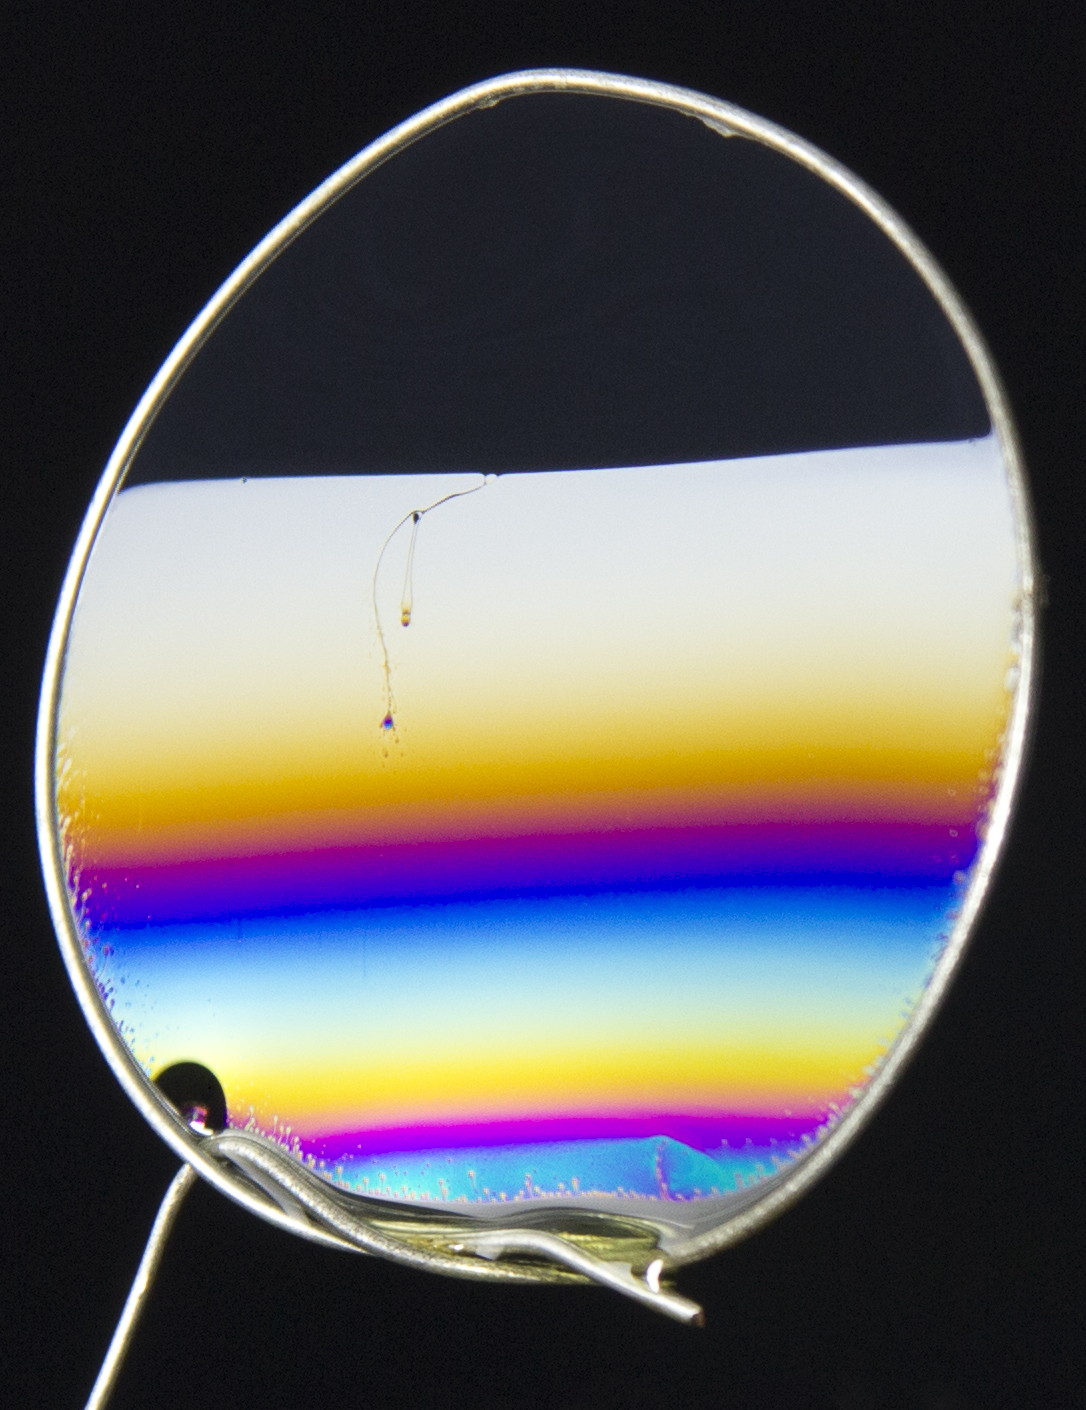
\includegraphics[scale=1]{soapfilm.jpg}
        \caption{A soap film showing destructive interference at the top due to a phase shift upon reflection and a spectrum lower down due to varying thickness. Image credit: \url{https://www.animations.physics.unsw.edu.au/jw/light/soap-bubbles.htm} accessed on 27/04/2021.}
        \label{fig:soap film}
    \end{figure}
    
    \subsection{Newton's Rings/Newton's Wedge}
    Newton's rings and Newton's wedge are related phenomena where a slowly increasing gap between two glass components causes a pattern of fringes, see figure~\ref{fig:newtons wedge and rings}.
    Newton's wedge uses two flat pieces of glass laid on top of each other with the upper piece being raised slightly on one side such that the gap between the two pieces is wedged shaped see figure~\ref{fig:newtons wedge}.
    Newton's rings uses a planar-convex of radius \(R\) with the lens placed convex side down on a flat glass surface so that moving away from the centre results in the space between the lens and the glass increases as you move away fro m the centre of the lens, see figure~\ref{fig:newtons rings}.
    The result of both of these is that incident light is split, ignoring second order reflections and reflections off of a glass-air boundary there will be two beams that leave the setup.
    
    For Newton's wedge the way that this works is the first beam reflects off of the first air-glass boundary and the second makes it through this boundary and into the small space between the two pieces of glass before reflecting off of the next air-glass boundary.
    Consider Newton's wedge and in particular pick two adjacent bright fringes along the wedge such that the size of the air gap is \(d_a\) at the first point and \(d_b\) at the second.
    The phase thickness is then \(\beta_a = 2\pi d_a/\lambda\) at the first point and \(\beta_b = 2\pi d_b/\lambda\) at the second.
    If the distance between the two points is \(\Delta x\) then simple geometry gives us
    \[\tan\alpha = \frac{d_b - d_a}{\Delta x} = \frac{\lambda}{2\Delta x} \implies \Delta x = \frac{\lambda}{2\tan\alpha} \approx \frac{\lambda}{2\alpha}.\]
    
    Consider now Newton's rings.
    In this case we have normal incidence on the top plane of the lens.
    The two beams that interact this time are the beam that reflects off of the convex face of the lens and the beam that reflects off the glass block below.
    At a distance \(r\) from the centre of the lens the thickness of the air gap is \(d\).
    Taking the convex side of the lens to be part of a sphere we have that
    \[(R - d)^2 + r^2 = R^2 \implies r^2 = 2Rd - d^2 \implies d \approx \frac{r^2}{2R}\]
    where the approximation assumes that \(d \ll R\).
    This equates to approximating the spherical lens face as parabolic.
    The phase shift between the two beams is twice the thickness of this air gap minus \(\pi\) due to the phase change upon reflection at the glass-air boundary.
    \[\delta = 2 \cdot 2\pi\frac{d}{\lambda} - \pi = \frac{2\pi r^2}{R\lambda} - \pi.\]
    We get bright fringes when \(\delta = 2m\pi\) for \(\pi\in\integers\) so bright fringes occur at distances
    \[r_m = \sqrt{\left( m + \frac{1}{2} \right)\lambda R}.\]
    Notice that at the centre, \(r = 0\), we get a dark fringe due to the fact that there is no boundary at the centre where the two glass components touch and therefore no reflection.
    \begin{figure}[htbp!]
        \centering
        \begin{subfigure}[b]{0.45\textwidth}
            \centering\tikzexternaldisable
            \tikzsetnextfilename{Newtons-wedge}
            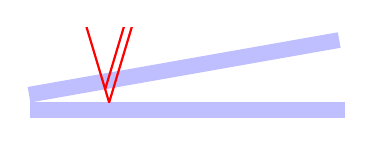
\begin{tikzpicture}
                \tikzset{glass/.style={blue!25}}
                \tikzset{light/.style={red, thick}}
                \fill[glass] (0, 0) rectangle (4, -0.2);
                \fill[glass, rotate=10] (0, 0) rectangle (4, 0.2);
                \begin{scope}
                    \clip (0, 0) rectangle (1.5, 0.95);
                    \draw[light] (0.7, 1) -- (1, 0) -- (1.3, 1);
                    \draw[light, xshift=-0.05cm, yshift=0.17cm] (1, 0) -- (1.3, 1);
                \end{scope}
            \end{tikzpicture}
            \caption{Newton's Wedge}
            \label{fig:newtons wedge}
        \end{subfigure}
        \begin{subfigure}[b]{0.45\textwidth}
            \centering
            \tikzsetnextfilename{Newtons-rings}
            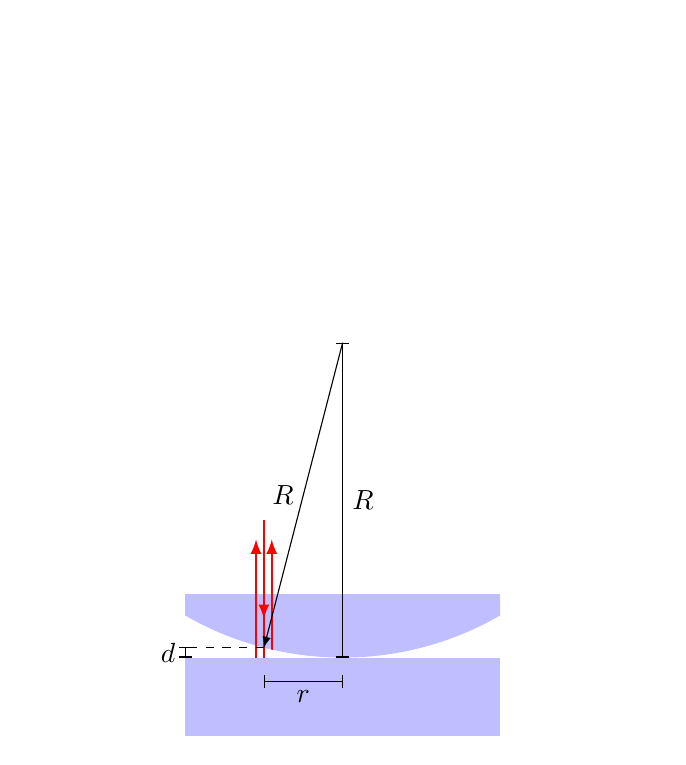
\begin{tikzpicture}
                \tikzset{glass/.style={blue!25}}
                \tikzset{light/.style={red, thick}}
                \fill[glass] (0, 0) rectangle (4, -1);
                \begin{scope}
                    \clip (0, 0) rectangle (4, 0.8);
                    \fill[glass] (2, 4) circle[radius=4];
                \end{scope}
                \draw[light] (1, 1.75) -- (1, 0);
                \draw[light, ->, >=latex] (1, 0.5) -- (1, 0.49);
                \begin{scope}
                    \clip (2, 4) circle[radius=4];
                    \draw[light, ->, >=latex] (1.1, 0) -- (1.1, 1.5);
                \end{scope}
                \draw[light, ->, >=latex] (0.9, 0) -- (0.9, 1.5);
                \draw[|-|] (1, -0.3) -- (2, -0.3) node[midway, below] {\(r\)};
                \draw[|-|] (2, 0) -- (2, 4) node[midway, right] {\(R\)};
                \draw[->, >=latex] (2, 4) -- (1, 0.125) node[midway, left] {\(R\)};
                \draw[dashed] (1, 0.125) -- (0, 0.125);
                \draw[|-|] (0, 0.13) -- (0, 0) node[midway, left] {\(d\)};
            \end{tikzpicture}
            \caption{Newton's Rings}
            \label{fig:newtons rings}
        \end{subfigure}
        \caption{Newton's Wedge and Newton's Rings create a series of bright and dark fringes through a similar mechanism of a gradually increasing air gap.}
        \label{fig:newtons wedge and rings}
    \end{figure}
    
    \subsection{Films to Increase/Decrease Reflectivity}
    By cleverly layering films it is possible to dramatically change the reflectivity of a material.
    The simplest example involves two layers of film onto glass, first a low refractive index layer and then a high refractive index layer.
    This way light has to pass from air to low, to high, to glass.
    Each time the light passes through one of these boundaries the refractive index is relatively higher and therefore the light that is reflected picks up a phase shift of \(\pi\).
    By constructing these layers to be the correct thickness it is possible to have destructive interference for the light that is reflected off of the different layers decreasing reflectivity and increasing transmissivity.
    
    Similarly a system of alternating low and high refractive index films can encourage many reflections which, if the thickness of the layers is correct, interfere constructively resulting in high reflectivity which allows us to make a mirror out of a transparent medium.
    
    \section{More Thin Film}
    \subsection{Non-Normal Incidence}
    Consider a bubble.
    When viewed at the right angle the bubble will appear multicoloured.
    This is due to thin film effects.
    The colours also change as the thickness of the bubble is not constant.
    More interestingly the colours also change based on the angle of viewing which is an effect known as \define{iridescence} which we will study in this section.
    
    \begin{figure}[ht]
        \centering
        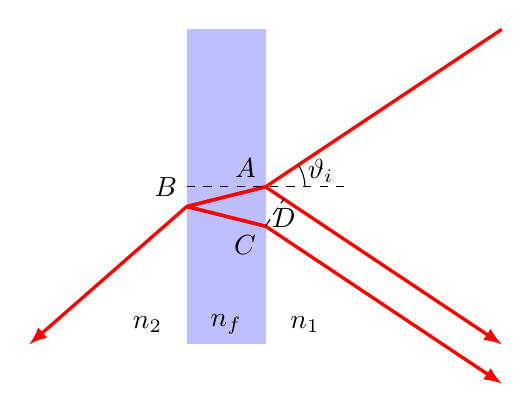
\begin{tikzpicture}
            \tikzset{film/.style={blue!25}}
            \tikzset{light/.style={red, very thick}}
            \fill[film] (0, 0) rectangle (1, 4);
            \begin{scope}
                \clip (1, 2) -- (4, 4) -- (2, 2) -- cycle;
                \draw (1, 2) circle[radius=0.5];
            \end{scope}
            \node at (1.7, 2.2) {\(\vartheta_i\)};
            \draw[light] (4, 4) -- (1, 2);
            \draw[light, ->, >=latex] (1, 2) -- (4, 0);
            \draw[light, ->, >=latex] (0, 1.75) -- (1, 1.5) -- (4, -0.5);
            \draw[light, ->, >=latex] (1, 2) -- (0, 1.75) -- (-2, 0);
            \begin{scope}
                \clip (0, 0) rectangle (1, 4);
                \draw[light] (1, 2) -- (0, 1.75) -- (1, 1.5);
            \end{scope}
            \draw[dashed] (0, 2) -- (2, 2);
            \draw[densely dashed] (1, 1.5) -- (1.23077, 1.84615);
            \node[above left] at (1, 2) {\(A\)};
            \node[above left] at (0, 1.75) {\(B\)};
            \node[below left] at (1, 1.5) {\(C\)};
            \node[below] at (1.23077, 1.84615) {\(D\)};
            \node at (1.5, 0.25) {\(n_1\)};
            \node at (0.5, 0.25) {\(n_f\)};
            \node at (-0.5, 0.25) {\(n_2\)};
        \end{tikzpicture}
        \caption{Thin film viewed at non-normal incidence.}
        \label{fig:thin film non-normal incidence}
    \end{figure}
    
    Consider the setup in figure~\ref{fig:thin film non-normal incidence}, a thin transparent film of thickness \(d\) and refractive index \(n_f\) separating two media of refractive indices \(n_1\) and \(n_2\).
    Over a small region we can approximate the sides of the film as parallel.
    Illuminate this film with a monochromatic point source.
    Since the film is transparent we will ignore secondary reflections.
    Since we are no longer restricting ourselves to normal incidence the optical path difference between a ray that reflects of of the medium one-film boundary and a ray that reflects of of the film-medium two boundary now depends on the angle at which the ray travels through the film, which is the transition angle.
    In fact the optical path difference is \(2n_f d/\cos\vartheta_t - n_1AD\) which is the optical path length that the second ray travels through the film while the first ray travels the optical length \(AD\).
    For simplicity we take \(n_1 = n_2\) and we find that the phase difference between the two rays is
    \begin{align*}
        \delta &= \frac{2\pi}{\lambda_{\mathrm{vac}}} \left[ \frac{2n_f}{cos
        \vartheta_t} - n_1AD \right] - \pi\\
        &= \frac{2\pi}{\lambda_{\mathrm{vac}}} \left[ \frac{2n_fd}{\cos\vartheta_t} - n_1AC\sin\vartheta_1 \right] - \pi\\
        &= \frac{2\pi}{\lambda_{\mathrm{vac}}} \left[ \frac{2n_fd}{\cos\vartheta_t} - n_1AC\sin\vartheta_t\frac{n_f}{n_i} \right] - \pi\\
        &= \frac{2\pi}{\lambda_{\mathrm{vac}}} \left[ \frac{2n_fd}{\cos\vartheta_t} - n_fAC\sin\vartheta_t \right] - \pi.
    \end{align*}
    Here we've used Snell's law to get all angles in terms of \(\vartheta_t\) and we've included a phase shift of \(\pi\) since exactly one of the reflections is off of a higher refractive index medium.
    A final bit of geometry tells us that \(AC = 2d\tan\vartheta_t\) and so
    \[\delta = \frac{4\pi n_f}{\lambda_{\mathrm{vac}}}d\cos\vartheta_t - \pi.\]
    So there is constructive interference if
    \[d\cos\vartheta_t = (2m - 1)\frac{\lambda_f}{4}\]
    for some \(m\in\integers\).
    Similarly there is destructive interference if
    \[d\cos\vartheta_t = 2m\frac{\lambda_f}{4}.\]
    We can see that in the case of normal incidence we have \(\vartheta_i = \vartheta_t = 0\) and so this reduces to the same relationship that we have for film thickness at normal incidence.
    
    \subsubsection{White Light Illumination}
    We can use Snell's law to write the results of the last section in terms of \(\vartheta_i\):
    \[d_{\mathrm{constructive}} = \frac{(2m - 1)\lambda_{\mathrm{vac}}}{4\sqrt{n_f^2 - n_i^2\sin^2\vartheta_i}}, \qquad\text{and}\qquad d_{\mathrm{destructive}} = \frac{2m\lambda_{\mathrm{vac}}}{4\sqrt{n_f^2 - n_i^2\sin^2\vartheta_i}}.\]
    This makes the connection between viewing angle and interference more explicit.
    Since this also depends on wavelength we see that if we illuminate the film with a white source then at different viewing angles we will see different colours.
    
    This effect is common in nature.
    It is seen in bird's feathers and seashells, which are formed of many thin layers, as well as in bismuth crystals which quickly builds up a film of oxidised bismuth.
    
    \begin{figure}[htb]
        \begin{subfigure}[t]{0.2\textwidth}
            \centering
            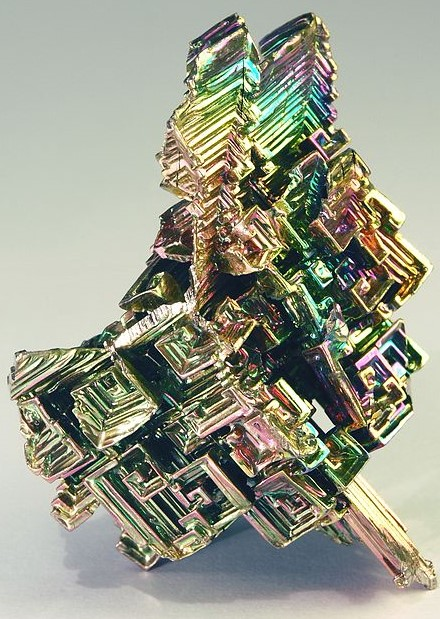
\includegraphics[height=3.5cm]{bismuth.jpg}
            \caption{Bismuth. Image credit: \copyright{}Micha L. Rieser {\scriptsize \url{https://commons.wikimedia.org/wiki/File:Bismuth-crystal.jpg}.}}
        \end{subfigure}
        \begin{subfigure}[t]{0.4\textwidth}
            \centering
            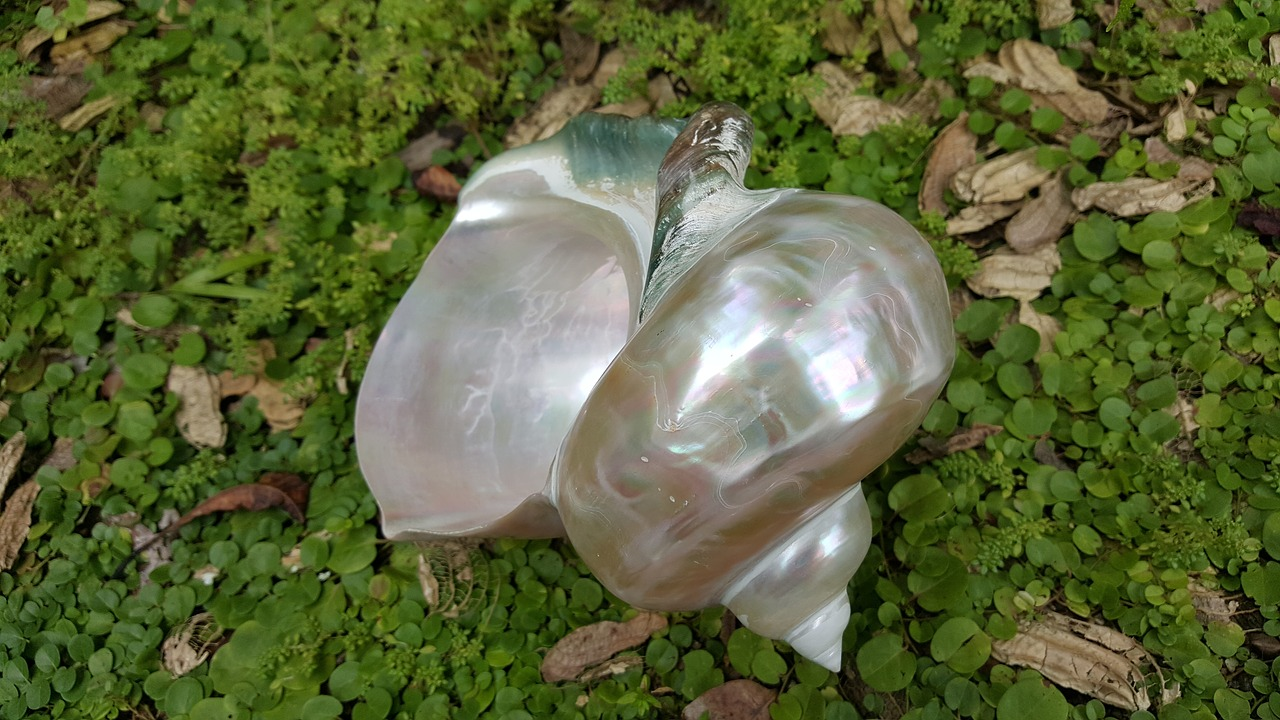
\includegraphics[height=3.5cm]{shell.jpg}
            \caption{Shell. Image credit: {\scriptsize \url{https://pixabay.com/photos/pearl-fire-oud-shells-nautilus-sea-1602541/}.}}
        \end{subfigure}
        \begin{subfigure}[t]{0.3\textwidth}
            \centering
            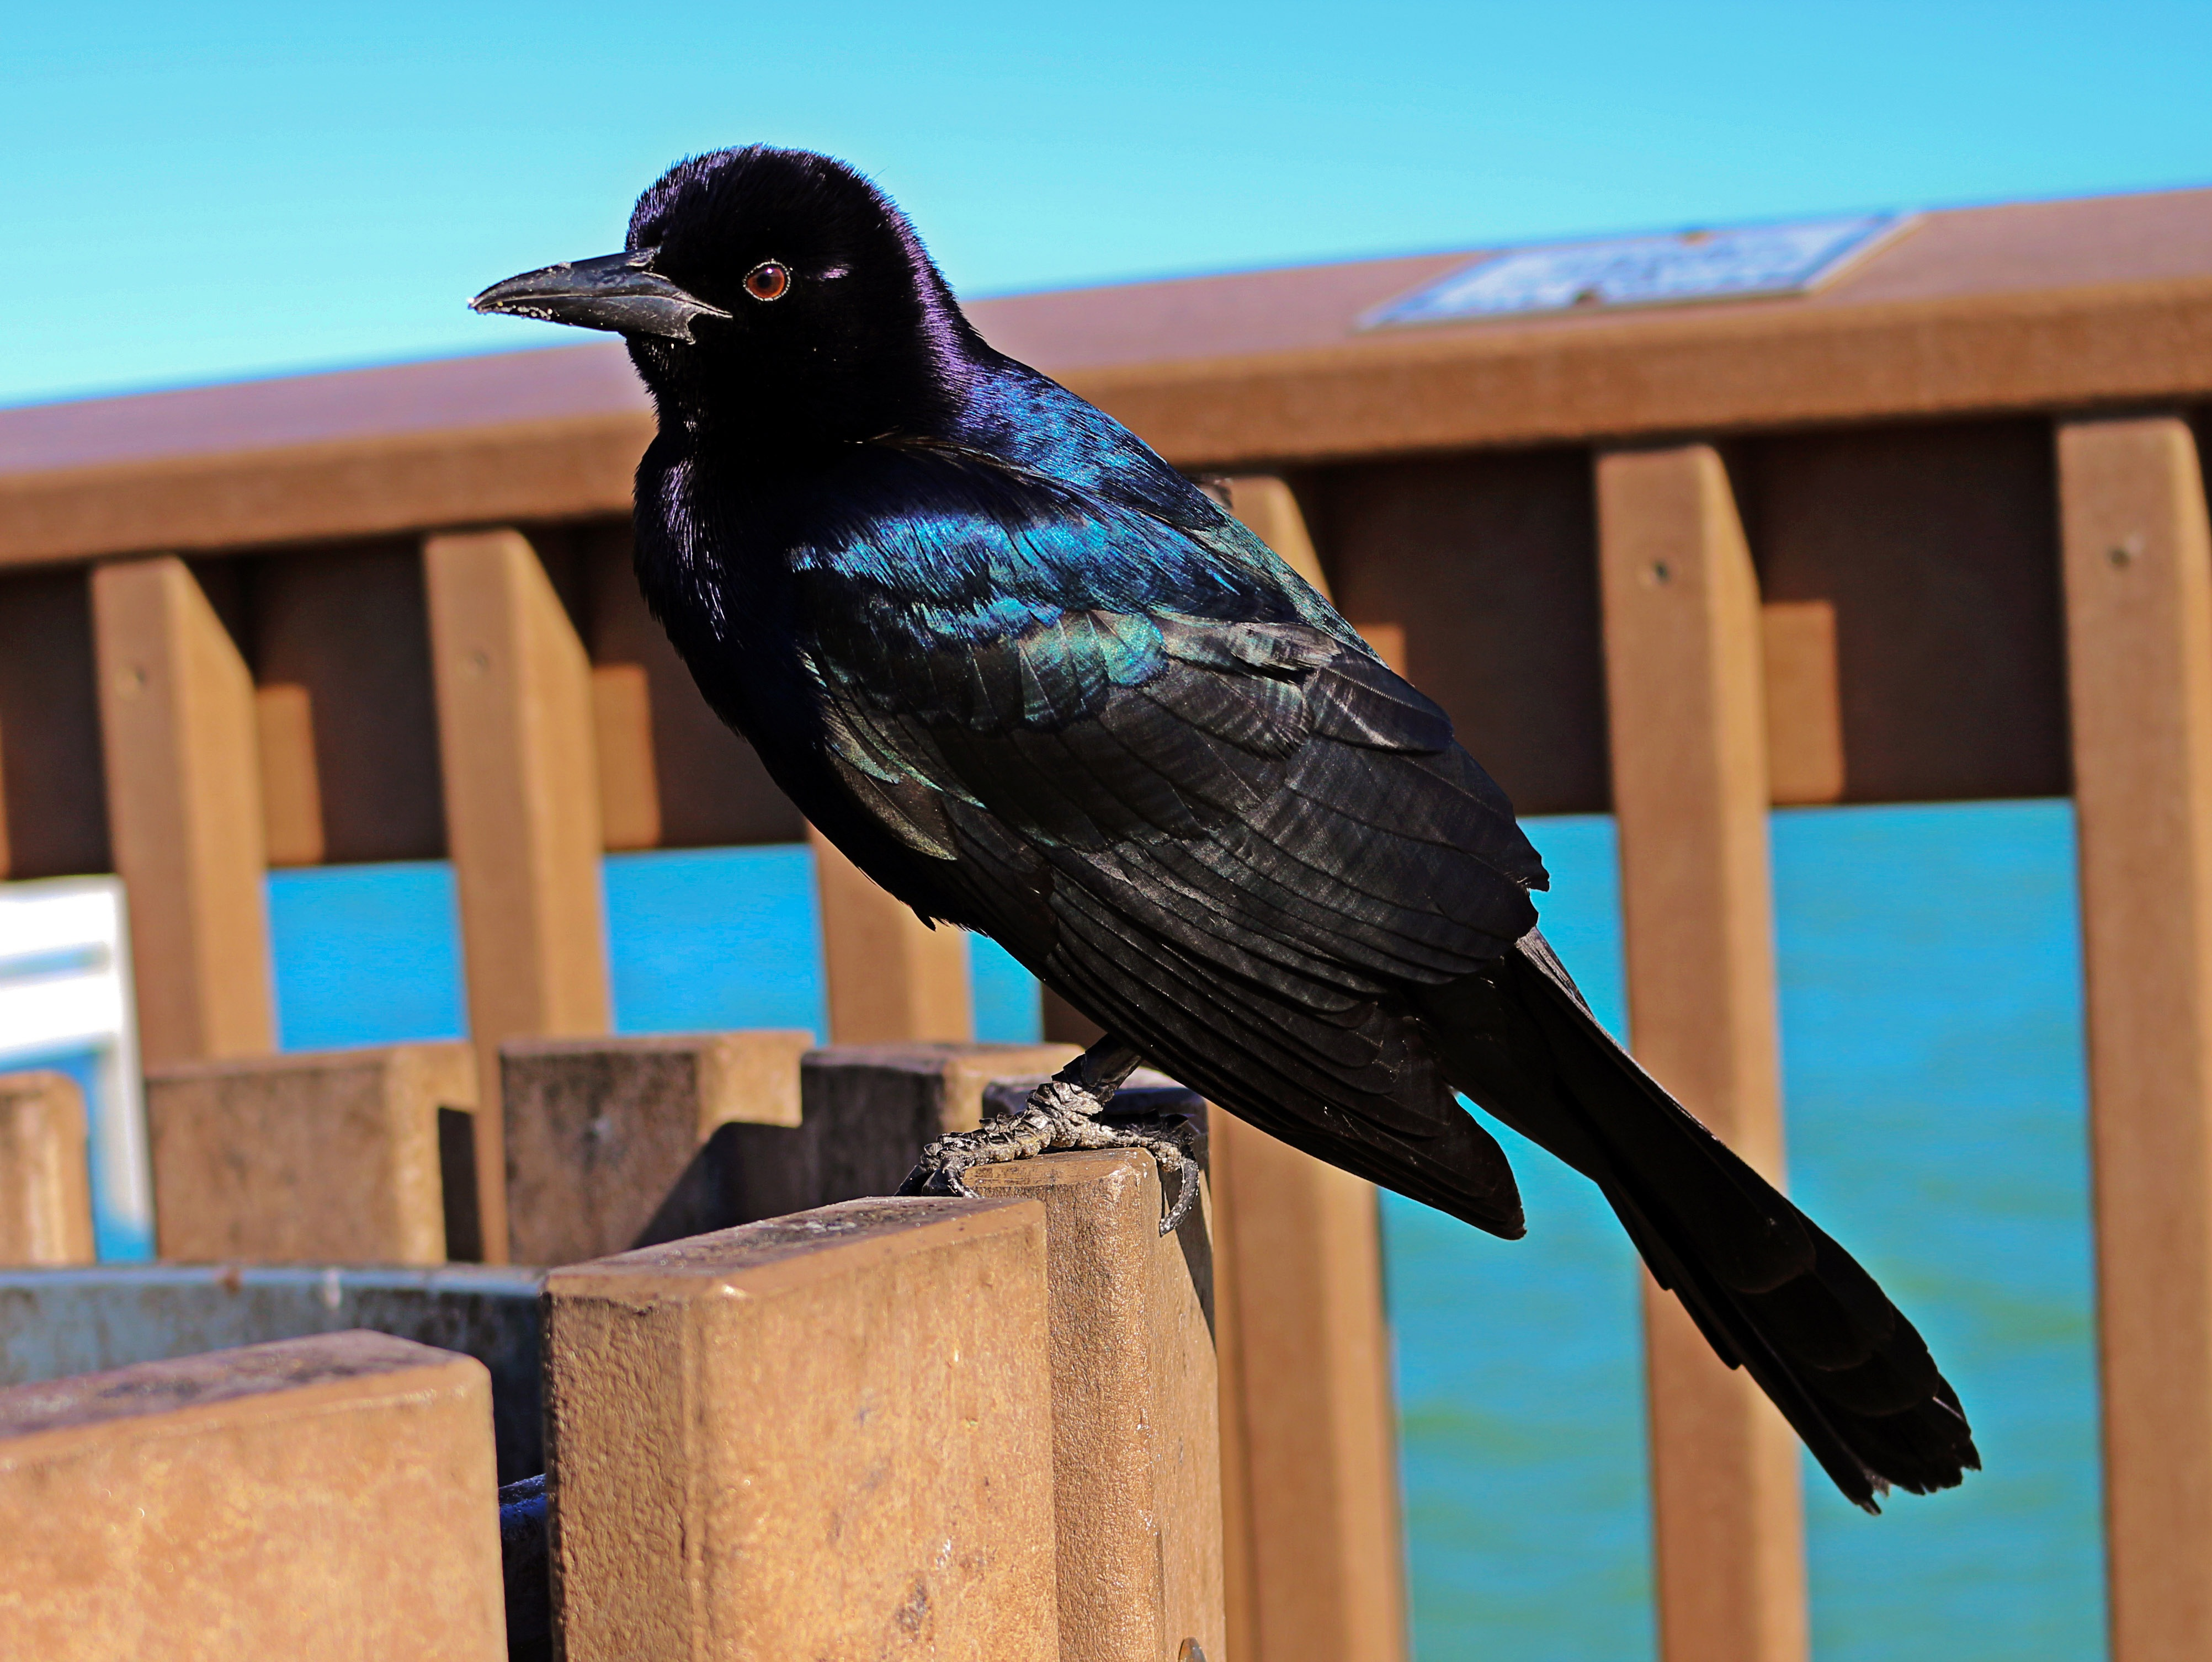
\includegraphics[height=3.5cm]{bird.jpg}
            \caption{Bird. Image credit: {\scriptsize \url{https://pxhere.com/en/photo/653981}.}}
        \end{subfigure}
        \caption{Some natural examples of thin films causing iridescence.}
    \end{figure}

    \subsection{Multiple Reflections}
    Up to now we have assumed that all secondary reflections are sufficiently weak that they can be ignored.
    This isn't the case for a non-transparent material and is only an approximation for a transparent material.
    
    Consider an air-film-glass setup.
    The first reflection off of the air-film boundary has reflection coefficient \(r_1 = r_{af}\).
    The second reflection is off of the film-glass boundary and has reflection coefficient 
    \[r_2 = t_{af}e^{i\beta}r_{fg}e^{i\beta}t_{fa}.\]
    The factor of \(t_{af}\) accounts for the fact that this ray is first transmitted at the air-film boundary.
    It then travels through the medium picking up a phase factor of \(e^{i\beta}\) (\(\beta = 2\pi n_fd\cos\vartheta_t/\lambda\)).
    It is then reflected at the film-glass boundary picking up a factor of \(r_{fg}\), travels back through the film picking up another \(e^{i\beta}\) and finally is transmitted at the film-air boundary picking up a factor of \(t_{fa}\).
    The third reflection follows almost the same path but instead of being transmitted at the film-air boundary it is reflected \((r_{fa})\), travels back through the film \((e^{i\beta})\), is reflected at the film-glass boundary \((r_{fg})\), travels back through the film, \((e^{i\beta})\), and is finally transmitted at the film-air boundary \((t_{fa})\).
    So the third ray to leave the film into the air has reflection coefficient
    \begin{align*}
        r_3 &= t_{af}e^{i\beta}r_{fg}e^{i\beta}(r_{fa}e^{i\beta}r_{fg}e^{i\beta})t_{fa}\\
        &= r_2(r_{fa}e^{2i\beta}r_{fg}).
    \end{align*}
    By the same logic we can write the reflection coefficient for the fourth reflected ray as
    \[r_{4} = r_3x = r_2x^2, \qquad\text{where}\qquad x = f_{fa}e^{2i\beta}r_{fg}.\]
    Continuing \textit{ad infinitum} we see that the total reflection coefficient is
    \[r_{afg} = r_1 + r_2(1 + x + x^2 + \dotsb) = r_1 + \frac{r_2}{1 - x}.\]
    In the last step we have identified the geometric series which converges if and only if \(\abs{x} < 1\).
    It can be shown then that
    \[f_{afg} = \frac{r_{af} + r_{fg}e^{2i\beta}}{1 + r_{af}}r_{fg}e^{2i\beta}.\]
    
    Suppose we have an unsupported thin film, that is the film has the same medium on either side (as opposed to being layered onto glass).
    For simplicity we will also assume that this medium is air.
    Then
    \[f_{afa} = \frac{r_{af} + r_{fa}e^{2i\beta}}{1 + r_{af}r_{fa}e^{2i\beta}} = \frac{r_{af} - r_{af}e^{2i\beta}}{1 - r_{af}r_{af}e^{2i\beta}} = \frac{r[1 - e^{2i\beta}]}{1 - r^2e^{2-\beta}}\]
    where we right \(r = r_{af}\) for brevity.
    The reflectivity of the film is then
    \begin{align*}
        R &= \abs{r_{afa}}^2\\
        &= \frac{r[1 - e^{2i\beta}]}{1 - r^2e^{2i\beta}}\frac{r[1 - e^{-2i\beta}]}{1 - r^2e^{-2i\beta}}\\
        &= \frac{2r^2[1 - \cos(2\beta)]}{1 - 2r^2\cos(2\beta) + r^4}.
    \end{align*}
    We assumed here that \(r\in\reals\) which means that \(n\in\reals\) which means that we are considering only transparent, non-absorbing, materials.
    We then have that the transmissivity is
    \[T = 1 - R = \frac{(1 - r)^2}{1 - 2r^2\cos(2\beta) + r^4}.\]
    This is minimised when \(\cos(2\beta) = -1\) so \(4\pi n_fd\cos\vartheta_t/\lambda = (2m - 1)\pi\) for \(m\in\integers\).
    We find that
    \[\min\{T\} = \frac{(1 - r^2)^2}{(1 + r^2)^2}\]
    and
    \[\max\{R\} = 1 - \min\{T\} = \frac{4r^2}{(1 + r^2)^2}.\]
    We can introduce the \define{Finesse coefficient}, \(F\), here defined as
    \[F = \left( \frac{2r}{1 - r^2} \right)^2\]
    which allows us to write
    \[R = \frac{F\sin^2\beta}{1 + F\sin^2\beta}, \qquad\text{and}\qquad T = \frac{1}{1 + F\sin^2\beta}.\]
    For small \(r\) we have an approximately \(\sin^2\) fringe pattern, just as we observed for two beam interference.
    For larger values of \(r\) however we have strong multiple reflections and a more complex fringe pattern.
    As \(r \to 1\) we have \(T \to 0\) and \(R \to 1\) unless \(\beta = m\pi\) for some \(m\in\integers\) in which case we have narrow bands which appear bright viewing with the source on the other side of the film or as dark viewing on the same side as the source.
    \(R\) and \(T\) plotted for various values of \(r\), \(F\), and \(\beta\) can be seen in figure~\ref{fig:reflectivity and transmissivity}.
    
    \begin{figure}[htbp!]
        \centering
        \begin{subfigure}{0.9\textwidth}
            \centering
            \tikzsetnextfilename{thin-film-reflectivity}
            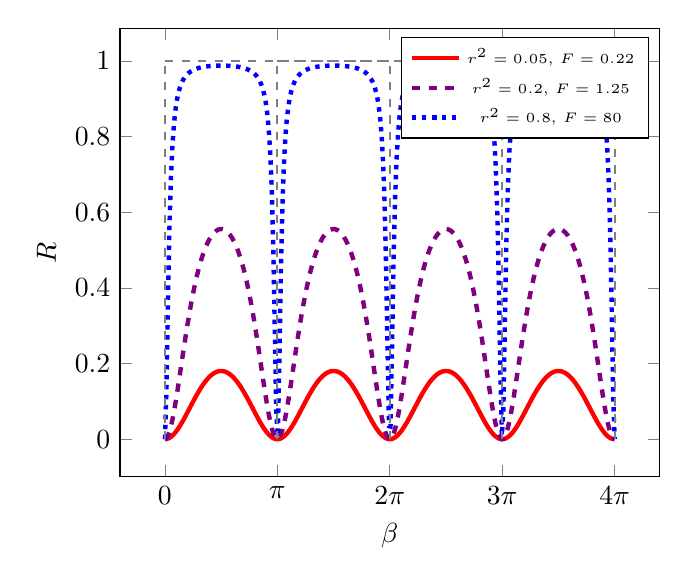
\begin{tikzpicture}
                \tikzset{myplot/.style={ultra thick}}
                \begin{axis}[
                    domain=0:4*pi,
                    xlabel=\(\beta\),
                    ylabel=\(R\),
                    xtick={
                        0, pi, 2*pi, 3*pi, 4*pi
                    },
                    xticklabels={
                        0, \(\pi\), \(2\pi\), \(3\pi\), \(4\pi\)
                    },
                    samples=300
                    ]
                    % Plots
                    \addplot[
                    myplot,
                    red
                    ] {1 - 1 / (1 + 0.22 * sin(deg(x))^2)};  % r^2 = 0.05, F= 0.22
                    \addplot[
                    myplot,
                    red!50!blue,
                    dashed
                    ] {1 - 1 / (1 + 1.25 * sin(deg(x))^2)};  % r^2 = 0.2, F = 1.25
                    \addplot[
                    myplot,
                    blue,
                    dotted
                    ] {1 - 1 / (1 + 80 * sin(deg(x))^2)};  % r^2 = 0.8, F = 80
                    
                    % Guide lines
                    \draw[dashed, thick, gray] (0, 1) -- (4*pi, 1);
                    \draw[dashed, thick, gray] (pi, 1) -- (4*pi, 1);
                    \draw[dashed, thick, gray] (0, 0) -- (0, 1);
                    \draw[dashed, thick, gray] (pi, 0) -- (pi, 1);
                    \draw[dashed, thick, gray] (2*pi, 0) -- (2*pi, 1);
                    \draw[dashed, thick, gray] (3*pi, 0) -- (3*pi, 1);
                    \draw[dashed, thick, gray] (4*pi, 0) -- (4*pi, 1);
                    
                    % Legend
                    \addlegendentry{\tiny\(r^2 = 0.05\), \(F = 0.22\)}
                    \addlegendentry{\tiny\(r^2 = 0.2\), \(F = 1.25\)}
                    \addlegendentry{\tiny\(r^2 = 0.8\), \(F = 80\)}
                \end{axis}
            \end{tikzpicture}
            \caption{The reflectivity, \(R\).}
        \end{subfigure}
        \begin{subfigure}{0.9\textwidth}
            \centering
            \tikzsetnextfilename{thin-film-transmissivity}
            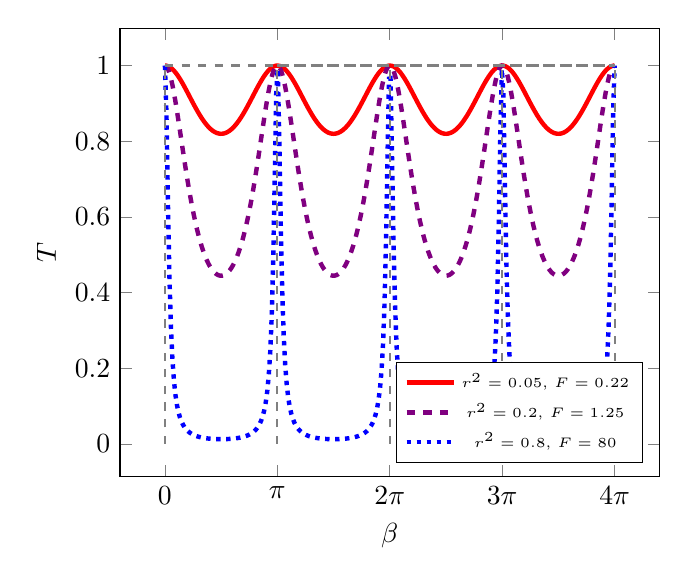
\begin{tikzpicture}
                \tikzset{myplot/.style={ultra thick}}
                \begin{axis}[
                    domain=0:4*pi,
                    xlabel=\(\beta\),
                    ylabel=\(T\),
                    xtick={
                        0, pi, 2*pi, 3*pi, 4*pi
                    },
                    xticklabels={
                        0, \(\pi\), \(2\pi\), \(3\pi\), \(4\pi\)
                    },
                    samples=300,
                    legend pos=south east
                    ]
                    % Plots
                    \addplot[
                    myplot,
                    red
                    ] {1 / (1 + 0.22 * sin(deg(x))^2)};  % r^2 = 0.05, F= 0.22
                    \addplot[
                    myplot,
                    red!50!blue,
                    dashed
                    ] {1 / (1 + 1.25 * sin(deg(x))^2)};  % r^2 = 0.2, F = 1.25
                    \addplot[
                    myplot,
                    blue,
                    dotted
                    ] {1 / (1 + 80 * sin(deg(x))^2)};  % r^2 = 0.8, F = 80
                    
                    % Guide lines
                    \draw[dashed, thick, gray] (0, 1) -- (4*pi, 1);
                    \draw[dashed, thick, gray] (pi, 1) -- (4*pi, 1);
                    \draw[dashed, thick, gray] (0, 0) -- (0, 1);
                    \draw[dashed, thick, gray] (pi, 0) -- (pi, 1);
                    \draw[dashed, thick, gray] (2*pi, 0) -- (2*pi, 1);
                    \draw[dashed, thick, gray] (3*pi, 0) -- (3*pi, 1);
                    \draw[dashed, thick, gray] (4*pi, 0) -- (4*pi, 1);
                    
                    % Legend
                    \addlegendentry{\tiny\(r^2 = 0.05\), \(F = 0.22\)}
                    \addlegendentry{\tiny\(r^2 = 0.2\), \(F = 1.25\)}
                    \addlegendentry{\tiny\(r^2 = 0.8\), \(F = 80\)}
                \end{axis}
            \end{tikzpicture}
            \caption{The transmissivity, \(T\).}
        \end{subfigure}
        \caption{The reflectivity and transmissivity, \(R\) and \(T\), for an unsupported thin film in air.}
        \label{fig:reflectivity and transmissivity}
    \end{figure}
    
    For high values of \(r\) or \(F\) the transmissivity is very selective for specific values of \(\beta\), and hence for specific wavelengths.
    This is exploited in \define{Fabry-Perot} systems which are comprised of two parallel highly reflective surfaces, usually dielectric mirrors made with multiple layers of thin films.
    The two mirrors are separated by a distance \(d\) and filled with a medium of refractive index \(n\).
    If the cavity is then illuminated by a collimated beam (that is light where all rays are parallel) of amplitude \(E_0\) which enters at angle \(\vartheta_0\) to the normals of the mirrors.
    If we choose \(\vartheta_0 = 0\) then we will get transmission of wavelengths close to
    \[\lambda_m = \frac{2nd}{m}\]
    where \(m\in\integers\).
    This corresponds to a half-integer number of wavelengths fitting in the cavity.
    The result is that only light within a very narrow range around these key values of \(\lambda_m\) can pass out of the cavity so it acts as a very narrow bandpass filter.
    \endgroup
    
    \part{Diffraction}
    \section{Basic Diffraction}
    So far we have considered only homogenous media and abrupt boundaries.
    If we need to study inhomogeneous media then we need the idea of diffraction.
    This is the process by which light is partially blocked and how the light propagates past the blockage.
    We will consider a scalar wave model in this section, which means we will ignore polarisation effects and consider only the amplitude of the wave.
    We are mostly interested in the intensity, \(I = cn\varepsilon_0E_0^2/2\).
    However we only really care about relative intensity, which points will be dark and which will be light, so we will often drop the prefactor and take \(I = E_0^2\).
    
    \subsection{The Huygens--Fresnel Principle}
    Huygens' principle was discussed in section~\ref{sec:huygens principle}.
    This same principle can be adapted to explain diffraction.
    One of the problems with Huygens' principle is that it treats all waves the same, regardless of wavelength, which doesn't match reality.
    For example it is possible to hear something that is happening around the corner but not see it.
    For some reason the sound waves are able to bend around the corner in a way that light cannot.
    We also ignored the backwards propagating wavelets when we first considered Huygens' principle and we only drew the wavelets necessary to create the next wavefront.
    
    Fresnel proposed a correction to Huygens' principle that interference of secondary wavelets was what lead to only the forward propagation being important.
    The amended \define{Huygen--Fresnel principle} can be stated as:
    \begin{displayquote}
        Every unobstructed point of a wavefront serves as a source of spherical secondary wavelets having the same frequency and speed as the primary wave. The resulting optical disturbance is given by the superposition of all the secondary waves.
    \end{displayquote}
    This seems like a fairly superficial change initially, we've simply included the fact that the secondary wavelets are waves and therefore interfere with each other.
    However, this manages to fix a lot of the problems with Huygens' principle.
    
    \subsubsection{Single Slit Diffraction}
    \begin{figure}[htb]
        \centering
        \tikzsetnextfilename{single-slit-diffraction}
        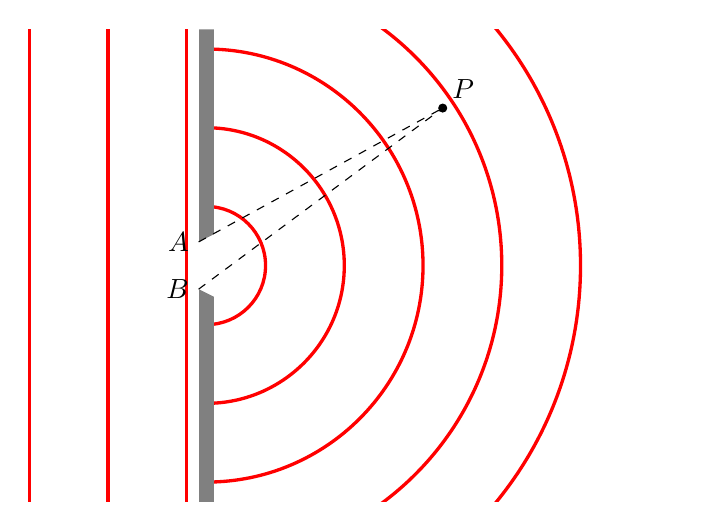
\begin{tikzpicture}
            \tikzset{boundary/.style={gray, line width=0.2cm}}
            \tikzset{wavefront/.style={red, very thick}}
            \foreach \x in {-0.25, -1.25, -2.25} {
                \draw[wavefront] (\x, -3) -- (\x, 3);
            }
            \begin{scope}
                \clip (0, -3) rectangle (6, 3);
                \foreach \r in {0.75, 1.75, 2.75, 3.75, 4.75} {
                    \draw[wavefront] (0, 0) circle[radius=\r];
                }
            \end{scope}
            \begin{scope}
                \clip (-0.1, -0.3) -- (0.1, -0.4) -- (0.1, -3) -- (-0.1, -3) -- cycle;
                \draw[boundary] (0, -3) -- (0, -0.3);
            \end{scope}
            \begin{scope}
                \clip (-0.1, 0.3) -- (0.1, 0.4) -- (0.1, 3) -- (-0.1, 3) -- cycle;
                \draw[boundary] (0, 3) -- (0, 0.3);
            \end{scope}
            \coordinate (P) at (3, 2);
            \draw[fill=black] (P) circle[radius=0.05cm] node[above right] {\(P\)};
            \draw[dashed] (-0.1, 0.3) -- (P);
            \draw[dashed] (-0.1, -0.3) -- (P);
            \node[left] at (-0.1, 0.3) {\(A\)};
            \node[left] at (-0.1, -0.3) {\(B\)};
        \end{tikzpicture}
        \caption{Single slit diffraction.}
        \label{fig:single slit diffraction}
    \end{figure}
    Consider a single slit of width \(a = AB\), as shown in figure~\ref{fig:single slit diffraction}.
    At a given point, \(P\), the maximum possible optical path difference (assuming the wave propagates through air so \(n = 1\) for simplicity) is \(\ell = \abs{BP - AP}\).
    This is at most equal to the slit width, \(a = AB\).
    If the wavelength of the light, \(\lambda \gg a\) then we also have \(\lambda \gg \ell\).
    Since all secondary wavelets at the slit are in phase we will then have constructive interference at \(P\).
    This makes no assumption about where \(P\) is so for a narrow slit (narrow being defined as \(\lambda \gg a\)) we have constructive interference everywhere.
    
    If instead \(\lambda \ll a\) then we only have \(\lambda \gg \ell\) if \(\ell\) happens to be particularly small.
    This only occurs just in front of the slit, and slightly off to the side.
    Above a certain angle we will have \(\ell \approx \lambda\) and we will have destructive interference.
    What we have discovered here is we can only have geometrically perfect shadows, with sharp edges, in the limit \(\lambda/a\to 0\).
    
    \subsection{Near and Far Field Diffraction}
    Consider a point source of wavelength \(\lambda\) placed at the origin.
    If we ignore the time varying part of the waves then the scalar amplitude at a point \(\vv{r}\) 
    \[E(\vv{r}) = \frac{\mathcal{A}}{r}\cos(kr)\]
    where \(k = 2\pi/\lambda\).
    Close to the point source we have to use this full equation and treat the waves as spherical.
    
    Notice that we can write \(r\) as
    \[r = \sqrt{x^2 + y^2 + z^2} = z\sqrt{\frac{x^2 + y^2}{z^2} + 1} = z\left( 1 + \frac{x^2 + y^2}{z^2} \right).\]
    If we consider the waves at some point with \(z \gg x, y\) then using the binomial expansion we have
    \[r \approx z + \frac{x^2 + y^2}{2z}.\]
    This corresponds to assuming that the wave fronts are locally parabolic.
    We call this the Fresnel or near field diffraction regime.
    
    Even further from the origin we can approximate the waves as locally plane waves.
    At a distance \(D\) from the point source at an angle \(\vartheta_0\) to the \(z\)-axis considering the point with \(y = y_0\) we have
    \[r\approx \frac{D}{\cos\vartheta_0} + (y - y_0)\sin\vartheta_0\]
    where \(y_0 = D\tan\vartheta_0\).
    See figure~\ref{fig:spherical waves approx plane waves}.
    We call this the Fraunhofer or far field regime.
    This is the regime in which we will work.
    \begin{figure}[htb]
        \centering
        \tikzsetnextfilename{plane-wave-approx}
        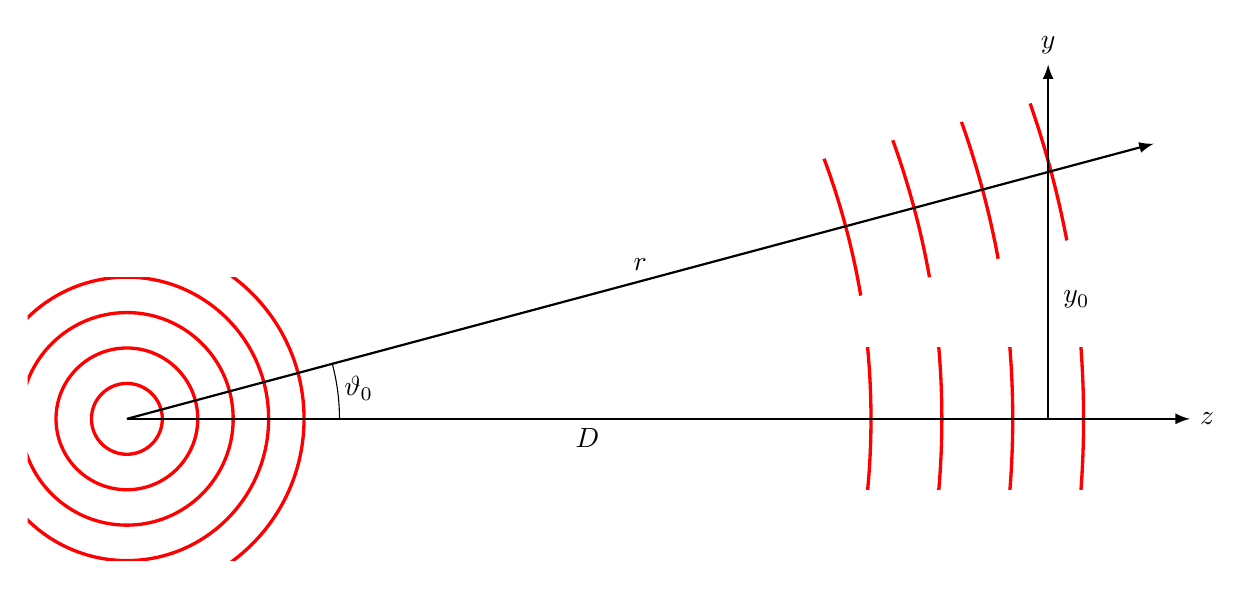
\begin{tikzpicture}[scale=0.9]
            \tikzset{wavefront/.style={red, very thick}}
            \begin{scope}
                \clip (-1.4, -2) rectangle (3, 2);
                \foreach \r in {0, 0.5,..., 2.5} {
                    \draw[wavefront] (0, 0) circle[radius=\r];
                }
            \end{scope}
            \begin{scope}
                \clip (10, -1) rectangle (14, 1);
                \foreach \r in {10.5, ..., 13.5} {
                    \draw[wavefront] (0, 0) circle[radius=\r];
                }
            \end{scope}
            \begin{scope}[rotate=15]
                \clip (10, -1) rectangle (14, 1);
                \foreach \r in {10.5, ..., 13.5} {
                    \draw[wavefront] (0, 0) circle[radius=\r];
                }
            \end{scope}
            \draw[->, >=latex, thick] (0, 0) -- (15, 0) node[right] {\(z\)};
            \draw[->, >=latex, thick] (0, 0) -- (15:15) node[midway, above] {\(r\)};
            \begin{scope}
                \clip (0, 0) -- (15, 0) -- (15:15) -- cycle;
                \draw (0, 0) circle[radius=3];
                \node at (7.5:3.3) {\(\vartheta_0\)};
            \end{scope}
            \draw[->, >=latex, thick] (13, 0) -- (13, 5) node[above] {\(y\)};
            \node[right] at ($(13, 0)!0.5!(15:13) + (0.3, 0)$) {\(y_0\)};
            \node[below] at (6.5, 0) {\(D\)};
        \end{tikzpicture}
        \caption{Far from the origin we can approximate spherical waves as plane waves.}
        \label{fig:spherical waves approx plane waves}
    \end{figure}
    
    \section{Single Slit Diffraction}
    \subsection{Far Field Single Slit Diffraction}
    Consider a single slit, \(a\), in the plane \(P_0\) being illuminated by a wave of wavelength \(\lambda\).
    We assume the slit is infinite in the other direction and take this direction to be the \(x\)-axis.
    We take the \(z\) axis to be normal to the plane.
    Consider a point \(s\) on the plane \(P_1\) which is at a distance \(D\) from the split and parallel to \(P_0\).
    The line from the middle of the slit to \(s\) makes an angle \(\vartheta\) to the \(z\) axis.
    We place the origin in the middle of the slit.
    As before we consider the two rays coming from \(A\) and \(B\), the edges of the slit, and in the far field approximation we consider these two rays to be parallel.
    
    Before we attempt a full solution we will consider what we expect.
    Suppose we split the slit into \(2n\) sections (here \(n\in\naturals\) is \emph{not} the refractive index), each of width \(a/2n\).
    Consider the path difference, \(\ell\), for a secondary wavelet reaching \(s\) from the upper edge of the slit and from a secondary wavelet reaching \(s\) from a point \(a/2n\) below that.
    Simple geometry gives us \(\ell = (a/2n)\sin\vartheta\).
    If \(s\) is such that \(\ell = \lambda/2\) then we will have destructive interference.
    In fact any point in the first segment will undergo destructive interference, not just the end point.
    The same logic applies for the next segment over and so we have the condition for minima:
    \[a\sin\vartheta = n\lambda, \qquad\text{for}\qquad n = 0, 1, 2, \dotsc.\]
    By symmetry the same applies for negative \(\vartheta\).
    
    If instead \(s\) lies on the \(z\)-axis then \(\vartheta = 0\) and all secondary wavelets arrive in phase causing a central maximum.
    This maximum is between two minima at \(\sin\vartheta = \pm \lambda/a\) and so the width is \(2\lambda/a\).
    We will also find maxima between the other neighbouring minima but the exact angle at which we find them is not simple to derive, however we do know that their widths are \(\lambda/a\).
    Notice the reciprocal relationship between slit width and peak width.
    We will see this again later.
    
    \subsubsection{Analytical Solution}
    We considered special cases of rays in the previous argument.
    Here we aim to develop a theory that works for all rays coming from the slit.
    To do this we have to account for the phase shifts of all secondary wavelets that arrive at the point \(s\).
    The optical path length of a ray leaving the slit at \(y\) is \(\ell = \ell_0 + y\sin\vartheta\) where \(\ell_0\) is the optical path length of travelled by light leaving the centre of the slit, however, for our purposes we can simply treat \(\ell_0\) as a constant as it just depends upon how far away we place the screen.
    The phase shift due to the point at which the light leaves the slit is then
    \[\delta(y) = 2\pi\frac{\ell(y)}{\lambda} = 2\pi\frac{y}{\lambda}\sin\vartheta.\]
    We can approximate the distance of \(s\) from the slit to be \(R = D/\cos\vartheta\) if \(D\) is large.
    We find that the total amplitude, ignoring oscillations, is then given by the superposition of the amplitudes of all rays arriving from anywhere on the slit:
    \begin{equation}\label{eqn:single slit amplitude}
        E(\vartheta) = \frac{\mathcal{A}}{R} = \int_{-a/2}^{a/2}\cos\delta \dd{y} = \frac{\mathcal{A}}{R}\int_{-a/2}^{a/2} \cos\left( 2\pi\frac{y}{\lambda}\sin\vartheta \right)\dd{y} = \frac{a\mathcal{A}}{R}\frac{\sin\beta}{\beta} = \frac{a\mathcal{A}}{R}\sinc\beta
    \end{equation}
    where \(\beta = (\pi a/\lambda)\sin\vartheta\).
    The intensity is then
    \[I(\vartheta) = \varepsilon v\expected{E^2} = \frac{\varepsilon v}{2}\left( \frac{a\mathcal{A}}{R} \right)^2\sinc^2\beta = I(0)\sinc^2\beta.\]
    This vanishes for \(\beta = n\pi\) where \(n\in\integers\setminus\{0\}\).
    This condition can also be written as \(a\sin\vartheta = n\lambda\), which agrees with our first attempt.
    See figure~\ref{fig:sinc squared} for a plot of the intensity.
    
    \begin{figure}[htb]
        \centering
        \tikzsetnextfilename{sinc-squared}
        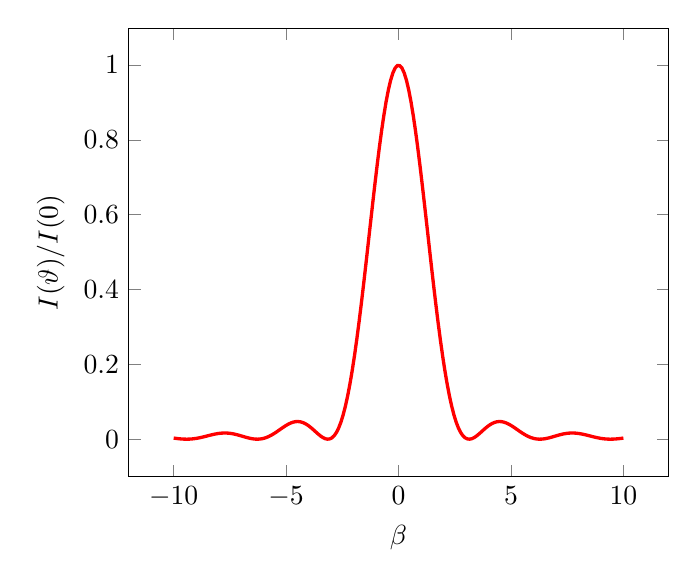
\begin{tikzpicture}
            \begin{axis}[xlabel=\(\beta\), ylabel={\(I(\vartheta)/I(0)\)}]
                \addplot[domain=-10:10, very thick, red, samples=200] {(sin(deg(x))/x)^2};
            \end{axis}
        \end{tikzpicture}
        \caption{The ratio of intensities, \(I(\vartheta)/I(0)\), as a function of \(\beta = (\pi a/\lambda)\sin\vartheta\)}
        \label{fig:sinc squared}
    \end{figure}

    \subsubsection{Slit and a Lens}
    We are considering only the far field limit as this allows us to approximate rays leaving the slit and arriving at the screen at the same point as parallel.
    Another way to make the same assumption is to place a lens of focal length \(f\) just after the slit.
    This causes parallel rays to converge at a point on the back focal plane, \(P_{f_b}\), which is a distance \(f\) from the lens.
    So a plane wave diffracted in the direction \(\vartheta\) will be focused at the point \(s = f\tan\vartheta \approx f\vartheta\).
    The intensity on the back focal plane will be
    \[I(s) = I_0\sinc^2\left( \frac{\pi as}{\lambda f} \right).\]
    This has zeros at
    \[s = n\frac{\lambda f}{a}, \qquad\text{for}\qquad n = \pm 1,\pm 2, \pm 3, \dotsc.\]
    The central maxima has width \(w = 2\lambda f/a\).
    Here we see again the reciprocal relationship between peak width and slit width.
    
    \subsection{Fourier Approach}
    Let \(f\colon\reals\to\complex\) have a Fourier transform.
    Then the Fourier transform is given by
    \[F(q) = \FT\{f(x)\} = \int_{-\infty}^{\infty} f(x) e^{iqx} \dd{x}.\]
    If \(f\colon\reals\to\reals\) then
    \[F(q) = \int_{-\infty}^{\infty} f(x)\cos(qx) \dd{x} + i\int_{-\infty}^{\infty} f(x)\sin(qx) \dd{x}.\]
    We can define a function, \(p\), which represents the slit:
    \[
        p(y) = 
        \begin{cases}
            1, & \abs{y} < a/2,\\
            0, & \abs{y} \ge a/2.
        \end{cases}
    \]
    We can rewrite equation~\ref{eqn:single slit amplitude} as
    \[\Re[E(\vartheta)] = \frac{\mathcal{A}}{R} \int_{-\infty}^{\infty} p(y)\cos\left( \frac{2\pi}{\lambda}y\sin\vartheta \right) \dd{y} = \frac{\mathcal{A}}{R}\Re[P(q)]\]
    where we take \(E\) to be the complex amplitude of the field and \(P(q) = \FT\{p(t)\}\) and \(q = (2\pi/\lambda)\sin\vartheta\).
    
    Similarly for the case of the slit and lens set up we have
    \[\Re[E(s)] = \frac{\mathcal{A}}{f} \int_{-\infty}^{\infty} p(y)\cos\left( \frac{2\pi}{\lambda}y\frac{s}{f} \right) \dd{y} = \frac{\mathcal{A}}{f}\Re[P(q)],\]
    where this time \(q = 2\pi s/(\lambda f)\).
    The intensity is then \(I(s) = I_0\abs{P(q)}^2\).
    So we see that the intensity in the back focal plane is proportional to the modulus squared of the Fourier transform of the function representing the slit.
    It can be shown that
    \[\FT\{p(x)\} = P(q) = a\sinc\left( \frac{aq}{2} \right).\]
    
    We can extend this to a two-dimensional slit which is rectangular with side lengths \(a\) and \(b\).
    This can be defined by the function
    \[
        p(x, y) =
        \begin{cases}
            1, & \abs{x} < a/2, \text{ and } \abs{y} < b/2,\\
            0, & \text{else.}
        \end{cases}
    \]
    The two-dimensional Fourier transform is then
    \[\FT\{p(x, y)\} = P(x, y) = ab\sinc\left( \frac{aq}{2} \right)\sinc\left( \frac{bp}{2} \right).\]
    Notice that we can write \(P\) and \(p\) as products of one-dimensional functions.
    This means that the intensity can be derived in the same way as above and we find that
    \[I(s, t) = I_0\sinc^2\left( \frac{\pi a s}{\lambda f} \right)\sinc^2\left( \frac{\pi b t}{\lambda f} \right).\]
    See figure~\ref{fig:rectangular slit}.
    \begin{figure}[ht]
        \centering
        \begin{subfigure}{0.9\textwidth}
            \centering
            \tikzsetnextfilename{rectangular-slit-intensity}
            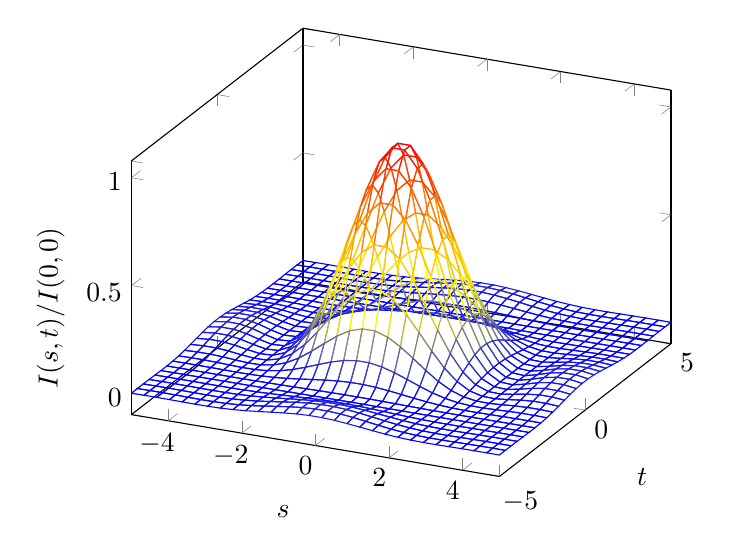
\begin{tikzpicture}
                \begin{axis}[
                    xlabel=\(s\),
                    ylabel=\(t\),
                    zlabel={\(I(s, t)/I(0, 0)\)},
                    xmin=-5,
                    xmax=5,
                    ymin=-5,
                    ymax=5,
                    samples=30
                    ]
                    \addplot3[
                    mesh,
                    colormap/hot
                    ] {(sin(deg(x))/x)^2 * (sin(deg(y))/y)^2};
                \end{axis}
            \end{tikzpicture}
            \caption{Intensity}
        \end{subfigure}
        \begin{subfigure}{0.9\textwidth}
            \centering
            \tikzsetnextfilename{rectangular-slit-log-intensity}
            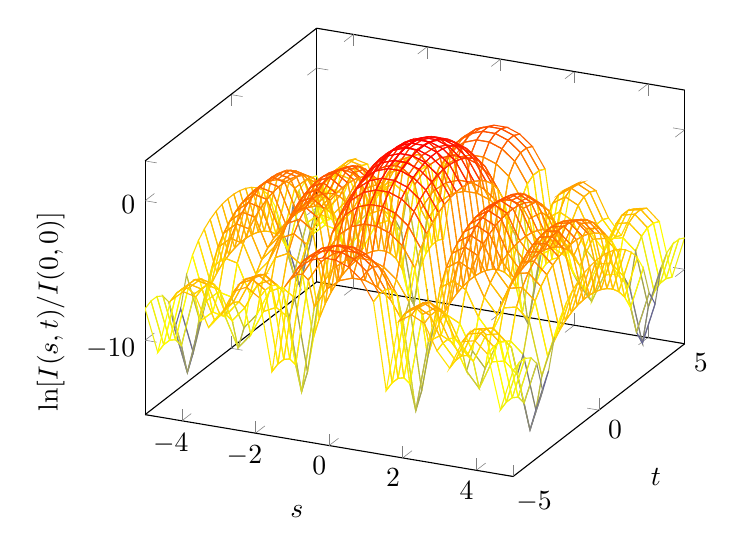
\begin{tikzpicture}
                \begin{axis}[
                    xlabel=\(s\),
                    ylabel=\(t\),
                    zlabel={\(\ln[I(s, t)/I(0, 0)]\)},
                    xmin=-5,
                    xmax=5,
                    ymin=-5,
                    ymax=5,
                    samples=30
                    ]
                    \addplot3[
                    mesh,
                    colormap/hot
                    ] {ln((sin(2*deg(x))/x)^2 * (sin(deg(y))/y)^2)};
                \end{axis}
            \end{tikzpicture}
            \caption{Log intensity.}
        \end{subfigure}
        \caption{The intensity, \(I(s, t)\), and log intensity, \(\ln[I(s, t)]\) of a slit of width \(2\) and height \(1\).}
        \label{fig:rectangular slit}
    \end{figure}

    \section{Two Slit Diffraction}
    We have now seen that the Fourier approach is a powerful one.
    We will apply it in this section to the famous two slit experiment.
    Let \(p\) be a single slit transition function for a slit of width \(a\) centred at \(x = 0\):
    \[
        p(x) = 
        \begin{cases}
            1, & \abs{x} < a/2,\\
            0, & \text{else.}
        \end{cases}
    \]
    We can then model two slits using delta distributions and a convolution:
    \[f(x) = p(x) \convolution \left[ \delta\left( x - \frac{d}{2} \right) + \delta\left( x + \frac{d}{2} \right) \right].\]
    Graphically this corresponds to
    \[
        \tikzsetnextfilename{double-slit-transmission-function}
        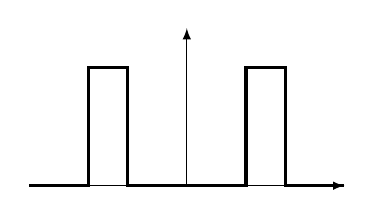
\begin{tikzpicture}[baseline=0, yshift=\axisht - 1cm]
            \draw[->, >=latex] (-2, 0) -- (2, 0);
            \draw[->, >=latex] (0, 0) -- (0, 2);
            \draw[very thick] (-2, 0) -- (-1.25, 0) -- (-1.25, 1.5) -- (-0.75, 1.5) -- (-0.75, 0) -- (0.75, 0) -- (0.75, 1.5) -- (1.25, 1.5) -- (1.25, 0) -- (2, 0);
        \end{tikzpicture}
        =
        \tikzsetnextfilename{single-slit-transmission-function}
        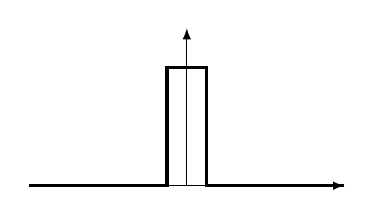
\begin{tikzpicture}[baseline=0, yshift=\axisht - 1cm]
            \draw[->, >=latex] (-2, 0) -- (2, 0);
            \draw[->, >=latex] (0, 0) -- (0, 2);
            \draw[very thick] (-2, 0) -- (-0.25, 0) -- (-0.25, 1.5) -- (0.25, 1.5) -- (0.25, 0) -- (2, 0);
        \end{tikzpicture}
        \convolution
        \tikzsetnextfilename{double-dirac-delta-distribution}
        \begin{tikzpicture}[baseline=0, yshift=\axisht - 1cm]
            \draw[->, >=latex] (-2, 0) -- (2, 0);
            \draw[->, >=latex] (0, 0) -- (0, 2);
            \draw[very thick] (-2, 0) -- (-1, 0) -- (-1, 2) -- (-1, 0) -- (1, 0) -- (1, 2) -- (1, 0) -- (2, 0);
        \end{tikzpicture}
    \]
    Using the convolution theorem we can write the Fourier transform of \(f\) as the product of the Fourier transforms of \(p\) and the delta distributions:
    \[F(q) = \sinc\left( \frac{aq}{2} \right)\cos\left( \frac{dq}{2} \right).\]
    The intensity is then
    \[I(\vartheta) = I_0\abs{F(q)}^2 = I_0\sinc^2\left( \frac{\pi a}{\lambda}\sin\vartheta \right)\cos^2\left( \frac{\pi d}{\lambda}\sin\vartheta \right).\]
    If we add in a lens of focal length \(f\) then
    \[I(s) = I_0\sinc^2\left( \frac{\pi a}{\lambda f}s \right)\cos^2\left( \frac{\pi d}{\lambda f}s \right).\]
    What we end up with is \(\cos^2\) fringes modulated by \(\sinc^2\), as can be seen in figure~\ref{fig:double slit intensity}.
    
    \begin{figure}[ht]
        \centering
        \tikzsetnextfilename{double-slit-intensity}
        \begin{tikzpicture}
            \begin{axis}[
                    xlabel=\(s\),
                    ylabel={\(I(s)/I(0)\)},
                    samples=300
                ]
                \addplot[
                    domain=-10:10,
                    very thick,
                    red
                ] {(sin(deg(x)) / x)^2 * cos(5*deg(x))^2};
                \addplot[gray, dashed, domain=-10:10]{((sin(deg(x))/x)^2};
                \addlegendentry{\(I(s)/I(0)\)}
                \addlegendentry{\(\sinc^2\)}
            \end{axis}
        \end{tikzpicture}
        \caption{The intensity from a double slit is \(\cos^2\) fringes modulated by \(\sinc^2\).}
        \label{fig:double slit intensity}
    \end{figure}
    
    This derivation was much quicker than the geometric argument that one has to make if they lack Fourier analysis.
    We can see that the extrema occur whenever the argument of \(\cos\) is \(n\pi\) or \((n + 1/2)\pi\) for \(n\in\integers\), which corresponds to 
    \[d\sin\vartheta = n\lambda, \qquad\text{or}\qquad d\sin\vartheta = (n + 1/2)\lambda\]
    which are the conditions for constructive and destructive interference respectively.
    
    \subsection{Diffraction Gratings}\label{sec:diffraction gratings}
    A diffraction grating is a large number of equally spaced thin slits.
    The phase difference between light from adjacent slits is
    \[\delta = \frac{2\pi}{\lambda}d\sin\vartheta\]
    where \(d\) is the space between adjacent slits.
    We know that wavelets will add constructively when \(\delta = 2\pi n\) for \(n\in\integers\).
    Therefore we expect peaks when
    \[d\sin\vartheta = n\lambda.\]
    If we include a lens of focal length \(f\) then we get peaks at
    \[s = n\frac{\lambda f}{d}.\]
    This doesn't tell us anything about the shapes of the peaks, just their locations, to get more information we again turn to Fourier analysis.
    
    If we approximate the number of slits as infinite and take the slits to have no width then we can then model the transmission function as a Dirac comb:
    \[c(x) = \sum_{m\in\integers} \delta(x - md).\]
    The Fourier transform of this is simple to compute and is
    \[C(q) = \frac{1}{d}\sum_{m\in\integers} \delta(q - 2\pi m/d).\]
    Notice that the spacing of the original comb, \(d\), is reciprocal to the spacing of the Fourier transformed comb, \(2\pi/d\).
    The intensity is then \(I(\vartheta) \propto \abs{C(q)}^2\).
    This is zero except when \(q = 2\pi m/d\) for \(m\in\integers\).
    Since \(q = (2\pi/\lambda)\sin\vartheta\) this corresponds to \(m\lambda = d\sin\vartheta\).
    This is the same condition we found before.
    
    This result is unrealistic as in reality there aren't an infinite number of slits and the slits have finite width.
    We can modify for the finite width by convolving the Dirac comb with a single slit transmission function, \(p\), and we can modify for the finite number of slits by multiplying by a top hat function, \(w\), of width \(D = Nd\) where \(N\) is the total number of slits.
    Thus the transmission function is
    \[f(x)= [c(x)\convolution p(x)]w(x).\]
    Graphically this is
    \[
        \tikzsetnextfilename{diffraction-grating-transmission-function}
        \begin{tikzpicture}[baseline=0, yshift=\axisht - 1cm]
            \draw[->, >=latex] (-1.5, 0) -- (1.5, 0);
            \draw[->, >=latex] (0, 0) -- (0, 2);
            \foreach \x in {-1, -0.75, ..., 1} {
                \draw (\x-0.1, 0) -- (\x-0.1, 0) -- (\x-0.1, 1.5) -- (\x+0.1, 1.5) -- (\x+0.1, 0);
            }
        \end{tikzpicture}
        =
        \tikzsetnextfilename{dirac-comb}
        \begin{tikzpicture}[baseline=0, yshift=\axisht - 1cm]
            \draw[decorate, decoration={brace, amplitude=5pt}] (-1.75, 0) -- (-1.75, 2);
            \draw[->, >=latex] (-1.5, 0) -- (1.5, 0);
            \draw[->, >=latex] (0, 0) -- (0, 2);
            \draw[very thick] (-1.5, 0) -- (1.5, 0);
            \foreach \x in {-1.25, -1, ..., 1.25} {
                \draw[very thick] (\x, 0) -- (\x, 2);
            }
        \end{tikzpicture}
        \convolution
        \tikzsetnextfilename{single-slit-transmission-function-again}
        \begin{tikzpicture}[baseline=0, yshift=\axisht - 1cm]
            \draw[->, >=latex] (-1.5, 0) -- (1.5, 0);
            \draw[->, >=latex] (0, 0) -- (0, 2);
            \draw[very thick] (-1.5, 0) -- (-0.1, 0) -- (-0.1, 1.5) -- (0.1, 1.5) -- (0.1, 0) -- (1.5, 0);
            \draw[decorate, decoration={brace, amplitude=5pt}] (1.75, 2) -- (1.75, 0);
        \end{tikzpicture}
        \tikzsetnextfilename{top-hat}
        \begin{tikzpicture}[baseline=0, yshift=\axisht - 1cm]
            \draw[->, >=latex] (-1.5, 0) -- (1.5, 0);
            \draw[->, >=latex] (0, 0) -- (0, 2);
            \draw[very thick] (-1.5, 0) -- (-1.2, 0) -- (-1.2, 1.5) -- (1.2, 1.5) -- (1.2, 0) -- (1.5, 0);
        \end{tikzpicture}
    \]
    By the convolution theorem the Fourier transform of the transmission function is
    \[F(x) = [W(q)\convolution C(q)]P(q).\]
    These functions are given by
    \begin{align*}
        C(q) &= \sum_{m\in\integers} \delta(q - 2\pi m/d),\\
        P(q) &= \sinc(aq/2),\\
        W(q) &= \sinc(Ndq/2).
    \end{align*}
    The intensity is
    \[I(\vartheta) = I(0)\abs{F(q)}^2 = I(0)\abs{F\left( \frac{2\pi}{\lambda}\sin\vartheta \right)}^2.\]
    
    \subsubsection{Spectroscopy}
    The intensity of light from a diffraction grating depends on the wave length, and therefore colour, of the light.
    So if a white light source is used we will see the colours separate out and each colour will have a maxima at a slightly different point.
    This makes diffraction gratings useful in spectroscopy.
    At this point we note that most diffraction gratings used for spectroscopy aren't actually made of lots of slits in an opaque material but rather a transparent medium with lots of thin parallel scratches.
    It is also common to instead use a reflection grating, which is basically the same but with reflective coating, such as aluminium.
    This is useful because glass absorbs strongly in the UV part of the spectrum and so glass transmission gratings don't work for UV light.
    
    A large amount of light from a diffraction grating ends up in the zeroth order, \(\vartheta = 0\), maxima.
    This is a problem because the intensity of this maxima \emph{doesn't} depend on \(\lambda\) making this fringe useless for spectroscopy.
    This is a problem if the light source we are using isn't very intense as the first order fringes, which can be used for spectroscopy, may be hard to see.
    One solution to this is to use a reflection grating with a surface that looks like this:
    \[\tikzsetnextfilename{blazed-grating}
        \tikz{
            \foreach \x in {1, 2, ..., 5} {
                \draw (\x, 0) -- (\x+1, 0.2) -- (\x+1, 0);
            }
        }
    \]
    This is called a blazed grating.
    Light that enters normal to the macroscopic surface is reflected mostly at an angle \(2\gamma\) where \(\gamma\), called the blazing angle, is the angle of the microscopic surface to the macroscopic surface.
    The zeroth order maxima from the diffraction however remains in the same place but is now much weaker.
    Instead by carefully selecting the blazing angle we can focus the majority of light onto where we expect the first order maxima to be and this light will be separated by wavelength.
    
    \section{More Diffraction}
    \subsection{Circular Aperture}
    It is very common for an optical system to have cylindrical symmetry about the beam axis, for example telescopes and microscopes.
    Therefore it is worth considering a circular aperture such as one might use for an eyepiece.
    The transmission function for a circular aperture of diameter \(a\) is
    \[
        p(x, y) =
        \begin{cases}
            1, & x^2 + y^2 \le a^2/4,\\
            0, & \text{else.}
        \end{cases}
    \]
    The Fourier transform of this is
    \[P(\rho) \propto \frac{J_1(\rho)}{\rho}\]
    where \(\rho = (\pi a/\lambda)\sin\vartheta\) and \(J_1\) is the first order Bessel function of the first kind, the exact details of which aren't important.
    The intensity at angle \(\vartheta\) is then
    \[I(\vartheta) = 4I(0) \abs{\frac{J_1([\pi a/\lambda]\sin\vartheta)}{(\pi a/\lambda)\sin\vartheta}}^2.\]
    If we include a lens of focal length \(f\) then the intensity at position \((s, t)\) on the back focal plane is
    \[I(s, t) = 4I(0, 0) = \abs{\frac{J_1(\pi ar/(\lambda f))}{\pi ar/(\lambda f)}}^2, \qquad\text{where}\qquad r^2 = s^2 + f^2.\]
    This result is very similar to the result of a single slit and has a similar profile at \(y = 0\) as shown in figure~\ref{fig:bessel funcs}.
    The first minimum occurs at \(\rho = 1.22\pi\), which corresponds to \(\sin\vartheta = 1.22\lambda/a\) (as opposed to \(\sin\vartheta = \lambda/a\) which we saw for a single slit).
    
    \begin{figure}[ht]
        \centering
        \begin{subfigure}{0.9\textwidth}
            \centering
            \tikzsetnextfilename{bessel-func}
            % This file was created by tikzplotlib v0.9.8.
\begin{tikzpicture}

\begin{axis}[
tick align=outside,
tick pos=left,
x grid style={white!69.0196078431373!black},
xlabel={\(\displaystyle \rho\)},
xmin=-11, xmax=11,
xtick style={color=black},
y grid style={white!69.0196078431373!black},
ylabel={\(\displaystyle P(\rho)\)},
ymin=-0.0943830110077863, ymax=0.528138630560538,
ytick style={color=black}
]
\addplot [very thick, red]
table {%
-10 0.00434727461688615
-9.89949748743719 0.00691894429722283
-9.79899497487437 0.00949924167703978
-9.69849246231156 0.0120628063659262
-9.59798994974874 0.0145836630228336
-9.49748743718593 0.0170354430428484
-9.39698492462312 0.0193916156872241
-9.2964824120603 0.021625726891485
-9.19597989949749 0.0237116438868739
-9.09547738693467 0.0256238036849729
-8.99497487437186 0.027337463404914
-8.89447236180905 0.0288289503680182
-8.79396984924623 0.0300759098466582
-8.69346733668342 0.0310575483331712
-8.5929648241206 0.0317548701911897
-8.49246231155779 0.0321509055660751
-8.39195979899498 0.0322309274633623
-8.29145728643216 0.0319826559542405
-8.19095477386935 0.0313964475349253
-8.09045226130653 0.0304654677520127
-7.98994974874372 0.0291858453080579
-7.8894472361809 0.0275568059800957
-7.78894472361809 0.0255807848178281
-7.68844221105528 0.0232635152368735
-7.58793969849246 0.020614093784748
-7.48743718592965 0.0176450195319828
-7.38693467336683 0.0143722072267061
-7.28643216080402 0.010814973546732
-7.18592964824121 0.00699599598724522
-7.08542713567839 0.00294124413297328
-6.98492462311558 -0.00132011672034047
-6.88442211055276 -0.0057558494109933
-6.78391959798995 -0.0103307958177117
-6.68341708542714 -0.0150070542012278
-6.58291457286432 -0.0197441821358482
-6.48241206030151 -0.0244994239704469
-6.38190954773869 -0.0292279615484125
-6.28140703517588 -0.0338831867134029
-6.18090452261307 -0.0384169939340305
-6.08040201005025 -0.0427800911974767
-5.97989949748744 -0.0469223271511087
-5.87939698492462 -0.0507930323139475
-5.77889447236181 -0.054341372037735
-5.67839195979899 -0.0575167087716571
-5.57788944723618 -0.0602689710766938
-5.47738693467337 -0.0625490267461231
-5.37688442211055 -0.0643090573188185
-5.27638190954774 -0.0655029312224057
-5.17587939698492 -0.0660865727546806
-5.07537688442211 -0.0660183241043791
-4.9748743718593 -0.0652592976266965
-4.87437185929648 -0.0637737156249773
-4.77386934673367 -0.0615292349476604
-4.67336683417085 -0.0584972537886211
-4.57286432160804 -0.0546531981790696
-4.47236180904523 -0.0499767857795613
-4.37185929648241 -0.0444522647206739
-4.2713567839196 -0.0380686253995941
-4.17085427135678 -0.0308197833161446
-4.07035175879397 -0.0227047312244492
-3.96984924623116 -0.0137276590840981
-3.86934673366834 -0.0038980405158586
-3.76884422110553 0.00676931529995345
-3.66834170854271 0.0182542471010835
-3.5678391959799 0.0305312609639628
-3.46733668341709 0.0435695859763079
-3.36683417085427 0.0573332662080615
-3.26633165829146 0.0717812887619347
-3.16582914572864 0.0868677474192174
-3.06532663316583 0.102542041132504
-2.96482412060301 0.118749106356568
-2.8643216080402 0.135429681953857
-2.76381909547739 0.15252060516396
-2.66331658291457 0.169955136888865
-2.56281407035176 0.187663314319774
-2.46231155778894 0.20557232871844
-2.36180904522613 0.223606925968226
-2.26130653266332 0.241689827328801
-2.1608040201005 0.259742167665257
-2.06030150753769 0.277683948278612
-1.95979899497487 0.295434501341436
-1.85929648241206 0.312912962840766
-1.75879396984925 0.330038750851305
-1.65829145728643 0.34673204590599
-1.55778894472362 0.362914270198756
-1.4572864321608 0.378508562346094
-1.35678391959799 0.393440244449982
-1.25628140703517 0.407637278244869
-1.15577889447236 0.42103070717541
-1.05527638190955 0.433555081339157
-0.954773869346733 0.445148862338856
-0.854271356783919 0.455754805221492
-0.753768844221105 0.465320314834966
-0.653266331658291 0.473797774107009
-0.552763819095476 0.481144841943462
-0.452261306532662 0.487324718652916
-0.351758793969848 0.492306377030342
-0.251256281407034 0.496064757472071
-0.15075376884422 0.498580925746513
-0.0502512562814061 0.499842192307433
0.0502512562814079 0.499842192307433
0.150753768844222 0.498580925746513
0.251256281407036 0.496064757472071
0.35175879396985 0.492306377030342
0.452261306532664 0.487324718652916
0.552763819095478 0.481144841943462
0.653266331658292 0.473797774107009
0.753768844221106 0.465320314834966
0.85427135678392 0.455754805221492
0.954773869346734 0.445148862338856
1.05527638190955 0.433555081339157
1.15577889447236 0.42103070717541
1.25628140703518 0.407637278244869
1.35678391959799 0.393440244449981
1.4572864321608 0.378508562346094
1.55778894472362 0.362914270198756
1.65829145728643 0.34673204590599
1.75879396984925 0.330038750851305
1.85929648241206 0.312912962840766
1.95979899497488 0.295434501341436
2.06030150753769 0.277683948278612
2.1608040201005 0.259742167665257
2.26130653266332 0.241689827328801
2.36180904522613 0.223606925968226
2.46231155778895 0.20557232871844
2.56281407035176 0.187663314319773
2.66331658291457 0.169955136888865
2.76381909547739 0.15252060516396
2.8643216080402 0.135429681953857
2.96482412060302 0.118749106356568
3.06532663316583 0.102542041132504
3.16582914572864 0.0868677474192173
3.26633165829146 0.0717812887619346
3.36683417085427 0.0573332662080615
3.46733668341709 0.0435695859763077
3.5678391959799 0.0305312609639627
3.66834170854271 0.0182542471010833
3.76884422110553 0.00676931529995336
3.86934673366834 -0.00389804051585869
3.96984924623116 -0.0137276590840982
4.07035175879397 -0.0227047312244493
4.17085427135678 -0.0308197833161447
4.2713567839196 -0.0380686253995941
4.37185929648241 -0.044452264720674
4.47236180904523 -0.0499767857795614
4.57286432160804 -0.0546531981790697
4.67336683417085 -0.0584972537886211
4.77386934673367 -0.0615292349476604
4.87437185929648 -0.0637737156249773
4.9748743718593 -0.0652592976266965
5.07537688442211 -0.0660183241043791
5.17587939698493 -0.0660865727546806
5.27638190954774 -0.0655029312224057
5.37688442211055 -0.0643090573188185
5.47738693467337 -0.0625490267461231
5.57788944723618 -0.0602689710766938
5.678391959799 -0.057516708771657
5.77889447236181 -0.0543413720377349
5.87939698492462 -0.0507930323139475
5.97989949748744 -0.0469223271511087
6.08040201005025 -0.0427800911974766
6.18090452261307 -0.0384169939340305
6.28140703517588 -0.0338831867134029
6.38190954773869 -0.0292279615484125
6.48241206030151 -0.0244994239704468
6.58291457286432 -0.0197441821358482
6.68341708542714 -0.0150070542012277
6.78391959798995 -0.0103307958177117
6.88442211055277 -0.00575584941099323
6.98492462311558 -0.00132011672034047
7.08542713567839 0.00294124413297328
7.18592964824121 0.00699599598724522
7.28643216080402 0.010814973546732
7.38693467336683 0.0143722072267061
7.48743718592965 0.0176450195319827
7.58793969849246 0.020614093784748
7.68844221105528 0.0232635152368736
7.78894472361809 0.0255807848178281
7.88944723618091 0.0275568059800958
7.98994974874372 0.0291858453080579
8.09045226130653 0.0304654677520127
8.19095477386935 0.0313964475349253
8.29145728643216 0.0319826559542405
8.39195979899498 0.0322309274633623
8.49246231155779 0.032150905566075
8.5929648241206 0.0317548701911897
8.69346733668342 0.0310575483331712
8.79396984924623 0.0300759098466582
8.89447236180905 0.0288289503680182
8.99497487437186 0.027337463404914
9.09547738693468 0.0256238036849729
9.19597989949749 0.0237116438868739
9.2964824120603 0.021625726891485
9.39698492462312 0.0193916156872241
9.49748743718593 0.0170354430428483
9.59798994974874 0.0145836630228336
9.69849246231156 0.0120628063659262
9.79899497487437 0.00949924167703978
9.89949748743719 0.00691894429722276
10 0.00434727461688615
};
\end{axis}

\end{tikzpicture}

            \caption{\(P(\rho) \propto J_1(\rho)/\rho\).}
        \end{subfigure}
        \begin{subfigure}{0.9\textwidth}
            \centering
            \tikzsetnextfilename{bessel-func-squared}
            % This file was created by tikzplotlib v0.9.8.
\begin{tikzpicture}

\begin{axis}[
tick align=outside,
tick pos=left,
x grid style={white!69.0196078431373!black},
xlabel={\(\displaystyle \rho\)},
xmin=-11, xmax=11,
xtick style={color=black},
y grid style={white!69.0196078431373!black},
ylabel={\(\displaystyle \abs{P(\rho)}^2\)},
ymin=-0.0124902810169719, ymax=0.262334240935828,
ytick style={color=black}
]
\addplot [very thick, red]
table {%
-10 1.88987965946226e-05
-9.89949748743719 4.78717901880723e-05
-9.79899497487437 9.02355924388096e-05
-9.69849246231156 0.000145511297421831
-9.59798994974874 0.000212683227163565
-9.49748743718593 0.000290206319666131
-9.39698492462312 0.000376034758960994
-9.2964824120603 0.000467672063585098
-9.19597989949749 0.000562242055817925
-9.09547738693467 0.000656579315286033
-8.99497487437186 0.000747336905415011
-8.89447236180905 0.000831108379321656
-8.79396984924623 0.000904560353104314
-8.69346733668342 0.000964571308467265
-8.5929648241206 0.00100837178085931
-8.49246231155779 0.00103368072871868
-8.39195979899498 0.00103883268514853
-8.29145728643216 0.00102289028188732
-8.19095477386935 0.00098573691781332
-8.09045226130653 0.000928144725348923
-7.98994974874372 0.000851813566345888
-7.8894472361809 0.000759377555824641
-7.78894472361809 0.000654376551896023
-7.68844221105528 0.000541191141176245
-7.58793969849246 0.000424940862566385
-7.48743718592965 0.000311346714284053
-7.38693467336683 0.000206560340567382
-7.28643216080402 0.000116963652816512
-7.18592964824121 4.89439598535512e-05
-7.08542713567839 8.65091704974974e-06
-6.98492462311558 1.74270815532249e-06
-6.88442211055276 3.31298024420319e-05
-6.78391959798995 0.00010672534222725
-6.68341708542714 0.00022521167579859
-6.58291457286432 0.000389832728213547
-6.48241206030151 0.000600221774883706
-6.38190954773869 0.000854273736275481
-6.28140703517588 0.00114807034185532
-6.18090452261307 0.00147586542292734
-6.08040201005025 0.00183013620286443
-5.97989949748744 0.00220170478527567
-5.87939698492462 0.00257993213164572
-5.77889447236181 0.00295298471494353
-5.67839195979899 0.00330817178792361
-5.57788944723618 0.00363234887464336
-5.47738693467337 0.00391238074688723
-5.37688442211055 0.00413565485323509
-5.27638190954774 0.00429063399872722
-5.17587939698492 0.0043674350984597
-5.07537688442211 0.00435841911755084
-4.9748743718593 0.00425877592672976
-4.87437185929648 0.00406708680461547
-4.77386934673367 0.00378584675324439
-4.67336683417085 0.00342192870081034
-4.57286432160804 0.00298697207120066
-4.47236180904523 0.00249767911685616
-4.37185929648241 0.00197600383879687
-4.2713567839196 0.00144922023981462
-4.17085427135678 0.000949859043654106
-4.07035175879397 0.00051550481997448
-3.96984924623116 0.000188448623929221
-3.86934673366834 1.51947198632752e-05
-3.76884422110553 4.58236296301839e-05
-3.66834170854271 0.000333217537227417
-3.5678391959799 0.000932157896049601
-3.46733668341709 0.00189830882214689
-3.36683417085427 0.00328710341408445
-3.26633165829146 0.00515255341632425
-3.16582914572864 0.00754600554168895
-3.06532663316583 0.0105148701996202
-2.96482412060301 0.0141013502604835
-2.8643216080402 0.0183411987541228
-2.76381909547739 0.0232625349995805
-2.66331658291457 0.0288847485549129
-2.56281407035176 0.0352175195414821
-2.46231155778894 0.0422599823347224
-2.36180904522613 0.0500000573409598
-2.26130653266332 0.0584139726342257
-2.1608040201005 0.0674659936634467
-2.06030150753769 0.0771083751315987
-1.95979899497487 0.087281544582863
-1.85929648241206 0.0979145223137868
-1.75879396984925 0.10892557706349
-1.65829145728643 0.120223111658154
-1.55778894472362 0.131706767513896
-1.4572864321608 0.143268731769307
-1.35678391959799 0.154795225952861
-1.25628140703517 0.166168150614885
-1.15577889447236 0.177266856384626
-1.05527638190955 0.187970008555003
-0.954773869346733 0.198157509641578
-0.854271356783919 0.20771244248248
-0.753768844221105 0.216522995398112
-0.653266331658291 0.224484330748757
-0.552763819095476 0.231500358928799
-0.452261306532662 0.237485381410144
-0.351758793969848 0.242365568864742
-0.251256281407034 0.246080243605825
-0.15075376884422 0.24858293951825
-0.0502512562814061 0.249842217210701
0.0502512562814079 0.249842217210701
0.150753768844222 0.24858293951825
0.251256281407036 0.246080243605825
0.35175879396985 0.242365568864742
0.452261306532664 0.237485381410144
0.552763819095478 0.231500358928799
0.653266331658292 0.224484330748757
0.753768844221106 0.216522995398112
0.85427135678392 0.20771244248248
0.954773869346734 0.198157509641578
1.05527638190955 0.187970008555003
1.15577889447236 0.177266856384626
1.25628140703518 0.166168150614885
1.35678391959799 0.154795225952861
1.4572864321608 0.143268731769307
1.55778894472362 0.131706767513895
1.65829145728643 0.120223111658153
1.75879396984925 0.10892557706349
1.85929648241206 0.0979145223137865
1.95979899497488 0.0872815445828628
2.06030150753769 0.0771083751315986
2.1608040201005 0.0674659936634466
2.26130653266332 0.0584139726342256
2.36180904522613 0.0500000573409597
2.46231155778895 0.0422599823347223
2.56281407035176 0.0352175195414821
2.66331658291457 0.0288847485549129
2.76381909547739 0.0232625349995804
2.8643216080402 0.0183411987541228
2.96482412060302 0.0141013502604834
3.06532663316583 0.0105148701996201
3.16582914572864 0.00754600554168893
3.26633165829146 0.00515255341632423
3.36683417085427 0.00328710341408444
3.46733668341709 0.00189830882214687
3.5678391959799 0.000932157896049593
3.66834170854271 0.000333217537227409
3.76884422110553 4.58236296301827e-05
3.86934673366834 1.51947198632759e-05
3.96984924623116 0.000188448623929224
4.07035175879397 0.000515504819974484
4.17085427135678 0.00094985904365411
4.2713567839196 0.00144922023981462
4.37185929648241 0.00197600383879688
4.47236180904523 0.00249767911685617
4.57286432160804 0.00298697207120066
4.67336683417085 0.00342192870081035
4.77386934673367 0.0037858467532444
4.87437185929648 0.00406708680461547
4.9748743718593 0.00425877592672976
5.07537688442211 0.00435841911755084
5.17587939698493 0.00436743509845969
5.27638190954774 0.00429063399872721
5.37688442211055 0.00413565485323509
5.47738693467337 0.00391238074688722
5.57788944723618 0.00363234887464335
5.678391959799 0.00330817178792361
5.77889447236181 0.00295298471494352
5.87939698492462 0.00257993213164571
5.97989949748744 0.00220170478527567
6.08040201005025 0.00183013620286442
6.18090452261307 0.00147586542292734
6.28140703517588 0.00114807034185532
6.38190954773869 0.000854273736275481
6.48241206030151 0.000600221774883703
6.58291457286432 0.000389832728213547
6.68341708542714 0.000225211675798585
6.78391959798995 0.00010672534222725
6.88442211055277 3.31298024420311e-05
6.98492462311558 1.74270815532249e-06
7.08542713567839 8.65091704974973e-06
7.18592964824121 4.89439598535512e-05
7.28643216080402 0.000116963652816513
7.38693467336683 0.000206560340567382
7.48743718592965 0.000311346714284053
7.58793969849246 0.000424940862566385
7.68844221105528 0.000541191141176251
7.78894472361809 0.000654376551896023
7.88944723618091 0.000759377555824642
7.98994974874372 0.000851813566345888
8.09045226130653 0.000928144725348925
8.19095477386935 0.00098573691781332
8.29145728643216 0.00102289028188732
8.39195979899498 0.00103883268514853
8.49246231155779 0.00103368072871868
8.5929648241206 0.00100837178085931
8.69346733668342 0.000964571308467263
8.79396984924623 0.000904560353104314
8.89447236180905 0.000831108379321655
8.99497487437186 0.000747336905415011
9.09547738693468 0.000656579315286031
9.19597989949749 0.000562242055817925
9.2964824120603 0.000467672063585096
9.39698492462312 0.000376034758960994
9.49748743718593 0.000290206319666129
9.59798994974874 0.000212683227163565
9.69849246231156 0.00014551129742183
9.79899497487437 9.02355924388096e-05
9.89949748743719 4.78717901880714e-05
10 1.88987965946226e-05
};
\end{axis}

\end{tikzpicture}

            \caption{\(I(\rho) \propto \abs{P(\rho)}^2 \propto \abs{J_1(\rho)/\rho}^2\).}
        \end{subfigure}
        \caption{The Fourier transform, \(P\), of the transmission function \(p(x, y) = 1\) if \(x^2 + y^2 \le a^2/4\) and \(p(x, y) = \) otherwise, and the intensity of the light that results from this circular aperture.}
        \label{fig:bessel funcs}
    \end{figure}
    The function \(J_1(\rho)/\rho\) is actually two-dimensional with \(\rho\) just being the distance from the origin.
    The is plotted in figure~\ref{fig:bessel funcs 3d}.
    \begin{figure}[htbp!]
        \centering
        \begin{subfigure}{0.45\textwidth}
            \centering
            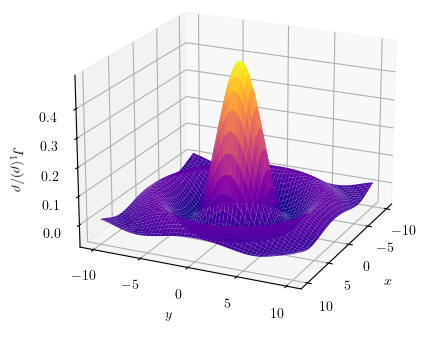
\includegraphics[scale=0.5]{bessel_func.png}
            \caption{\(J_1(\sqrt{x^2 + y^2})/\sqrt{x^2 + y^2}.\)}
        \end{subfigure}
        \begin{subfigure}{0.45\textwidth}
            \centering
            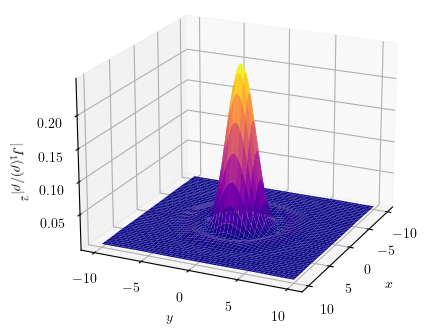
\includegraphics[scale=0.5]{bessel_func_squared.png}
            \caption{\(\abs{J_1(\sqrt{x^2 + y^2})/\sqrt{x^2 + y^2}}^2.\)}
        \end{subfigure}
        \caption{The functions \(J_1(\sqrt{x^2 + y^2})/\sqrt{x^2 + y^2}\) and \(\abs{J_1(\sqrt{x^2 + y^2})/\sqrt{x^2 + y^2}}^2\).}
        \label{fig:bessel funcs 3d}
    \end{figure}
    
    Suppose we view a distant point object through a lens of focal length \(f\) and diameter \(a\).
    The lens is circular so in the back focal plane of the lens we will get a diffraction pattern corresponding to a circular aperture.
    This has the first zero at radius
    \[r_0 = \frac{1.22 \lambda f}{a} = 1.22\lambda F_{\mathrm{No}}.\]
    Here we have introduced the \define{\(f\)-number}, \(F_\mathrm{no} = f/a\) which is the ratio of the focal length and aperture.
    This number is important in photography, where it is usually written as \(f/F_{\mathrm{No}}\), with \(f\) left as \(f\) but \(F_{\mathrm{No}}\) replaced with a number, for example \(f/2.8\), if we substitute for the focal length as well then we would get the aperture of the lens.
    If \(F_{\mathrm{No}}\) is large then a photograph will have a blurred background as the intensity of light from each point is very spread out.
    If \(F_{\mathrm{No}}\) is small then the photograph will have a sharp background as the intensity drops to zero very quickly.
    round the image of the point object there will be rings, known as \define{Airy rings}, and the whole pattern that appears from a single point object is called the \define{point spread function}.
    
    The point spread function limits the spatial resolution of the system.
    If two point objects have angular separation \(\Delta\vartheta\) then in the back focal plane of the lens we will have two point spread functions with their peaks separated by \(s = f\Delta \vartheta\) (assuming \(\Delta\vartheta\ll 1\)).
    There are three possibilities:
    \begin{itemize}
        \item[\(s \gg r_0\)] Two well separated point spread functions, it is easy to tell the two points apart.
        \item[\(s \ll r_0\)] The two point spread functions merge and it is not possible to tell the two points apart.
        \item[\(s\approx r_0\)] There will be some limit at which we say the points are resolved.
    \end{itemize}
    The \define{Rayleigh criterion} states that two points are first resolved when \(s = r_0\).
    Under this condition the peak of one point spread function appears at the zero of the other resulting in a twin peak with a \SI{20}{\percent} dip in the middle.
    This corresponds to the angular condition that
    \[\Delta\vartheta = 122\frac{\lambda}{a}.\]
    See figure~\ref{fig:two points}.
    \begin{figure}[htb]
        \centering
        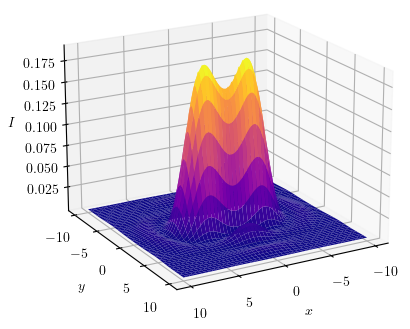
\includegraphics[scale=0.8]{two_points.png}
        \caption{The intensity on the back focal plane for two points at separation \(s = 5\).}
        \label{fig:two points}
    \end{figure}
    
    \section{Even More Diffraction}
    \subsection{Diffraction in 1D}
    When we first considered diffraction gratings in section~\ref{sec:diffraction gratings} we considered the slits to be narrow in one dimension and infinitely long in the orthogonal direction.
    The incident light was normal to both of these axes.
    If we truly restrict ourselves to one dimensional slits then we can consider non-normal incidence.
    If light is incident on the diffraction grating (either a transmission or reflection grating) at an angle \(\vartheta_i\) to the surface normal and leaves the grating at an angle \(\vartheta_m\) to the surface normal then the condition for constructive interference is
    \[m\lambda = d(\sin\vartheta_m - \sin\vartheta_i)\]
    for \(m\in\integers\).
    As \(\vartheta_i\) is increased from 0 to \(\pi/2\) then we lose diffraction peaks with \(m > 0\) and gain higher order peaks for negative \(m\).
    For grazing incidence at \(\vartheta_i = \pi/2\) the condition for constructive interference reduces to
    \[\sin\vartheta_m = \frac{m\lambda}{d} + 1.\]
    As well as this since the light simply passes straight past the diffraction grating we require that \(\vartheta_m = \pm \pi/2\).
    The case of \(\vartheta_m = \pi/2\) corresponds to \(m = 0\) so the zeroth order peak is directly ahead.
    The case of \(\vartheta_m = -\pi/2\) corresponds to \(-m\lambda = 2d\) which corresponds to the beam heading back the way it came.
    This returning beam can only exist if \(d\) is equal to an integer number of half-wavelengths, or if \(k = m\pi/d\).
    
    \subsection{X-ray Diffraction}
    Moving back to three dimensions consider an array of identical holes.
    We expect the diffraction pattern to be the superposition of the diffraction patterns from each hole.
    As with the initial diffraction grating we can describe the transmission function with a convolution of single hole transmission function and a two dimensional Dirac comb.
    We can then deal with the finite extent of the grating by multiplying by a two dimensional top hat function.
    Once we've done this we simply take the square of the Fourier transform for the intensity.
    The Fourier transform is easy to find if the scattering centres are evenly distributed, in particular they are located at \(\vv{R} = l\vv{a} + m\vv{b}\) for \(l, m\in\integers\), and basis vectors \(\vv{a}\) and \(\vv{b}\).
    
    We can also consider a three dimensional diffraction grating.
    The most common example being a crystalline solid.
    The repeat distance in this case is the interatomic spacing, which is on the order of \(\SI{e-10}{\metre}\), which is about four orders of magnitude smaller than the wavelength of visible light.
    This means that visible light will display only the first order diffraction, which isn't very useful.
    Instead we use X-rays.
    Again we can decompose the system into scattering units with some given transmission function that we then replicate through space by convolution with a three-dimensional Dirac comb and multiplication by some three-dimensional top hat function.
    Taking \(\{\vv{a}, \vv{b}, \vv{c}\}\) as basis vectors then we have a scattering unit at each \(\vv{R} = l\vv{a} + m\vv{b} + n\vv{c}\) for \(l, m, n\in\integers\).
    The set of all such \(\vv{R}\) gives all of the locations and we can distinguish any one such point with three numbers, \((l, m, n)\).
    Consider one particular, but arbitrary, scattering centre positioned at \(\vv{R}\).
    It can be shown that there will be constructive interference if and only if
    \[\vv{R}\cdot(\vv{k} - \vv{k'}) = 2\pi q\]
    for some \(q\in\integers\).
    Here \(\vv{k}\) and \(\vv{k'}\) are the wave vectors of the incident and scattered rays.
    All scattering sites which are an integer multiple of \(\vv{R}\) away from this original scattering centre will also contribute constructively to the interference.
    There are a few observations to be made:
    \begin{itemize}
        \item The wave vectors, \(\vv{K}\), satisfying \(\vv{R}\cdot\vv{K} = 2\pi q\) for some \(q\in\integers\) are special.
        The correspond to harmonic waves with the same periodicity as the lattice.
        These are the waves that appear in the Fourier series of the lattice.
        \item This allows us to state the constructive interference condition generally as \(\vv{k} - \vv{k'} = \vv{K}\).
        \item We can also use Fourier methods to find the intensity as well as just the extrema, this requires us to take a Fourier transform of the electron density surrounding each scattering centre as it is the electrons that are responsible for scattering the X-rays.
    \end{itemize}
\end{document}
